\documentclass[]{book}
\usepackage{lmodern}
\usepackage{amssymb,amsmath}
\usepackage{ifxetex,ifluatex}
\usepackage{fixltx2e} % provides \textsubscript
\ifnum 0\ifxetex 1\fi\ifluatex 1\fi=0 % if pdftex
  \usepackage[T1]{fontenc}
  \usepackage[utf8]{inputenc}
\else % if luatex or xelatex
  \ifxetex
    \usepackage{mathspec}
  \else
    \usepackage{fontspec}
  \fi
  \defaultfontfeatures{Ligatures=TeX,Scale=MatchLowercase}
\fi
% use upquote if available, for straight quotes in verbatim environments
\IfFileExists{upquote.sty}{\usepackage{upquote}}{}
% use microtype if available
\IfFileExists{microtype.sty}{%
\usepackage{microtype}
\UseMicrotypeSet[protrusion]{basicmath} % disable protrusion for tt fonts
}{}
\usepackage{hyperref}
\hypersetup{unicode=true,
            pdftitle={Notas de clase del curso de introducción a Data Science},
            pdfauthor={Diego Kozlowski y Natsumi Shokida},
            pdfborder={0 0 0},
            breaklinks=true}
\urlstyle{same}  % don't use monospace font for urls
\usepackage{natbib}
\bibliographystyle{apalike}
\usepackage{color}
\usepackage{fancyvrb}
\newcommand{\VerbBar}{|}
\newcommand{\VERB}{\Verb[commandchars=\\\{\}]}
\DefineVerbatimEnvironment{Highlighting}{Verbatim}{commandchars=\\\{\}}
% Add ',fontsize=\small' for more characters per line
\usepackage{framed}
\definecolor{shadecolor}{RGB}{248,248,248}
\newenvironment{Shaded}{\begin{snugshade}}{\end{snugshade}}
\newcommand{\AlertTok}[1]{\textcolor[rgb]{0.94,0.16,0.16}{#1}}
\newcommand{\AnnotationTok}[1]{\textcolor[rgb]{0.56,0.35,0.01}{\textbf{\textit{#1}}}}
\newcommand{\AttributeTok}[1]{\textcolor[rgb]{0.77,0.63,0.00}{#1}}
\newcommand{\BaseNTok}[1]{\textcolor[rgb]{0.00,0.00,0.81}{#1}}
\newcommand{\BuiltInTok}[1]{#1}
\newcommand{\CharTok}[1]{\textcolor[rgb]{0.31,0.60,0.02}{#1}}
\newcommand{\CommentTok}[1]{\textcolor[rgb]{0.56,0.35,0.01}{\textit{#1}}}
\newcommand{\CommentVarTok}[1]{\textcolor[rgb]{0.56,0.35,0.01}{\textbf{\textit{#1}}}}
\newcommand{\ConstantTok}[1]{\textcolor[rgb]{0.00,0.00,0.00}{#1}}
\newcommand{\ControlFlowTok}[1]{\textcolor[rgb]{0.13,0.29,0.53}{\textbf{#1}}}
\newcommand{\DataTypeTok}[1]{\textcolor[rgb]{0.13,0.29,0.53}{#1}}
\newcommand{\DecValTok}[1]{\textcolor[rgb]{0.00,0.00,0.81}{#1}}
\newcommand{\DocumentationTok}[1]{\textcolor[rgb]{0.56,0.35,0.01}{\textbf{\textit{#1}}}}
\newcommand{\ErrorTok}[1]{\textcolor[rgb]{0.64,0.00,0.00}{\textbf{#1}}}
\newcommand{\ExtensionTok}[1]{#1}
\newcommand{\FloatTok}[1]{\textcolor[rgb]{0.00,0.00,0.81}{#1}}
\newcommand{\FunctionTok}[1]{\textcolor[rgb]{0.00,0.00,0.00}{#1}}
\newcommand{\ImportTok}[1]{#1}
\newcommand{\InformationTok}[1]{\textcolor[rgb]{0.56,0.35,0.01}{\textbf{\textit{#1}}}}
\newcommand{\KeywordTok}[1]{\textcolor[rgb]{0.13,0.29,0.53}{\textbf{#1}}}
\newcommand{\NormalTok}[1]{#1}
\newcommand{\OperatorTok}[1]{\textcolor[rgb]{0.81,0.36,0.00}{\textbf{#1}}}
\newcommand{\OtherTok}[1]{\textcolor[rgb]{0.56,0.35,0.01}{#1}}
\newcommand{\PreprocessorTok}[1]{\textcolor[rgb]{0.56,0.35,0.01}{\textit{#1}}}
\newcommand{\RegionMarkerTok}[1]{#1}
\newcommand{\SpecialCharTok}[1]{\textcolor[rgb]{0.00,0.00,0.00}{#1}}
\newcommand{\SpecialStringTok}[1]{\textcolor[rgb]{0.31,0.60,0.02}{#1}}
\newcommand{\StringTok}[1]{\textcolor[rgb]{0.31,0.60,0.02}{#1}}
\newcommand{\VariableTok}[1]{\textcolor[rgb]{0.00,0.00,0.00}{#1}}
\newcommand{\VerbatimStringTok}[1]{\textcolor[rgb]{0.31,0.60,0.02}{#1}}
\newcommand{\WarningTok}[1]{\textcolor[rgb]{0.56,0.35,0.01}{\textbf{\textit{#1}}}}
\usepackage{longtable,booktabs}
\usepackage{graphicx,grffile}
\makeatletter
\def\maxwidth{\ifdim\Gin@nat@width>\linewidth\linewidth\else\Gin@nat@width\fi}
\def\maxheight{\ifdim\Gin@nat@height>\textheight\textheight\else\Gin@nat@height\fi}
\makeatother
% Scale images if necessary, so that they will not overflow the page
% margins by default, and it is still possible to overwrite the defaults
% using explicit options in \includegraphics[width, height, ...]{}
\setkeys{Gin}{width=\maxwidth,height=\maxheight,keepaspectratio}
\IfFileExists{parskip.sty}{%
\usepackage{parskip}
}{% else
\setlength{\parindent}{0pt}
\setlength{\parskip}{6pt plus 2pt minus 1pt}
}
\setlength{\emergencystretch}{3em}  % prevent overfull lines
\providecommand{\tightlist}{%
  \setlength{\itemsep}{0pt}\setlength{\parskip}{0pt}}
\setcounter{secnumdepth}{5}
% Redefines (sub)paragraphs to behave more like sections
\ifx\paragraph\undefined\else
\let\oldparagraph\paragraph
\renewcommand{\paragraph}[1]{\oldparagraph{#1}\mbox{}}
\fi
\ifx\subparagraph\undefined\else
\let\oldsubparagraph\subparagraph
\renewcommand{\subparagraph}[1]{\oldsubparagraph{#1}\mbox{}}
\fi

%%% Use protect on footnotes to avoid problems with footnotes in titles
\let\rmarkdownfootnote\footnote%
\def\footnote{\protect\rmarkdownfootnote}

%%% Change title format to be more compact
\usepackage{titling}

% Create subtitle command for use in maketitle
\providecommand{\subtitle}[1]{
  \posttitle{
    \begin{center}\large#1\end{center}
    }
}

\setlength{\droptitle}{-2em}

  \title{Notas de clase del curso de introducción a Data Science}
    \pretitle{\vspace{\droptitle}\centering\huge}
  \posttitle{\par}
    \author{Diego Kozlowski y Natsumi Shokida}
    \preauthor{\centering\large\emph}
  \postauthor{\par}
      \predate{\centering\large\emph}
  \postdate{\par}
    \date{2019-09-01}

\usepackage{booktabs}
\usepackage{amsthm}
\makeatletter
\def\thm@space@setup{%
  \thm@preskip=8pt plus 2pt minus 4pt
  \thm@postskip=\thm@preskip
}
\makeatother

\begin{document}
\maketitle

{
\setcounter{tocdepth}{1}
\tableofcontents
}
\hypertarget{introduccion}{%
\chapter*{Introducción}\label{introduccion}}
\addcontentsline{toc}{chapter}{Introducción}

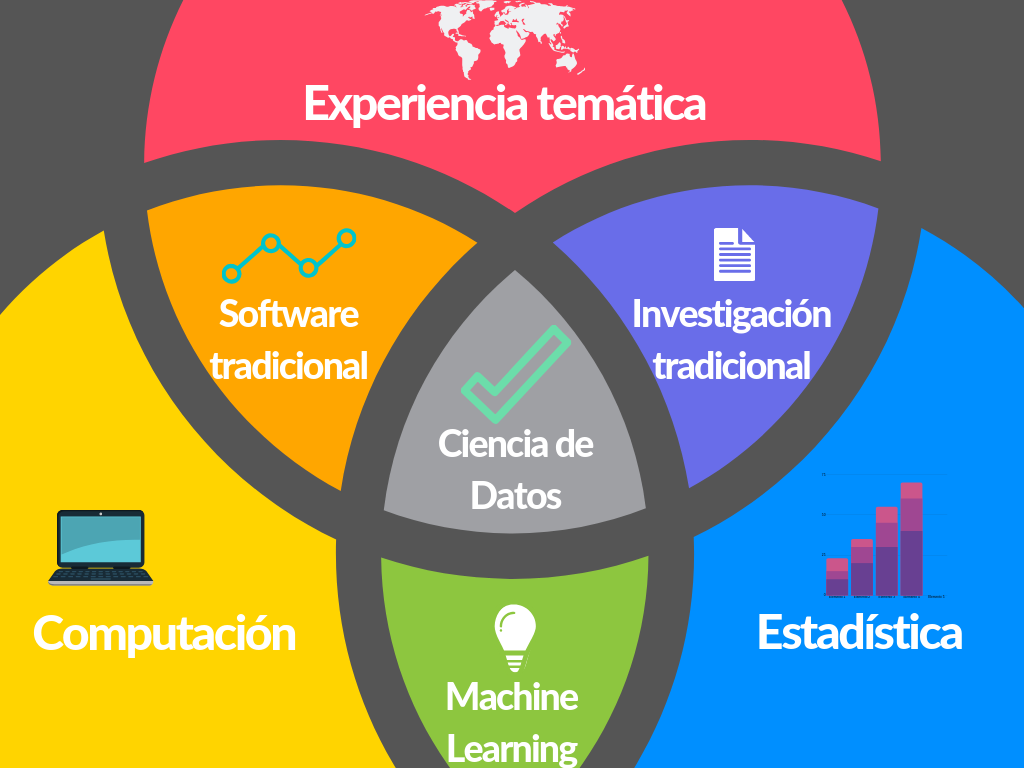
\includegraphics[width=10.41667in,height=\textheight]{img/venn_ds.png}

\hypertarget{presentacion}{%
\subsection*{Presentación}\label{presentacion}}
\addcontentsline{toc}{subsection}{Presentación}

En los últimos años se han difundido muchas herramientas estadísticas novedosas para el análisis de información socioeconómica y geográfica. En particular el software denominado ``R'', por tratarse de un software libre, se extiende cada vez más en diferentes disciplinas y recibe el aporte de investigadores e investigadoras en todo el mundo, multiplicando sistemáticamente sus capacidades.

Este programa se destaca, entre otras cosas, por su capacidad de trabajar con grandes volúmenes de información, utilizar múltiples bases de datos en simultáneo, generar reportes, realizar gráficos a nivel de publicación y por su comunidad de usuarios que publican sus sintaxis y comparten sus problemas, hecho que potencia la capacidad de consulta y de crecimiento. A su vez, la expresividad del lenguaje permite diseñar funciones específicas que permiten optimizar de forma personalizada el trabajo cotidiano con R.

\hypertarget{objetivos-del-curso}{%
\subsection*{Objetivos del curso}\label{objetivos-del-curso}}
\addcontentsline{toc}{subsection}{Objetivos del curso}

El presente Taller tiene como objetivo principal introducir a los participantes en la ciencia de datos, sobre la base de la utilización del lenguaje R aplicado procesamiento de diferentes bases de datos provistas por el programa de Gobierno Abierto y la Encuesta Permanente de Hogares (EPH) - INDEC. Se apunta a brindar las herramientas necesarias para la gestión de la información, presentación de resultados y algunas técnicas de modelado de datos, de forma tal que los participantes puedan luego avanzar por su cuenta a técnicas más avanzadas.

\hypertarget{webpage}{%
\subsection*{\texorpdfstring{\href{https://diegokoz.github.io/intro_ds/}{Webpage}}{Webpage}}\label{webpage}}
\addcontentsline{toc}{subsection}{\href{https://diegokoz.github.io/intro_ds/}{Webpage}}

\hypertarget{temario}{%
\subsection*{Temario:}\label{temario}}
\addcontentsline{toc}{subsection}{Temario:}

\hypertarget{eje-1.-programacion-en-r}{%
\subsubsection*{\texorpdfstring{\textbf{Eje 1. Programación en R}}{Eje 1. Programación en R}}\label{eje-1.-programacion-en-r}}
\addcontentsline{toc}{subsubsection}{\textbf{Eje 1. Programación en R}}

\textbf{clase 1}: Introducción al entorno R:

\begin{itemize}
\tightlist
\item
  Descripción del programa ``R''. Lógica sintáctica del lenguaje y comandos básicos
\item
  Presentación de la plataforma RStudio para trabajar en ``R''
\item
  Caracteres especiales en ``R''
\item
  Operadores lógicos y aritméticos
\item
  Definición de Objetos: Valores, Vectores y DataFrames
\item
  Tipos de variable (numérica, de caracteres, lógicas)
\item
  Lectura y Escritura de Archivos
\end{itemize}

\textbf{clase 2}: Tidyverse:

\begin{itemize}
\tightlist
\item
  Limpieza de Base de datos: Renombrar y recodificar variables, tratamiento de valores faltantes (missing values/ NA´s)
\item
  Seleccionar variables, ordenar y agrupar la base de datos para realizar cálculos
\item
  Creación de nuevas variables
\item
  Aplicar filtros sobre la base de datos
\item
  Construir medidas de resumen de la información
\item
  Tratamiento de variables numéricas (edad, ingresos, horas de trabajo, cantidad de hijos / componentes del hogar, entre otras).
\end{itemize}

\textbf{clase 3}: Programación funcional

\begin{itemize}
\tightlist
\item
  Estructuras de código condicionales
\item
  Loops
\item
  Creación de funciones a medida del usuario
\item
  Librería purrr para programación funcional
\end{itemize}

\hypertarget{eje-2.-presentacion-de-resultados}{%
\subsubsection*{\texorpdfstring{\textbf{Eje 2. Presentación de resultados}}{Eje 2. Presentación de resultados}}\label{eje-2.-presentacion-de-resultados}}
\addcontentsline{toc}{subsubsection}{\textbf{Eje 2. Presentación de resultados}}

\textbf{clase 4}: Visualización de la información

\begin{itemize}
\tightlist
\item
  Gráficos básicos de R (función ``plot''): Comandos para la visualización ágil de la información
\item
  Gráficos elaborados en R (función ``ggplot''):
\item
  Gráficos de línea, barras, Boxplots y distribuciones de densidad
\item
  Parámetros de los gráficos: Leyendas, ejes, títulos, notas, colores
\item
  Gráficos con múltiples cruces de variables.
\end{itemize}

\textbf{clase 5}: Documentación en R

\begin{itemize}
\tightlist
\item
  Manejo de las extensiones del software ``Rmarkdown'' y ``RNotebook'' para elaborar documentos de trabajo, presentaciones interactivas e informes:
\item
  Opciones para mostrar u ocultar código en los reportes
\item
  Definición de tamaño, títulos y formato con el cual se despliegan los gráficos y tablas en el informe
\item
  Caracteres especiales para incluir múltiples recursos en el texto del informe: Links a páginas web, notas al pie, enumeraciones, cambios en el formato de letra (tamaño, negrita, cursiva)
\item
  Código embebido en el texto para automatización de reportes
\end{itemize}

\textbf{clase 6}: Shiny

\begin{itemize}
\tightlist
\item
  Shiny como reportes dinámicos
\item
  Su utilidad para el análisis exploratorio
\item
  Lógica de servidor- interfaz de usuario
\item
  Extensiones del mundo shiny
\item
  Publicación de resultados
\end{itemize}

\hypertarget{eje-3.-estadistica}{%
\subsubsection*{\texorpdfstring{\textbf{Eje 3. Estadística}}{Eje 3. Estadística}}\label{eje-3.-estadistica}}
\addcontentsline{toc}{subsubsection}{\textbf{Eje 3. Estadística}}

\textbf{clase 7}: Estadística descriptiva

\begin{itemize}
\tightlist
\item
  Introducción a probabilidad
\item
  Introducción a distribuciones
\item
  El problema de la inversión
\item
  Estadística
\item
  Población y muestra
\item
  Estimadores puntuales, tests de hipótesis
\item
  Boxplots, histogramas y kernels
\end{itemize}

\textbf{clase 8}: Correlación y Modelo Lineal

\begin{itemize}
\tightlist
\item
  Análisis de correlación.
\item
  Presentación conceptual del modelo lineal
\item
  El modelo lineal desde una perspectiva computacional
\item
  Supuestos del modelo lineal
\item
  Modelo lineal en R
\item
  Modelo lineal en el tidyverse
\end{itemize}

\hypertarget{eje-4.-clases-tematicas}{%
\subsubsection*{\texorpdfstring{\textbf{Eje 4. Clases temáticas}}{Eje 4. Clases temáticas}}\label{eje-4.-clases-tematicas}}
\addcontentsline{toc}{subsubsection}{\textbf{Eje 4. Clases temáticas}}

\textbf{clase 9}: Análisis de encuestas

\begin{itemize}
\tightlist
\item
  Introducción al diseño de encuestas
\item
  Presentación de la Encuesta Permanente de Hogares
\item
  Generación de estadísticos de resumen en muestras estratificadas
\item
  Utilización de los ponderadores
\end{itemize}

\textbf{clase 10}: Mapas

\begin{itemize}
\tightlist
\item
  Utilización de información geográfica en R
\item
  Elaboración de mapas
\item
  gestión de shapefiles
\end{itemize}

\textbf{clase 11}: Text Mining

\begin{itemize}
\tightlist
\item
  Introducción al análisis de textos
\item
  Limpieza
\item
  Preprocesamiento
\item
  BoW
\item
  Stopwords
\item
  TF-IDF
\item
  Wordcloud
\item
  Escrapeo de Twitter
\end{itemize}

\hypertarget{bibliografia-de-consulta}{%
\subsection*{Bibliografía de consulta}\label{bibliografia-de-consulta}}
\addcontentsline{toc}{subsection}{Bibliografía de consulta}

\begin{itemize}
\tightlist
\item
  GWickham, H., \& Grolemund, G. (2016). R for data science: import, tidy, transform, visualize, and model data. " O'Reilly Media, Inc.". \url{https://es.r4ds.hadley.nz/}
\item
  James, G., Witten, D., Hastie, T., \& Tibshirani, R. (2013). An introduction to statistical learning. New York: springer. \url{http://faculty.marshall.usc.edu/gareth-james/ISL/}
\item
  Wickham, Hadley. ggplot2: elegant graphics for data analysis. Springer, 2016. \url{https://ggplot2-book.org/}
\end{itemize}

\hypertarget{librerias-a-instalar}{%
\subsubsection*{Librerias a instalar}\label{librerias-a-instalar}}
\addcontentsline{toc}{subsubsection}{Librerias a instalar}

\begin{verbatim}
install.packages(c("tidyverse","openxlsx","xlsx",'ggplot2','GGally','ggridges','treemapify','esquisse','cowplot','ggthemes', 'ggrepel', 'ggalt', 'kableExtra', 'fs', 'purrr', 'rmarkdown', 'modelr', 'plot3D'))
\end{verbatim}

\hypertarget{introduccion-a-r}{%
\chapter{Introducción a R}\label{introduccion-a-r}}

En esta primera clase revisaremos los fundamentos de R base y el entorno de RStudio. El objetivo es poder comenzar a utilizar el programa, abrir archivos y empezar a experimentar para ganar confianza.

\begin{itemize}
\tightlist
\item
  Descripción del programa \emph{R}. Lógica sintáctica del lenguaje y comandos básicos
\item
  Presentación de la plataforma RStudio para trabajar en \emph{R}
\item
  Caracteres especiales en \emph{R}
\item
  Operadores lógicos y aritméticos
\item
  Definición de objetos: valores, vectores y DataFrames
\item
  Tipos de variable (numéricas, de caracteres, lógicas)
\item
  Lectura y escritura de archivos
\end{itemize}

\hypertarget{explicacion}{%
\section{Explicación}\label{explicacion}}

\begin{figure}
\centering

\includegraphics[width=10.41667in,height=\textheight]{img/Rlogo.png}
\caption{\url{https://cran.r-project.org/}}
\end{figure}

\hypertarget{que-es-r}{%
\subsection{¿Qué es R?}\label{que-es-r}}

\begin{itemize}
\tightlist
\item
  Lenguaje para el procesamiento y análisis estadístico de datos
\item
  Software Libre
\item
  Sintaxis Básica: R base
\item
  Sintaxis incremental\footnote{Más allá de los comandos elementales, comandos más sofisticados tienen muchas versiones, y algunas quedan en desuso en el tiempo.}: El lenguaje se va ampliando por aportes de Universidades, investigadores/as, usuarios/as y empresas privadas, organizados en librerías (o paquetes)
\item
  Comunidad web muy grande para realizar preguntas y despejar dudas. Por ejemplo, en el caso de Buenos Aires contamos con \href{https://www.meetup.com/es-ES/rladies-buenos-aires/}{R-Ladies Buenos Aires} y \href{https://www.meetup.com/es-ES/renbaires/}{RenBaires}.
\item
  Gráficos con calidad de publicación
\end{itemize}

\begin{figure}
\centering
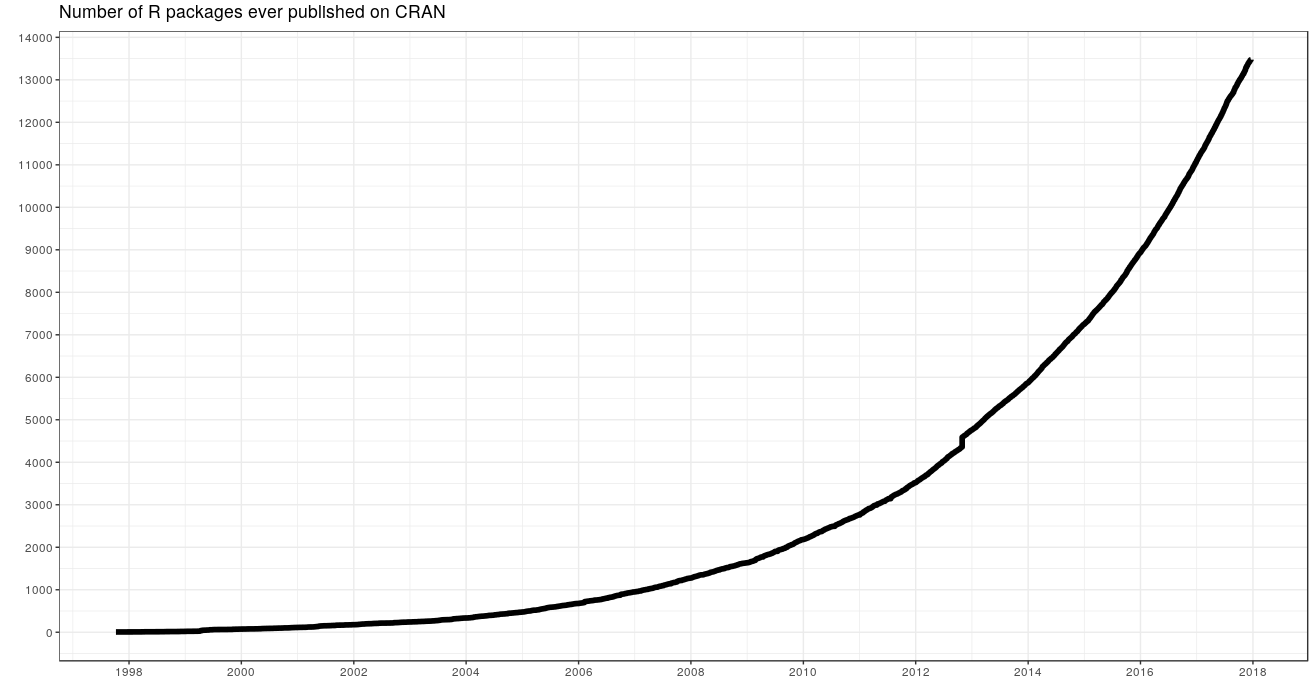
\includegraphics[width=10.41667in,height=\textheight]{img/number-of-submitted-packages-to-CRAN.png}
\caption{fuente: \url{https://gist.github.com/daroczig/3cf06d6db4be2bbe3368}}
\end{figure}

\begin{figure}
\centering

\includegraphics[width=10.41667in,height=\textheight]{img/RStudio-Logo-Flat.png}
\caption{\url{https://www.rstudio.com/}}
\end{figure}

Uno de los \emph{entornos} más cómodos para utilizar el \emph{lenguaje} \textbf{R} es el \emph{programa} \textbf{R studio}.

\begin{itemize}
\item
  Rstudio es una empresa que produce productos asociados al lenguaje R, como el programa sobre el que corremos los comandos, y extensiones del lenguaje (librerías).
\item
  El programa es \emph{gratuito} y se puede bajar de la
  \href{https://www.rstudio.com/}{página oficial}
\end{itemize}

\begin{figure}
\centering
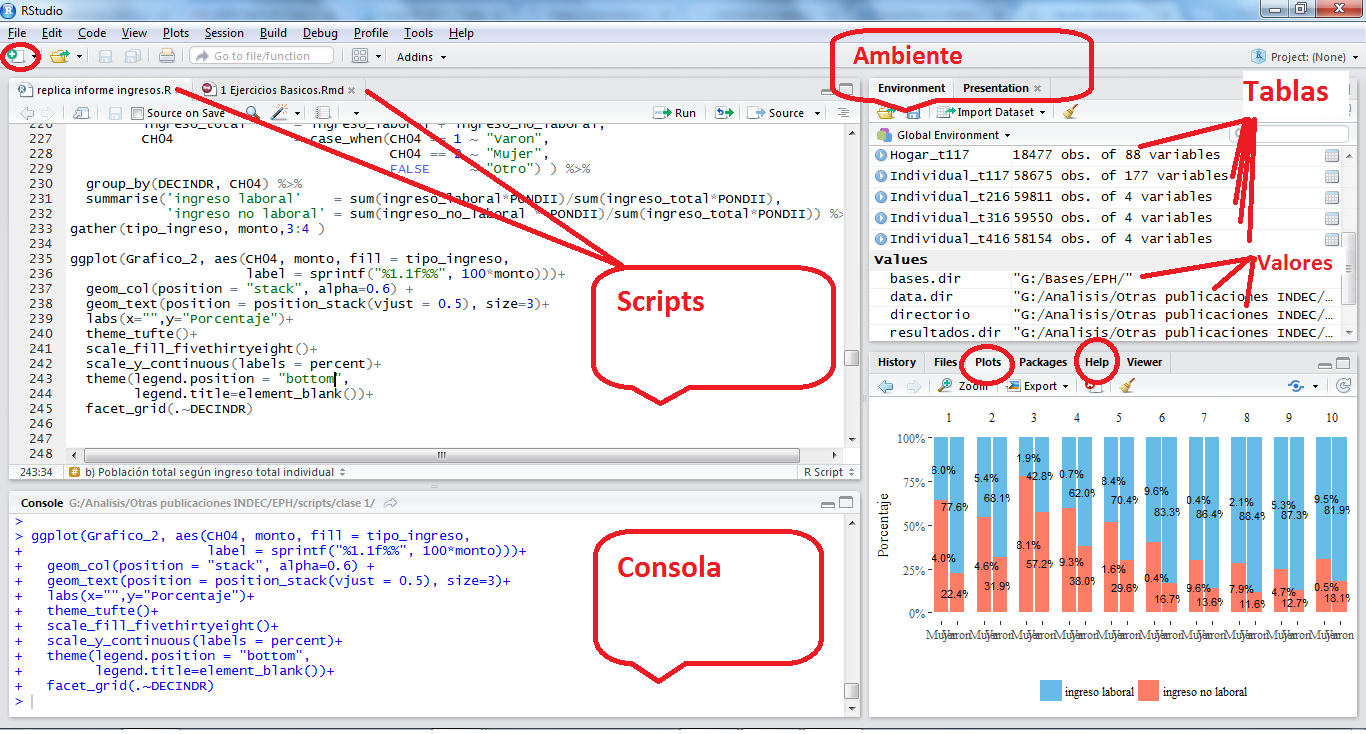
\includegraphics[width=10.41667in,height=\textheight]{img/Pantalla Rstudio.png}
\caption{Pantalla Rstudio}
\end{figure}

\hypertarget{logica-sintactica.}{%
\subsection{Lógica sintáctica.}\label{logica-sintactica.}}

\hypertarget{definicion-de-objetos}{%
\subsubsection{Definición de objetos}\label{definicion-de-objetos}}

Los \textbf{Objetos/Elementos} constituyen la categoría esencial del R. De hecho, todo en R es un objeto, y se almacena con un nombre específico que \textbf{no debe poseer espacios}. Un número, un vector, una función, la progresión de letras del abecedario, una base de datos, un gráfico, constituyen para R objetos de distinto tipo. Los objetos que vamos creando a medida que trabajamos pueden visualizarse en el panel derecho superior de la pantalla (el \emph{Environment}).

El operador \textbf{\texttt{\textless{}-}} (\textbf{Alt + Guión}) sirve para definir un objeto. \textbf{A la izquierda} del \textbf{\texttt{\textless{}-}} debe ubicarse el nombre que tomará el elemento a crear. \textbf{Del lado derecho} debe ir la definición del mismo.

\begin{Shaded}
\begin{Highlighting}[]
\NormalTok{A <-}\StringTok{ }\DecValTok{1}
\end{Highlighting}
\end{Shaded}

Por ejemplo, podemos crear el elemento \textbf{A}, cuyo valor será 1. Para esto, debemos \emph{correr} el código presionando \textbf{Ctrl + Enter}, con el cursor ubicado en cualquier parte de la línea. Al definir un elemento, el mismo queda guardado en el ambiente del programa, y podrá ser utilizado posteriormente para observar su contenido o para realizar una operación con el mismo.

\begin{Shaded}
\begin{Highlighting}[]
\NormalTok{A }
\end{Highlighting}
\end{Shaded}

\begin{verbatim}
## [1] 1
\end{verbatim}

\begin{Shaded}
\begin{Highlighting}[]
\NormalTok{A}\OperatorTok{+}\DecValTok{6}
\end{Highlighting}
\end{Shaded}

\begin{verbatim}
## [1] 7
\end{verbatim}

Al correr una linea con el nombre del objeto, la consola del programa nos muestra su contenido. Entre corchetes observamos el número de orden del elemento en cuestión. Si corremos una operación, la consola nos muestra el resultado de la misma.

El operador \textbf{\texttt{=}} es \textbf{equivalente} a \textbf{\texttt{\textless{}-}}, pero en la práctica no se utiliza para la definición de objetos.

\begin{Shaded}
\begin{Highlighting}[]
\NormalTok{B =}\StringTok{ }\DecValTok{2}
\NormalTok{B}
\end{Highlighting}
\end{Shaded}

\begin{verbatim}
## [1] 2
\end{verbatim}

\textbf{\texttt{\textless{}-}} es un operador \textbf{Unidireccional}, es decir que:\\
\texttt{A\ \textless{}-\ B} implica que \textbf{A} va tomar como valor el contenido del objeto \textbf{B}, y no al revés.

\begin{Shaded}
\begin{Highlighting}[]
\NormalTok{A <-}\StringTok{ }\NormalTok{B}
\NormalTok{A      }\CommentTok{# Ahora A toma el valor de B, y B continúa conservando el mismo valor}
\end{Highlighting}
\end{Shaded}

\begin{verbatim}
## [1] 2
\end{verbatim}

\begin{Shaded}
\begin{Highlighting}[]
\NormalTok{B}
\end{Highlighting}
\end{Shaded}

\begin{verbatim}
## [1] 2
\end{verbatim}

\hypertarget{r-base}{%
\subsection{R base}\label{r-base}}

Con \emph{R base} nos referimos a los comandos básicos que vienen incorporados en el R, sin necesidad de cargar librerías.

\hypertarget{operadores-logicos}{%
\subsubsection{Operadores lógicos:}\label{operadores-logicos}}

\begin{itemize}
\tightlist
\item
  \(>\) (mayor a-)
\item
  \(>=\) (mayor o igual a-)
\item
  \(<\) (menor a-)
\item
  \(<=\) (menor o igual a-)
\item
  \(==\) (igual a-)
\item
  \(!=\) (distinto a-)
\end{itemize}

\begin{Shaded}
\begin{Highlighting}[]
\CommentTok{# Redefinimos los valores A y B}
\NormalTok{A <-}\StringTok{ }\DecValTok{10}
\NormalTok{B <-}\StringTok{ }\DecValTok{20}

\CommentTok{# Realizamos comparaciones lógicas}
\NormalTok{A }\OperatorTok{>}\StringTok{  }\NormalTok{B}
\end{Highlighting}
\end{Shaded}

\begin{verbatim}
## [1] FALSE
\end{verbatim}

\begin{Shaded}
\begin{Highlighting}[]
\NormalTok{A }\OperatorTok{>=}\StringTok{ }\NormalTok{B}
\end{Highlighting}
\end{Shaded}

\begin{verbatim}
## [1] FALSE
\end{verbatim}

\begin{Shaded}
\begin{Highlighting}[]
\NormalTok{A }\OperatorTok{<}\StringTok{  }\NormalTok{B}
\end{Highlighting}
\end{Shaded}

\begin{verbatim}
## [1] TRUE
\end{verbatim}

\begin{Shaded}
\begin{Highlighting}[]
\NormalTok{A }\OperatorTok{<=}\StringTok{ }\NormalTok{B}
\end{Highlighting}
\end{Shaded}

\begin{verbatim}
## [1] TRUE
\end{verbatim}

\begin{Shaded}
\begin{Highlighting}[]
\NormalTok{A }\OperatorTok{==}\StringTok{ }\NormalTok{B}
\end{Highlighting}
\end{Shaded}

\begin{verbatim}
## [1] FALSE
\end{verbatim}

\begin{Shaded}
\begin{Highlighting}[]
\NormalTok{A }\OperatorTok{!=}\StringTok{ }\NormalTok{B}
\end{Highlighting}
\end{Shaded}

\begin{verbatim}
## [1] TRUE
\end{verbatim}

\begin{Shaded}
\begin{Highlighting}[]
\NormalTok{C <-}\StringTok{ }\NormalTok{A }\OperatorTok{!=}\StringTok{ }\NormalTok{B}
\NormalTok{C}
\end{Highlighting}
\end{Shaded}

\begin{verbatim}
## [1] TRUE
\end{verbatim}

Como muestra el último ejemplo, el resultado de una operación lógica puede almacenarse como el valor de un objeto.

\hypertarget{operadores-aritmeticos}{%
\subsubsection{Operadores aritméticos:}\label{operadores-aritmeticos}}

\begin{Shaded}
\begin{Highlighting}[]
\CommentTok{#suma}
\NormalTok{A <-}\StringTok{ }\DecValTok{5}\OperatorTok{+}\DecValTok{6}
\NormalTok{A}
\end{Highlighting}
\end{Shaded}

\begin{verbatim}
## [1] 11
\end{verbatim}

\begin{Shaded}
\begin{Highlighting}[]
\CommentTok{#Resta}
\NormalTok{B <-}\StringTok{ }\DecValTok{6-8}
\NormalTok{B}
\end{Highlighting}
\end{Shaded}

\begin{verbatim}
## [1] -2
\end{verbatim}

\begin{Shaded}
\begin{Highlighting}[]
\CommentTok{#cociente}
\NormalTok{C <-}\StringTok{ }\DecValTok{6}\OperatorTok{/}\FloatTok{2.5}
\NormalTok{C}
\end{Highlighting}
\end{Shaded}

\begin{verbatim}
## [1] 2.4
\end{verbatim}

\begin{Shaded}
\begin{Highlighting}[]
\CommentTok{#multiplicacion}
\NormalTok{D <-}\StringTok{ }\DecValTok{6}\OperatorTok{*}\FloatTok{2.5}
\NormalTok{D}
\end{Highlighting}
\end{Shaded}

\begin{verbatim}
## [1] 15
\end{verbatim}

\hypertarget{funciones}{%
\subsubsection{Funciones:}\label{funciones}}

Las funciones son series de procedimientos estandarizados, que toman como imput determinados argumentos a fijar por el usuario, y devuelven un resultado acorde a la aplicación de dichos procedimientos. Su lógica de funcionamiento es:\\
\texttt{funcion(argumento1\ =\ arg1,\ argumento2\ =\ arg2)}

A lo largo del curso iremos viendo numerosas funciones, según lo requieran los distintos ejercicios. Sin embargo, veamos ahora algunos ejemplos para comprender su funcionamiento:

\begin{itemize}
\tightlist
\item
  paste() : concatena una serie de caracteres, pudiendo indicarse cómo separar a cada uno de ellos\\
\item
  paste0(): concatena una serie de caracteres sin separar
\item
  sum(): suma de todos los elementos de un vector\\
\item
  mean() promedio aritmético de todos los elementos de un vector
\end{itemize}

\begin{Shaded}
\begin{Highlighting}[]
\KeywordTok{paste}\NormalTok{(}\StringTok{"Pega"}\NormalTok{, }\StringTok{"estas"}\NormalTok{, }\DecValTok{4}\NormalTok{, }\StringTok{"palabras"}\NormalTok{, }\DataTypeTok{sep =} \StringTok{" "}\NormalTok{)}
\end{Highlighting}
\end{Shaded}

\begin{verbatim}
## [1] "Pega estas 4 palabras"
\end{verbatim}

\begin{Shaded}
\begin{Highlighting}[]
\CommentTok{#Puedo concatenar caracteres almacenados en objetos}
\KeywordTok{paste}\NormalTok{(A, B, C, }\DataTypeTok{sep =} \StringTok{"**"}\NormalTok{)}
\end{Highlighting}
\end{Shaded}

\begin{verbatim}
## [1] "11**-2**2.4"
\end{verbatim}

\begin{Shaded}
\begin{Highlighting}[]
\CommentTok{# Paste0 pega los caracteres sin separador}
\KeywordTok{paste0}\NormalTok{(A, B, C)}
\end{Highlighting}
\end{Shaded}

\begin{verbatim}
## [1] "11-22.4"
\end{verbatim}

\begin{Shaded}
\begin{Highlighting}[]
\DecValTok{1}\OperatorTok{:}\DecValTok{5}
\end{Highlighting}
\end{Shaded}

\begin{verbatim}
## [1] 1 2 3 4 5
\end{verbatim}

\begin{Shaded}
\begin{Highlighting}[]
\KeywordTok{sum}\NormalTok{(}\DecValTok{1}\OperatorTok{:}\DecValTok{5}\NormalTok{)}
\end{Highlighting}
\end{Shaded}

\begin{verbatim}
## [1] 15
\end{verbatim}

\begin{Shaded}
\begin{Highlighting}[]
\KeywordTok{mean}\NormalTok{(}\DecValTok{1}\OperatorTok{:}\DecValTok{5}\NormalTok{, }\DataTypeTok{na.rm =} \OtherTok{TRUE}\NormalTok{)}
\end{Highlighting}
\end{Shaded}

\begin{verbatim}
## [1] 3
\end{verbatim}

\hypertarget{caracteres-especiales}{%
\subsubsection{Caracteres especiales}\label{caracteres-especiales}}

\begin{itemize}
\tightlist
\item
  R es sensible a mayúsculas y minúsculas, tanto para los nombres de las variables, como para las funciones y parámetros.
\item
  Los \textbf{espacios en blanco} y los \textbf{carriage return} (\emph{enter}) no son considerados por el lenguaje. Los podemos aprovechar para emprolijar el código y que la lectura sea más simple\footnote{veremos que existen ciertas excepciones con algunos paquetes más adelante.}.
\end{itemize}

\begin{itemize}
\item
  El \textbf{numeral} \texttt{\#} se utiliza para hacer comentarios. Todo lo que se escribe después del \# no es interpretado por R. Se debe utilizar un \# por cada línea de código que se desea anular
\item
  Los \textbf{corchetes} \texttt{{[}{]}} se utilizan para acceder a un objeto:

  \begin{itemize}
  \tightlist
  \item
    en un vector{[}n° orden{]}
  \item
    en una tabla{[}fila, columna{]}
  \item
    en una lista{[}n° elemento{]}
  \end{itemize}
\item
  el signo \textbf{\$} también es un método de acceso. Particularmente, en los dataframes, nos permitira acceder a una determinada columna de una tabla
\item
  Los \textbf{paréntesis}\texttt{()} se utilizan en las funciones para definir los parámetros.
\item
  Las \textbf{comas} \texttt{,} se utilizan para separar los parametros al interior de una función.
\end{itemize}

\hypertarget{objetos}{%
\subsection{Objetos:}\label{objetos}}

Existe una gran cantidad de objetos distintos en R, en lo que resepcta al curso trabajaremos principalmente con 3 de ellos:

\begin{itemize}
\tightlist
\item
  Valores
\item
  Vectores
\item
  Data Frames
\item
  Listas
\end{itemize}

\hypertarget{valores}{%
\subsubsection{Valores}\label{valores}}

Los valores y vectores pueden ser a su vez de distintas \emph{clases}:

\textbf{Numeric}

\begin{Shaded}
\begin{Highlighting}[]
\NormalTok{A <-}\StringTok{  }\DecValTok{1}
\KeywordTok{class}\NormalTok{(A)}
\end{Highlighting}
\end{Shaded}

\begin{verbatim}
## [1] "numeric"
\end{verbatim}

\textbf{Character}

\begin{Shaded}
\begin{Highlighting}[]
\NormalTok{A <-}\StringTok{  }\KeywordTok{paste}\NormalTok{(}\StringTok{'Soy'}\NormalTok{, }\StringTok{'una'}\NormalTok{, }\StringTok{'concatenación', '}\NormalTok{de}\StringTok{', '}\NormalTok{caracteres}\StringTok{', sep = " ")}
\StringTok{A}
\end{Highlighting}
\end{Shaded}

\begin{verbatim}
## [1] "Soy una concatenación de caracteres"
\end{verbatim}

\begin{Shaded}
\begin{Highlighting}[]
\KeywordTok{class}\NormalTok{(A)}
\end{Highlighting}
\end{Shaded}

\begin{verbatim}
## [1] "character"
\end{verbatim}

\textbf{Factor}

\begin{Shaded}
\begin{Highlighting}[]
\NormalTok{A <-}\StringTok{ }\KeywordTok{factor}\NormalTok{(}\StringTok{"Soy un factor, con niveles fijos"}\NormalTok{)}
\KeywordTok{class}\NormalTok{(A)}
\end{Highlighting}
\end{Shaded}

\begin{verbatim}
## [1] "factor"
\end{verbatim}

La diferencia entre un \emph{character} y un \emph{factor} es que el último tiene solo algunos valores permitidos (levels), con un orden interno predefinido (el cual, por ejemplo, se respetará a la hora de realizar un gráfico)

\hypertarget{vectores}{%
\subsubsection{Vectores}\label{vectores}}

Para crear un \textbf{vector} utilizamos el comando \texttt{c()}, de combinar.

\begin{Shaded}
\begin{Highlighting}[]
\NormalTok{C <-}\StringTok{ }\KeywordTok{c}\NormalTok{(}\DecValTok{1}\NormalTok{, }\DecValTok{3}\NormalTok{, }\DecValTok{4}\NormalTok{)}
\NormalTok{C}
\end{Highlighting}
\end{Shaded}

\begin{verbatim}
## [1] 1 3 4
\end{verbatim}

Podemos sumarle 2 a cada elemento del \textbf{vector} anterior

\begin{Shaded}
\begin{Highlighting}[]
\NormalTok{C <-}\StringTok{ }\NormalTok{C }\OperatorTok{+}\StringTok{ }\DecValTok{2}
\NormalTok{C}
\end{Highlighting}
\end{Shaded}

\begin{verbatim}
## [1] 3 5 6
\end{verbatim}

O sumarle 1 al primer elemento, 2 al segundo, y 3 al tercer elemento del \textbf{vector} anterior

\begin{Shaded}
\begin{Highlighting}[]
\NormalTok{D <-}\StringTok{ }\NormalTok{C }\OperatorTok{+}\StringTok{ }\DecValTok{1}\OperatorTok{:}\DecValTok{3} \CommentTok{# esto es equivalente a hacer 3+1, 5+2, 6+9 }
\NormalTok{D}
\end{Highlighting}
\end{Shaded}

\begin{verbatim}
## [1] 4 7 9
\end{verbatim}

\texttt{1:3} significa que queremos todos los números enteros desde 1 hasta 3.

Podemos crear un \textbf{vector} que contenga las palabras: ``Carlos'', ``Federico'', ``Pedro''

\begin{Shaded}
\begin{Highlighting}[]
\NormalTok{E <-}\StringTok{ }\KeywordTok{c}\NormalTok{(}\StringTok{"Carlos"}\NormalTok{, }\StringTok{"Federico"}\NormalTok{, }\StringTok{"Pedro"}\NormalTok{)}
\NormalTok{E}
\end{Highlighting}
\end{Shaded}

\begin{verbatim}
## [1] "Carlos"   "Federico" "Pedro"
\end{verbatim}

Para acceder a algún elemento del vector, podemos buscarlo por su número de orden, entre \texttt{{[}\ {]}}

\begin{Shaded}
\begin{Highlighting}[]
\NormalTok{E[}\DecValTok{2}\NormalTok{]}
\end{Highlighting}
\end{Shaded}

\begin{verbatim}
## [1] "Federico"
\end{verbatim}

Si nos interesa almacenar dicho valor, al buscarlo lo asignamos a un nuevo objeto, dándole el nombre que deseemos

\begin{Shaded}
\begin{Highlighting}[]
\NormalTok{elemento2 <-}\StringTok{ }\NormalTok{E[}\DecValTok{2}\NormalTok{]}
\end{Highlighting}
\end{Shaded}

\begin{Shaded}
\begin{Highlighting}[]
\NormalTok{elemento2}
\end{Highlighting}
\end{Shaded}

\begin{verbatim}
## [1] "Federico"
\end{verbatim}

Para \textbf{borrar} un objeto del ambiente de trabajo, utilizamos el comando \emph{\texttt{rm()}}

\begin{Shaded}
\begin{Highlighting}[]
\KeywordTok{rm}\NormalTok{(elemento2)}
\NormalTok{elemento2}
\end{Highlighting}
\end{Shaded}

\begin{verbatim}
## Error in eval(expr, envir, enclos): object 'elemento2' not found
\end{verbatim}

También podemos cambiar el texto del segundo elemento de E, por el texto ``Pablo''

\begin{Shaded}
\begin{Highlighting}[]
\NormalTok{E[}\DecValTok{2}\NormalTok{] <-}\StringTok{ "Pablo"}
\NormalTok{E}
\end{Highlighting}
\end{Shaded}

\begin{verbatim}
## [1] "Carlos" "Pablo"  "Pedro"
\end{verbatim}

\hypertarget{data-frames}{%
\subsection{Data Frames}\label{data-frames}}

Un Data Frame es una tabla de datos, donde cada columna representa una variable, y cada fila una observación.

Este objeto suele ser central en el proceso de trabajo, y suele ser la forma en que se cargan datos externos para trabajar en el ambiente de R, y en que se exportan los resultados de nuestros trabajo.

También se puede crear como la combinación de N vectores de igual tamaño. Por ejemplo, tomamos algunos valores del \href{http://www.indec.gob.ar/bajarCuadroEstadistico.asp?idc=4020B33440609462654542BD0BC320F1523DA0DC52C396201DB4DD5861FFEDC9AD1436681AC84179}{Indice de salarios}

\begin{Shaded}
\begin{Highlighting}[]
\NormalTok{INDICE  <-}\StringTok{ }\KeywordTok{c}\NormalTok{(}\DecValTok{100}\NormalTok{,   }\DecValTok{100}\NormalTok{,   }\DecValTok{100}\NormalTok{,}
             \FloatTok{101.8}\NormalTok{, }\FloatTok{101.2}\NormalTok{, }\FloatTok{100.73}\NormalTok{,}
             \FloatTok{102.9}\NormalTok{, }\FloatTok{102.4}\NormalTok{, }\FloatTok{103.2}\NormalTok{)}

\NormalTok{FECHA  <-}\StringTok{  }\KeywordTok{c}\NormalTok{(}\StringTok{"Oct-16"}\NormalTok{, }\StringTok{"Oct-16"}\NormalTok{, }\StringTok{"Oct-16"}\NormalTok{,}
             \StringTok{"Nov-16"}\NormalTok{, }\StringTok{"Nov-16"}\NormalTok{, }\StringTok{"Nov-16"}\NormalTok{,}
             \StringTok{"Dic-16"}\NormalTok{, }\StringTok{"Dic-16"}\NormalTok{, }\StringTok{"Dic-16"}\NormalTok{)}

\NormalTok{GRUPO  <-}\StringTok{  }\KeywordTok{c}\NormalTok{(}\StringTok{"Privado_Registrado"}\NormalTok{,}\StringTok{"Público","}\NormalTok{Privado_No_Registrado}\StringTok{",}
\StringTok{             "}\NormalTok{Privado_Registrado}\StringTok{","}\NormalTok{Público",}\StringTok{"Privado_No_Registrado"}\NormalTok{,}
             \StringTok{"Privado_Registrado"}\NormalTok{,}\StringTok{"Público","}\NormalTok{Privado_No_Registrado}\StringTok{")}
\StringTok{             }
\StringTok{Datos <- data.frame(INDICE, FECHA, GRUPO)}
\StringTok{Datos}
\end{Highlighting}
\end{Shaded}

\begin{verbatim}
##   INDICE  FECHA                 GRUPO
## 1 100.00 Oct-16    Privado_Registrado
## 2 100.00 Oct-16               Público
## 3 100.00 Oct-16 Privado_No_Registrado
## 4 101.80 Nov-16    Privado_Registrado
## 5 101.20 Nov-16               Público
## 6 100.73 Nov-16 Privado_No_Registrado
## 7 102.90 Dic-16    Privado_Registrado
## 8 102.40 Dic-16               Público
## 9 103.20 Dic-16 Privado_No_Registrado
\end{verbatim}

Tal como en un \textbf{vector} se ubica a los elementos mediante \texttt{{[}\ {]}}, en un \textbf{dataframe} se obtienen sus elementos de la forma \textbf{\texttt{{[}fila,\ columna{]}}}.

Otra opción es especificar la columna, mediante el operador \textbf{\texttt{\$}}, y luego seleccionar dentro de esa columna el registro deseado mediante el número de orden.

\begin{Shaded}
\begin{Highlighting}[]
\NormalTok{Datos}\OperatorTok{$}\NormalTok{FECHA}
\end{Highlighting}
\end{Shaded}

\begin{verbatim}
## [1] Oct-16 Oct-16 Oct-16 Nov-16 Nov-16 Nov-16 Dic-16 Dic-16 Dic-16
## Levels: Dic-16 Nov-16 Oct-16
\end{verbatim}

\begin{Shaded}
\begin{Highlighting}[]
\NormalTok{Datos[}\DecValTok{3}\NormalTok{,}\DecValTok{2}\NormalTok{]}
\end{Highlighting}
\end{Shaded}

\begin{verbatim}
## [1] Oct-16
## Levels: Dic-16 Nov-16 Oct-16
\end{verbatim}

\begin{Shaded}
\begin{Highlighting}[]
\NormalTok{Datos}\OperatorTok{$}\NormalTok{FECHA[}\DecValTok{3}\NormalTok{]}
\end{Highlighting}
\end{Shaded}

\begin{verbatim}
## [1] Oct-16
## Levels: Dic-16 Nov-16 Oct-16
\end{verbatim}

¿que pasa si hacemos \texttt{Datos\$FECHA{[}3,2{]}} ?

\begin{Shaded}
\begin{Highlighting}[]
\NormalTok{Datos}\OperatorTok{$}\NormalTok{FECHA[}\DecValTok{3}\NormalTok{,}\DecValTok{2}\NormalTok{]}
\end{Highlighting}
\end{Shaded}

\begin{verbatim}
## Error in `[.default`(Datos$FECHA, 3, 2): incorrect number of dimensions
\end{verbatim}

Nótese que el último comando tiene un número incorrecto de dimensiones, porque estamos refiriendonos 2 veces a la columna FECHA.

Acorde a lo visto anteriormente, el acceso a los \textbf{dataframes} mediante \texttt{{[}\ {]}} puede utilizarse para realizar filtros sobre la base, especificando una condición para las filas. Por ejemplo, puedo utilizar los \texttt{{[}\ {]}} para conservar del \textbf{dataframe} \texttt{Datos} unicamente los registros con fecha de Diciembre 2016:

\begin{Shaded}
\begin{Highlighting}[]
\NormalTok{Datos[Datos}\OperatorTok{$}\NormalTok{FECHA}\OperatorTok{==}\StringTok{"Dic-16"}\NormalTok{,]}
\end{Highlighting}
\end{Shaded}

\begin{verbatim}
##   INDICE  FECHA                 GRUPO
## 7  102.9 Dic-16    Privado_Registrado
## 8  102.4 Dic-16               Público
## 9  103.2 Dic-16 Privado_No_Registrado
\end{verbatim}

La lógica del paso anterior sería: Accedo al dataframe \texttt{Datos}, pidiendo únicamente conservar las filas (por eso la condición se ubica a la \emph{izquierda} de la \texttt{,}) que cumplan el requisito de pertenecer a la categoría \textbf{``Dic-16''} de la variable \textbf{FECHA}.

Aún más, podría aplicar el filtro y al mismo tiempo identificar una variable de interés para luego realizar un cálculo sobre aquella. Por ejemplo, podría calcular la media de los indices en el mes de Diciembre.

\begin{Shaded}
\begin{Highlighting}[]
\CommentTok{###Por separado}
\NormalTok{Indices_Dic <-}\StringTok{ }\NormalTok{Datos}\OperatorTok{$}\NormalTok{INDICE[Datos}\OperatorTok{$}\NormalTok{FECHA}\OperatorTok{==}\StringTok{"Dic-16"}\NormalTok{]}
\NormalTok{Indices_Dic}
\end{Highlighting}
\end{Shaded}

\begin{verbatim}
## [1] 102.9 102.4 103.2
\end{verbatim}

\begin{Shaded}
\begin{Highlighting}[]
\KeywordTok{mean}\NormalTok{(Indices_Dic)}
\end{Highlighting}
\end{Shaded}

\begin{verbatim}
## [1] 102.8333
\end{verbatim}

\begin{Shaded}
\begin{Highlighting}[]
\CommentTok{### Todo junto}
\KeywordTok{mean}\NormalTok{(Datos}\OperatorTok{$}\NormalTok{INDICE[Datos}\OperatorTok{$}\NormalTok{FECHA}\OperatorTok{==}\StringTok{"Dic-16"}\NormalTok{])}
\end{Highlighting}
\end{Shaded}

\begin{verbatim}
## [1] 102.8333
\end{verbatim}

La lógica de esta sintaxis sería: ``Me quedo con la variable \textbf{INDICE}, cuando la variable FECHA sea igual a \textbf{"Dic-16"}, luego calculo la media de dichos valores''.

\hypertarget{listas}{%
\subsection{Listas}\label{listas}}

Contienen una concatenación de objetos de cualquier tipo. Así como un vector contiene valores, un dataframe contiene vectores, una lista puede contener dataframes, pero también vectores, o valores, y \emph{todo ello a la vez}.

\begin{Shaded}
\begin{Highlighting}[]
\NormalTok{superlista <-}\StringTok{ }\KeywordTok{list}\NormalTok{(A,B,C,D,E,FECHA, }\DataTypeTok{DF =}\NormalTok{ Datos, INDICE, GRUPO)}
\NormalTok{superlista}
\end{Highlighting}
\end{Shaded}

\begin{verbatim}
## [[1]]
## [1] Soy un factor, con niveles fijos
## Levels: Soy un factor, con niveles fijos
## 
## [[2]]
## [1] -2
## 
## [[3]]
## [1] 3 5 6
## 
## [[4]]
## [1] 4 7 9
## 
## [[5]]
## [1] "Carlos" "Pablo"  "Pedro" 
## 
## [[6]]
## [1] "Oct-16" "Oct-16" "Oct-16" "Nov-16" "Nov-16" "Nov-16" "Dic-16" "Dic-16"
## [9] "Dic-16"
## 
## $DF
##   INDICE  FECHA                 GRUPO
## 1 100.00 Oct-16    Privado_Registrado
## 2 100.00 Oct-16               Público
## 3 100.00 Oct-16 Privado_No_Registrado
## 4 101.80 Nov-16    Privado_Registrado
## 5 101.20 Nov-16               Público
## 6 100.73 Nov-16 Privado_No_Registrado
## 7 102.90 Dic-16    Privado_Registrado
## 8 102.40 Dic-16               Público
## 9 103.20 Dic-16 Privado_No_Registrado
## 
## [[8]]
## [1] 100.00 100.00 100.00 101.80 101.20 100.73 102.90 102.40 103.20
## 
## [[9]]
## [1] "Privado_Registrado"    "Público"               "Privado_No_Registrado"
## [4] "Privado_Registrado"    "Público"               "Privado_No_Registrado"
## [7] "Privado_Registrado"    "Público"               "Privado_No_Registrado"
\end{verbatim}

Para acceder un elemento de una lista, podemos utilizar el operador \textbf{\texttt{\$}}, que se puede usar a su vez de forma iterativa.

\begin{Shaded}
\begin{Highlighting}[]
\NormalTok{superlista}\OperatorTok{$}\NormalTok{DF}\OperatorTok{$}\NormalTok{FECHA[}\DecValTok{2}\NormalTok{]}
\end{Highlighting}
\end{Shaded}

\begin{verbatim}
## [1] Oct-16
## Levels: Dic-16 Nov-16 Oct-16
\end{verbatim}

\hypertarget{ambientes-de-trabajo}{%
\subsection{Ambientes de trabajo}\label{ambientes-de-trabajo}}

Hay algunas cosas que tenemos que tener en cuenta respecto del orden del ambiente en el que trabajamos:

\begin{itemize}
\tightlist
\item
  Working Directory: Es el directorio de trabajo. Pueden ver el suyo con \texttt{getwd()}, es \emph{hacia donde apunta el código}, por ejemplo, si quieren leer un archivo, la ruta del archivo tiene que estar explicitada como el recorrido desde el Working Directory.
\item
  Environment: Esto engloba tanto la información que tenemos cargada en \emph{Data} y \emph{Values}, como las librerías que tenemos cargadas mientras trabajamos.
\end{itemize}

Es importante que mantengamos bien delimitadas estas cosas entre diferentes trabajos, sino:

\begin{enumerate}
\def\labelenumi{\arabic{enumi}.}
\tightlist
\item
  El directorio queda referido a un lugar específico en nuestra computadora.
\end{enumerate}

\begin{itemize}
\tightlist
\item
  Si se lo compartimos a otro \textbf{se rompe}
\item
  Si cambiamos de computadora \textbf{se rompe}
\item
  Si lo cambiamos de lugar \textbf{se rompe}
\item
  Si primero abrimos otro script \textbf{se rompe}
\end{itemize}

\begin{enumerate}
\def\labelenumi{\arabic{enumi}.}
\setcounter{enumi}{1}
\tightlist
\item
  Tenemos mezclados resultados de diferentes trabajos:
\end{enumerate}

\begin{itemize}
\tightlist
\item
  Nunca sabemos si esa variable/tabla/lista se creo en ese script y no otro
\item
  Perdemos espacio de la memoria
\item
  No estamos seguros de que el script cargue todas las librerías que necesita
\end{itemize}

Rstudio tiene una herramienta muy útil de trabajo que son los \textbf{proyectos}. Estos permiten mantener un ambiente de trabajo delimitado por cada uno de nuestros trabajos. Es decir:

\begin{itemize}
\tightlist
\item
  El directorio de trabajo se refiere a donde esta ubicado el archivo .Rproj
\item
  El Environment es específico de nuestro proyecto.
\end{itemize}

Un proyecto no es un sólo script, sino toda una carpeta de trabajo.

\begin{figure}
\centering

\includegraphics[width=10.41667in,height=\textheight]{img/Rproject.png}
\caption{logo Rpoject}
\end{figure}

Para crearlo, vamos al logo de nuevo projecto (Arriba a la derecha de la panatalla), y elegimos la carpeta de trabajo.

\hypertarget{tipos-de-archivos-de-r}{%
\subsection{Tipos de archivos de R}\label{tipos-de-archivos-de-r}}

\begin{itemize}
\tightlist
\item
  \textbf{Script}: Es un archivo de texto plano, donde podemos poner el código que utilizamos para preservarlo
\item
  \textbf{Rnotebook}: También sirve para guardar el código, pero a diferencia de los scripts, se puede compilar, e intercalar código con resultados
\item
  \textbf{Rproject}: Es un archivo que define la metadata del proyecto
\item
  \textbf{RDS y Rdata}: Dos formatos de archivos propios de R para guardar datos.
\end{itemize}

\hypertarget{practica-guiada}{%
\section{Práctica Guiada}\label{practica-guiada}}

\hypertarget{instalacion-de-paquetes-complementarios-al-r-base}{%
\subsection{Instalación de paquetes complementarios al R Base}\label{instalacion-de-paquetes-complementarios-al-r-base}}

Hasta aquí hemos visto múltiples funciones que están contenidas dentro del lenguaje básico de R. Ahora bien, al tratarse de un software libre, los usuarios de R con más experiencia contribuyen sistemáticamente a expandir este lenguaje mediante la creación y actualización de \textbf{paquetes} complementarios. Lógicamente, los mismos no están incluidos en la instalación inicial del programa, pero podemos descargarlos e instalarlos al mismo tiempo con el siguiente comando:

\begin{verbatim}
install.packages("nombre_del_paquete") 
\end{verbatim}

Resulta recomendable \textbf{ejecutar este comando desde la consola} ya que sólo necesitaremos correrlo una vez en nuestra computadora. Al ejecutar el mismo, se descargarán de la pagina de \href{www.cran.r-project.org}{CRAN} los archivos correspondientes al paquete hacia el directorio en donde hayamos instalado el programa. Típicamente los archivos se encontrarán en \textbf{\texttt{C:\textbackslash{}Program\ Files\textbackslash{}R\textbackslash{}R-3.5.0\textbackslash{}library\textbackslash{}}}, siempre con la versión del programa correspondiente.\\
Una vez instalado el paquete, cada vez que abramos una nueva sesión de R y querramos utilizar el mismo debemos \textbf{cargarlo al ambiente de trabajo} mediante la siguiente función:

\begin{verbatim}
library(nombre_del_paquete)
\end{verbatim}

Nótese que al cargar/activar el paquete no son necesarias las comillas.

\hypertarget{lectura-y-escritura-de-archivos}{%
\subsection{Lectura y escritura de archivos}\label{lectura-y-escritura-de-archivos}}

\hypertarget{csv-y-.txt}{%
\subsubsection{.csv y .txt}\label{csv-y-.txt}}

Hay \textbf{muchas} funciones para leer archivos de tipo \emph{.txt} y \emph{.csv}. La mayoría sólo cambia los parámetros que vienen por default.

Es importante tener en cuenta que una base de datos que proviene de archivos \emph{.txt}, o \emph{.csv} puede presentar diferencias en cuanto a los siguientes parámetros:

\begin{itemize}
\tightlist
\item
  encabezado
\item
  delimitador (\texttt{,}, tab, \texttt{;})
\item
  separador decimal
\end{itemize}

\begin{verbatim}
dataframe <- read.delim(file, header = TRUE, sep = "\t", quote = "\"", dec = ".", fill = TRUE, comment.char = "", ...) 
\end{verbatim}

Ejemplo. Levantar la base de \href{https://data.buenosaires.gob.ar/dataset/sueldo-funcionarios}{sueldos de funcionarios}

En el parametro \texttt{file} tengo que especificar el nombre completo del archivo, incluyendo el directorio donde se encuentra. Lo más sencillo es abrir comillas, apretar \texttt{Tab} y se despliega el menú de las cosas que tenemos en el directorio de trabajo. Si queremos movernos hacia arriba, agregamos \texttt{../}

\begin{Shaded}
\begin{Highlighting}[]
\NormalTok{sueldos_funcionarios <-}\StringTok{ }\KeywordTok{read.table}\NormalTok{(}\DataTypeTok{file =} \StringTok{'fuentes/sueldo_funcionarios_2019.csv'}\NormalTok{,}\DataTypeTok{sep=}\StringTok{","}\NormalTok{, }\DataTypeTok{header =} \OtherTok{TRUE}\NormalTok{)}
\NormalTok{sueldos_funcionarios[}\DecValTok{1}\OperatorTok{:}\DecValTok{10}\NormalTok{,]}
\end{Highlighting}
\end{Shaded}

\begin{verbatim}
##             cuil anio mes funcionario_apellido funcionario_nombre
## 1  20-17692128-6 2019   1    RODRIGUEZ LARRETA    HORACIO ANTONIO
## 2  20-17735449-0 2019   1             SANTILLI        DIEGO CESAR
## 3  27-24483014-0 2019   1                ACUÑA      MARIA SOLEDAD
## 4  20-13872301-2 2019   1             ASTARLOA      GABRIEL MARIA
## 5  20-25641207-2 2019   1             AVOGADRO       ENRIQUE LUIS
## 6  27-13221055-7 2019   1            BOU PEREZ          ANA MARIA
## 7  27-13092400-5 2019   1                FREDA     MONICA BEATRIZ
## 8  20-17110752-1 2019   1         MACCHIAVELLI    EDUARDO ALBERTO
## 9  20-22293873-3 2019   1               MIGUEL       FELIPE OSCAR
## 10 20-14699669-9 2019   1               MOCCIA             FRANCO
##                                         repartición asignacion_por_cargo_i
## 1                                  Jefe de Gobierno               197745.8
## 2                          Vicejefatura de Gobierno               197745.8
## 3              Ministerio de Educación e Innovación               224516.6
## 4  Procuración General de la Ciudad de Buenos Aires               224516.6
## 5                             Ministerio de Cultura               224516.6
## 6                               Ministerio de Salud               224516.6
## 7  Sindicatura General de la Ciudad de Buenos Aires               224516.6
## 8          Ministerio de Ambiente y Espacio Público               224516.6
## 9                 Jefatura de Gabinete de Ministros               224516.6
## 10     Ministerio de Desarrollo Urbano y Transporte               224516.6
##    aguinaldo_ii total_salario_bruto_i_._ii observaciones
## 1             0                   197745.8              
## 2             0                   197745.8              
## 3             0                   224516.6              
## 4             0                   224516.6              
## 5             0                   224516.6              
## 6             0                   224516.6              
## 7             0                   224516.6              
## 8             0                   224516.6              
## 9             0                   224516.6              
## 10            0                   224516.6
\end{verbatim}

Como puede observarse aquí, la base cuenta con 94 registros y 10 variables.\\
Al trabajar con bases de microdatos, resulta conveniente contar con algunos comandos para tener una mirada rápida de la base, antes de comenzar a realizar los procesamientos que deseemos.

Veamos algunos de ellos:

\begin{Shaded}
\begin{Highlighting}[]
\CommentTok{#view(sueldos_funcionarios)}
\KeywordTok{names}\NormalTok{(sueldos_funcionarios)}
\end{Highlighting}
\end{Shaded}

\begin{verbatim}
##  [1] "cuil"                       "anio"                      
##  [3] "mes"                        "funcionario_apellido"      
##  [5] "funcionario_nombre"         "repartición"               
##  [7] "asignacion_por_cargo_i"     "aguinaldo_ii"              
##  [9] "total_salario_bruto_i_._ii" "observaciones"
\end{verbatim}

\begin{Shaded}
\begin{Highlighting}[]
\KeywordTok{summary}\NormalTok{(sueldos_funcionarios)}
\end{Highlighting}
\end{Shaded}

\begin{verbatim}
##             cuil         anio           mes       funcionario_apellido
##  20-13872301-2: 3   Min.   :2019   Min.   :1.00   ACUÑA     : 3       
##  20-14699669-9: 3   1st Qu.:2019   1st Qu.:2.00   ASTARLOA  : 3       
##  20-16891528-5: 3   Median :2019   Median :3.00   AVELLANEDA: 3       
##  20-16891539-0: 3   Mean   :2019   Mean   :3.34   AVOGADRO  : 3       
##  20-17110752-1: 3   3rd Qu.:2019   3rd Qu.:5.00   BENEGAS   : 3       
##  20-17692128-6: 3   Max.   :2019   Max.   :6.00   BOU PEREZ : 3       
##  (Other)      :76                                 (Other)   :76       
##         funcionario_nombre
##   ANA MARIA      : 3      
##   BRUNO GUIDO    : 3      
##   CHRISTIAN      : 3      
##   DIEGO CESAR    : 3      
##   DIEGO HERNAN   : 3      
##   EDUARDO ALBERTO: 3      
##  (Other)         :76      
##                                                          repartición
##  Consejo de los Derechos de Niñas, Niños y Adoles - Presidencia: 3  
##  Ente de Turismo Ley Nº 2627                                   : 3  
##  Jefatura de Gabinete de Ministros                             : 3  
##  Jefe de Gobierno                                              : 3  
##  Ministerio de Ambiente y Espacio Público                      : 3  
##  Ministerio de Cultura                                         : 3  
##  (Other)                                                       :76  
##  asignacion_por_cargo_i  aguinaldo_ii    total_salario_bruto_i_._ii
##  Min.   :197746         Min.   :     0   Min.   :197746            
##  1st Qu.:217520         1st Qu.:     0   1st Qu.:217805            
##  Median :226866         Median :     0   Median :226866            
##  Mean   :224718         Mean   : 14843   Mean   :239560            
##  3rd Qu.:231168         3rd Qu.:     0   3rd Qu.:248033            
##  Max.   :249662         Max.   :113433   Max.   :340300            
##                                                                    
##         observaciones
##                :93   
##  baja 28/2/2019: 1   
##                      
##                      
##                      
##                      
## 
\end{verbatim}

\begin{Shaded}
\begin{Highlighting}[]
\KeywordTok{head}\NormalTok{(sueldos_funcionarios)[,}\DecValTok{1}\OperatorTok{:}\DecValTok{5}\NormalTok{]}
\end{Highlighting}
\end{Shaded}

\begin{verbatim}
##            cuil anio mes funcionario_apellido funcionario_nombre
## 1 20-17692128-6 2019   1    RODRIGUEZ LARRETA    HORACIO ANTONIO
## 2 20-17735449-0 2019   1             SANTILLI        DIEGO CESAR
## 3 27-24483014-0 2019   1                ACUÑA      MARIA SOLEDAD
## 4 20-13872301-2 2019   1             ASTARLOA      GABRIEL MARIA
## 5 20-25641207-2 2019   1             AVOGADRO       ENRIQUE LUIS
## 6 27-13221055-7 2019   1            BOU PEREZ          ANA MARIA
\end{verbatim}

\hypertarget{excel}{%
\subsubsection{Excel}\label{excel}}

Para leer y escribir archivos excel podemos utilizar los comandos que vienen con la librería \emph{openxlsx}

\begin{Shaded}
\begin{Highlighting}[]
\CommentTok{# install.packages("openxlsx") # por única vez}
\KeywordTok{library}\NormalTok{(openxlsx) }\CommentTok{#activamos la librería}

\CommentTok{# creamos una tabla cualquiera de prueba}
\NormalTok{x <-}\StringTok{ }\DecValTok{1}\OperatorTok{:}\DecValTok{10}
\NormalTok{y <-}\StringTok{ }\DecValTok{11}\OperatorTok{:}\DecValTok{20}
\NormalTok{tabla_de_R <-}\StringTok{ }\KeywordTok{data.frame}\NormalTok{(x,y)}

\CommentTok{# escribimos el archivo}
\KeywordTok{write.xlsx}\NormalTok{(}\DataTypeTok{x =}\NormalTok{ tabla_de_R, }\DataTypeTok{file =} \StringTok{"resultados/archivo.xlsx"}\NormalTok{, }\DataTypeTok{row.names =} \OtherTok{FALSE}\NormalTok{)}
\CommentTok{# Donde lo guardó? Hay un directorio por default en caso de que no hayamos definido alguno.}

\CommentTok{# getwd()}

\CommentTok{# Si queremos exportar multiples dataframes a un Excel, debemos armar previamente una lista de ellos. Cada dataframe se guardará en una pestaña de excel, cuyo nombre corresponderá al que definamos para cada Dataframe a la hora de crear la lista.}
\NormalTok{Lista_a_exportar <-}\StringTok{ }\KeywordTok{list}\NormalTok{(}\StringTok{"sueldos funcionarios"}\NormalTok{ =}\StringTok{ }\NormalTok{sueldos_funcionarios,}
                         \StringTok{"Tabla Numeros"}\NormalTok{ =}\StringTok{ }\NormalTok{tabla_de_R)}

\KeywordTok{write.xlsx}\NormalTok{(}\DataTypeTok{x =}\NormalTok{ Lista_a_exportar, }\DataTypeTok{file =} \StringTok{"resultados/archivo_2_hojas.xlsx"}\NormalTok{, }\DataTypeTok{row.names =} \OtherTok{FALSE}\NormalTok{)}

\CommentTok{# leemos el archivo especificando la ruta (o el directorio por default) y el nombre de la hoja que contiene los datos}
\NormalTok{Indices_Salario <-}\StringTok{ }\KeywordTok{read.xlsx}\NormalTok{(}\DataTypeTok{xlsxFile =} \StringTok{"resultados/archivo_2_hojas.xlsx"}\NormalTok{, }\DataTypeTok{sheet =} \StringTok{"sueldos funcionarios"}\NormalTok{)}

\CommentTok{# alternativamente podemos especificar el número de orden de la hoja que deseamos levantar}
\NormalTok{Indices_Salario <-}\StringTok{ }\KeywordTok{read.xlsx}\NormalTok{(}\DataTypeTok{xlsxFile =} \StringTok{"resultados/archivo_2_hojas.xlsx"}\NormalTok{, }\DataTypeTok{sheet =} \DecValTok{1}\NormalTok{)}
\NormalTok{Indices_Salario[}\DecValTok{1}\OperatorTok{:}\DecValTok{10}\NormalTok{,]}
\end{Highlighting}
\end{Shaded}

\begin{verbatim}
##             cuil anio mes funcionario_apellido funcionario_nombre
## 1  20-17692128-6 2019   1    RODRIGUEZ LARRETA    HORACIO ANTONIO
## 2  20-17735449-0 2019   1             SANTILLI        DIEGO CESAR
## 3  27-24483014-0 2019   1                ACUÑA      MARIA SOLEDAD
## 4  20-13872301-2 2019   1             ASTARLOA      GABRIEL MARIA
## 5  20-25641207-2 2019   1             AVOGADRO       ENRIQUE LUIS
## 6  27-13221055-7 2019   1            BOU PEREZ          ANA MARIA
## 7  27-13092400-5 2019   1                FREDA     MONICA BEATRIZ
## 8  20-17110752-1 2019   1         MACCHIAVELLI    EDUARDO ALBERTO
## 9  20-22293873-3 2019   1               MIGUEL       FELIPE OSCAR
## 10 20-14699669-9 2019   1               MOCCIA             FRANCO
##                                         repartición asignacion_por_cargo_i
## 1                                  Jefe de Gobierno               197745.8
## 2                          Vicejefatura de Gobierno               197745.8
## 3              Ministerio de Educación e Innovación               224516.6
## 4  Procuración General de la Ciudad de Buenos Aires               224516.6
## 5                             Ministerio de Cultura               224516.6
## 6                               Ministerio de Salud               224516.6
## 7  Sindicatura General de la Ciudad de Buenos Aires               224516.6
## 8          Ministerio de Ambiente y Espacio Público               224516.6
## 9                 Jefatura de Gabinete de Ministros               224516.6
## 10     Ministerio de Desarrollo Urbano y Transporte               224516.6
##    aguinaldo_ii total_salario_bruto_i_._ii observaciones
## 1             0                   197745.8              
## 2             0                   197745.8              
## 3             0                   224516.6              
## 4             0                   224516.6              
## 5             0                   224516.6              
## 6             0                   224516.6              
## 7             0                   224516.6              
## 8             0                   224516.6              
## 9             0                   224516.6              
## 10            0                   224516.6
\end{verbatim}

\hypertarget{programacion-funcional}{%
\chapter{Programacion Funcional}\label{programacion-funcional}}

El objetivo de esta clase es introducir a los alumnos en el uso de la programación funcional. Es decir, en la utilización de funciones y el uso de controles de flujo de la información para la organización de su código.

\begin{itemize}
\tightlist
\item
  Estructuras de código condicionales
\item
  Loops
\item
  Creación de funciones a medida del usuario
\item
  Librería purrr para programación funcional
\end{itemize}

\hypertarget{explicacion-1}{%
\section{Explicación}\label{explicacion-1}}

\begin{Shaded}
\begin{Highlighting}[]
\KeywordTok{library}\NormalTok{(tidyverse)}
\end{Highlighting}
\end{Shaded}

\hypertarget{loops}{%
\subsection{Loops}\label{loops}}

Un \textbf{loop} es una estructura de código que nos permite aplicar iterativamente un mismo conjunto de comandos, variando el valor de una variable. Por ejemplo:

\begin{Shaded}
\begin{Highlighting}[]
\ControlFlowTok{for}\NormalTok{(i }\ControlFlowTok{in} \DecValTok{1}\OperatorTok{:}\DecValTok{10}\NormalTok{)\{}
   \KeywordTok{print}\NormalTok{(i}\OperatorTok{^}\DecValTok{2}\NormalTok{)}
\NormalTok{\}}
\end{Highlighting}
\end{Shaded}

\begin{verbatim}
## [1] 1
## [1] 4
## [1] 9
## [1] 16
## [1] 25
## [1] 36
## [1] 49
## [1] 64
## [1] 81
## [1] 100
\end{verbatim}

Esto se lee como : ``Recorre cada uno de los valores (i) del vector numérico 1 a 10, y para cada uno de ellos imprimí el cuadrado (i\^{}2)''.\\
Uno puede especificar la palabra que desee que tomé cada uno de los valores que debe tomar. En el ejemplo anterior fue \textbf{i}, pero bien podría ser la ``\textbf{Valores}''

\begin{Shaded}
\begin{Highlighting}[]
\ControlFlowTok{for}\NormalTok{(Valores }\ControlFlowTok{in} \DecValTok{1}\OperatorTok{:}\DecValTok{10}\NormalTok{)\{}
   \KeywordTok{print}\NormalTok{(Valores}\OperatorTok{^}\DecValTok{2}\NormalTok{)}
  
\NormalTok{\}}
\end{Highlighting}
\end{Shaded}

\begin{verbatim}
## [1] 1
## [1] 4
## [1] 9
## [1] 16
## [1] 25
## [1] 36
## [1] 49
## [1] 64
## [1] 81
## [1] 100
\end{verbatim}

Un loop puede iterar sobre cualquier tipo de vector, independientemente de lo que contenga.

\begin{quote}
Los loops son una estructura básica que existen en cualquier lenguaje de programación. En R no recomendamos abusar de ellos porque hacen que el código sea más lento.
\end{quote}

\hypertarget{estructuras-condicionales}{%
\subsection{Estructuras Condicionales}\label{estructuras-condicionales}}

Las \textbf{estructuras condiconales} nos permiten ejecutar una porción de código en caso de que cumplan una condición lógica

\hypertarget{if}{%
\subsubsection{if}\label{if}}

Su funcionamiento es el siguiente:\\
\texttt{if(condicion)\{codigo\ a\ ejecutar\ si\ se\ cumple\ la\ condición\}}

\begin{Shaded}
\begin{Highlighting}[]
\ControlFlowTok{if}\NormalTok{( }\DecValTok{2}\OperatorTok{+}\DecValTok{2} \OperatorTok{==}\StringTok{ }\DecValTok{4}\NormalTok{)\{}
  \KeywordTok{print}\NormalTok{(}\StringTok{"Menos Mal"}\NormalTok{)}
\NormalTok{\}}
\end{Highlighting}
\end{Shaded}

\begin{verbatim}
## [1] "Menos Mal"
\end{verbatim}

\begin{Shaded}
\begin{Highlighting}[]
\ControlFlowTok{if}\NormalTok{( }\DecValTok{2}\OperatorTok{+}\DecValTok{2} \OperatorTok{==}\StringTok{ }\FloatTok{148.24}\NormalTok{)\{}
  \KeywordTok{print}\NormalTok{(}\StringTok{"R, tenemos un problema"}\NormalTok{)}
\NormalTok{\}}
\end{Highlighting}
\end{Shaded}

\hypertarget{ifelse}{%
\subsubsection{ifelse}\label{ifelse}}

La función \texttt{if\_else()} sirve para crear o modificar dicotómicamente un objeto/variable/vector a partir del cumplimiento de una o más condiciones lógicas.\\
Su funcionamiento es el siguiente:\\
\texttt{if\_else(condicion,función\ a\ aplicar\ si\ se\ cumple\ la\ condición,función\ a\ aplicar\ si\ no\ se\ cumple\ la\ condición)}

\begin{Shaded}
\begin{Highlighting}[]
\KeywordTok{if_else}\NormalTok{(}\DecValTok{2}\OperatorTok{+}\DecValTok{2}\OperatorTok{==}\DecValTok{4}\NormalTok{, }\DataTypeTok{true =} \StringTok{"Joya"}\NormalTok{,}\DataTypeTok{false =} \StringTok{"Error"}\NormalTok{)}
\end{Highlighting}
\end{Shaded}

\begin{verbatim}
## [1] "Joya"
\end{verbatim}

\hypertarget{funciones-1}{%
\subsection{Funciones}\label{funciones-1}}

La creación de \textbf{funciones} propias nos permite automatizar todas aquellas partes del código que se repiten mucho. Una vez diseñadas, funcionan igual que cualquier comando.

Por ejemplo, podemos definir la suma de dos elementos como

\begin{Shaded}
\begin{Highlighting}[]
\NormalTok{suma <-}\StringTok{ }\ControlFlowTok{function}\NormalTok{(valor1, valor2) \{}
\NormalTok{  valor1}\OperatorTok{+}\NormalTok{valor2}
\NormalTok{\}}

\KeywordTok{suma}\NormalTok{(}\DecValTok{5}\NormalTok{,}\DecValTok{6}\NormalTok{)}
\end{Highlighting}
\end{Shaded}

\begin{verbatim}
## [1] 11
\end{verbatim}

Obviamente las funciones no son sólo para variables numéricas. Por ejemplo, podemos pegar dos strings con una flecha en el medio

\begin{Shaded}
\begin{Highlighting}[]
\NormalTok{funcion_prueba <-}\StringTok{ }\ControlFlowTok{function}\NormalTok{(parametro1,parametro2) \{}
  \KeywordTok{paste}\NormalTok{(parametro1, parametro2, }\DataTypeTok{sep =} \StringTok{" <--> "}\NormalTok{)}
\NormalTok{\}}

\KeywordTok{funcion_prueba}\NormalTok{(}\DataTypeTok{parametro1 =} \StringTok{"A ver"}\NormalTok{, }\DataTypeTok{parametro2 =} \StringTok{"Que pasa"}\NormalTok{)}
\end{Highlighting}
\end{Shaded}

\begin{verbatim}
## [1] "A ver <--> Que pasa"
\end{verbatim}

También podemos asignar un valor por default para los parametros en caso de que el usuario no defina su valor al utilizar la función.

\begin{Shaded}
\begin{Highlighting}[]
\NormalTok{Otra_funcion_prueba <-}\StringTok{ }\ControlFlowTok{function}\NormalTok{(parametro1 ,}\DataTypeTok{parametro2 =} \StringTok{"String default"}\NormalTok{) \{}
  \KeywordTok{paste}\NormalTok{(parametro1, parametro2, }\DataTypeTok{sep =} \StringTok{" <--> "}\NormalTok{)}
  
\NormalTok{\}}
\KeywordTok{Otra_funcion_prueba}\NormalTok{(}\DataTypeTok{parametro1 =} \StringTok{"Valor 1 "}\NormalTok{)}
\end{Highlighting}
\end{Shaded}

\begin{verbatim}
## [1] "Valor 1  <--> String default"
\end{verbatim}

Las funciones que creamos nosotros permanecen en el ambiente de R temporariamente. Cuando removemos los objetos del ambiente, la función deja de existir. Por ende, debemos incorporarla en cada uno de los scripts en la cual la necesitemos. Una buena práctica, es incorporar nuestras funciones útiles al comienzo de cada script junto a la carga de las librerías.

Vale mencionar que \textbf{lo que ocurre en una función, queda en la función} excepto que explícitamente pidamos que devuelva el resultado, con el comando \texttt{print()}.

Las funciones siempre devuelven el último objeto que se crea en ellas, o si explicitamente se utiliza el comando \texttt{return()}

\hypertarget{purrr}{%
\subsection[PURRR]{\texorpdfstring{PURRR\footnote{basado en \url{https://jennybc.github.io/purrr-tutorial/ls03_map-function-syntax.html}}}{PURRR}}\label{purrr}}

MAP es la forma \emph{tidy} de hacer loops. Además de ser más prolijo el código, es mucho más eficiente.

La función \textbf{map} toma un input, una función para aplicar, y alguna otra cosa (por ejemplo parametros que necesite la función)

\begin{itemize}
\tightlist
\item
  map(.x, .f, \ldots{})
\item
  map(VECTOR\_O\_LIST\_INPUT, FUNCTION\_A\_APLICAR, OTROS\_OPCIONALES)
\end{itemize}

Usamos \textbf{map2} cuando tenemos que pasar dos input, que se aplican sobre una función:

\begin{itemize}
\tightlist
\item
  map2(.x, .y, .f, \ldots{})
\item
  map2(INPUT\_UNO, INPUT\_DOS, FUNCTION\_A\_APLICAR, OTROS\_OPCIONALES)
\end{itemize}

Si tenemos más de dos\ldots{}

\begin{itemize}
\tightlist
\item
  pmap(.l, .f, \ldots{})
\item
  pmap(VECTOR\_O\_LIST\_INPUT, FUNCTION\_A\_APLICAR, OTROS\_OPCIONALES)
\end{itemize}

Por ejemplo. Si queremos utilizar la función prueba sobre los datos del dataframe ABC\_123

\begin{Shaded}
\begin{Highlighting}[]
\NormalTok{ABC_}\DecValTok{123}\NormalTok{ <-}\StringTok{ }\KeywordTok{data.frame}\NormalTok{(}\DataTypeTok{Letras =}\NormalTok{ LETTERS[}\DecValTok{1}\OperatorTok{:}\DecValTok{20}\NormalTok{],}\DataTypeTok{Num =} \DecValTok{1}\OperatorTok{:}\DecValTok{20}\NormalTok{)}
\NormalTok{funcion_prueba}
\end{Highlighting}
\end{Shaded}

\begin{verbatim}
## function(parametro1,parametro2) {
##   paste(parametro1, parametro2, sep = " <--> ")
## }
\end{verbatim}

Si el resultado que queremos es que junte cada fila, necesitamos pasarle dos parámetros: utilizamos \texttt{map2()}

\begin{Shaded}
\begin{Highlighting}[]
\NormalTok{resultado <-}\StringTok{ }\KeywordTok{map2}\NormalTok{(ABC_}\DecValTok{123}\OperatorTok{$}\NormalTok{Letras,ABC_}\DecValTok{123}\OperatorTok{$}\NormalTok{Num,funcion_prueba)}
\NormalTok{resultado[}\DecValTok{1}\OperatorTok{:}\DecValTok{3}\NormalTok{]}
\end{Highlighting}
\end{Shaded}

\begin{verbatim}
## [[1]]
## [1] "A <--> 1"
## 
## [[2]]
## [1] "B <--> 2"
## 
## [[3]]
## [1] "C <--> 3"
\end{verbatim}

La salida de los \texttt{map()} es una \textbf{lista}, no un vector, por lo que si lo metemos dentro de un dataframe se vería así:

\begin{Shaded}
\begin{Highlighting}[]
\NormalTok{ABC_}\DecValTok{123} \OperatorTok\StringTok{ }
\StringTok{  }\KeywordTok{mutate}\NormalTok{(}\DataTypeTok{resultado=} \KeywordTok{map2}\NormalTok{(Letras,Num,funcion_prueba))}
\end{Highlighting}
\end{Shaded}

\begin{verbatim}
##    Letras Num resultado
## 1       A   1  A <--> 1
## 2       B   2  B <--> 2
## 3       C   3  C <--> 3
## 4       D   4  D <--> 4
## 5       E   5  E <--> 5
## 6       F   6  F <--> 6
## 7       G   7  G <--> 7
## 8       H   8  H <--> 8
## 9       I   9  I <--> 9
## 10      J  10 J <--> 10
## 11      K  11 K <--> 11
## 12      L  12 L <--> 12
## 13      M  13 M <--> 13
## 14      N  14 N <--> 14
## 15      O  15 O <--> 15
## 16      P  16 P <--> 16
## 17      Q  17 Q <--> 17
## 18      R  18 R <--> 18
## 19      S  19 S <--> 19
## 20      T  20 T <--> 20
\end{verbatim}

al ponerlo dentro del dataframe desarma la lista y guarda cada elemento por separado.
La magia de eso es que podemos \textbf{guardar cualquier cosa en el dataframe} no sólo valores, sino también listas, funciones, dataframes, etc.

Si queremos recuperar los valores originales en este caso podemos usar \texttt{unlist()}

\begin{Shaded}
\begin{Highlighting}[]
\NormalTok{resultado[}\DecValTok{1}\OperatorTok{:}\DecValTok{3}\NormalTok{] }\OperatorTok\StringTok{ }\KeywordTok{unlist}\NormalTok{()}
\end{Highlighting}
\end{Shaded}

\begin{verbatim}
## [1] "A <--> 1" "B <--> 2" "C <--> 3"
\end{verbatim}

\begin{Shaded}
\begin{Highlighting}[]
\NormalTok{ABC_}\DecValTok{123} \OperatorTok\StringTok{ }
\StringTok{  }\KeywordTok{mutate}\NormalTok{(}\DataTypeTok{resultado=} \KeywordTok{unlist}\NormalTok{(}\KeywordTok{map2}\NormalTok{(Letras,Num,funcion_prueba)))}
\end{Highlighting}
\end{Shaded}

\begin{verbatim}
##    Letras Num resultado
## 1       A   1  A <--> 1
## 2       B   2  B <--> 2
## 3       C   3  C <--> 3
## 4       D   4  D <--> 4
## 5       E   5  E <--> 5
## 6       F   6  F <--> 6
## 7       G   7  G <--> 7
## 8       H   8  H <--> 8
## 9       I   9  I <--> 9
## 10      J  10 J <--> 10
## 11      K  11 K <--> 11
## 12      L  12 L <--> 12
## 13      M  13 M <--> 13
## 14      N  14 N <--> 14
## 15      O  15 O <--> 15
## 16      P  16 P <--> 16
## 17      Q  17 Q <--> 17
## 18      R  18 R <--> 18
## 19      S  19 S <--> 19
## 20      T  20 T <--> 20
\end{verbatim}

Si lo que queríamos era que la función nos haga todas las combinaciones de letras y número, entonces lo que necesitamos es pasarle el segúndo parametro como algo \emph{fijo}, poniendolo después de la función.

\begin{Shaded}
\begin{Highlighting}[]
\KeywordTok{map}\NormalTok{(ABC_}\DecValTok{123}\OperatorTok{$}\NormalTok{Letras,funcion_prueba,ABC_}\DecValTok{123}\OperatorTok{$}\NormalTok{Num)[}\DecValTok{1}\OperatorTok{:}\DecValTok{2}\NormalTok{]}
\end{Highlighting}
\end{Shaded}

\begin{verbatim}
## [[1]]
##  [1] "A <--> 1"  "A <--> 2"  "A <--> 3"  "A <--> 4"  "A <--> 5" 
##  [6] "A <--> 6"  "A <--> 7"  "A <--> 8"  "A <--> 9"  "A <--> 10"
## [11] "A <--> 11" "A <--> 12" "A <--> 13" "A <--> 14" "A <--> 15"
## [16] "A <--> 16" "A <--> 17" "A <--> 18" "A <--> 19" "A <--> 20"
## 
## [[2]]
##  [1] "B <--> 1"  "B <--> 2"  "B <--> 3"  "B <--> 4"  "B <--> 5" 
##  [6] "B <--> 6"  "B <--> 7"  "B <--> 8"  "B <--> 9"  "B <--> 10"
## [11] "B <--> 11" "B <--> 12" "B <--> 13" "B <--> 14" "B <--> 15"
## [16] "B <--> 16" "B <--> 17" "B <--> 18" "B <--> 19" "B <--> 20"
\end{verbatim}

En este caso, el map itera sobre cada elemento de \texttt{letras}, y para cada elemento \emph{i} hace
\texttt{funcion\_prueba(i,ABC\$Num)} y guarda el resultado en la lista

si lo queremos meter en el dataframe

\begin{Shaded}
\begin{Highlighting}[]
\NormalTok{ABC_}\DecValTok{123} \OperatorTok\StringTok{ }
\StringTok{  }\KeywordTok{mutate}\NormalTok{(}\DataTypeTok{resultado=} \KeywordTok{map}\NormalTok{(Letras,funcion_prueba,Num))}
\end{Highlighting}
\end{Shaded}

\begin{verbatim}
##    Letras Num
## 1       A   1
## 2       B   2
## 3       C   3
## 4       D   4
## 5       E   5
## 6       F   6
## 7       G   7
## 8       H   8
## 9       I   9
## 10      J  10
## 11      K  11
## 12      L  12
## 13      M  13
## 14      N  14
## 15      O  15
## 16      P  16
## 17      Q  17
## 18      R  18
## 19      S  19
## 20      T  20
##                                                                                                                                                                                                            resultado
## 1  A <--> 1, A <--> 2, A <--> 3, A <--> 4, A <--> 5, A <--> 6, A <--> 7, A <--> 8, A <--> 9, A <--> 10, A <--> 11, A <--> 12, A <--> 13, A <--> 14, A <--> 15, A <--> 16, A <--> 17, A <--> 18, A <--> 19, A <--> 20
## 2  B <--> 1, B <--> 2, B <--> 3, B <--> 4, B <--> 5, B <--> 6, B <--> 7, B <--> 8, B <--> 9, B <--> 10, B <--> 11, B <--> 12, B <--> 13, B <--> 14, B <--> 15, B <--> 16, B <--> 17, B <--> 18, B <--> 19, B <--> 20
## 3  C <--> 1, C <--> 2, C <--> 3, C <--> 4, C <--> 5, C <--> 6, C <--> 7, C <--> 8, C <--> 9, C <--> 10, C <--> 11, C <--> 12, C <--> 13, C <--> 14, C <--> 15, C <--> 16, C <--> 17, C <--> 18, C <--> 19, C <--> 20
## 4  D <--> 1, D <--> 2, D <--> 3, D <--> 4, D <--> 5, D <--> 6, D <--> 7, D <--> 8, D <--> 9, D <--> 10, D <--> 11, D <--> 12, D <--> 13, D <--> 14, D <--> 15, D <--> 16, D <--> 17, D <--> 18, D <--> 19, D <--> 20
## 5  E <--> 1, E <--> 2, E <--> 3, E <--> 4, E <--> 5, E <--> 6, E <--> 7, E <--> 8, E <--> 9, E <--> 10, E <--> 11, E <--> 12, E <--> 13, E <--> 14, E <--> 15, E <--> 16, E <--> 17, E <--> 18, E <--> 19, E <--> 20
## 6  F <--> 1, F <--> 2, F <--> 3, F <--> 4, F <--> 5, F <--> 6, F <--> 7, F <--> 8, F <--> 9, F <--> 10, F <--> 11, F <--> 12, F <--> 13, F <--> 14, F <--> 15, F <--> 16, F <--> 17, F <--> 18, F <--> 19, F <--> 20
## 7  G <--> 1, G <--> 2, G <--> 3, G <--> 4, G <--> 5, G <--> 6, G <--> 7, G <--> 8, G <--> 9, G <--> 10, G <--> 11, G <--> 12, G <--> 13, G <--> 14, G <--> 15, G <--> 16, G <--> 17, G <--> 18, G <--> 19, G <--> 20
## 8  H <--> 1, H <--> 2, H <--> 3, H <--> 4, H <--> 5, H <--> 6, H <--> 7, H <--> 8, H <--> 9, H <--> 10, H <--> 11, H <--> 12, H <--> 13, H <--> 14, H <--> 15, H <--> 16, H <--> 17, H <--> 18, H <--> 19, H <--> 20
## 9  I <--> 1, I <--> 2, I <--> 3, I <--> 4, I <--> 5, I <--> 6, I <--> 7, I <--> 8, I <--> 9, I <--> 10, I <--> 11, I <--> 12, I <--> 13, I <--> 14, I <--> 15, I <--> 16, I <--> 17, I <--> 18, I <--> 19, I <--> 20
## 10 J <--> 1, J <--> 2, J <--> 3, J <--> 4, J <--> 5, J <--> 6, J <--> 7, J <--> 8, J <--> 9, J <--> 10, J <--> 11, J <--> 12, J <--> 13, J <--> 14, J <--> 15, J <--> 16, J <--> 17, J <--> 18, J <--> 19, J <--> 20
## 11 K <--> 1, K <--> 2, K <--> 3, K <--> 4, K <--> 5, K <--> 6, K <--> 7, K <--> 8, K <--> 9, K <--> 10, K <--> 11, K <--> 12, K <--> 13, K <--> 14, K <--> 15, K <--> 16, K <--> 17, K <--> 18, K <--> 19, K <--> 20
## 12 L <--> 1, L <--> 2, L <--> 3, L <--> 4, L <--> 5, L <--> 6, L <--> 7, L <--> 8, L <--> 9, L <--> 10, L <--> 11, L <--> 12, L <--> 13, L <--> 14, L <--> 15, L <--> 16, L <--> 17, L <--> 18, L <--> 19, L <--> 20
## 13 M <--> 1, M <--> 2, M <--> 3, M <--> 4, M <--> 5, M <--> 6, M <--> 7, M <--> 8, M <--> 9, M <--> 10, M <--> 11, M <--> 12, M <--> 13, M <--> 14, M <--> 15, M <--> 16, M <--> 17, M <--> 18, M <--> 19, M <--> 20
## 14 N <--> 1, N <--> 2, N <--> 3, N <--> 4, N <--> 5, N <--> 6, N <--> 7, N <--> 8, N <--> 9, N <--> 10, N <--> 11, N <--> 12, N <--> 13, N <--> 14, N <--> 15, N <--> 16, N <--> 17, N <--> 18, N <--> 19, N <--> 20
## 15 O <--> 1, O <--> 2, O <--> 3, O <--> 4, O <--> 5, O <--> 6, O <--> 7, O <--> 8, O <--> 9, O <--> 10, O <--> 11, O <--> 12, O <--> 13, O <--> 14, O <--> 15, O <--> 16, O <--> 17, O <--> 18, O <--> 19, O <--> 20
## 16 P <--> 1, P <--> 2, P <--> 3, P <--> 4, P <--> 5, P <--> 6, P <--> 7, P <--> 8, P <--> 9, P <--> 10, P <--> 11, P <--> 12, P <--> 13, P <--> 14, P <--> 15, P <--> 16, P <--> 17, P <--> 18, P <--> 19, P <--> 20
## 17 Q <--> 1, Q <--> 2, Q <--> 3, Q <--> 4, Q <--> 5, Q <--> 6, Q <--> 7, Q <--> 8, Q <--> 9, Q <--> 10, Q <--> 11, Q <--> 12, Q <--> 13, Q <--> 14, Q <--> 15, Q <--> 16, Q <--> 17, Q <--> 18, Q <--> 19, Q <--> 20
## 18 R <--> 1, R <--> 2, R <--> 3, R <--> 4, R <--> 5, R <--> 6, R <--> 7, R <--> 8, R <--> 9, R <--> 10, R <--> 11, R <--> 12, R <--> 13, R <--> 14, R <--> 15, R <--> 16, R <--> 17, R <--> 18, R <--> 19, R <--> 20
## 19 S <--> 1, S <--> 2, S <--> 3, S <--> 4, S <--> 5, S <--> 6, S <--> 7, S <--> 8, S <--> 9, S <--> 10, S <--> 11, S <--> 12, S <--> 13, S <--> 14, S <--> 15, S <--> 16, S <--> 17, S <--> 18, S <--> 19, S <--> 20
## 20 T <--> 1, T <--> 2, T <--> 3, T <--> 4, T <--> 5, T <--> 6, T <--> 7, T <--> 8, T <--> 9, T <--> 10, T <--> 11, T <--> 12, T <--> 13, T <--> 14, T <--> 15, T <--> 16, T <--> 17, T <--> 18, T <--> 19, T <--> 20
\end{verbatim}

Ahora cada fila tiene un vector de 20 elementos guardado en la columna resultado

\hypertarget{funciones-implicitas}{%
\subsection{Funciones implícitas}\label{funciones-implicitas}}

no es necesario que definamos la función de antemano. Podemos usar \emph{funciones implícitas}

\begin{Shaded}
\begin{Highlighting}[]
\KeywordTok{map_dbl}\NormalTok{(}\KeywordTok{c}\NormalTok{(}\DecValTok{1}\OperatorTok{:}\DecValTok{10}\NormalTok{), }\ControlFlowTok{function}\NormalTok{(x) x}\OperatorTok{^}\DecValTok{2}\NormalTok{)}
\end{Highlighting}
\end{Shaded}

\begin{verbatim}
##  [1]   1   4   9  16  25  36  49  64  81 100
\end{verbatim}

\begin{Shaded}
\begin{Highlighting}[]
\KeywordTok{map2_dbl}\NormalTok{(}\KeywordTok{c}\NormalTok{(}\DecValTok{1}\OperatorTok{:}\DecValTok{10}\NormalTok{),}\KeywordTok{c}\NormalTok{(}\DecValTok{11}\OperatorTok{:}\DecValTok{20}\NormalTok{), }\ControlFlowTok{function}\NormalTok{(x,y) x}\OperatorTok{*}\NormalTok{y)}
\end{Highlighting}
\end{Shaded}

\begin{verbatim}
##  [1]  11  24  39  56  75  96 119 144 171 200
\end{verbatim}

\hypertarget{funciones-lambda}{%
\subsection{Funciones lambda}\label{funciones-lambda}}

incluso más conciso que las funciones implíictas son las \textbf{funciones lambda} donde definimos las variables como \emph{.x} \emph{.y}, etc. La flexibilidad de estas expresiones es limitada, pero puede ser útil en algunos casos.

\begin{Shaded}
\begin{Highlighting}[]
\KeywordTok{map_dbl}\NormalTok{(}\KeywordTok{c}\NormalTok{(}\DecValTok{1}\OperatorTok{:}\DecValTok{10}\NormalTok{),}\OperatorTok{~}\NormalTok{.x}\OperatorTok{^}\DecValTok{2}\NormalTok{)}
\end{Highlighting}
\end{Shaded}

\begin{verbatim}
##  [1]   1   4   9  16  25  36  49  64  81 100
\end{verbatim}

\begin{Shaded}
\begin{Highlighting}[]
\KeywordTok{map2_dbl}\NormalTok{(}\KeywordTok{c}\NormalTok{(}\DecValTok{1}\OperatorTok{:}\DecValTok{10}\NormalTok{),}\KeywordTok{c}\NormalTok{(}\DecValTok{11}\OperatorTok{:}\DecValTok{20}\NormalTok{),}\OperatorTok{~}\NormalTok{.x}\OperatorTok{*}\NormalTok{.y)}
\end{Highlighting}
\end{Shaded}

\begin{verbatim}
##  [1]  11  24  39  56  75  96 119 144 171 200
\end{verbatim}

\hypertarget{walk}{%
\subsection{Walk}\label{walk}}

Las funciones \texttt{Walk} Tienen la misma forma que los \texttt{map}, pero se usan cuando lo que queremos iterar no genera una salida, sino que nos interesan los efectos secundarios que generan.

\begin{Shaded}
\begin{Highlighting}[]
\KeywordTok{map2}\NormalTok{(ABC_}\DecValTok{123}\OperatorTok{$}\NormalTok{Letras,ABC_}\DecValTok{123}\OperatorTok{$}\NormalTok{Num,funcion_prueba)[}\DecValTok{1}\OperatorTok{:}\DecValTok{3}\NormalTok{]}
\end{Highlighting}
\end{Shaded}

\begin{verbatim}
## [[1]]
## [1] "A <--> 1"
## 
## [[2]]
## [1] "B <--> 2"
## 
## [[3]]
## [1] "C <--> 3"
\end{verbatim}

\begin{Shaded}
\begin{Highlighting}[]
\KeywordTok{walk2}\NormalTok{(ABC_}\DecValTok{123}\OperatorTok{$}\NormalTok{Letras,ABC_}\DecValTok{123}\OperatorTok{$}\NormalTok{Num,funcion_prueba)}
\end{Highlighting}
\end{Shaded}

\begin{Shaded}
\begin{Highlighting}[]
\NormalTok{imprimir_salida <-}\StringTok{ }\ControlFlowTok{function}\NormalTok{(x,y)\{}
  \KeywordTok{print}\NormalTok{(}\KeywordTok{funcion_prueba}\NormalTok{(x,y))}
\NormalTok{\}}

\KeywordTok{walk2}\NormalTok{(ABC_}\DecValTok{123}\OperatorTok{$}\NormalTok{Letras,ABC_}\DecValTok{123}\OperatorTok{$}\NormalTok{Num,imprimir_salida)}
\end{Highlighting}
\end{Shaded}

\begin{verbatim}
## [1] "A <--> 1"
## [1] "B <--> 2"
## [1] "C <--> 3"
## [1] "D <--> 4"
## [1] "E <--> 5"
## [1] "F <--> 6"
## [1] "G <--> 7"
## [1] "H <--> 8"
## [1] "I <--> 9"
## [1] "J <--> 10"
## [1] "K <--> 11"
## [1] "L <--> 12"
## [1] "M <--> 13"
## [1] "N <--> 14"
## [1] "O <--> 15"
## [1] "P <--> 16"
## [1] "Q <--> 17"
## [1] "R <--> 18"
## [1] "S <--> 19"
## [1] "T <--> 20"
\end{verbatim}

Eso que vemos es el efecto secundario dentro de la función (imprimir)

\hypertarget{cuando-usar-estas-herramientas}{%
\subsection{Cuando usar estas herramientas?}\label{cuando-usar-estas-herramientas}}

A lo largo del curso vimos diferentes técnicas para manipulación de datos. En particular, la librería dplyr nos permitía fácilmente modificar y crear nuevas variables, agrupando. Cuando usamos \texttt{dplyr} y cuando usamos \texttt{purrr}.

\begin{itemize}
\item
  Si trabajamos sobre un DF simple, sin variables anidadas (lo que conocíamos hasta hoy) podemos usar \texttt{dplyr}
\item
  Si queremos trabajar con DF anidados, con cosas que no son DF, o si el resultado de la operación que vamos a realizar a nivel file es algo distinto a un valor único, nos conviene usar \texttt{map} y \texttt{purrr}
\item
  Las funciones \texttt{walk} son útiles por ejemplo para escribir archivos en disco de forma iterativa. Algo que no genera una salida
\end{itemize}

\hypertarget{practica-guiada-1}{%
\section{Práctica Guiada}\label{practica-guiada-1}}

\begin{Shaded}
\begin{Highlighting}[]
\KeywordTok{library}\NormalTok{(fs)}
\KeywordTok{library}\NormalTok{(tidyverse)}
\KeywordTok{library}\NormalTok{(openxlsx)}
\KeywordTok{library}\NormalTok{(glue)}
\end{Highlighting}
\end{Shaded}

\hypertarget{ejemplo-1-iterando-en-la-eph}{%
\subsection{Ejemplo 1: Iterando en la EPH}\label{ejemplo-1-iterando-en-la-eph}}

Lo primero que necesitamos es definir un vector o lista sobre el que iterar.

Por ejemplo, podemos armar un vector con los path a las bases individuales, con el comando \texttt{fs::dir\_ls}

\begin{Shaded}
\begin{Highlighting}[]
\NormalTok{bases_individuales_path <-}\StringTok{ }\KeywordTok{dir_ls}\NormalTok{(}\DataTypeTok{path =} \StringTok{'fuentes/'}\NormalTok{, }\DataTypeTok{regexp=} \StringTok{'individual'}\NormalTok{)}
\NormalTok{bases_individuales_path}
\end{Highlighting}
\end{Shaded}

\begin{verbatim}
## fuentes/usu_individual_t119.txt fuentes/usu_individual_t418.txt
\end{verbatim}

Luego, como en la función que usamos para leer las bases definimos muchos parametros, nos podemos armar una función \emph{wrapper} que sólo necesite un parámetro, y que simplifique la escritura del map

\begin{Shaded}
\begin{Highlighting}[]
\NormalTok{leer_base_eph <-}\StringTok{ }\ControlFlowTok{function}\NormalTok{(path) \{}
  \KeywordTok{read.table}\NormalTok{(path,}\DataTypeTok{sep=}\StringTok{";"}\NormalTok{, }\DataTypeTok{dec=}\StringTok{","}\NormalTok{, }\DataTypeTok{header =} \OtherTok{TRUE}\NormalTok{, }\DataTypeTok{fill =} \OtherTok{TRUE}\NormalTok{) }\OperatorTok\StringTok{ }
\StringTok{    }\KeywordTok{select}\NormalTok{(ANO4,TRIMESTRE,REGION,P21,CH04, CH06)}
\NormalTok{\}}

\NormalTok{bases_df <-}\StringTok{ }\KeywordTok{tibble}\NormalTok{(bases_individuales_path) }\OperatorTok
\StringTok{  }\KeywordTok{mutate}\NormalTok{(}\DataTypeTok{base =} \KeywordTok{map}\NormalTok{(bases_individuales_path, leer_base_eph))}
\end{Highlighting}
\end{Shaded}

\begin{Shaded}
\begin{Highlighting}[]
\NormalTok{bases_df}
\end{Highlighting}
\end{Shaded}

\begin{verbatim}
## # A tibble: 2 x 2
##   bases_individuales_path         base                 
##   <fs::path>                      <list>               
## 1 fuentes/usu_individual_t119.txt <df[,6] [59,369 x 6]>
## 2 fuentes/usu_individual_t418.txt <df[,6] [57,418 x 6]>
\end{verbatim}

El resultado es un DF donde la columna \textbf{base} tiene en cada fila, otro DF con la base de la EPH de ese período. Esto es lo que llamamos un \emph{nested DF} o dataframe nesteado pa les pibes.

Si queremos juntar todo, podemos usar \texttt{unnest()}

\begin{Shaded}
\begin{Highlighting}[]
\NormalTok{bases_df <-}\StringTok{ }\NormalTok{bases_df }\OperatorTok\StringTok{ }\KeywordTok{unnest}\NormalTok{()}
\NormalTok{bases_df}
\end{Highlighting}
\end{Shaded}

\begin{verbatim}
## # A tibble: 116,787 x 7
##    bases_individuales_path          ANO4 TRIMESTRE REGION   P21  CH04  CH06
##    <fs::path>                      <int>     <int>  <int> <int> <int> <int>
##  1 fuentes/usu_individual_t119.txt  2019         1     41     0     2    28
##  2 fuentes/usu_individual_t119.txt  2019         1     41     0     2    13
##  3 fuentes/usu_individual_t119.txt  2019         1     41     0     1     1
##  4 fuentes/usu_individual_t119.txt  2019         1     41  5000     2    41
##  5 fuentes/usu_individual_t119.txt  2019         1     41     0     2     9
##  6 fuentes/usu_individual_t119.txt  2019         1     41  8000     1    51
##  7 fuentes/usu_individual_t119.txt  2019         1     41     0     1    63
##  8 fuentes/usu_individual_t119.txt  2019         1     41     0     2    62
##  9 fuentes/usu_individual_t119.txt  2019         1     41     0     2    24
## 10 fuentes/usu_individual_t119.txt  2019         1     41  3000     1    74
## # ... with 116,777 more rows
\end{verbatim}

\begin{quote}
¿Qué pasa si los DF que tenemos nesteados no tienen la misma cantidad de columnas?
\end{quote}

Esto mismo lo podemos usar para fragmentar el datastet por alguna variable, con el \texttt{group\_by()}

\begin{Shaded}
\begin{Highlighting}[]
\NormalTok{bases_df }\OperatorTok\StringTok{ }
\StringTok{  }\KeywordTok{group_by}\NormalTok{(REGION) }\OperatorTok\StringTok{ }
\StringTok{  }\KeywordTok{nest}\NormalTok{()}
\end{Highlighting}
\end{Shaded}

\begin{verbatim}
## # A tibble: 6 x 2
##   REGION data                 
##    <int> <list>               
## 1     41 <tibble [11,509 x 6]>
## 2     44 <tibble [14,204 x 6]>
## 3     42 <tibble [11,150 x 6]>
## 4     43 <tibble [34,702 x 6]>
## 5     40 <tibble [24,432 x 6]>
## 6      1 <tibble [20,790 x 6]>
\end{verbatim}

Así, para cada región tenemos un DF.

\begin{quote}
¿ De qué sirve todo esto?
\end{quote}

No todo en la vida es un Dataframe. Hay estucturas de datos que no se pueden normalizar a filas y columnas. En esos casos recurríamos tradicionalmente a los loops. Con MAP podemos tener los elementos agrupados en un sólo objeto y aún conservar sus formas diferentes.

\hypertarget{ejemplo-2.-regresion-lineal}{%
\subsection{Ejemplo 2. Regresión lineal}\label{ejemplo-2.-regresion-lineal}}

Si bien no nos vamos a meter en el detalle del modelo lineal hoy, es útil usarlo como ejemplo de lo que podemos hacer con MAP.

Planteamos el modelo
\[
P21 = \beta_0 + \beta_1*CH04 + \beta_2*CH06
\]
Osea, un modleo que explica el ingreso según sexo y edad

\begin{Shaded}
\begin{Highlighting}[]
\NormalTok{lmfit <-}\StringTok{ }\KeywordTok{lm}\NormalTok{(P21}\OperatorTok{~}\KeywordTok{factor}\NormalTok{(CH04)}\OperatorTok{+}\NormalTok{CH06,}\DataTypeTok{data =}\NormalTok{ bases_df)}

\KeywordTok{summary}\NormalTok{(lmfit)}
\end{Highlighting}
\end{Shaded}

\begin{verbatim}
## 
## Call:
## lm(formula = P21 ~ factor(CH04) + CH06, data = bases_df)
## 
## Residuals:
##    Min     1Q Median     3Q    Max 
## -15472  -6606  -3367   2148 590198 
## 
## Coefficients:
##                Estimate Std. Error t value Pr(>|t|)    
## (Intercept)    4853.196     74.509   65.14   <2e-16 ***
## factor(CH04)2 -4063.112     72.200  -56.27   <2e-16 ***
## CH06            103.095      1.612   63.97   <2e-16 ***
## ---
## Signif. codes:  0 '***' 0.001 '**' 0.01 '*' 0.05 '.' 0.1 ' ' 1
## 
## Residual standard error: 12300 on 116784 degrees of freedom
## Multiple R-squared:  0.05511,    Adjusted R-squared:  0.0551 
## F-statistic:  3406 on 2 and 116784 DF,  p-value: < 2.2e-16
\end{verbatim}

(al final de la clase podemos charlar sobre los resultados, si hay interés :-) )

De forma Tidy, la librería \texttt{broom} nos da los resultados en un DF.

\begin{Shaded}
\begin{Highlighting}[]
\NormalTok{broom}\OperatorTok{::}\KeywordTok{tidy}\NormalTok{(lmfit)}
\end{Highlighting}
\end{Shaded}

\begin{verbatim}
## # A tibble: 3 x 5
##   term          estimate std.error statistic p.value
##   <chr>            <dbl>     <dbl>     <dbl>   <dbl>
## 1 (Intercept)      4853.     74.5       65.1       0
## 2 factor(CH04)2   -4063.     72.2      -56.3       0
## 3 CH06              103.      1.61      64.0       0
\end{verbatim}

Si lo queremos hacer por region

\hypertarget{loopeando}{%
\subsubsection{Loopeando}\label{loopeando}}

\begin{Shaded}
\begin{Highlighting}[]
\NormalTok{resultados <-}\StringTok{ }\KeywordTok{tibble}\NormalTok{()}

\ControlFlowTok{for}\NormalTok{ (region }\ControlFlowTok{in} \KeywordTok{unique}\NormalTok{(bases_df}\OperatorTok{$}\NormalTok{REGION)) \{}
  
\NormalTok{  data <-}\StringTok{ }\NormalTok{bases_df }\OperatorTok\StringTok{ }
\StringTok{    }\KeywordTok{filter}\NormalTok{(REGION}\OperatorTok{==}\NormalTok{region)}
  
\NormalTok{  lmfit <-}\StringTok{ }\KeywordTok{lm}\NormalTok{(P21}\OperatorTok{~}\KeywordTok{factor}\NormalTok{(CH04)}\OperatorTok{+}\NormalTok{CH06,}\DataTypeTok{data =}\NormalTok{ data)}
  
\NormalTok{  lmtidy <-}\StringTok{ }\NormalTok{broom}\OperatorTok{::}\KeywordTok{tidy}\NormalTok{(lmfit)}
\NormalTok{  lmtidy}\OperatorTok{$}\NormalTok{region <-}\StringTok{ }\NormalTok{region}
\NormalTok{  resultados <-}\StringTok{ }\KeywordTok{bind_rows}\NormalTok{(resultados,lmtidy)}

\NormalTok{\}}

\NormalTok{resultados}
\end{Highlighting}
\end{Shaded}

\begin{verbatim}
## # A tibble: 18 x 6
##    term          estimate std.error statistic   p.value region
##    <chr>            <dbl>     <dbl>     <dbl>     <dbl>  <int>
##  1 (Intercept)     3768.     185.        20.3 3.15e- 90     41
##  2 factor(CH04)2  -3814.     180.       -21.2 6.00e- 98     41
##  3 CH06             106.       4.18      25.3 1.12e-137     41
##  4 (Intercept)     7156.     291.        24.6 1.09e-130     44
##  5 factor(CH04)2  -5938.     278.       -21.4 1.42e- 99     44
##  6 CH06             145.       6.32      23.0 1.40e-114     44
##  7 (Intercept)     4930.     231.        21.4 2.15e- 99     42
##  8 factor(CH04)2  -4007.     224.       -17.9 1.71e- 70     42
##  9 CH06              97.8      4.95      19.7 2.68e- 85     42
## 10 (Intercept)     5107.     131.        39.0 0.            43
## 11 factor(CH04)2  -3949.     127.       -31.1 5.02e-209     43
## 12 CH06              83.5      2.78      30.0 3.87e-195     43
## 13 (Intercept)     3329.     128.        26.0 4.12e-147     40
## 14 factor(CH04)2  -3239.     125.       -25.9 3.74e-146     40
## 15 CH06             122.       2.89      42.2 0.            40
## 16 (Intercept)     5196.     197.        26.4 3.45e-151      1
## 17 factor(CH04)2  -4051.     189.       -21.4 1.80e-100      1
## 18 CH06              88.2      4.12      21.4 1.98e-100      1
\end{verbatim}

\hypertarget{usando-map}{%
\subsubsection{Usando MAP}\label{usando-map}}

Primero me armo una funcion que me simplifica el codigo

\begin{Shaded}
\begin{Highlighting}[]
\NormalTok{fun<-}\ControlFlowTok{function}\NormalTok{(porcion,grupo) \{  broom}\OperatorTok{::}\KeywordTok{tidy}\NormalTok{(}\KeywordTok{lm}\NormalTok{(P21}\OperatorTok{~}\KeywordTok{factor}\NormalTok{(CH04)}\OperatorTok{+}\NormalTok{CH06,}\DataTypeTok{data =}\NormalTok{ porcion))\}}
\end{Highlighting}
\end{Shaded}

\begin{Shaded}
\begin{Highlighting}[]
\NormalTok{bases_df_lm <-}\StringTok{ }\NormalTok{bases_df }\OperatorTok\StringTok{ }
\StringTok{  }\KeywordTok{group_by}\NormalTok{(REGION) }\OperatorTok
\StringTok{  }\KeywordTok{nest}\NormalTok{() }\OperatorTok\StringTok{ }
\StringTok{  }\KeywordTok{mutate}\NormalTok{(}\DataTypeTok{lm =} \KeywordTok{map}\NormalTok{(data,fun))}
\NormalTok{bases_df_lm}
\end{Highlighting}
\end{Shaded}

\begin{verbatim}
## # A tibble: 6 x 3
##   REGION data                  lm              
##    <int> <list>                <list>          
## 1     41 <tibble [11,509 x 6]> <tibble [3 x 5]>
## 2     44 <tibble [14,204 x 6]> <tibble [3 x 5]>
## 3     42 <tibble [11,150 x 6]> <tibble [3 x 5]>
## 4     43 <tibble [34,702 x 6]> <tibble [3 x 5]>
## 5     40 <tibble [24,432 x 6]> <tibble [3 x 5]>
## 6      1 <tibble [20,790 x 6]> <tibble [3 x 5]>
\end{verbatim}

\begin{Shaded}
\begin{Highlighting}[]
\NormalTok{bases_df_lm }\OperatorTok\StringTok{ }
\StringTok{  }\KeywordTok{unnest}\NormalTok{(lm)}
\end{Highlighting}
\end{Shaded}

\begin{verbatim}
## # A tibble: 18 x 6
##    REGION term          estimate std.error statistic   p.value
##     <int> <chr>            <dbl>     <dbl>     <dbl>     <dbl>
##  1     41 (Intercept)     3768.     185.        20.3 3.15e- 90
##  2     41 factor(CH04)2  -3814.     180.       -21.2 6.00e- 98
##  3     41 CH06             106.       4.18      25.3 1.12e-137
##  4     44 (Intercept)     7156.     291.        24.6 1.09e-130
##  5     44 factor(CH04)2  -5938.     278.       -21.4 1.42e- 99
##  6     44 CH06             145.       6.32      23.0 1.40e-114
##  7     42 (Intercept)     4930.     231.        21.4 2.15e- 99
##  8     42 factor(CH04)2  -4007.     224.       -17.9 1.71e- 70
##  9     42 CH06              97.8      4.95      19.7 2.68e- 85
## 10     43 (Intercept)     5107.     131.        39.0 0.       
## 11     43 factor(CH04)2  -3949.     127.       -31.1 5.02e-209
## 12     43 CH06              83.5      2.78      30.0 3.87e-195
## 13     40 (Intercept)     3329.     128.        26.0 4.12e-147
## 14     40 factor(CH04)2  -3239.     125.       -25.9 3.74e-146
## 15     40 CH06             122.       2.89      42.2 0.       
## 16      1 (Intercept)     5196.     197.        26.4 3.45e-151
## 17      1 factor(CH04)2  -4051.     189.       -21.4 1.80e-100
## 18      1 CH06              88.2      4.12      21.4 1.98e-100
\end{verbatim}

O incluso más facil, utilizando \texttt{group\_modify} (que es un atajo que solo acepta DF)

\begin{Shaded}
\begin{Highlighting}[]
\NormalTok{bases_df }\OperatorTok\StringTok{ }
\StringTok{  }\KeywordTok{group_by}\NormalTok{(REGION) }\OperatorTok\StringTok{ }
\StringTok{  }\KeywordTok{group_modify}\NormalTok{(fun)}
\end{Highlighting}
\end{Shaded}

\begin{verbatim}
## # A tibble: 18 x 6
## # Groups:   REGION [6]
##    REGION term          estimate std.error statistic   p.value
##     <int> <chr>            <dbl>     <dbl>     <dbl>     <dbl>
##  1      1 (Intercept)     5196.     197.        26.4 3.45e-151
##  2      1 factor(CH04)2  -4051.     189.       -21.4 1.80e-100
##  3      1 CH06              88.2      4.12      21.4 1.98e-100
##  4     40 (Intercept)     3329.     128.        26.0 4.12e-147
##  5     40 factor(CH04)2  -3239.     125.       -25.9 3.74e-146
##  6     40 CH06             122.       2.89      42.2 0.       
##  7     41 (Intercept)     3768.     185.        20.3 3.15e- 90
##  8     41 factor(CH04)2  -3814.     180.       -21.2 6.00e- 98
##  9     41 CH06             106.       4.18      25.3 1.12e-137
## 10     42 (Intercept)     4930.     231.        21.4 2.15e- 99
## 11     42 factor(CH04)2  -4007.     224.       -17.9 1.71e- 70
## 12     42 CH06              97.8      4.95      19.7 2.68e- 85
## 13     43 (Intercept)     5107.     131.        39.0 0.       
## 14     43 factor(CH04)2  -3949.     127.       -31.1 5.02e-209
## 15     43 CH06              83.5      2.78      30.0 3.87e-195
## 16     44 (Intercept)     7156.     291.        24.6 1.09e-130
## 17     44 factor(CH04)2  -5938.     278.       -21.4 1.42e- 99
## 18     44 CH06             145.       6.32      23.0 1.40e-114
\end{verbatim}

Pero MAP sirve para operar con cualquier objeto de R.

Por ejemplo podemos guardar el \textbf{objeto} \texttt{S3:lm} que es la regresion lineal entrenada. Ese objeto no es ni un vector, ni una lista, ni un DF. No es una estructura de datos, sino que es algo distinto, con \emph{propiedades} como \texttt{predict()} para predecir, el \texttt{summary()} que vimos, etc.

\begin{Shaded}
\begin{Highlighting}[]
\NormalTok{fun<-}\ControlFlowTok{function}\NormalTok{(porcion,grupo) \{  }\KeywordTok{lm}\NormalTok{(P21}\OperatorTok{~}\KeywordTok{factor}\NormalTok{(CH04)}\OperatorTok{+}\NormalTok{CH06,}\DataTypeTok{data =}\NormalTok{ porcion)\}}

\NormalTok{bases_df }\OperatorTok\StringTok{ }
\StringTok{  }\KeywordTok{group_by}\NormalTok{(REGION) }\OperatorTok
\StringTok{  }\KeywordTok{nest}\NormalTok{() }\OperatorTok\StringTok{  }
\StringTok{  }\KeywordTok{mutate}\NormalTok{(}\DataTypeTok{lm =} \KeywordTok{map}\NormalTok{(data,fun))}
\end{Highlighting}
\end{Shaded}

\begin{verbatim}
## # A tibble: 6 x 3
##   REGION data                  lm    
##    <int> <list>                <list>
## 1     41 <tibble [11,509 x 6]> <lm>  
## 2     44 <tibble [14,204 x 6]> <lm>  
## 3     42 <tibble [11,150 x 6]> <lm>  
## 4     43 <tibble [34,702 x 6]> <lm>  
## 5     40 <tibble [24,432 x 6]> <lm>  
## 6      1 <tibble [20,790 x 6]> <lm>
\end{verbatim}

\hypertarget{ejemplo-3-graficos-en-serie}{%
\subsection{Ejemplo 3: Gráficos en serie}\label{ejemplo-3-graficos-en-serie}}

Veamos un tercer ejemplo con otra base de datos que ya conocemos: Gapminder, que muestra algunos datos sobre la población de los países por año.

El objetivo de este ejercicio es hacer un gráfico por país de forma automática.

\begin{itemize}
\tightlist
\item
  Primero veamos los datos
\end{itemize}

\begin{Shaded}
\begin{Highlighting}[]
\KeywordTok{library}\NormalTok{(gapminder)}


\NormalTok{gapminder_unfiltered }\OperatorTok\StringTok{ }
\StringTok{  }\KeywordTok{sample_n}\NormalTok{(}\DecValTok{10}\NormalTok{)}
\end{Highlighting}
\end{Shaded}

\begin{verbatim}
## # A tibble: 10 x 6
##    country       continent  year lifeExp      pop gdpPercap
##    <fct>         <fct>     <int>   <dbl>    <int>     <dbl>
##  1 Finland       Europe     1979    73.4  4764690    16948.
##  2 Guinea-Bissau Africa     1997    44.9  1193708      797.
##  3 Iceland       Europe     1952    72.5   147962     7268.
##  4 Timor-Leste   Asia       1992    49.2   796343     2578.
##  5 Portugal      Europe     1963    65.0  9081600     4974.
##  6 Honduras      Americas   1977    57.4  3055235     3203.
##  7 Venezuela     Americas   1977    67.5 13503563    13144.
##  8 Bahrain       Asia       1952    50.9   120447     9867.
##  9 Australia     Oceania    1962    70.9 10794968    12217.
## 10 Australia     Oceania    1961    71.2 10598814    11712.
\end{verbatim}

la base tiene la siguiente info:

\begin{itemize}
\item
  country: Nombre del país
\item
  continent: Nombre del continente
\item
  year: año
\item
  lifeExp: Esperanza de vida al nacer
\item
  pop: Población
\item
  gdpPercap
\item
  Vamos a hacer un gráfico sencillo para Argentina
\end{itemize}

\begin{Shaded}
\begin{Highlighting}[]
\NormalTok{data_argentina <-}\StringTok{ }\NormalTok{gapminder_unfiltered }\OperatorTok\StringTok{ }
\StringTok{  }\KeywordTok{filter}\NormalTok{(country}\OperatorTok{==}\StringTok{'Argentina'}\NormalTok{)}

\KeywordTok{ggplot}\NormalTok{(data_argentina, }\KeywordTok{aes}\NormalTok{(year, lifeExp, }\DataTypeTok{size=}\NormalTok{ pop, }\DataTypeTok{color=}\NormalTok{gdpPercap))}\OperatorTok{+}
\StringTok{  }\KeywordTok{geom_point}\NormalTok{()}\OperatorTok{+}
\StringTok{  }\KeywordTok{geom_line}\NormalTok{(}\DataTypeTok{alpha=}\FloatTok{0.6}\NormalTok{)}\OperatorTok{+}
\StringTok{  }\KeywordTok{labs}\NormalTok{(}\DataTypeTok{title =} \KeywordTok{unique}\NormalTok{(data_argentina}\OperatorTok{$}\NormalTok{country))}
\end{Highlighting}
\end{Shaded}

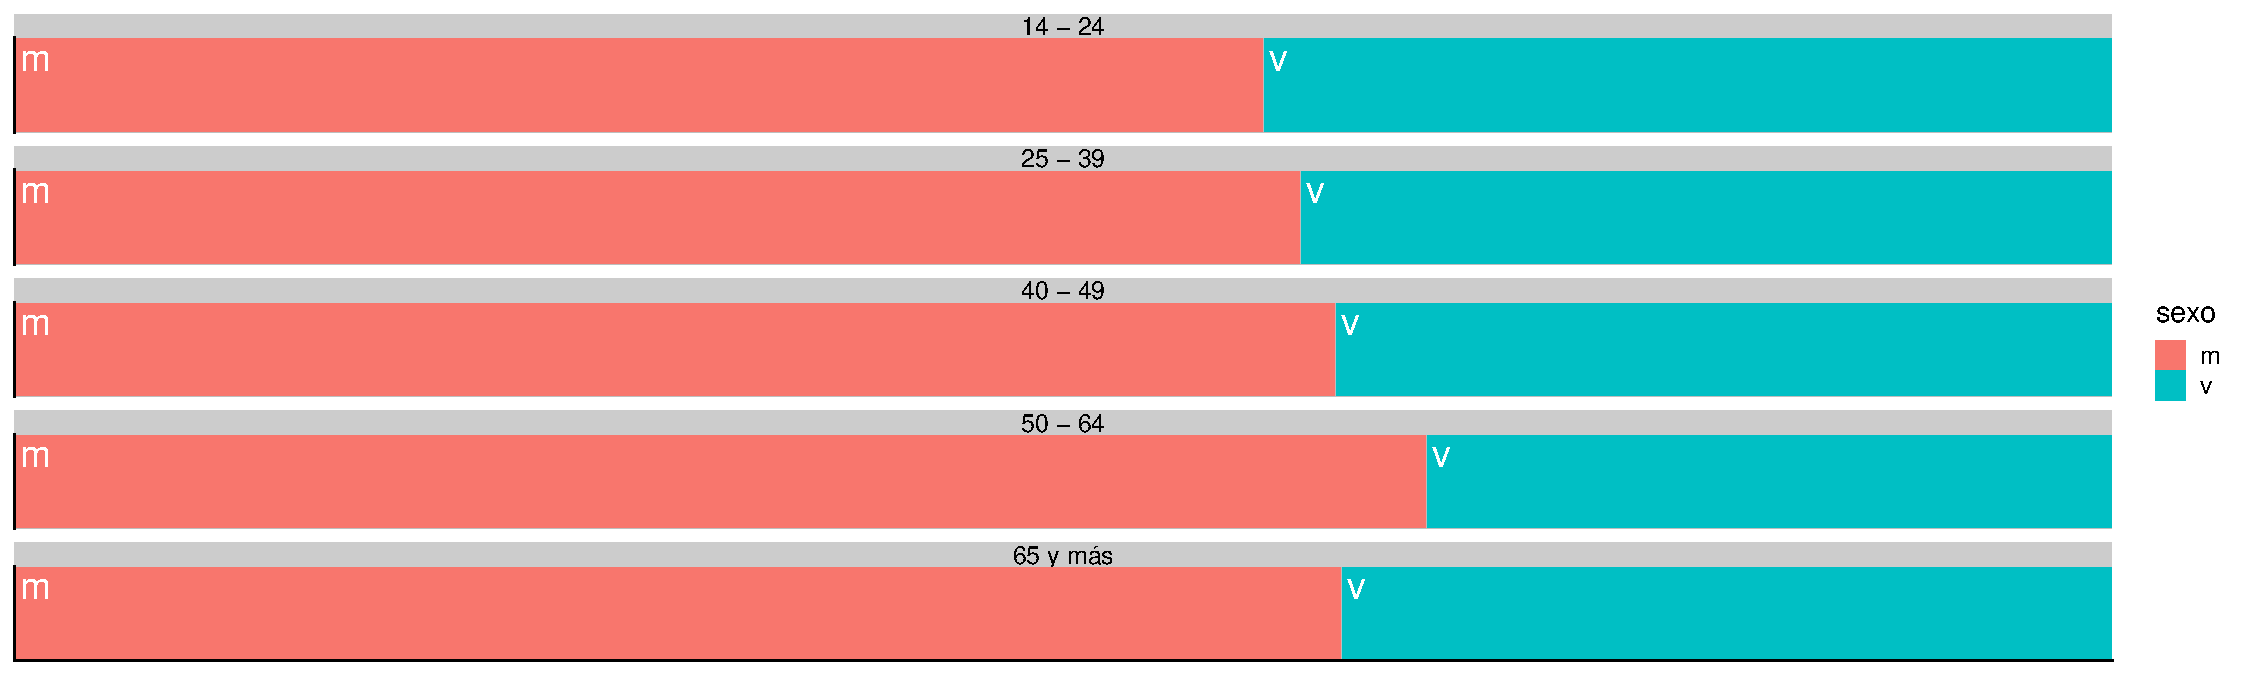
\includegraphics{bookdown_files/figure-latex/unnamed-chunk-66-1.pdf}

\begin{itemize}
\tightlist
\item
  Ahora que tenemos una idea de lo que queremos gráficar lo podemos poner adentro de una función que grafique.
\end{itemize}

\begin{Shaded}
\begin{Highlighting}[]
\CommentTok{# definimos la función}
\NormalTok{graficar_pais <-}\StringTok{ }\ControlFlowTok{function}\NormalTok{(data, pais)\{}
  
  \KeywordTok{ggplot}\NormalTok{(data, }\KeywordTok{aes}\NormalTok{(year, lifeExp, }\DataTypeTok{size=}\NormalTok{ pop, }\DataTypeTok{color=}\NormalTok{gdpPercap))}\OperatorTok{+}
\StringTok{    }\KeywordTok{geom_point}\NormalTok{()}\OperatorTok{+}
\StringTok{    }\KeywordTok{geom_line}\NormalTok{(}\DataTypeTok{alpha=}\FloatTok{0.6}\NormalTok{)}\OperatorTok{+}
\StringTok{    }\KeywordTok{labs}\NormalTok{(}\DataTypeTok{title =}\NormalTok{ pais)}
\NormalTok{\}}
\end{Highlighting}
\end{Shaded}

probamos la función para un caso

\begin{Shaded}
\begin{Highlighting}[]
\KeywordTok{graficar_pais}\NormalTok{(data_argentina, }\StringTok{'Argentina'}\NormalTok{)}
\end{Highlighting}
\end{Shaded}

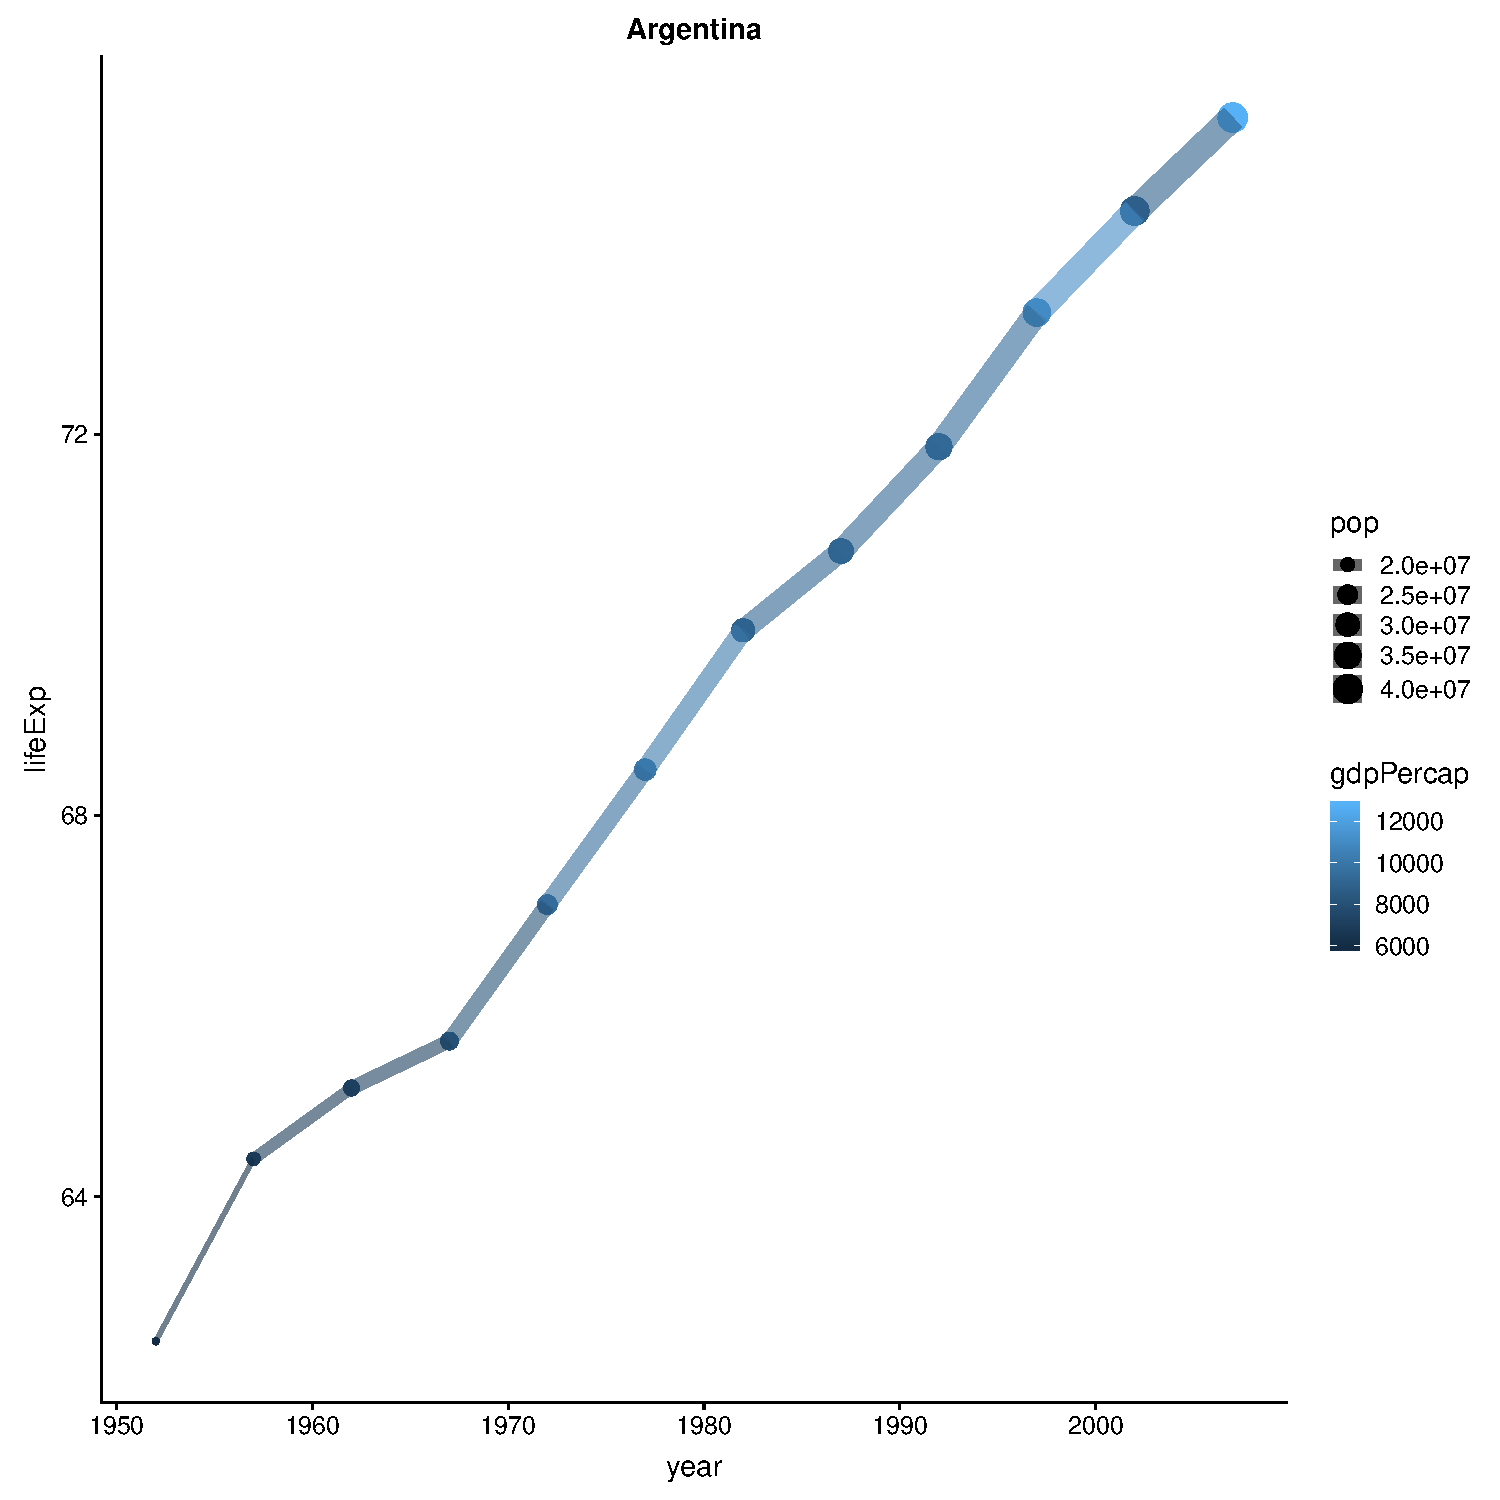
\includegraphics{bookdown_files/figure-latex/unnamed-chunk-68-1.pdf}

\begin{itemize}
\tightlist
\item
  Nos armamos un dataset nesteado
\end{itemize}

\begin{Shaded}
\begin{Highlighting}[]
\NormalTok{gapminder_nest <-}\StringTok{ }\NormalTok{gapminder_unfiltered }\OperatorTok\StringTok{ }
\StringTok{  }\KeywordTok{group_by}\NormalTok{(country) }\OperatorTok\StringTok{ }
\StringTok{  }\KeywordTok{nest}\NormalTok{()}

\NormalTok{gapminder_nest }\OperatorTok\StringTok{ }
\StringTok{  }\KeywordTok{sample_n}\NormalTok{(}\DecValTok{10}\NormalTok{)}
\end{Highlighting}
\end{Shaded}

\begin{verbatim}
## # A tibble: 10 x 2
##    country          data             
##    <fct>            <list>           
##  1 Sweden           <tibble [58 x 5]>
##  2 Mali             <tibble [12 x 5]>
##  3 French Polynesia <tibble [9 x 5]> 
##  4 Colombia         <tibble [12 x 5]>
##  5 Norway           <tibble [58 x 5]>
##  6 Belgium          <tibble [57 x 5]>
##  7 Armenia          <tibble [4 x 5]> 
##  8 Djibouti         <tibble [12 x 5]>
##  9 Brazil           <tibble [12 x 5]>
## 10 Canada           <tibble [57 x 5]>
\end{verbatim}

\begin{itemize}
\tightlist
\item
  Ahora podemos crear una nueva columna que contenga los gráficos
\end{itemize}

\begin{Shaded}
\begin{Highlighting}[]
\NormalTok{gapminder_nest <-}\StringTok{ }\NormalTok{gapminder_nest }\OperatorTok\StringTok{ }
\StringTok{  }\KeywordTok{mutate}\NormalTok{(}\DataTypeTok{grafico=} \KeywordTok{map2}\NormalTok{(}\DataTypeTok{.x =}\NormalTok{ data, }\DataTypeTok{.y =}\NormalTok{ country,}\DataTypeTok{.f =}\NormalTok{  graficar_pais))}

\NormalTok{gapminder_nest }\OperatorTok\StringTok{ }
\StringTok{  }\KeywordTok{sample_n}\NormalTok{(}\DecValTok{10}\NormalTok{)}
\end{Highlighting}
\end{Shaded}

\begin{verbatim}
## # A tibble: 10 x 3
##    country                data              grafico
##    <fct>                  <list>            <list> 
##  1 Tajikistan             <tibble [4 x 5]>  <gg>   
##  2 Brunei                 <tibble [8 x 5]>  <gg>   
##  3 Kazakhstan             <tibble [4 x 5]>  <gg>   
##  4 Guadeloupe             <tibble [1 x 5]>  <gg>   
##  5 Singapore              <tibble [12 x 5]> <gg>   
##  6 Libya                  <tibble [13 x 5]> <gg>   
##  7 Bosnia and Herzegovina <tibble [12 x 5]> <gg>   
##  8 Chad                   <tibble [12 x 5]> <gg>   
##  9 Moldova                <tibble [5 x 5]>  <gg>   
## 10 Jamaica                <tibble [12 x 5]> <gg>
\end{verbatim}

Veamos un ejemplo

\begin{Shaded}
\begin{Highlighting}[]
\NormalTok{gapminder_nest}\OperatorTok{$}\NormalTok{grafico[}\DecValTok{2}\NormalTok{]}
\end{Highlighting}
\end{Shaded}

\begin{verbatim}
## [[1]]
\end{verbatim}

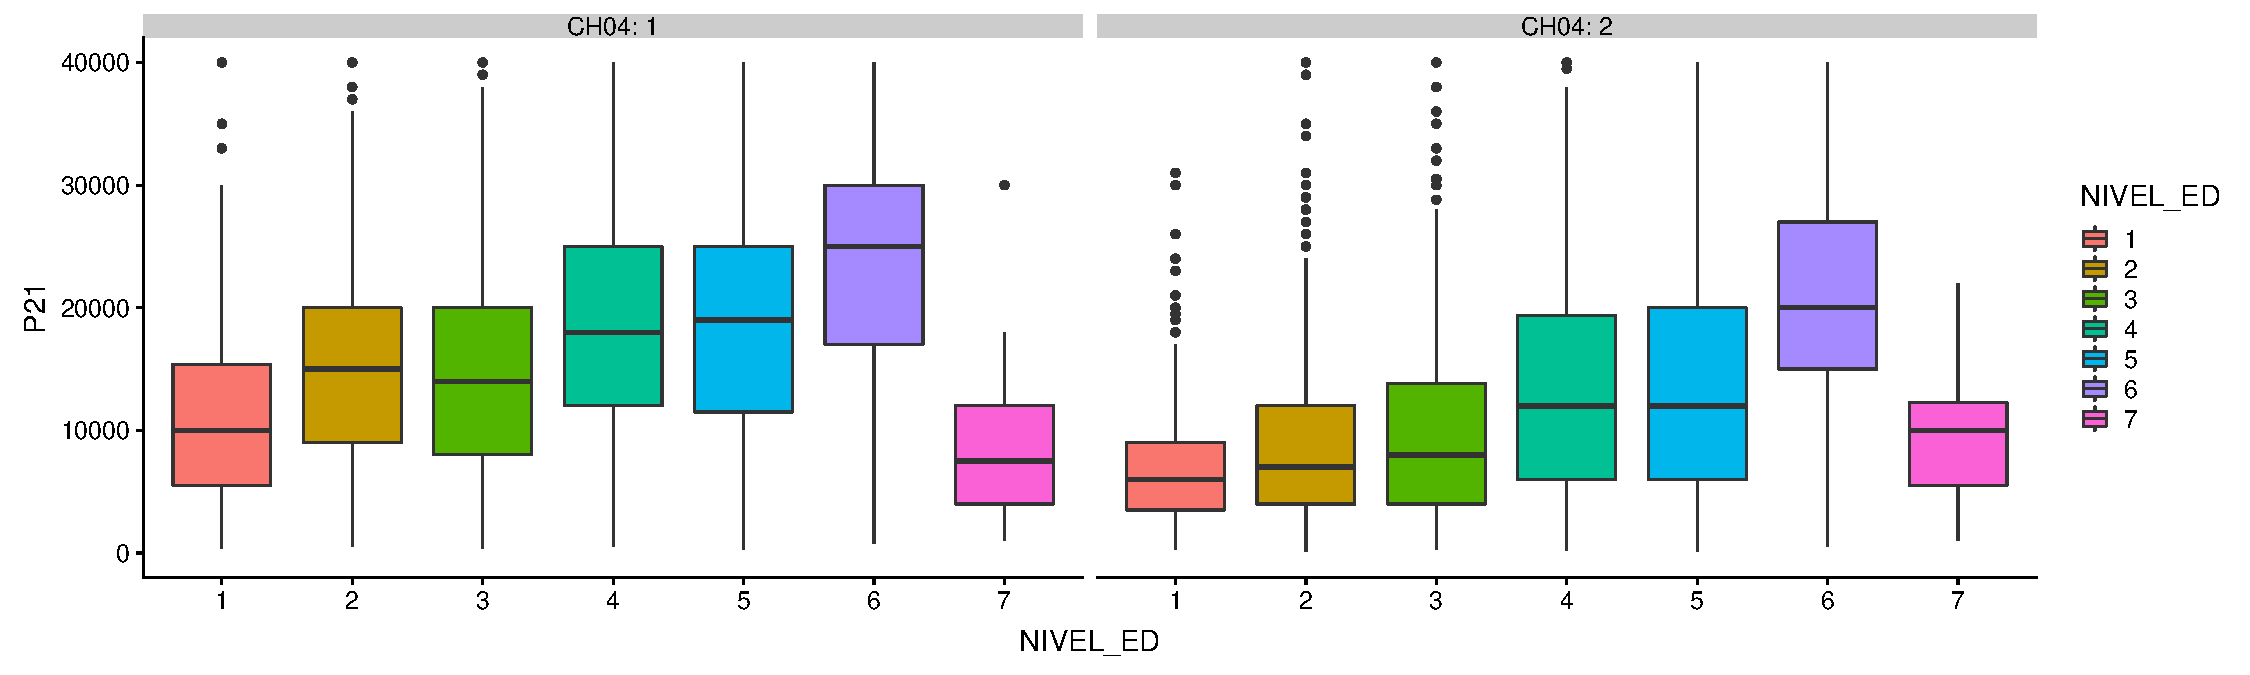
\includegraphics{bookdown_files/figure-latex/unnamed-chunk-71-1.pdf}

Ahora podemos guardar todos los gráficos en un archivo PDF

\begin{Shaded}
\begin{Highlighting}[]
\KeywordTok{pdf}\NormalTok{(}\StringTok{'resultados/graficos_gapminder.pdf'}\NormalTok{)}
\NormalTok{gapminder_nest}\OperatorTok{$}\NormalTok{grafico}
\KeywordTok{dev.off}\NormalTok{()}
\end{Highlighting}
\end{Shaded}

\hypertarget{visualizacion-de-la-informacion}{%
\chapter{Visualización de la información}\label{visualizacion-de-la-informacion}}

En esta clase veremos como realizar gráficos en R, tanto los comandos básicos como utilizando la librería GGPLOT.

\begin{itemize}
\tightlist
\item
  Gráficos básicos de R (función ``plot''): Comandos para la visualización ágil de la información
\item
  Gráficos elaborados en R (función ``ggplot''):
\item
  Gráficos de línea, barras, Boxplots y distribuciones de densidad
\item
  Parámetros de los gráficos: Leyendas, ejes, títulos, notas, colores
\item
  Gráficos con múltiples cruces de variables.
\end{itemize}

\hypertarget{explicacion-2}{%
\section{Explicación}\label{explicacion-2}}

\hypertarget{graficos-basicos-en-r}{%
\subsection{Gráficos Básicos en R}\label{graficos-basicos-en-r}}

Rbase tiene algunos comandos genéricos para realizar gráficos, que se adaptan al tipo de información que se le pide graficar, por ejemplo:

\begin{itemize}
\tightlist
\item
  plot()
\item
  hist()
\end{itemize}

\begin{Shaded}
\begin{Highlighting}[]
\CommentTok{# iris es un set de datos clásico, que ya viene incorporado en R}
\NormalTok{iris[}\DecValTok{10}\NormalTok{,]}
\end{Highlighting}
\end{Shaded}

\begin{verbatim}
##    Sepal.Length Sepal.Width Petal.Length Petal.Width Species
## 10          4.9         3.1          1.5         0.1  setosa
\end{verbatim}

\begin{Shaded}
\begin{Highlighting}[]
\KeywordTok{plot}\NormalTok{(iris)}
\end{Highlighting}
\end{Shaded}

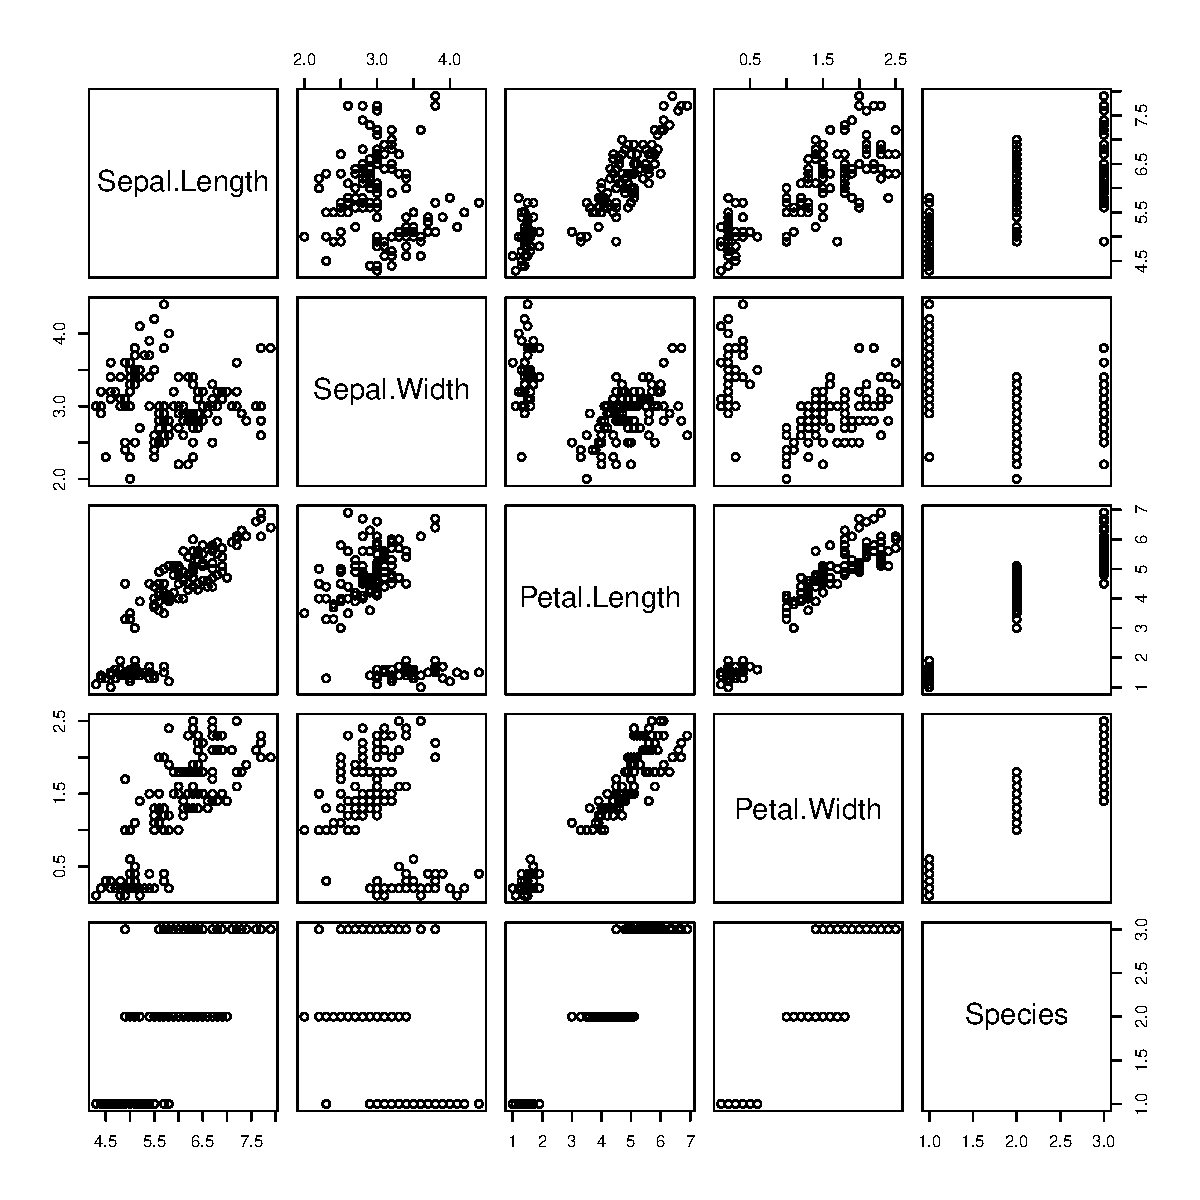
\includegraphics{bookdown_files/figure-latex/unnamed-chunk-73-1.pdf}

\begin{Shaded}
\begin{Highlighting}[]
\CommentTok{#Al especificar una variable, puedo ver el valor que toma cada uno de sus registros (Index)}
\KeywordTok{plot}\NormalTok{(iris}\OperatorTok{$}\NormalTok{Sepal.Length,}\DataTypeTok{type =} \StringTok{"p"}\NormalTok{) }\CommentTok{# Un punto por cada valor}
\end{Highlighting}
\end{Shaded}

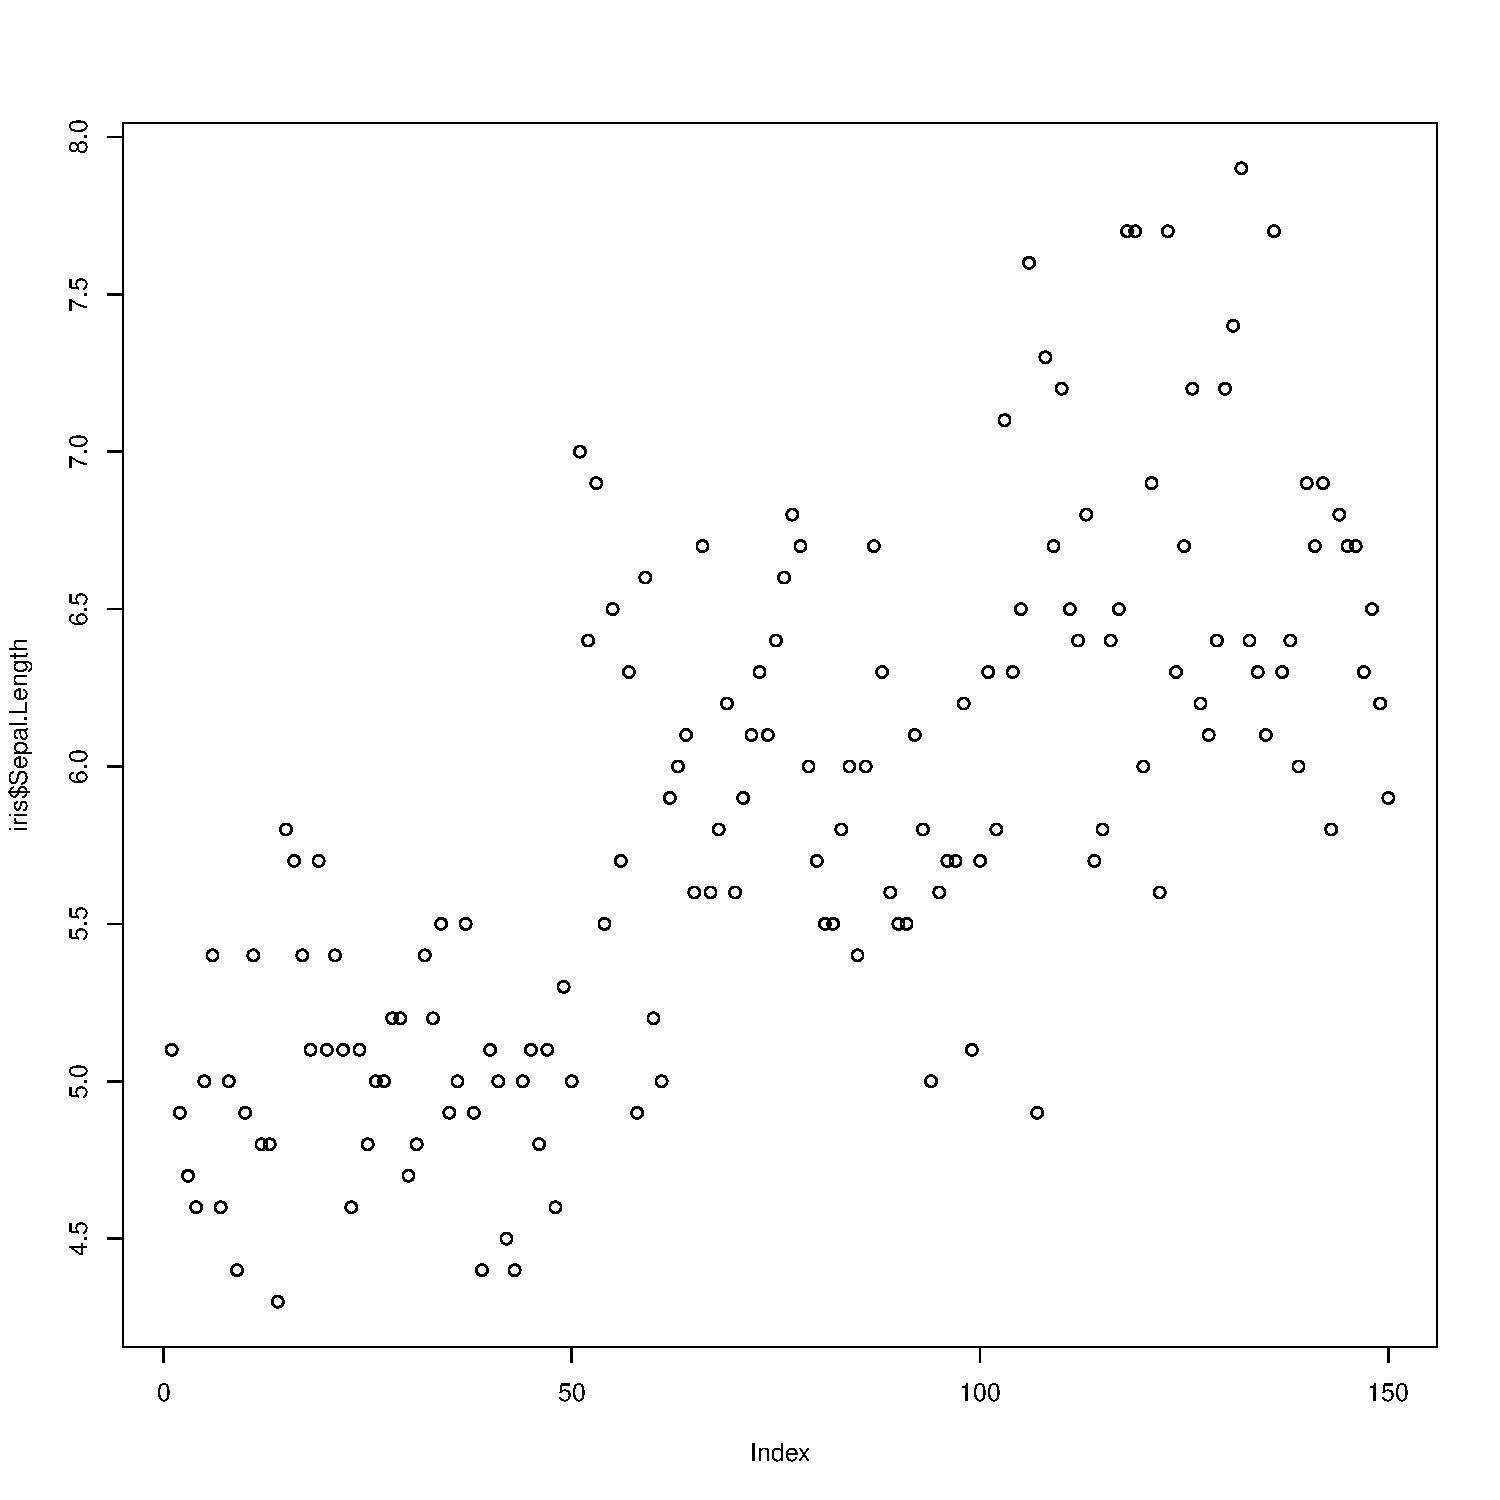
\includegraphics{bookdown_files/figure-latex/unnamed-chunk-74-1.pdf}

\begin{Shaded}
\begin{Highlighting}[]
\KeywordTok{plot}\NormalTok{(iris}\OperatorTok{$}\NormalTok{Sepal.Length,}\DataTypeTok{type =} \StringTok{"l"}\NormalTok{) }\CommentTok{# Una linea que una cada valor}
\end{Highlighting}
\end{Shaded}

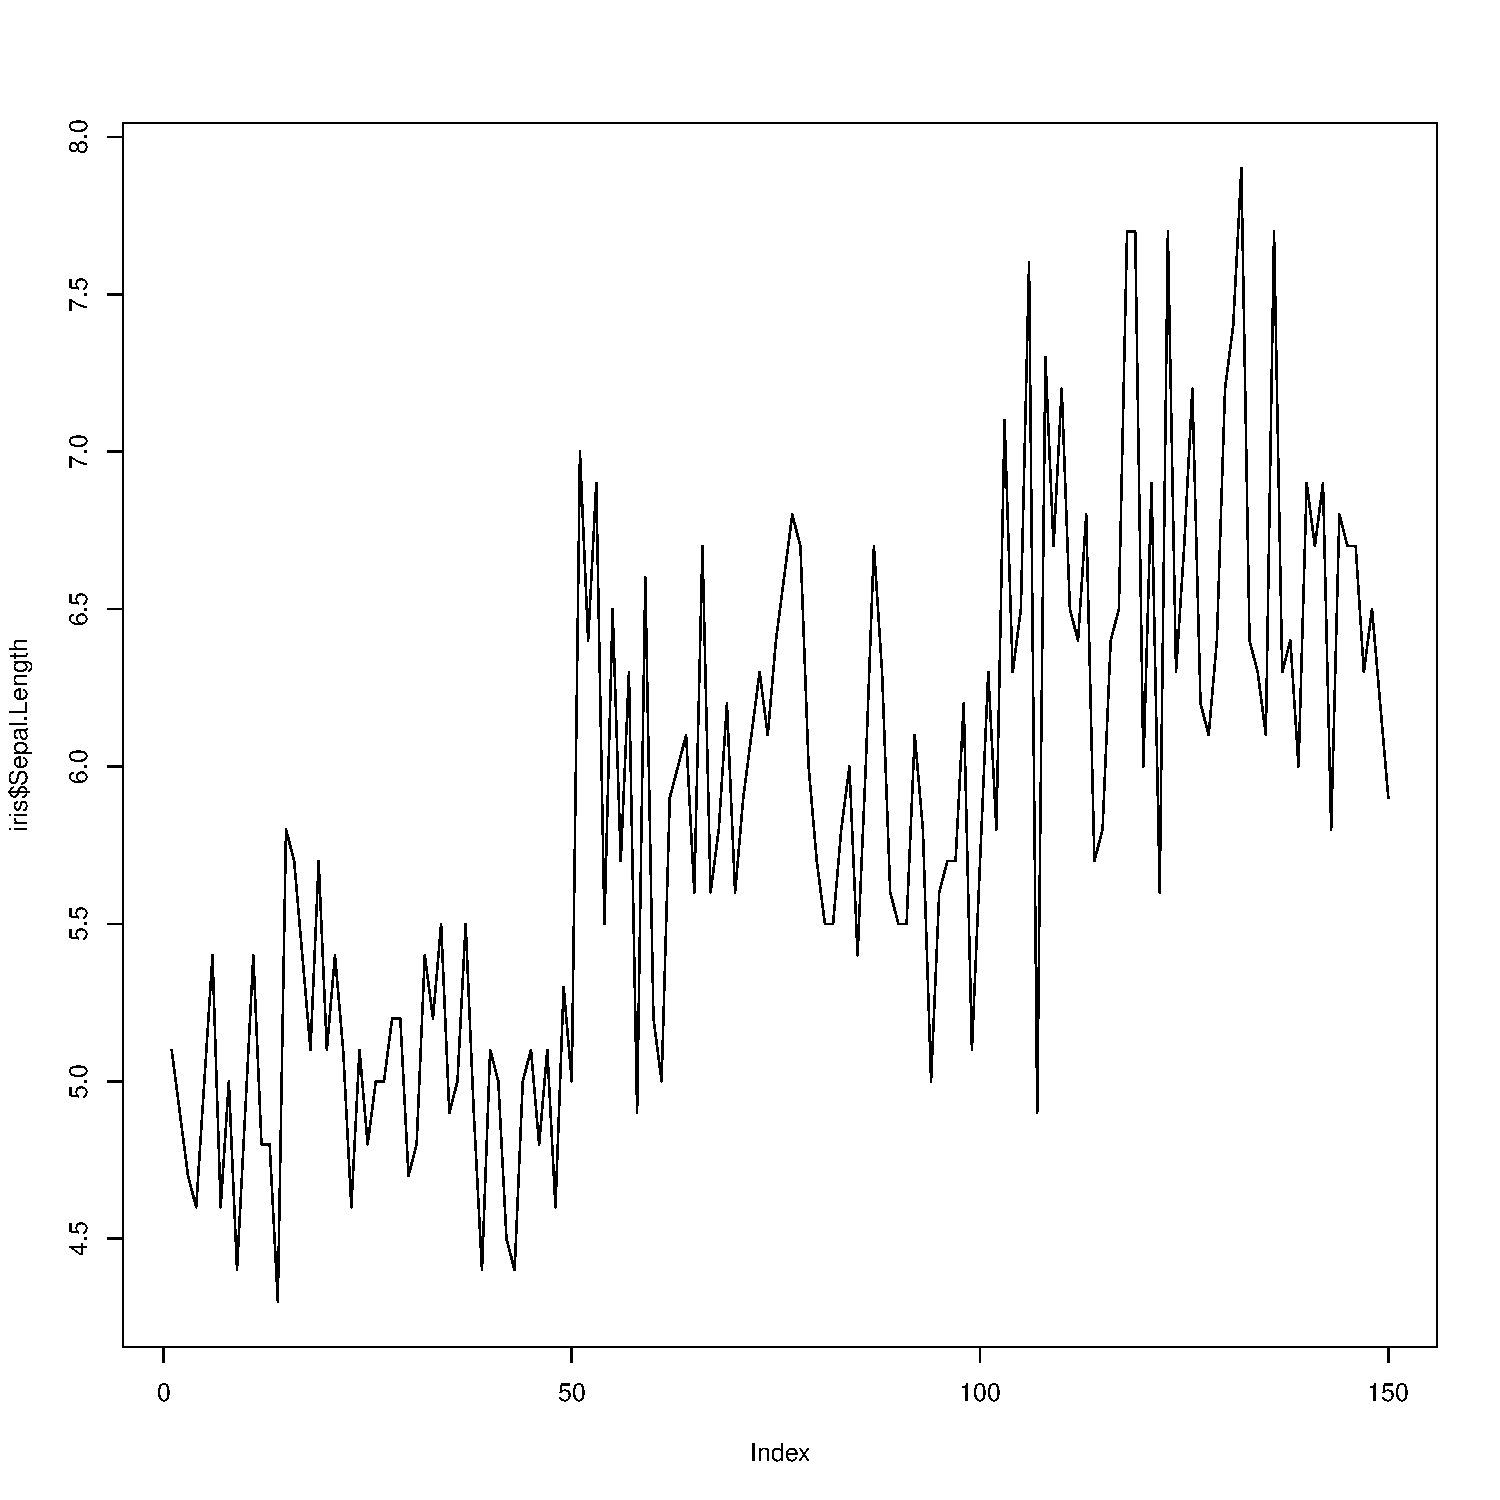
\includegraphics{bookdown_files/figure-latex/unnamed-chunk-74-2.pdf}

\begin{Shaded}
\begin{Highlighting}[]
\KeywordTok{plot}\NormalTok{(iris}\OperatorTok{$}\NormalTok{Sepal.Length,}\DataTypeTok{type =} \StringTok{"b"}\NormalTok{) }\CommentTok{#Ambas}
\end{Highlighting}
\end{Shaded}

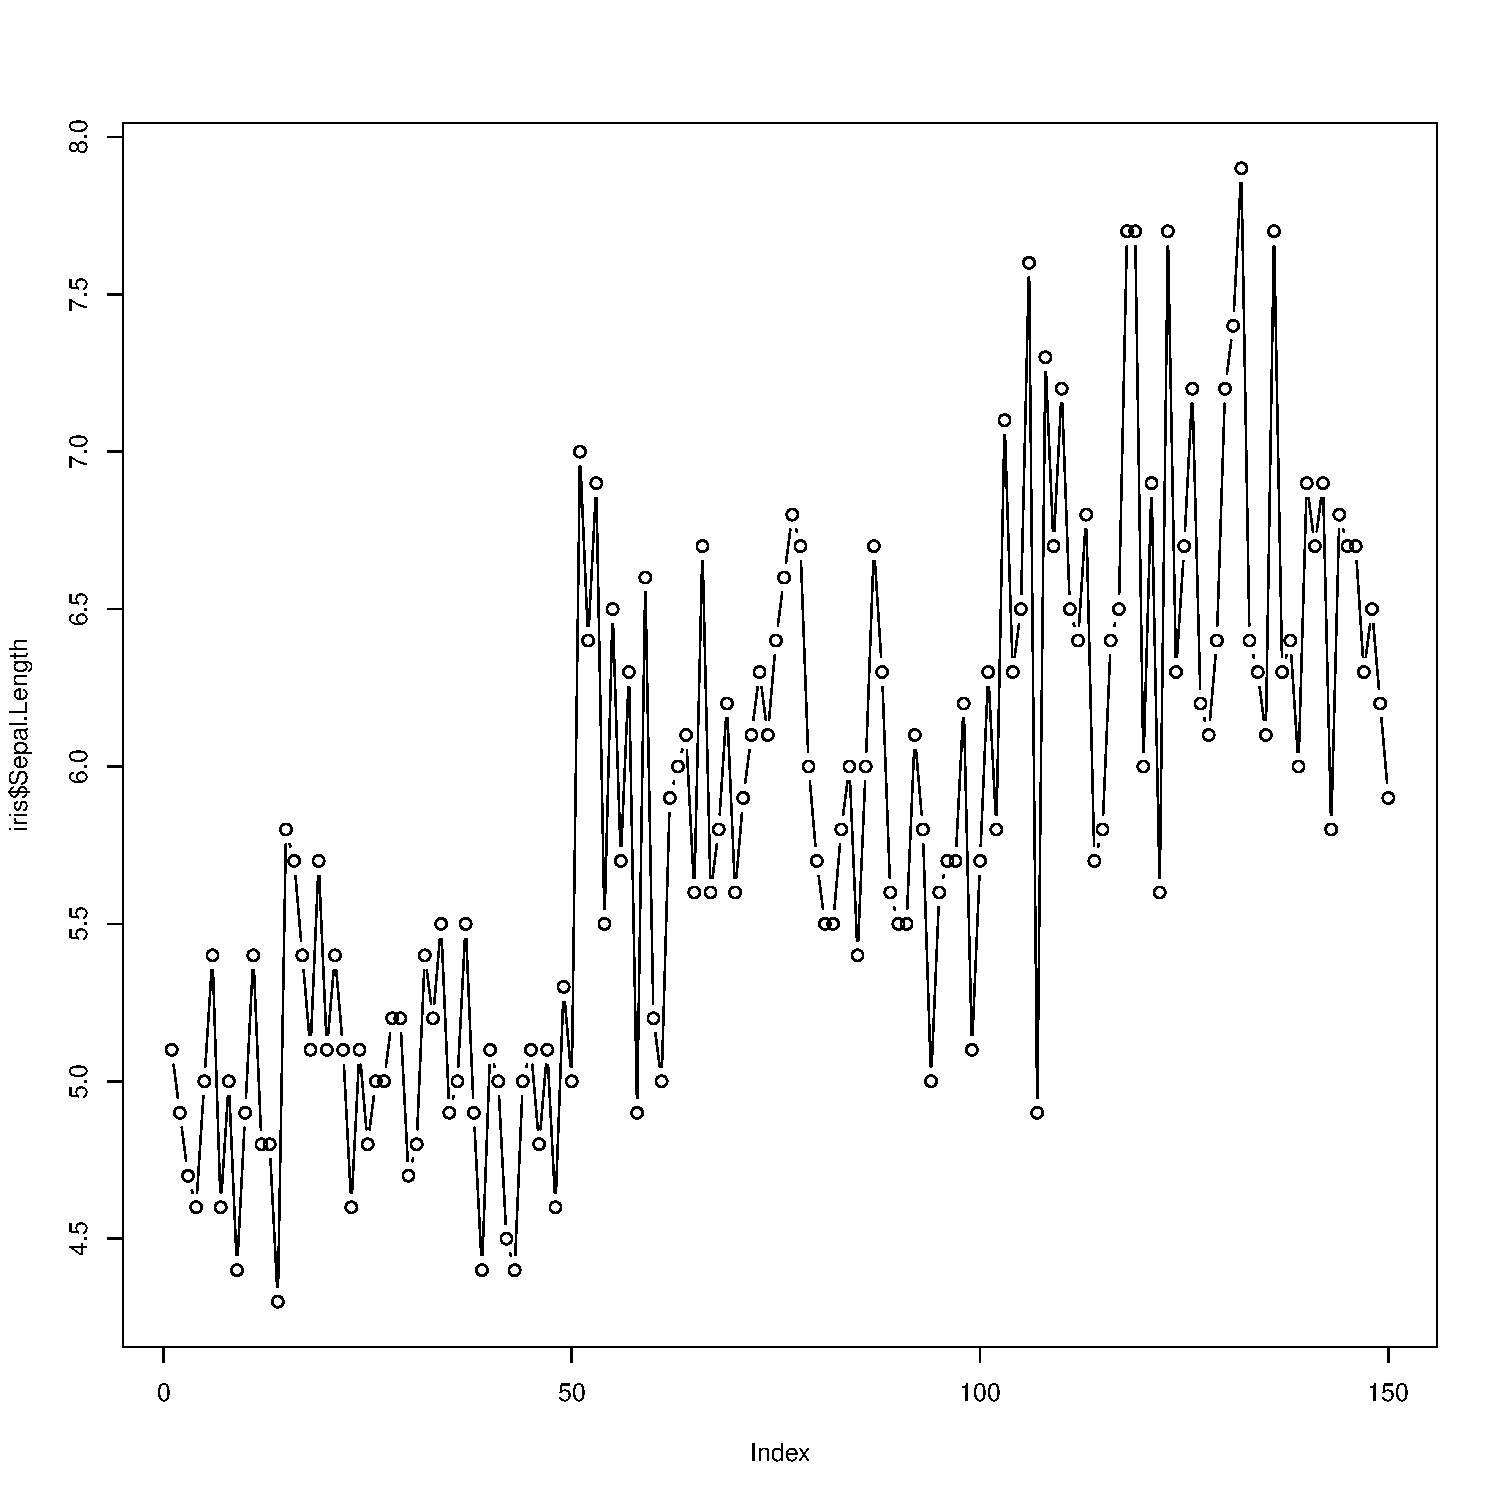
\includegraphics{bookdown_files/figure-latex/unnamed-chunk-74-3.pdf}

\begin{Shaded}
\begin{Highlighting}[]
\KeywordTok{hist}\NormalTok{(iris}\OperatorTok{$}\NormalTok{Sepal.Length, }\DataTypeTok{col =} \StringTok{"lightsalmon1"}\NormalTok{, }\DataTypeTok{main =} \StringTok{"Histograma"}\NormalTok{)}
\end{Highlighting}
\end{Shaded}

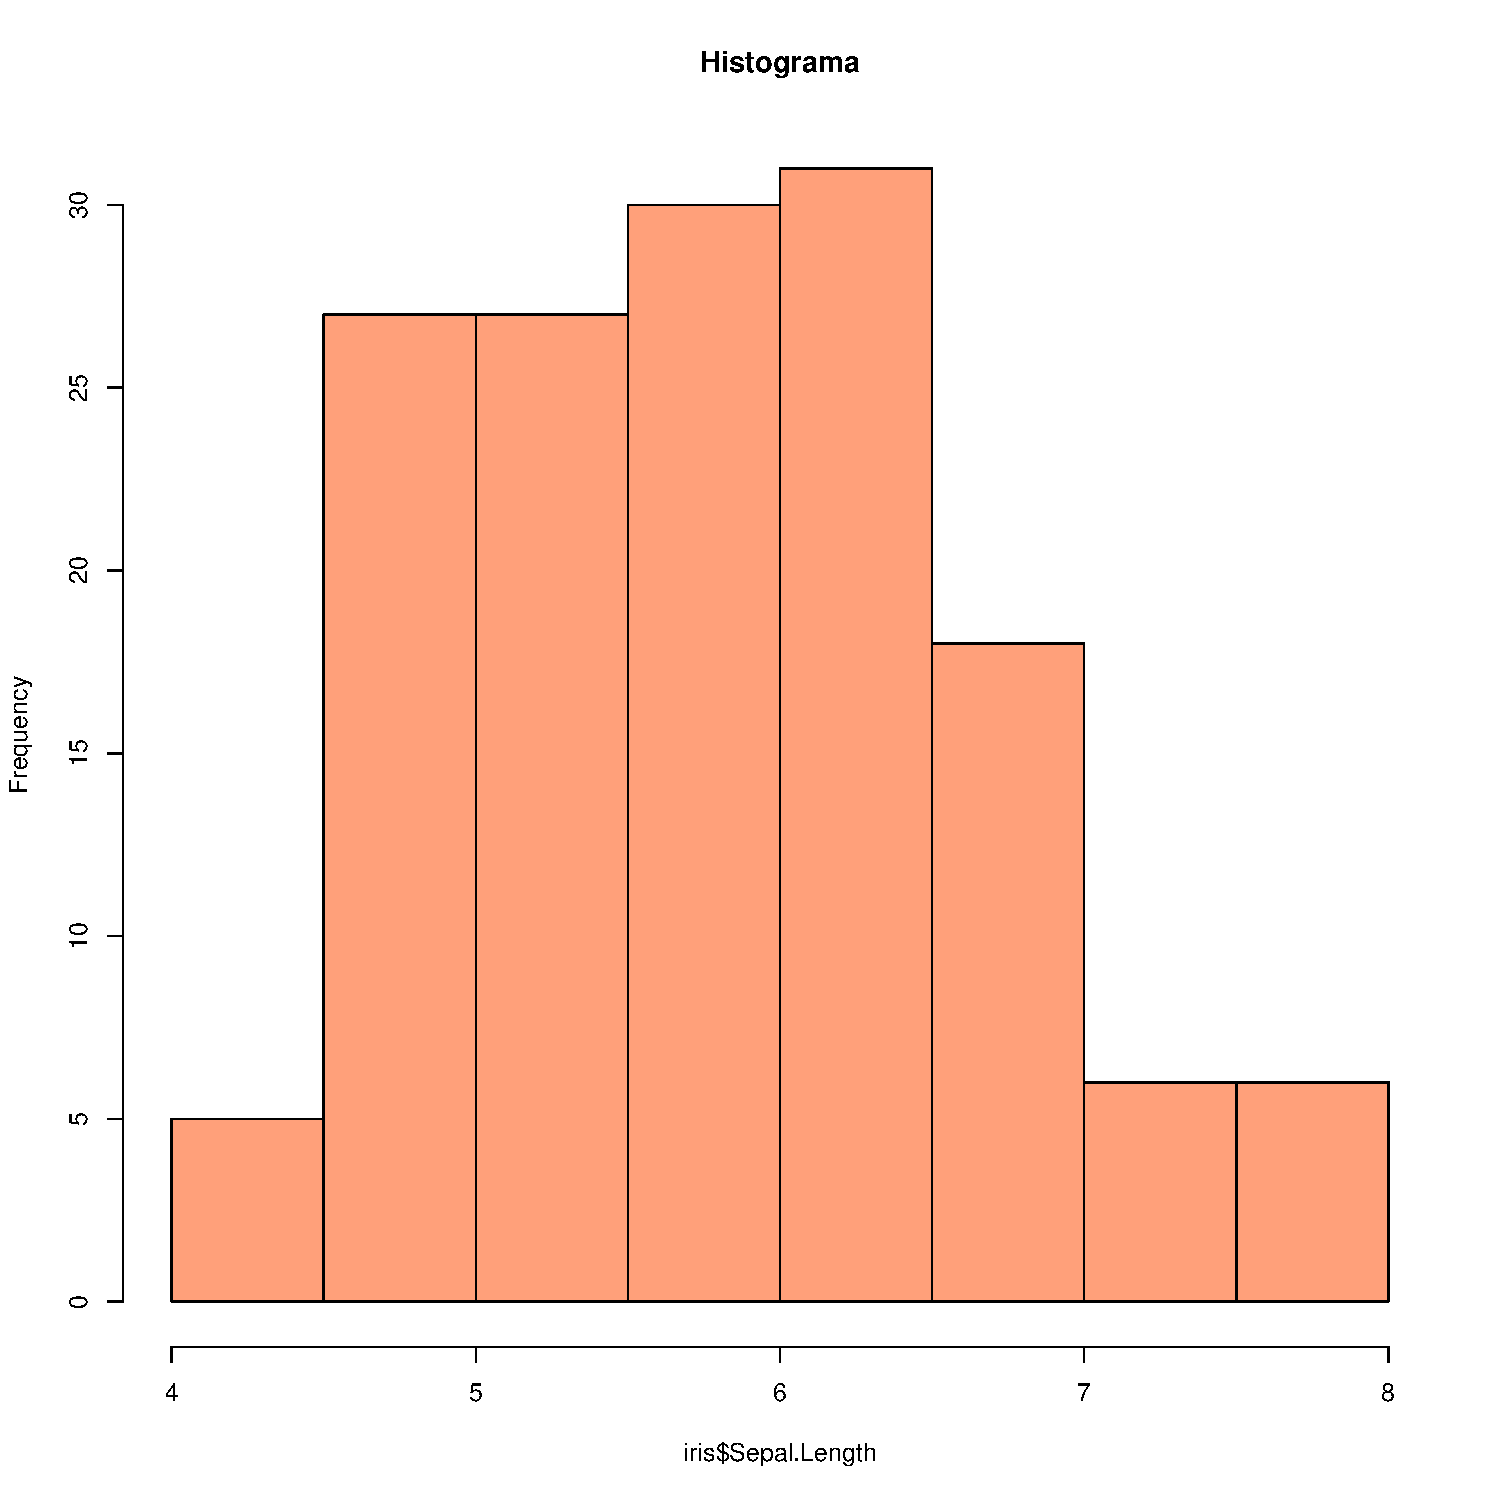
\includegraphics{bookdown_files/figure-latex/unnamed-chunk-74-4.pdf}

\hypertarget{png}{%
\subsubsection{png}\label{png}}

La función \texttt{png()} nos permite grabar una imagen en el disco. Lleva como argumento principal la ruta completa a donde se desea guardar la misma, incluyendo el nombre que queremos dar al archivo. A su vez pueden especificarse otros argumentos como el ancho y largo de la imagen, entre otros.

\begin{Shaded}
\begin{Highlighting}[]
\NormalTok{ruta_archivo <-}\StringTok{ "resultados/grafico1.PNG"}
\NormalTok{ruta_archivo}
\end{Highlighting}
\end{Shaded}

\begin{verbatim}
## [1] "resultados/grafico1.PNG"
\end{verbatim}

\begin{Shaded}
\begin{Highlighting}[]
\KeywordTok{png}\NormalTok{(ruta_archivo)}
\KeywordTok{plot}\NormalTok{(iris}\OperatorTok{$}\NormalTok{Sepal.Length,}\DataTypeTok{type =} \StringTok{"b"}\NormalTok{)}
\KeywordTok{dev.off}\NormalTok{()}
\end{Highlighting}
\end{Shaded}

\begin{verbatim}
## pdf 
##   2
\end{verbatim}

La función \texttt{png()} \emph{abre el dispositivo de imagen} en el directorio especificado. Luego creamos el gráfico que deseamos (o llamamos a uno previamente construido), el cual se desplegará en la ventana inferior derecha de la pantalla de Rstudio. Finalmente con \texttt{dev.off()} se \emph{cierra el dispositivo} y se graban los gráficos.

Los gráficos del R base son útiles para escribir de forma rápida y obtener alguna información mientras trabajamos. Muchos paquetes estadísticos permiten mostrar los resultados de forma gráfica con el comando \texttt{plot} (por ejemplo, las regresiones lineales \texttt{lm()}).

Sin embargo, existen librerías mucho mejores para crear gráficos de nivel de publicación. La más importante es \textbf{ggplot2}, que a su vez tiene extensiones mediante otras librerías.

\hypertarget{ggplot2}{%
\subsection{\texorpdfstring{\href{http://ggplot2.tidyverse.org/reference/}{Ggplot2}}{Ggplot2}}\label{ggplot2}}

\texttt{ggplot} tiene su sintaxis propia. La idea central es pensar los gráficos como una sucesión de capas, que se construyen una a la vez.

\begin{itemize}
\item
  El operador \textbf{\texttt{+}} nos permite incorporar nuevas capas al gráfico.
\item
  El comando \texttt{ggplot()} nos permite definir la fuente de \textbf{datos} y las \textbf{variables} que determinaran los ejes del grafico (x,y), así como el color y la forma de las líneas o puntos,etc.
\item
  Las sucesivas capas nos permiten definir:

  \begin{itemize}
  \tightlist
  \item
    Uno o más tipos de gráficos (de columnas, \texttt{geom\_col()}, de línea, \texttt{geom\_line()}, de puntos, \texttt{geom\_point()}, boxplot, \texttt{geom\_boxplot()})
  \item
    Títulos \texttt{labs()}
  \item
    Estilo del gráfico \texttt{theme()}
  \item
    Escalas de los ejes \texttt{scale\_y\_continuous},\texttt{scale\_x\_discrete}
  \item
    División en subconjuntos \texttt{facet\_wrap()},\texttt{facet\_grid()}
  \end{itemize}
\end{itemize}

\texttt{ggplot} tiene \textbf{muchos} comandos, y no tiene sentido saberlos de memoria, es siempre útil reutilizar gráficos viejos y tener a mano el \href{https://www.rstudio.com/wp-content/uploads/2016/11/ggplot2-cheatsheet-2.1.pdf}{machete}.

\hypertarget{grafico-de-puntos}{%
\subsubsection{Gráfico de Puntos}\label{grafico-de-puntos}}

A continuación se muestra un gráfico de varias capas de construcción, con su correspondiente porción de código. En el mismo se buscará visualizar, a partir de la base de datos \textbf{iris} la relación entre el ancho y el largo de los petalos, mediante un gráfico de puntos.

\begin{Shaded}
\begin{Highlighting}[]
\KeywordTok{library}\NormalTok{(tidyverse) }\CommentTok{# cargamos la librería}
\end{Highlighting}
\end{Shaded}

\begin{Shaded}
\begin{Highlighting}[]
\KeywordTok{ggplot}\NormalTok{(}\DataTypeTok{data =}\NormalTok{ iris, }\KeywordTok{aes}\NormalTok{(}\DataTypeTok{x =}\NormalTok{ Petal.Length, Petal.Width, }\DataTypeTok{color =}\NormalTok{ Species))}\OperatorTok{+}
\StringTok{  }\KeywordTok{geom_point}\NormalTok{(}\DataTypeTok{alpha=}\FloatTok{0.75}\NormalTok{)}\OperatorTok{+}
\StringTok{  }\KeywordTok{labs}\NormalTok{(}\DataTypeTok{title =} \StringTok{"Medidas de los pétalos por especie"}\NormalTok{)}\OperatorTok{+}
\StringTok{  }\KeywordTok{theme}\NormalTok{(}\DataTypeTok{legend.position =} \StringTok{'none'}\NormalTok{)}\OperatorTok{+}
\StringTok{  }\KeywordTok{facet_wrap}\NormalTok{(}\OperatorTok{~}\NormalTok{Species)}
\end{Highlighting}
\end{Shaded}

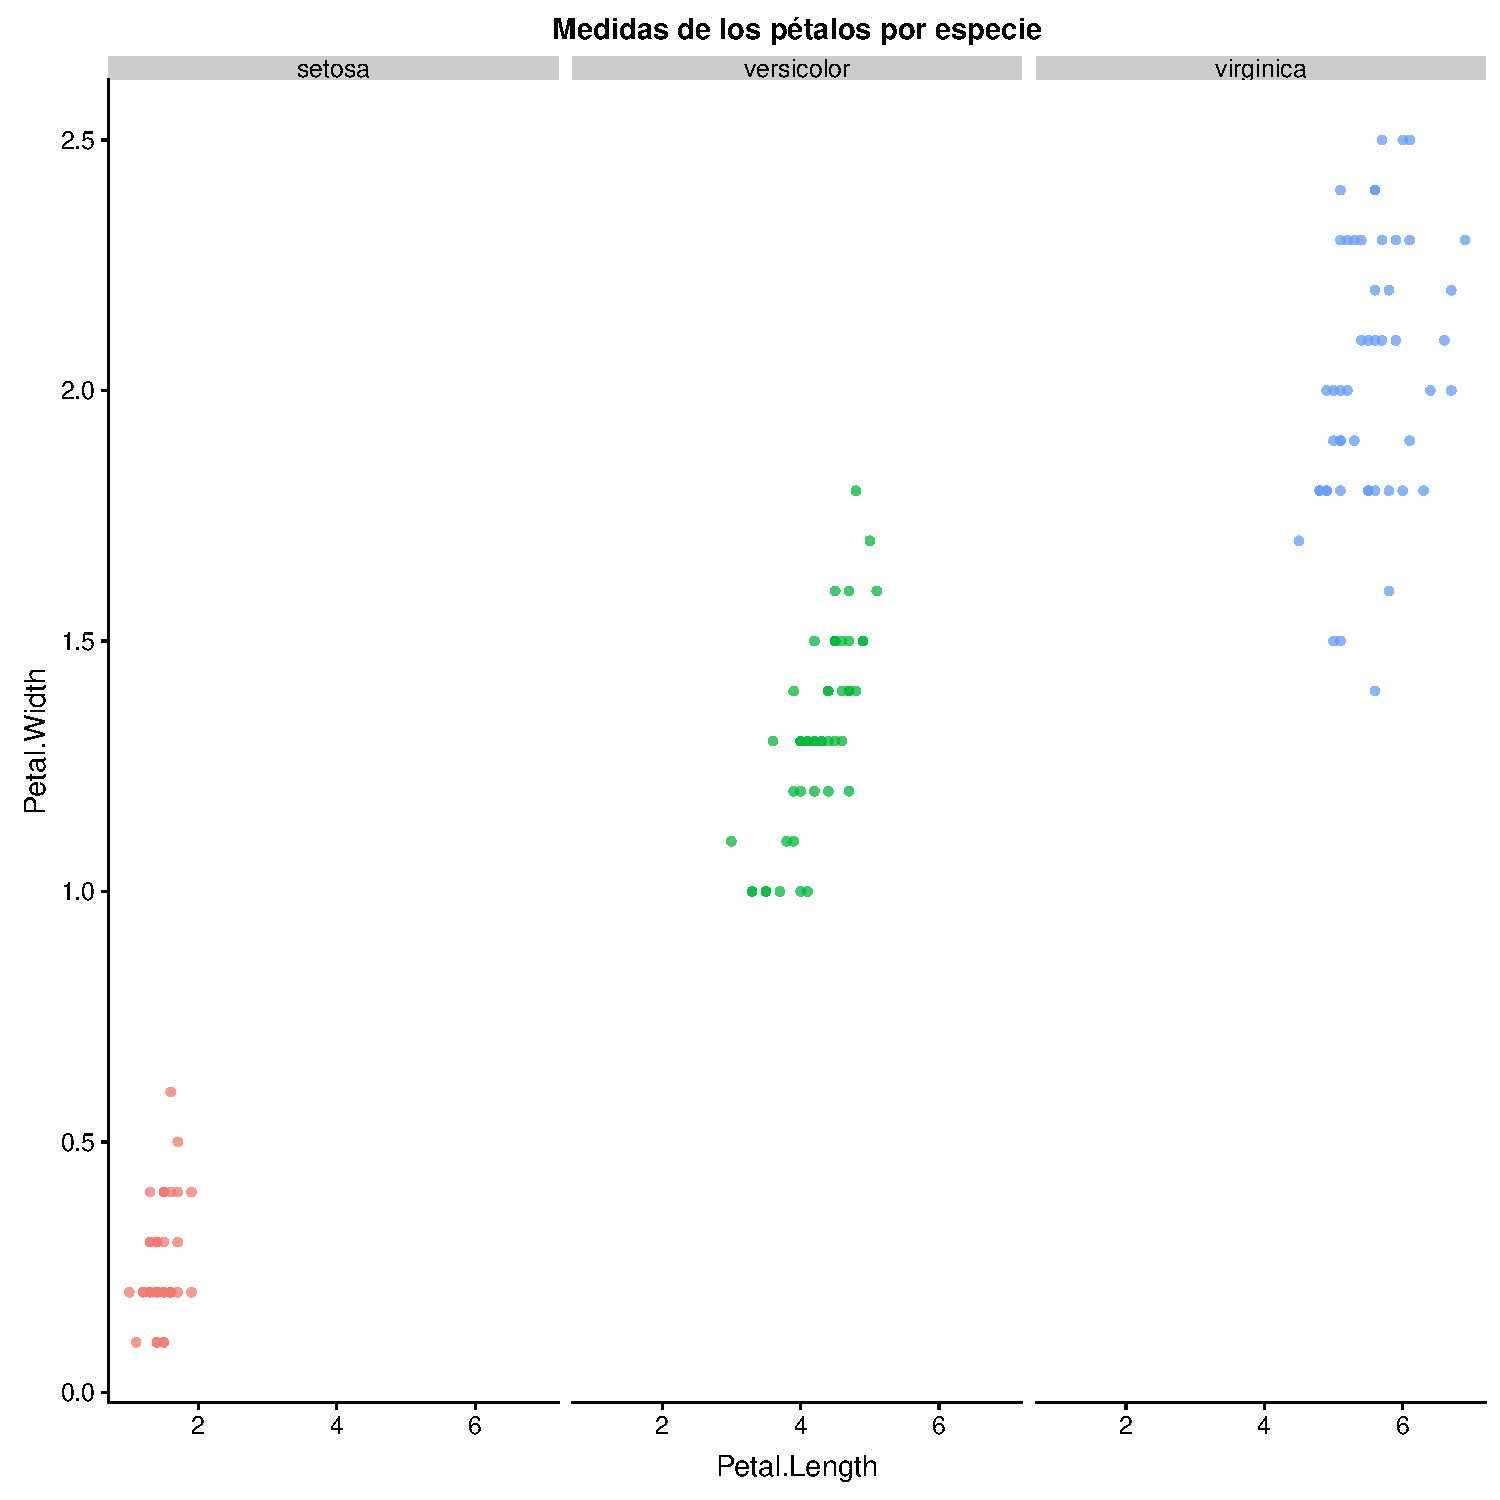
\includegraphics{bookdown_files/figure-latex/unnamed-chunk-77-1.pdf}

\hypertarget{capas-del-grafico}{%
\subsubsection{Capas del Gráfico}\label{capas-del-grafico}}

Veamos ahora, el ``paso a paso'' del armado del mismo.

En primera instancia solo defino los ejes. Y en este caso un color particular para cada Especie.

\begin{Shaded}
\begin{Highlighting}[]
\NormalTok{g <-}\StringTok{ }\KeywordTok{ggplot}\NormalTok{(}\DataTypeTok{data =}\NormalTok{ iris, }\KeywordTok{aes}\NormalTok{(}\DataTypeTok{x =}\NormalTok{ Petal.Length, Petal.Width, }\DataTypeTok{color =}\NormalTok{ Species))}
\NormalTok{g}
\end{Highlighting}
\end{Shaded}

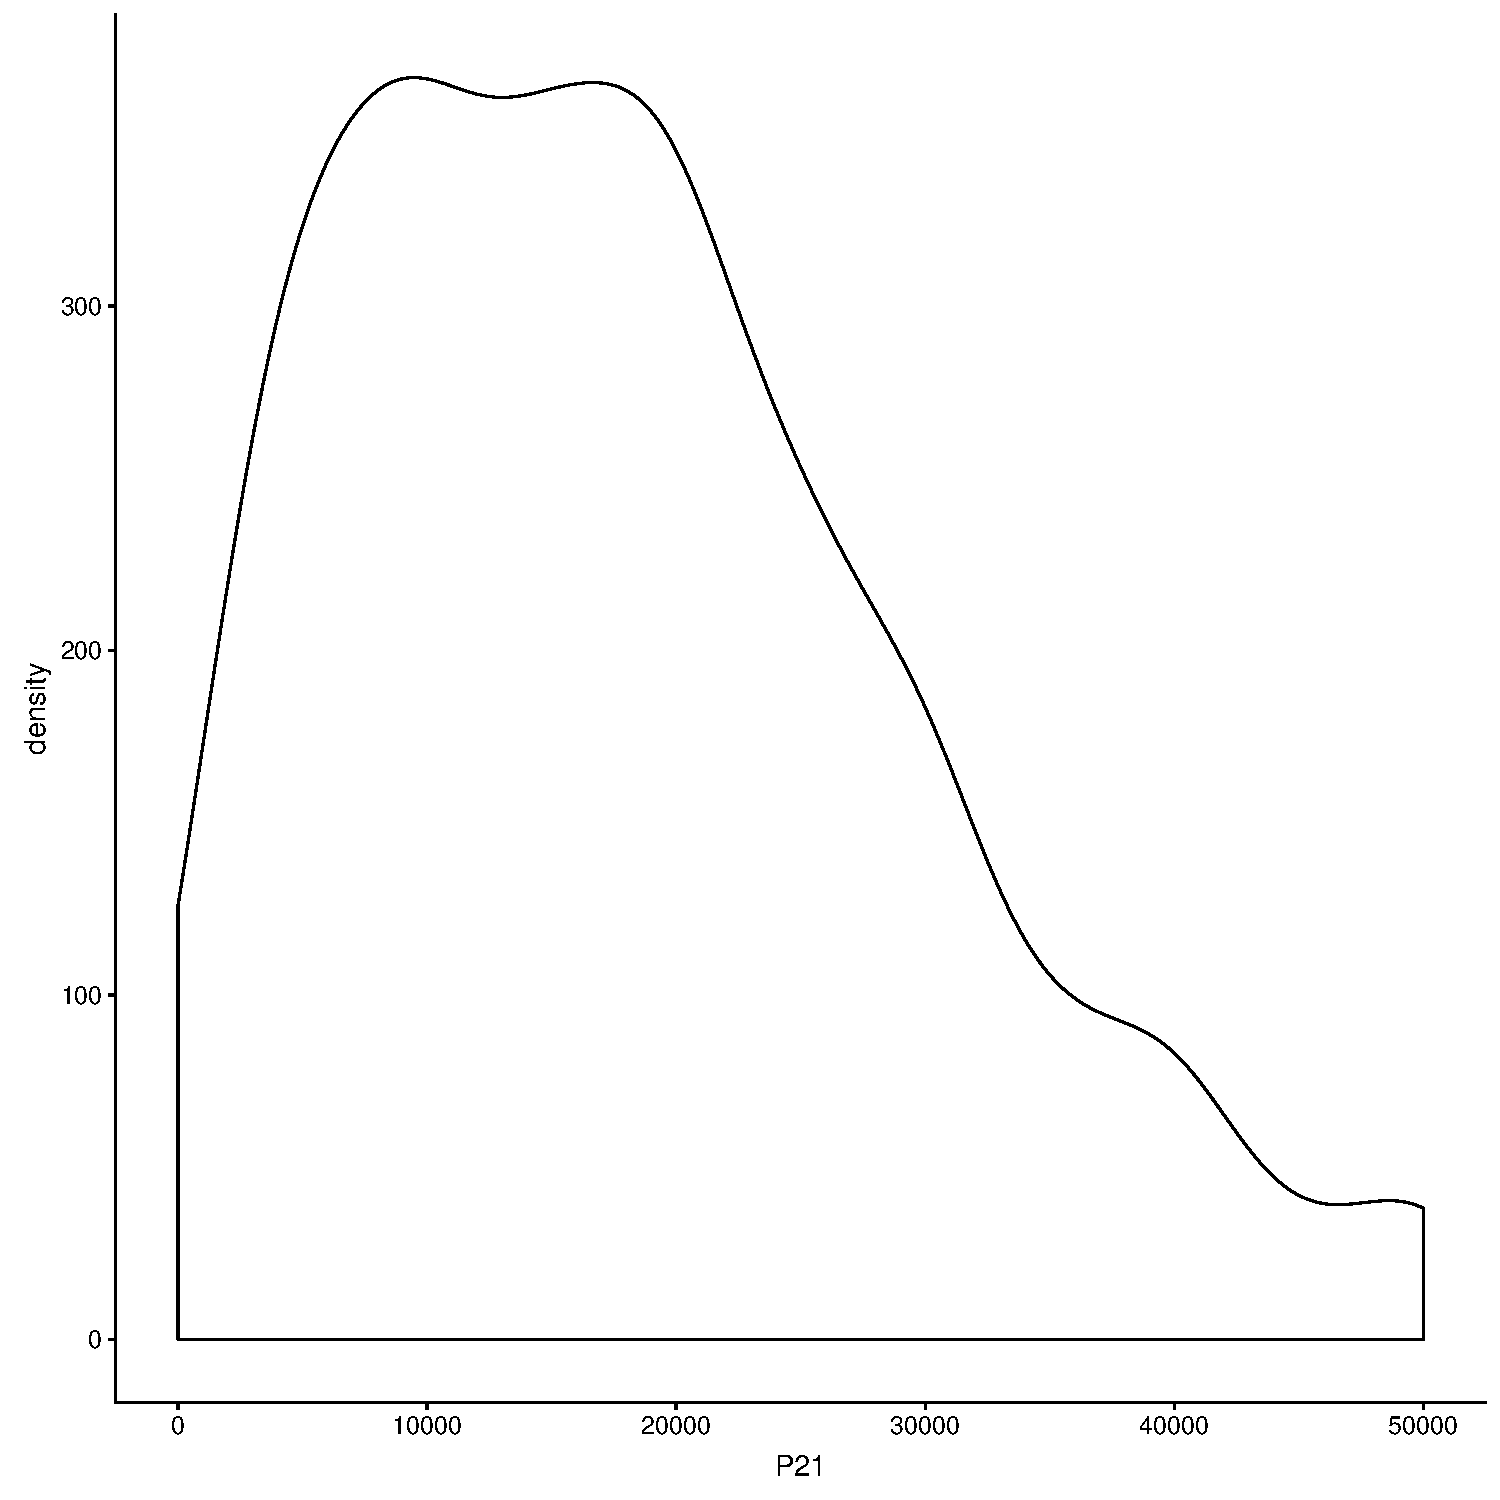
\includegraphics{bookdown_files/figure-latex/unnamed-chunk-78-1.pdf}
Luego, defino el tipo de gráfico. El \emph{alpha} me permite definir la intensidad de los puntos

\begin{Shaded}
\begin{Highlighting}[]
\NormalTok{g <-}\StringTok{ }\NormalTok{g }\OperatorTok{+}\StringTok{  }\KeywordTok{geom_point}\NormalTok{(}\DataTypeTok{alpha=}\FloatTok{0.25}\NormalTok{)}
\NormalTok{g}
\end{Highlighting}
\end{Shaded}

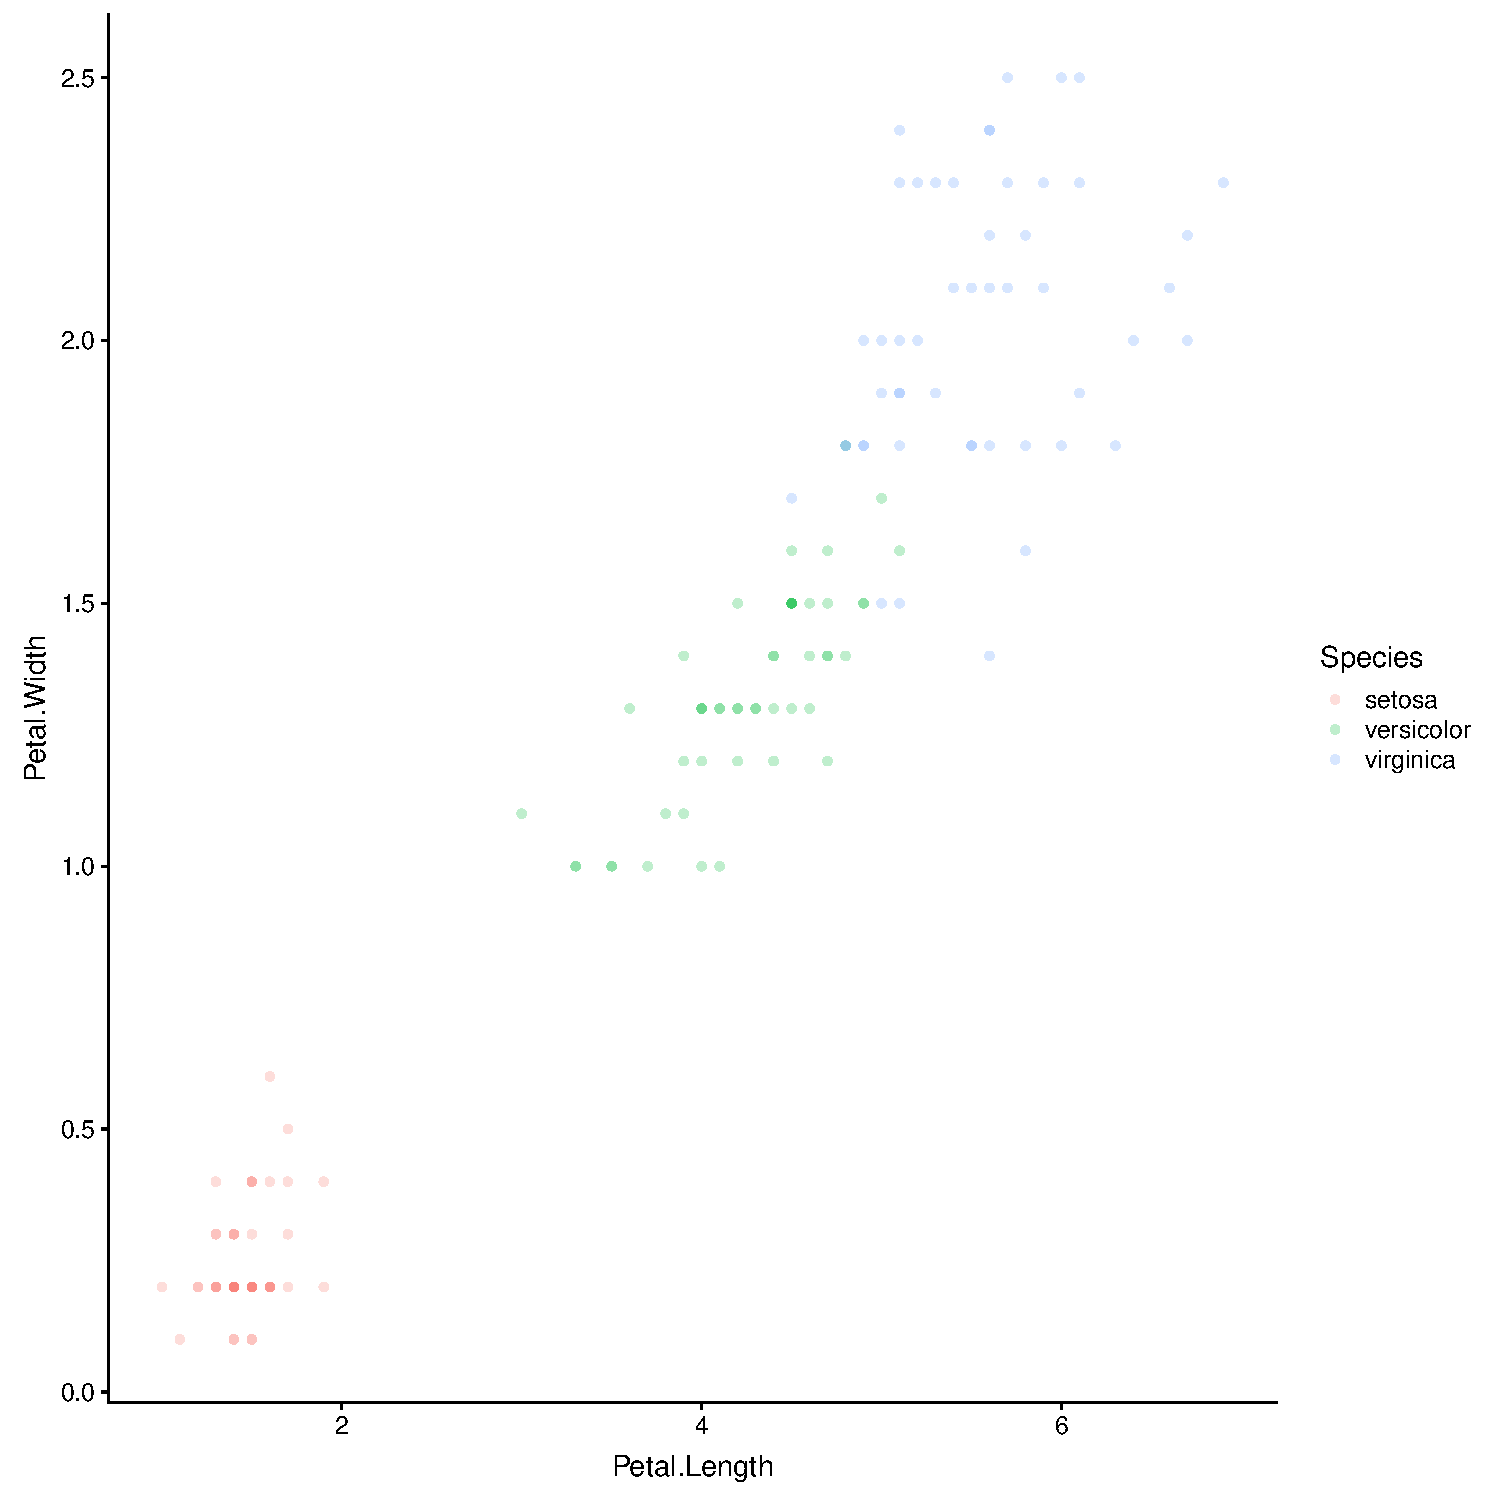
\includegraphics{bookdown_files/figure-latex/unnamed-chunk-79-1.pdf}
Las siguientes tres capas me permiten respectivamente:

\begin{itemize}
\tightlist
\item
  Definir el título del gráfico
\item
  Quitar la leyenda
\item
  Abrir el gráfico en tres fragmentos, uno para cada especie
\end{itemize}

\begin{Shaded}
\begin{Highlighting}[]
\NormalTok{g <-}\StringTok{ }\NormalTok{g }\OperatorTok{+}
\StringTok{  }\KeywordTok{labs}\NormalTok{(}\DataTypeTok{title =} \StringTok{"Medidas de los pétalos por especie"}\NormalTok{)}\OperatorTok{+}
\StringTok{  }\KeywordTok{theme}\NormalTok{(}\DataTypeTok{legend.position =} \StringTok{'none'}\NormalTok{)}\OperatorTok{+}
\StringTok{  }\KeywordTok{facet_wrap}\NormalTok{(}\OperatorTok{~}\NormalTok{Species)}
\NormalTok{g}
\end{Highlighting}
\end{Shaded}

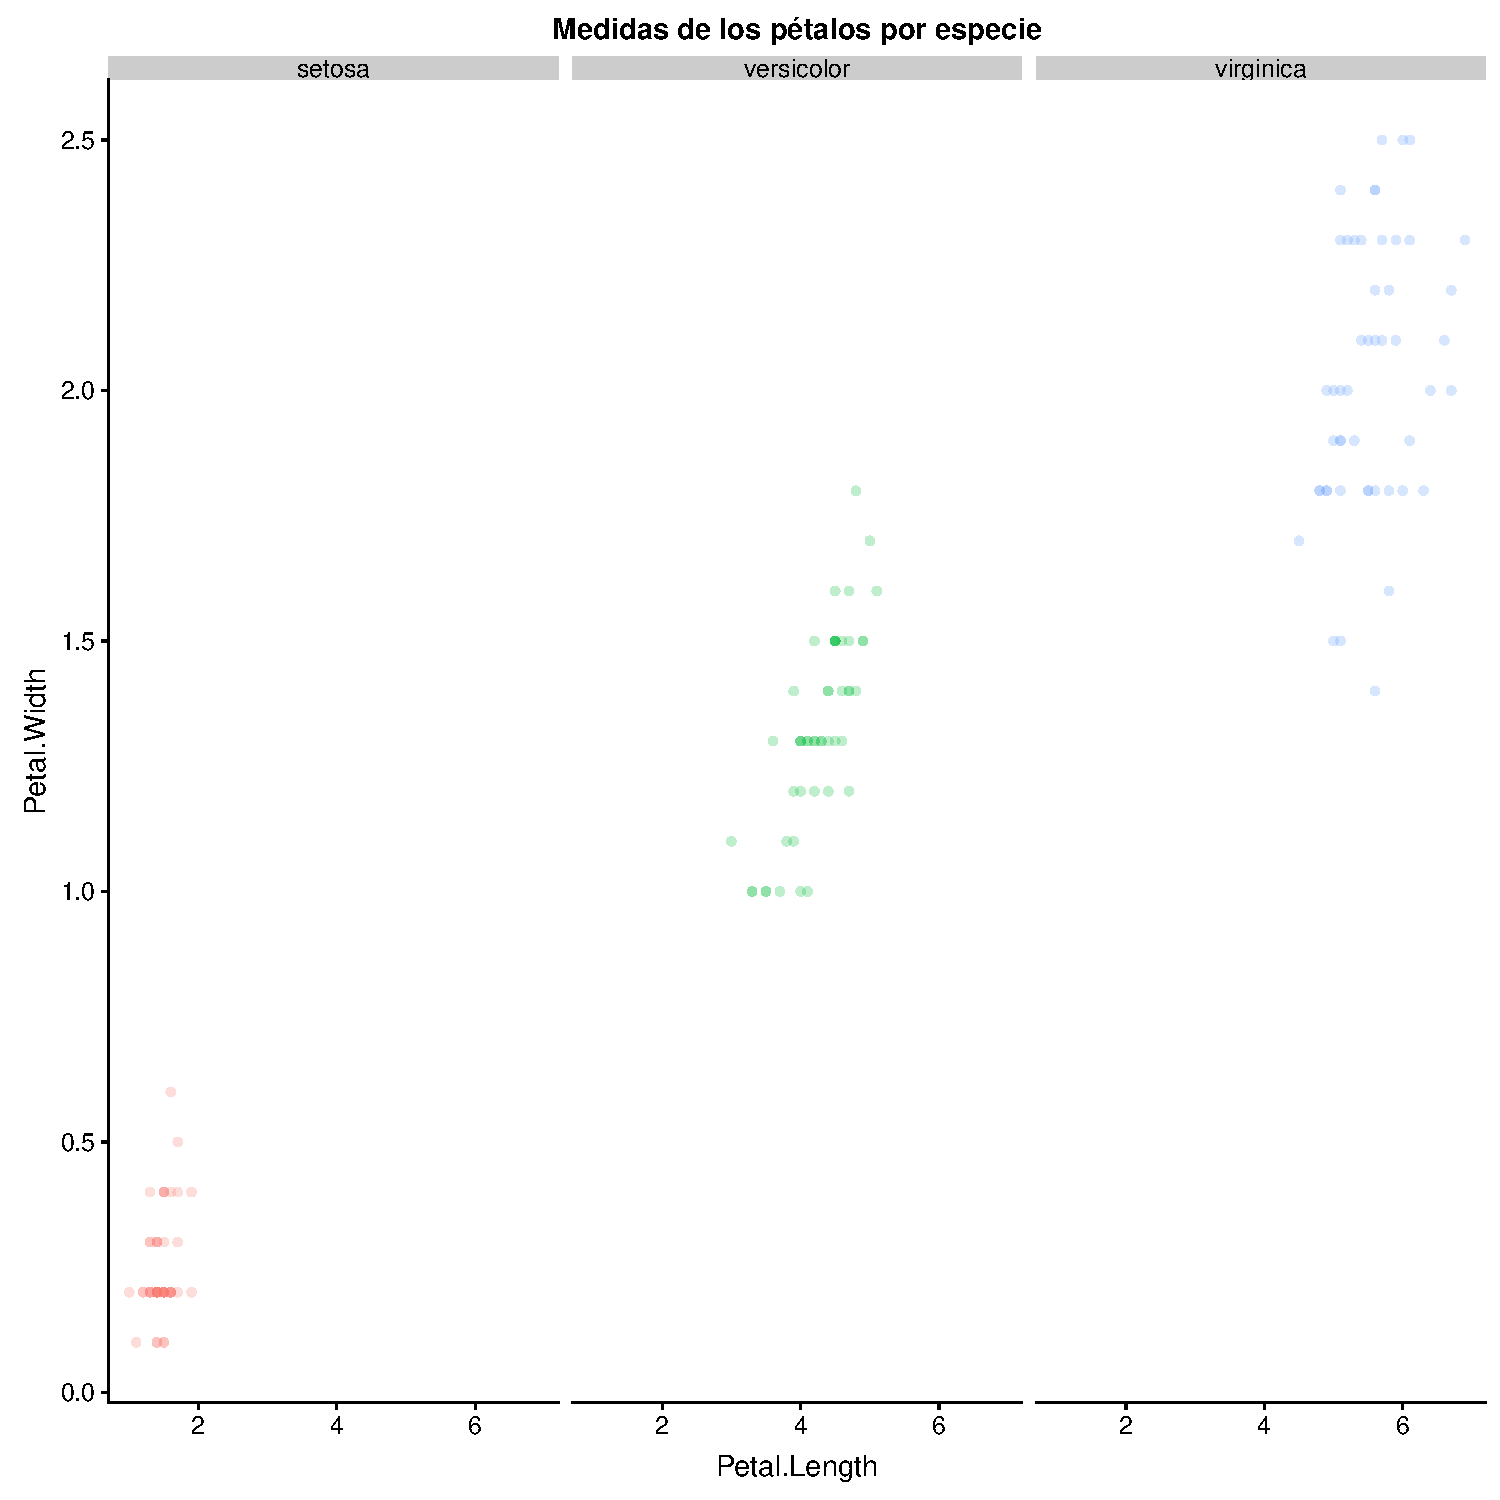
\includegraphics{bookdown_files/figure-latex/unnamed-chunk-80-1.pdf}

\hypertarget{extensiones-de-ggplot.}{%
\subsubsection{\texorpdfstring{Extensiones de \href{http://www.ggplot2-exts.org/gallery/}{GGplot}.}{Extensiones de GGplot.}}\label{extensiones-de-ggplot.}}

La librería GGplot tiene a su vez muchas otras librerías que extienden sus potencialidades. Entre nuestras favoritas están:

\begin{itemize}
\tightlist
\item
  \href{https://gganimate.com/}{gganimate}: Para hacer gráficos animados.
\item
  \href{https://cran.r-project.org/web/packages/ggridges/vignettes/introduction.html}{ggridge}: Para hacer gráficos de densidad faceteados
\item
  \href{https://ggobi.github.io/ggally/}{ggally}: Para hacer varios gráficos juntos.
  \^{}
\end{itemize}

\begin{Shaded}
\begin{Highlighting}[]
\KeywordTok{library}\NormalTok{(GGally)}

\KeywordTok{ggpairs}\NormalTok{(iris,  }\DataTypeTok{mapping =} \KeywordTok{aes}\NormalTok{(}\DataTypeTok{color =}\NormalTok{ Species))}
\end{Highlighting}
\end{Shaded}

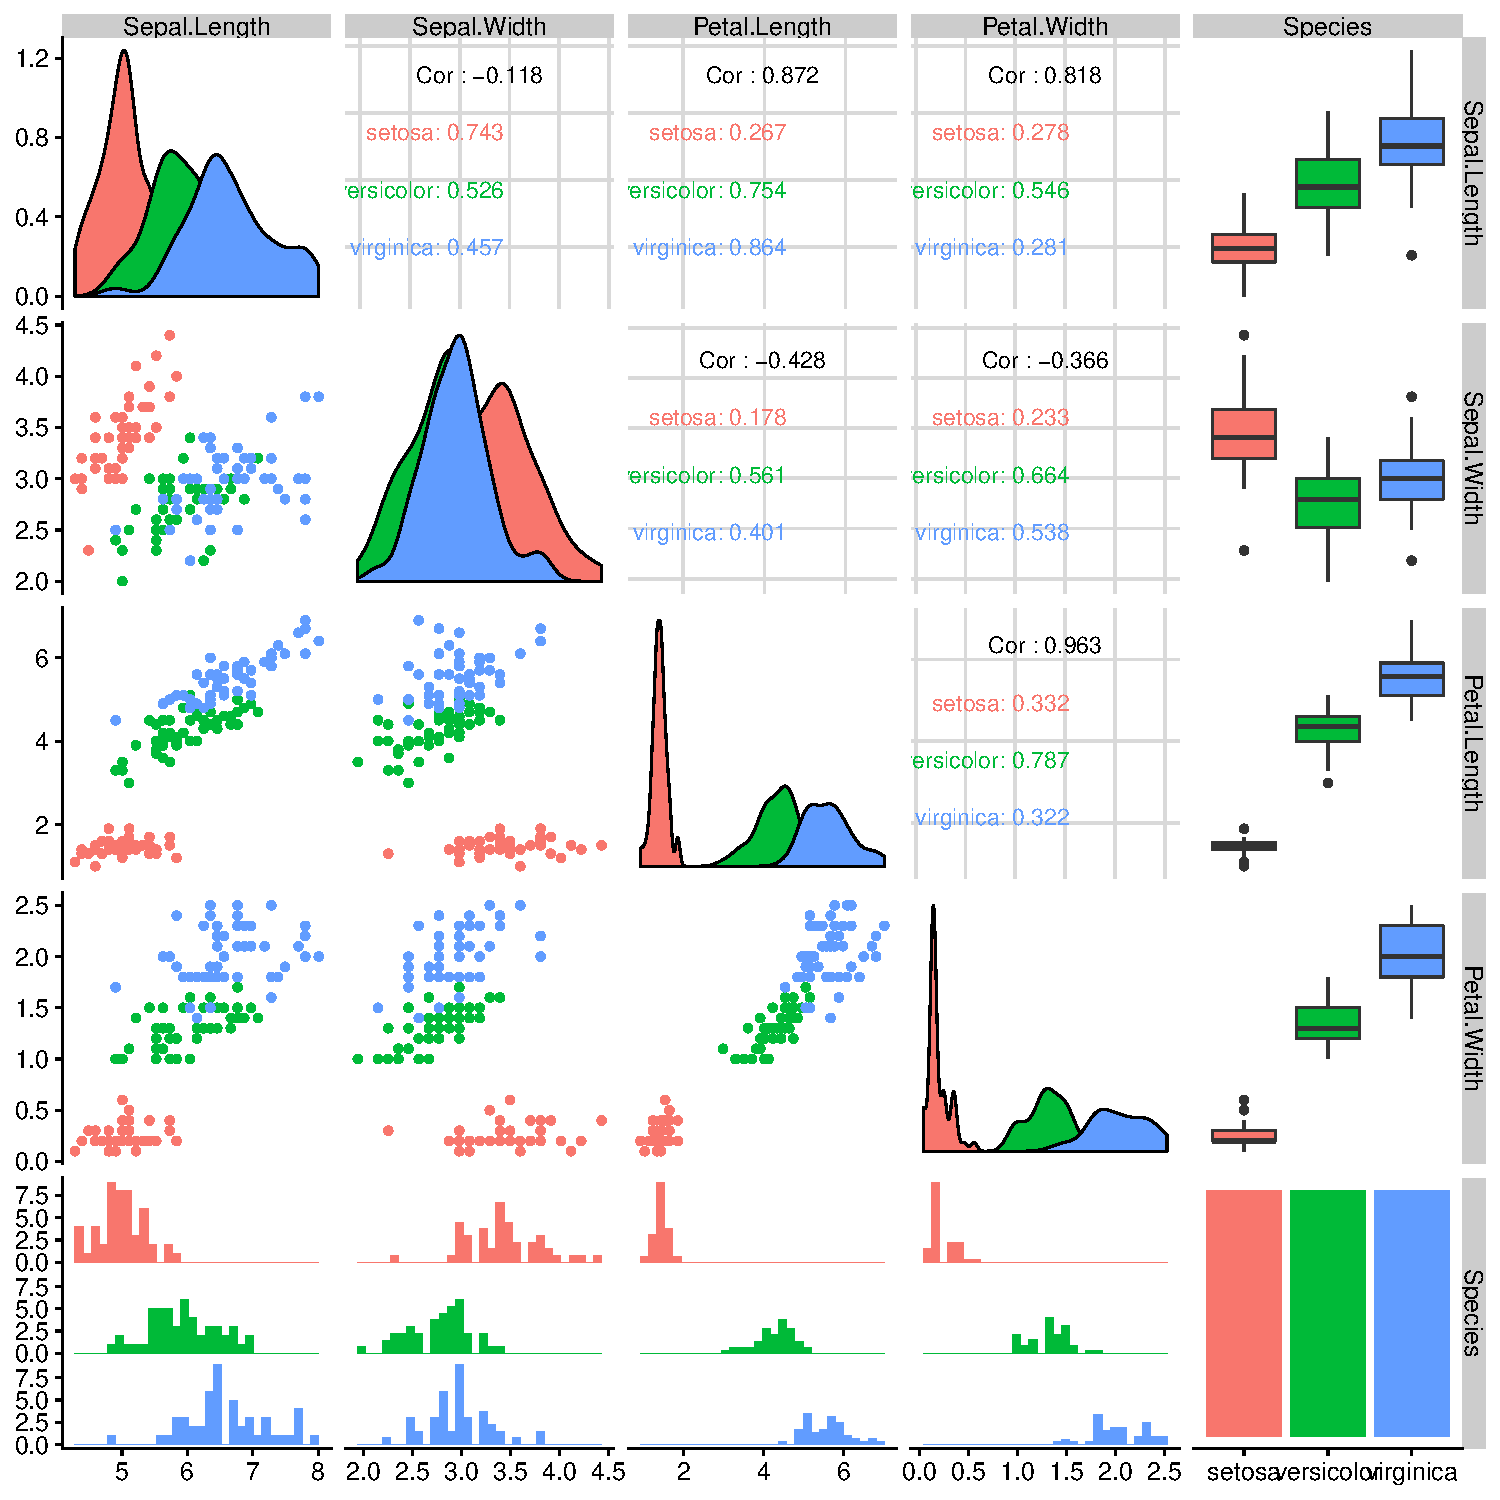
\includegraphics{bookdown_files/figure-latex/unnamed-chunk-81-1.pdf}

\begin{Shaded}
\begin{Highlighting}[]
\KeywordTok{library}\NormalTok{(ggridges)}
\KeywordTok{ggplot}\NormalTok{(iris, }\KeywordTok{aes}\NormalTok{(}\DataTypeTok{x =}\NormalTok{ Sepal.Length, }\DataTypeTok{y =}\NormalTok{ Species, }\DataTypeTok{fill=}\NormalTok{Species)) }\OperatorTok{+}\StringTok{ }
\StringTok{  }\KeywordTok{geom_density_ridges}\NormalTok{()}
\end{Highlighting}
\end{Shaded}

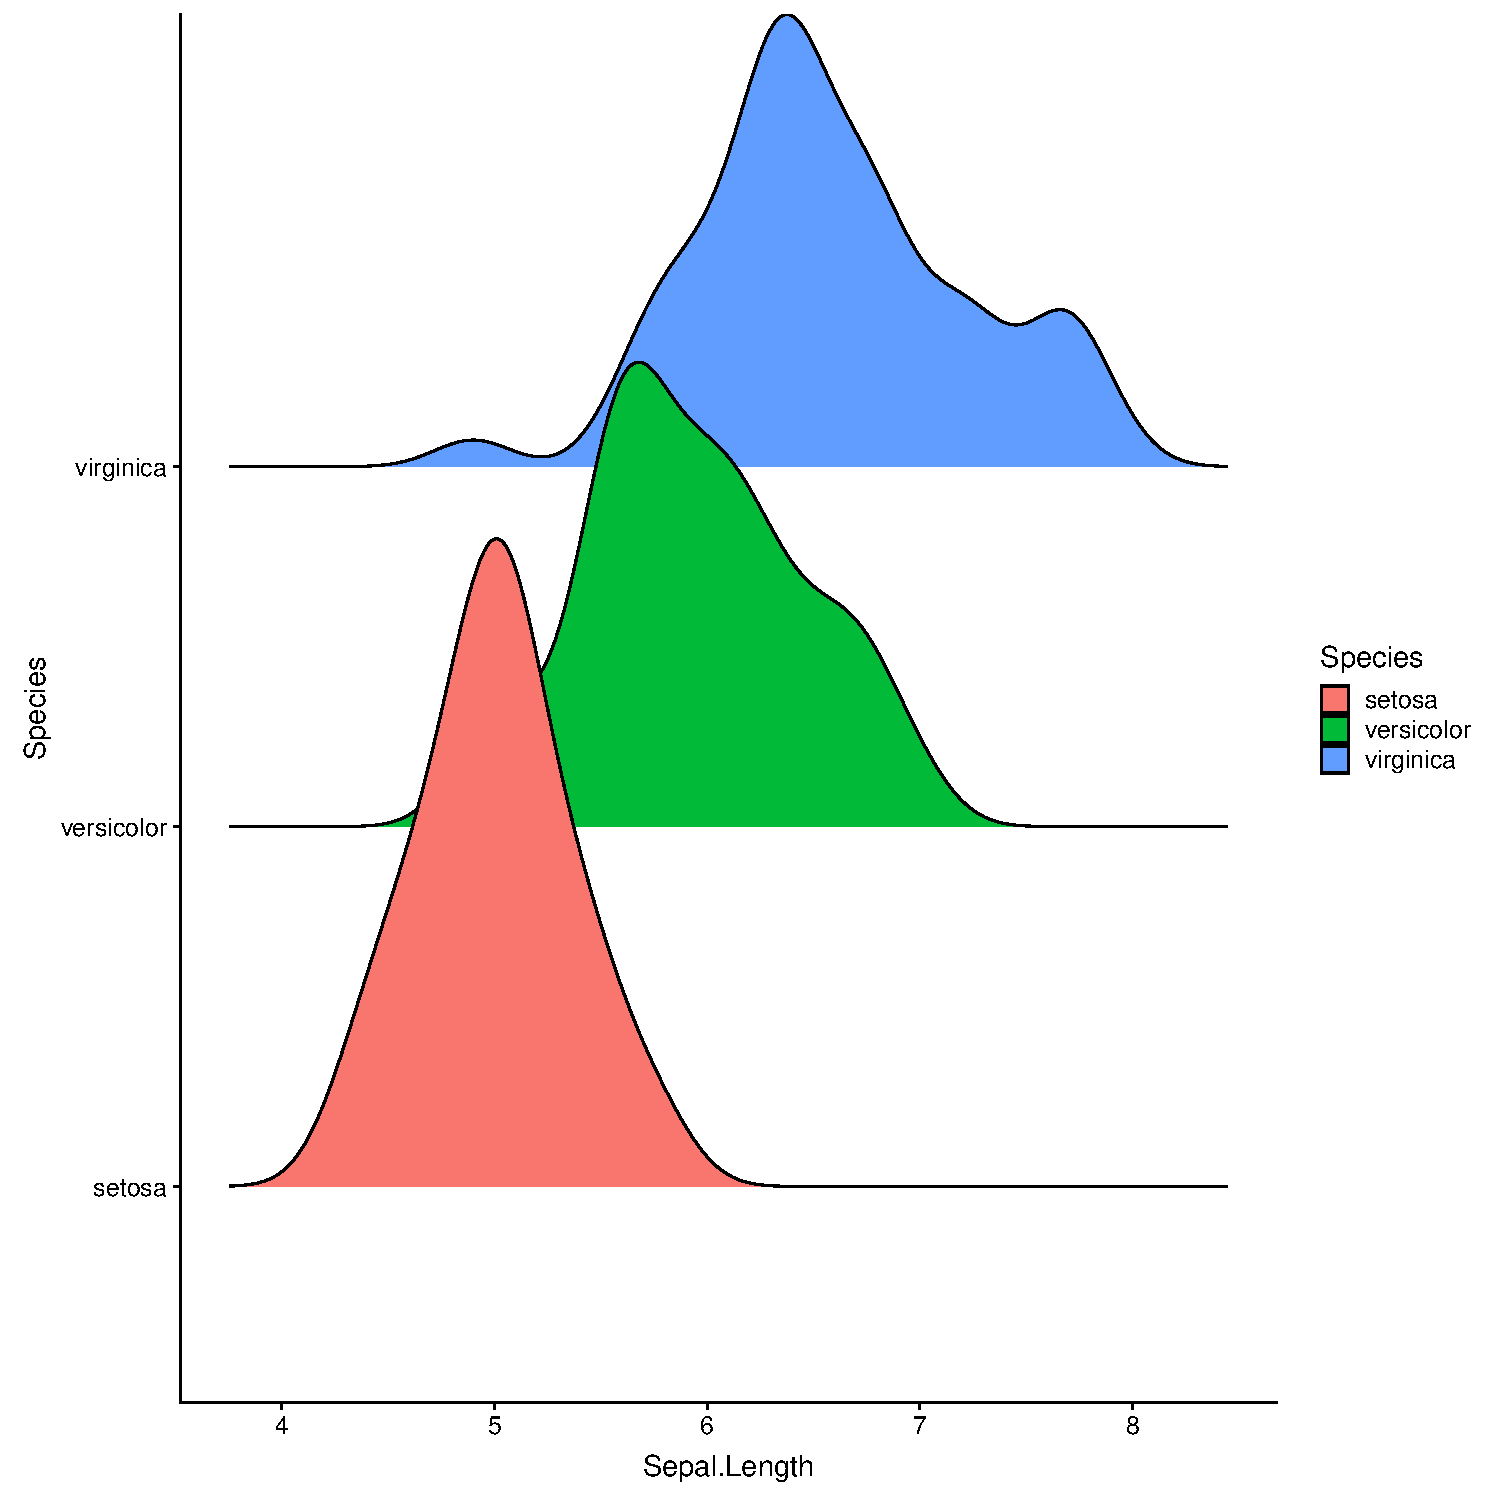
\includegraphics{bookdown_files/figure-latex/unnamed-chunk-82-1.pdf}

También hay extensiones que te ayudan a escribir el código, como \href{https://dreamrs.github.io/esquisse/}{esquisse}

\begin{Shaded}
\begin{Highlighting}[]
\NormalTok{iris <-}\StringTok{ }\NormalTok{iris}
\CommentTok{#Correr en la consola}
\NormalTok{esquisse}\OperatorTok{::}\KeywordTok{esquisser}\NormalTok{()}
\end{Highlighting}
\end{Shaded}

\hypertarget{dimensiones-del-grafico}{%
\subsection{Dimensiones del gráfico}\label{dimensiones-del-grafico}}

Esta forma de pensar los gráficos nos permite repenser los distintos atributos como potenciales aliados a la hora de mostrar información multidimensional. Por ejemplo:

\begin{itemize}
\item
  \href{http://www.stat.columbia.edu/~tzheng/files/Rcolor.pdf}{\textbf{color}} \texttt{color\ =}
\item
  \textbf{relleno}\texttt{fill\ =}
\item
  \textbf{forma} \texttt{shape\ =}
\item
  \textbf{tamaño} \texttt{size\ =}
\item
  \textbf{transparencia} \texttt{alpha\ =}
\item
  Abrir un mismo gráfico según alguna variable discreta: \texttt{facet\_wrap()}
\item
  Los atributos que queremos que \emph{mapeen} una variable, deben ir \textbf{dentro del aes()}, \texttt{aes(...\ color\ =\ variable)}
\item
  Cuando queremos simplemente mejorar el diseño (es fijo), se asigna por fuera, o dentro de cada tipo de gráficos, \texttt{geom\_col(color\ =\ \textquotesingle{}green\textquotesingle{})}.
\end{itemize}

\hypertarget{treemaps}{%
\subsection{Treemaps}\label{treemaps}}

\begin{Shaded}
\begin{Highlighting}[]
\KeywordTok{library}\NormalTok{(treemapify)}
\end{Highlighting}
\end{Shaded}

\href{https://data.buenosaires.gob.ar/dataset/trabajo-domestico-no-remunerado}{Trabajo doméstico no remunerado}

\begin{Shaded}
\begin{Highlighting}[]
\NormalTok{trabajo_no_remunerado <-}\StringTok{ }\KeywordTok{read_csv}\NormalTok{(}\StringTok{'fuentes/prom_t_simul_dom_16_sexo__annio__g_edad_limpio.csv'}\NormalTok{)}
\end{Highlighting}
\end{Shaded}

\begin{Shaded}
\begin{Highlighting}[]
\NormalTok{ trabajo_no_remunerado }\OperatorTok\StringTok{ }
\StringTok{  }\KeywordTok{filter}\NormalTok{(sexo }\OperatorTok{!=}\StringTok{ 'TOTAL'}\NormalTok{, grupo_edad }\OperatorTok{!=}\StringTok{ 'TOTAL'}\NormalTok{) }\OperatorTok
\StringTok{   }\KeywordTok{mutate}\NormalTok{(}\DataTypeTok{promedio_hs_diarias =} \KeywordTok{as.numeric}\NormalTok{(promedio_hs_diarias),}
          \DataTypeTok{sexo =} \KeywordTok{case_when}\NormalTok{(sexo}\OperatorTok{==}\StringTok{'m'}\OperatorTok{~}\StringTok{'Mujer'}\NormalTok{,}
\NormalTok{                           sexo}\OperatorTok{==}\StringTok{'v'}\OperatorTok{~}\StringTok{'Varón')) %>% }
\StringTok{  ggplot(., aes(area = promedio_hs_diarias, fill = promedio_hs_diarias, label = grupo_edad,}
\StringTok{                subgroup = sexo)) +}
\StringTok{  geom_treemap() +}
\StringTok{  geom_treemap_subgroup_border() +}
\StringTok{  geom_treemap_subgroup_text(place = "centre", grow = T, alpha = 0.5, colour =}
\StringTok{                             "black", fontface = "italic", min.size = 0) +}
\StringTok{  geom_treemap_text(colour = "white", place = "topleft", reflow = T)+}
\StringTok{  theme(legend.position = '}\NormalTok{none}\StringTok{')}
\end{Highlighting}
\end{Shaded}

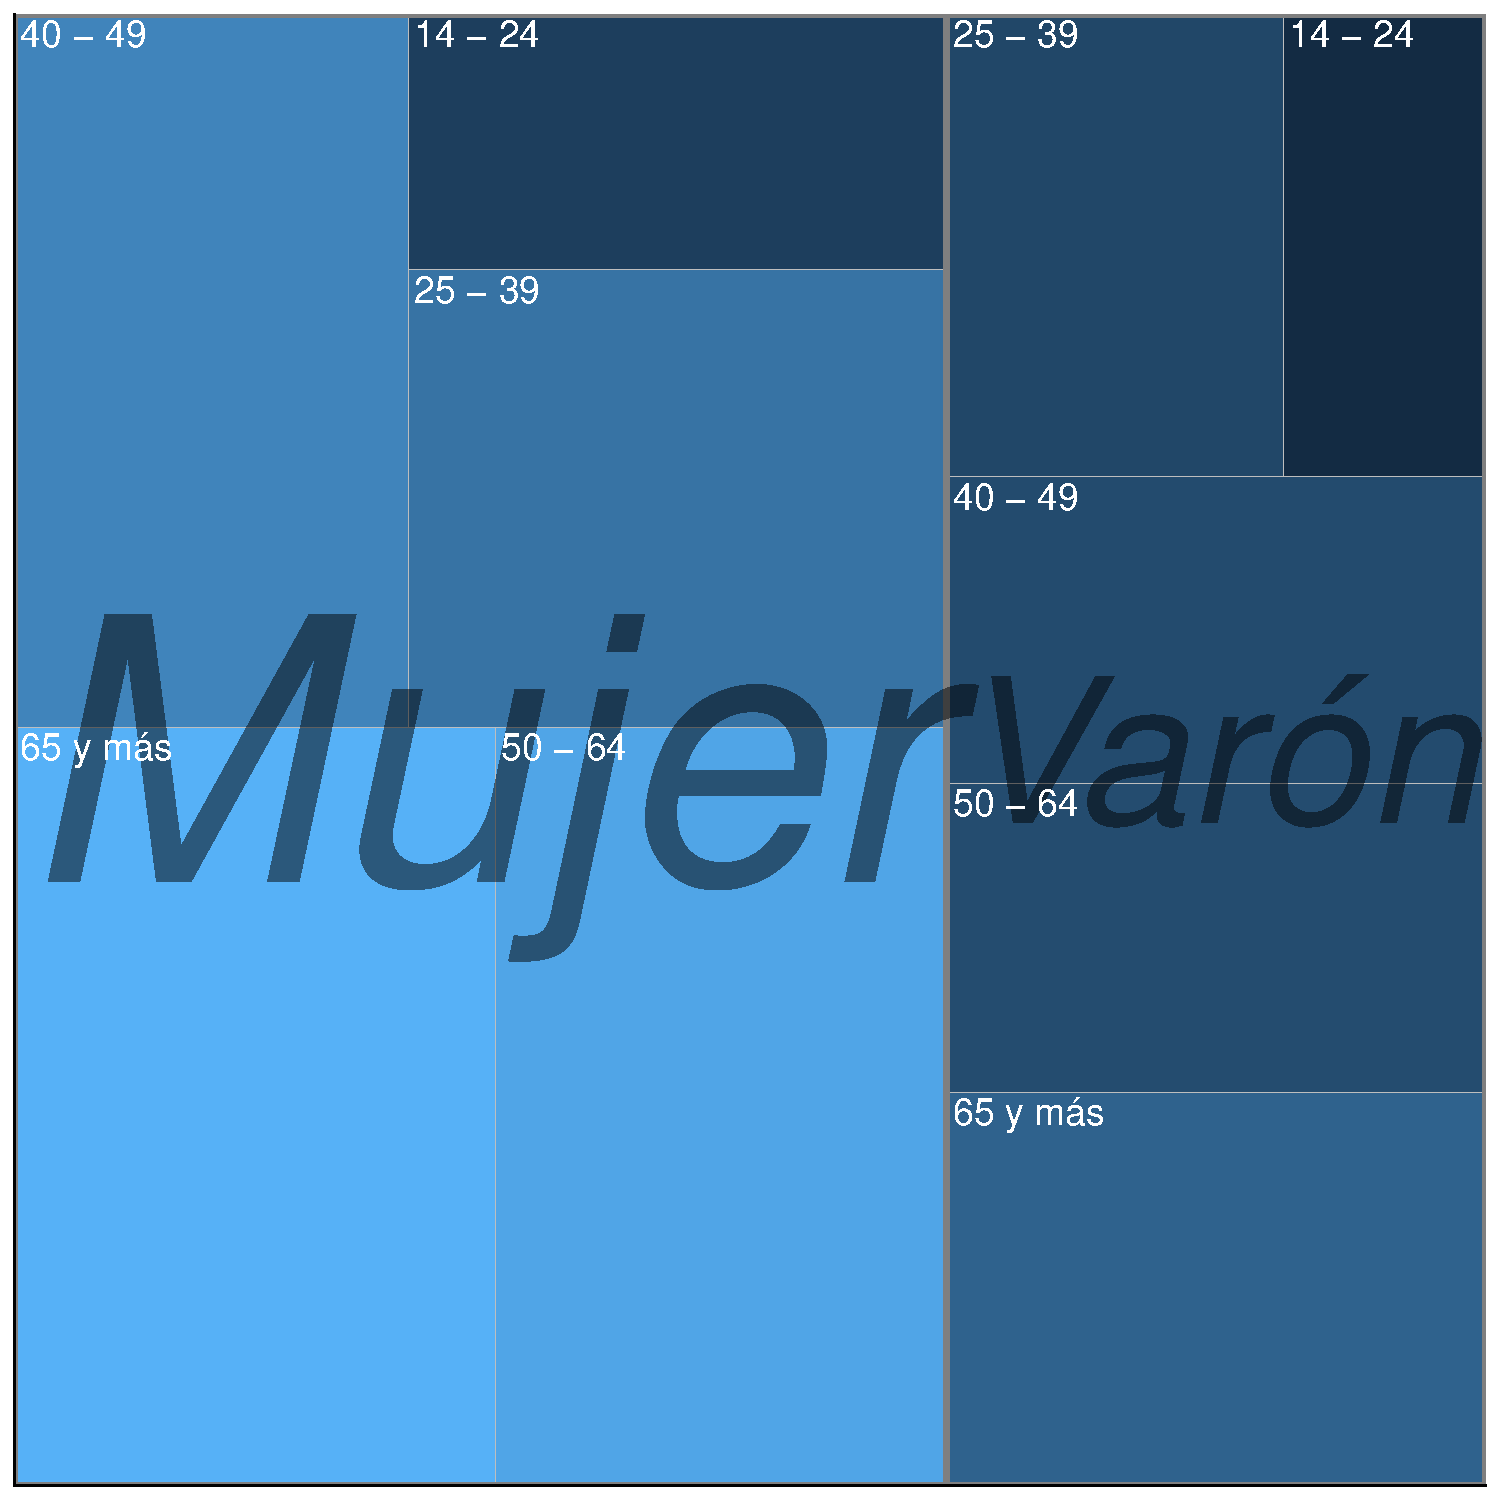
\includegraphics{bookdown_files/figure-latex/unnamed-chunk-86-1.pdf}

\begin{Shaded}
\begin{Highlighting}[]
\NormalTok{ trabajo_no_remunerado }\OperatorTok\StringTok{ }
\StringTok{  }\KeywordTok{filter}\NormalTok{(sexo }\OperatorTok{!=}\StringTok{ 'TOTAL'}\NormalTok{, grupo_edad }\OperatorTok{!=}\StringTok{ 'TOTAL'}\NormalTok{) }\OperatorTok
\StringTok{   }\KeywordTok{mutate}\NormalTok{(}\DataTypeTok{promedio_hs_diarias =} \KeywordTok{as.numeric}\NormalTok{(promedio_hs_diarias)) }\OperatorTok\StringTok{ }
\KeywordTok{ggplot}\NormalTok{(., }\KeywordTok{aes}\NormalTok{(}\DataTypeTok{area=}\NormalTok{promedio_hs_diarias, }\DataTypeTok{fill=}\NormalTok{sexo, }\DataTypeTok{label=}\NormalTok{sexo))}\OperatorTok{+}
\StringTok{  }\KeywordTok{geom_treemap}\NormalTok{() }\OperatorTok{+}
\StringTok{  }\KeywordTok{geom_treemap_text}\NormalTok{(}\DataTypeTok{colour =} \StringTok{"white"}\NormalTok{, }\DataTypeTok{place =} \StringTok{"topleft"}\NormalTok{, }\DataTypeTok{reflow =}\NormalTok{ T)}\OperatorTok{+}
\StringTok{  }\KeywordTok{facet_wrap}\NormalTok{(.}\OperatorTok{~}\NormalTok{grupo_edad, }\DataTypeTok{ncol =} \DecValTok{1}\NormalTok{)}
\end{Highlighting}
\end{Shaded}

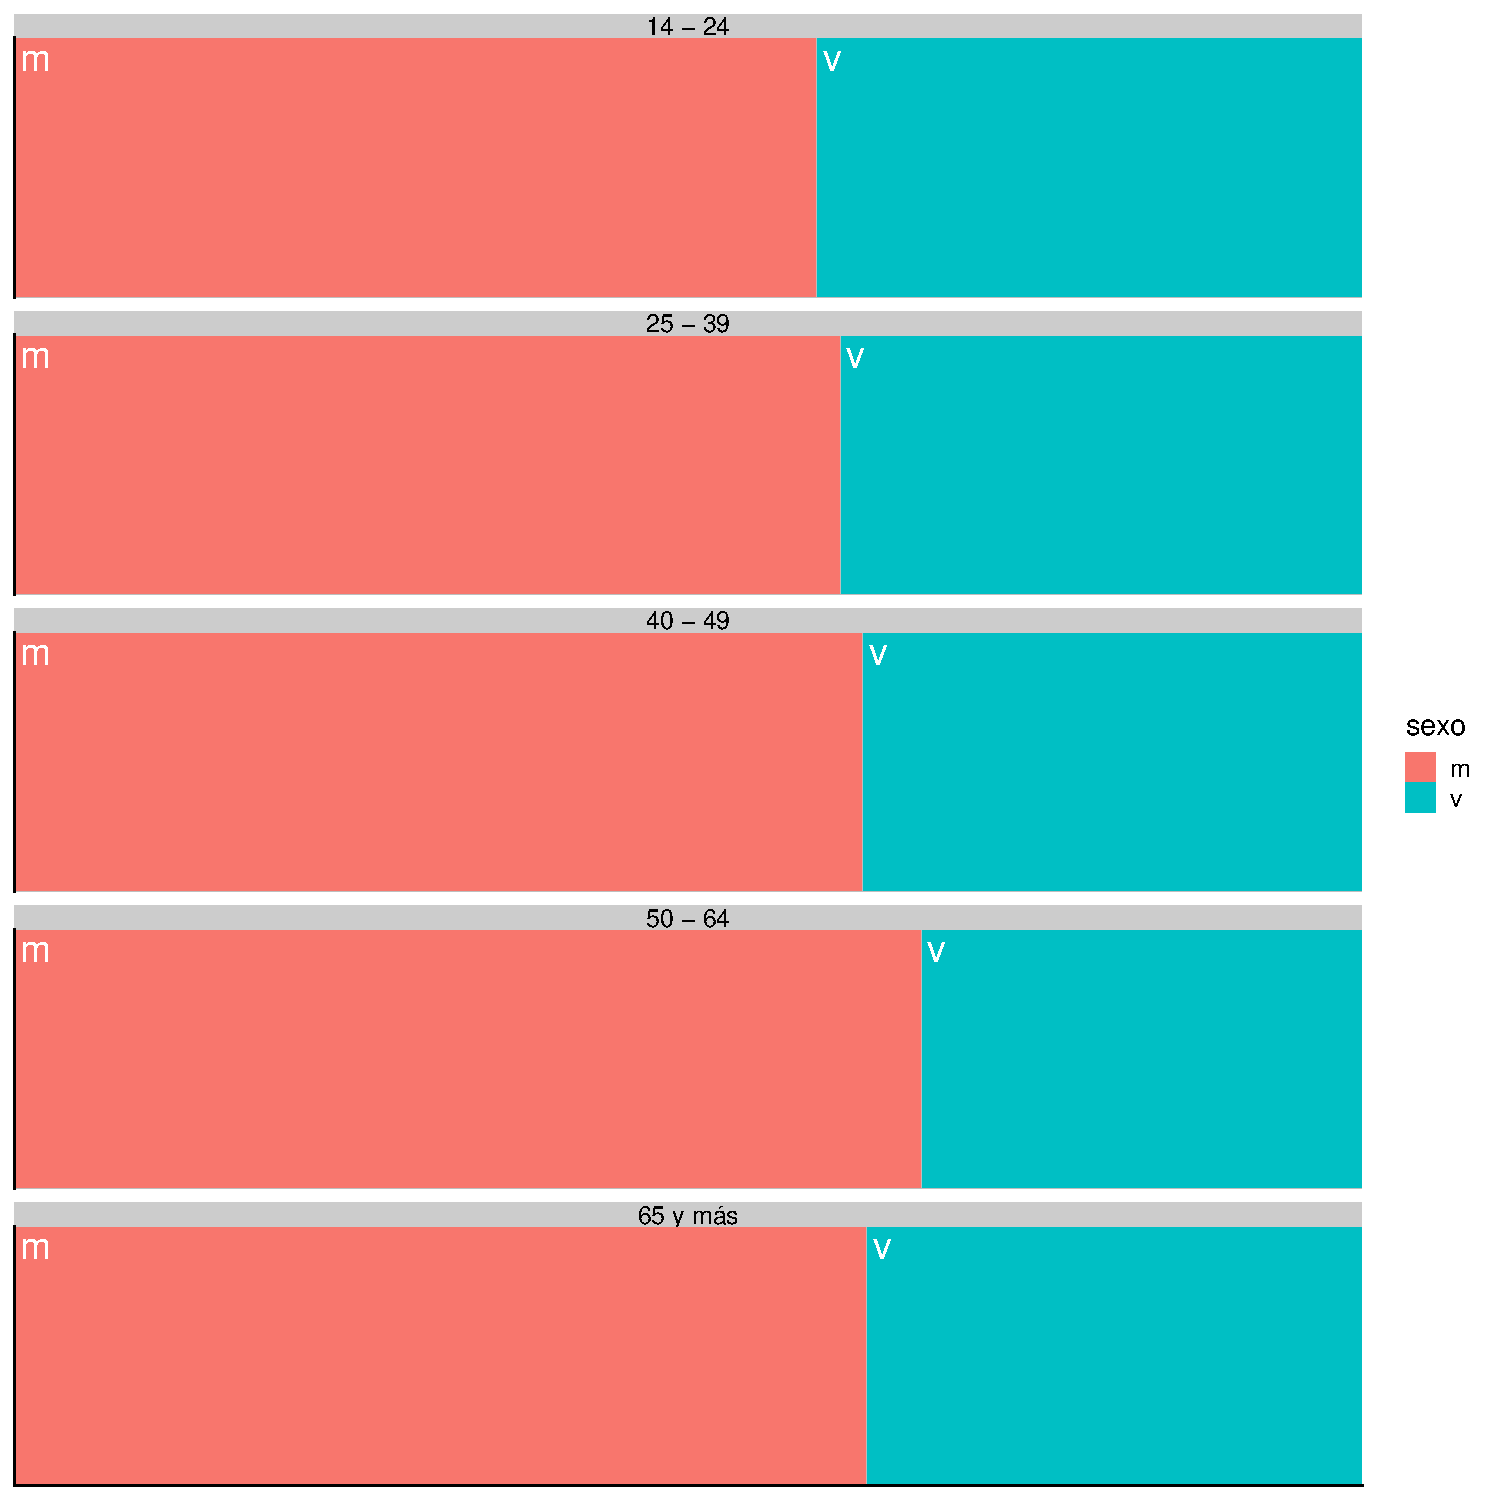
\includegraphics{bookdown_files/figure-latex/unnamed-chunk-87-1.pdf}

\hypertarget{practica-guiada-2}{%
\section{Práctica Guiada}\label{practica-guiada-2}}

\hypertarget{graficos-ingresos---eph}{%
\subsection{Graficos Ingresos - EPH}\label{graficos-ingresos---eph}}

Para esta práctica utilizaremos las variables de ingresos captadas por la \href{https://www.indec.gob.ar/indec/web/Institucional-Indec-BasesDeDatos}{Encuesta Permanente de Hogares}

A continuación utilzaremos los conceptos abordados, para realizar gráficos a partir de las variables de ingresos.

\begin{Shaded}
\begin{Highlighting}[]
\CommentTok{#Cargamos las librerías a utilizar}

\KeywordTok{library}\NormalTok{(tidyverse) }\CommentTok{# tiene ggplot, dplyr, tidyr, y otros}
\KeywordTok{library}\NormalTok{(ggthemes)  }\CommentTok{# estilos de gráficos}
\KeywordTok{library}\NormalTok{(ggrepel)   }\CommentTok{# etiquetas de texto más prolijas que las de ggplot}
\end{Highlighting}
\end{Shaded}

\begin{Shaded}
\begin{Highlighting}[]

\NormalTok{Individual_t119 <-}\StringTok{ }\KeywordTok{read.table}\NormalTok{(}\StringTok{"fuentes/usu_individual_t119.txt"}\NormalTok{,}
                              \DataTypeTok{sep=}\StringTok{";"}\NormalTok{, }\DataTypeTok{dec=}\StringTok{","}\NormalTok{, }\DataTypeTok{header =} \OtherTok{TRUE}\NormalTok{, }\DataTypeTok{fill =} \OtherTok{TRUE}\NormalTok{)}
\end{Highlighting}
\end{Shaded}

\hypertarget{boxplot-de-ingresos-de-la-ocupacion-principal-segun-nivel-educativo}{%
\subsubsection{Boxplot de ingresos de la ocupación principal, según nivel educativo}\label{boxplot-de-ingresos-de-la-ocupacion-principal-segun-nivel-educativo}}

Hacemos un procesamiento simple: Sacamos los ingresos iguales a cero y las no respuestas de nivel educativo.\\
Es importante que las variables sean del tipo que conceptualmente les corresponde (el nivel educativo es una variable categórica, no continua), para que el ggplot pueda graficarlo correctamente.

\begin{Shaded}
\begin{Highlighting}[]
\CommentTok{# Las variables sexo( CH04 ) y Nivel educativo están codificadas como números, y el R las entiende como numéricas.}
\KeywordTok{class}\NormalTok{(Individual_t119}\OperatorTok{$}\NormalTok{NIVEL_ED)}
\end{Highlighting}
\end{Shaded}

\begin{verbatim}
## [1] "integer"
\end{verbatim}

\begin{Shaded}
\begin{Highlighting}[]
\KeywordTok{class}\NormalTok{(Individual_t119}\OperatorTok{$}\NormalTok{CH04)}
\end{Highlighting}
\end{Shaded}

\begin{verbatim}
## [1] "integer"
\end{verbatim}

\begin{Shaded}
\begin{Highlighting}[]
\NormalTok{ggdata <-}\StringTok{ }\NormalTok{Individual_t119 }\OperatorTok\StringTok{ }
\StringTok{  }\KeywordTok{filter}\NormalTok{(P21}\OperatorTok{>}\DecValTok{0}\NormalTok{, }\OperatorTok{!}\KeywordTok{is.na}\NormalTok{(NIVEL_ED)) }\OperatorTok\StringTok{ }
\StringTok{  }\KeywordTok{mutate}\NormalTok{(}\DataTypeTok{NIVEL_ED =} \KeywordTok{as.factor}\NormalTok{(NIVEL_ED),}
         \DataTypeTok{CH04     =} \KeywordTok{as.factor}\NormalTok{(CH04))}
\end{Highlighting}
\end{Shaded}

\begin{Shaded}
\begin{Highlighting}[]
\KeywordTok{ggplot}\NormalTok{(ggdata, }\KeywordTok{aes}\NormalTok{(}\DataTypeTok{x =}\NormalTok{ NIVEL_ED, }\DataTypeTok{y =}\NormalTok{ P21)) }\OperatorTok{+}
\StringTok{  }\KeywordTok{geom_boxplot}\NormalTok{()}\OperatorTok{+}
\StringTok{  }\KeywordTok{scale_y_continuous}\NormalTok{(}\DataTypeTok{limits =} \KeywordTok{c}\NormalTok{(}\DecValTok{0}\NormalTok{, }\DecValTok{40000}\NormalTok{))}\CommentTok{#Restrinjo el gráfico hasta ingresos de $40000}
\end{Highlighting}
\end{Shaded}

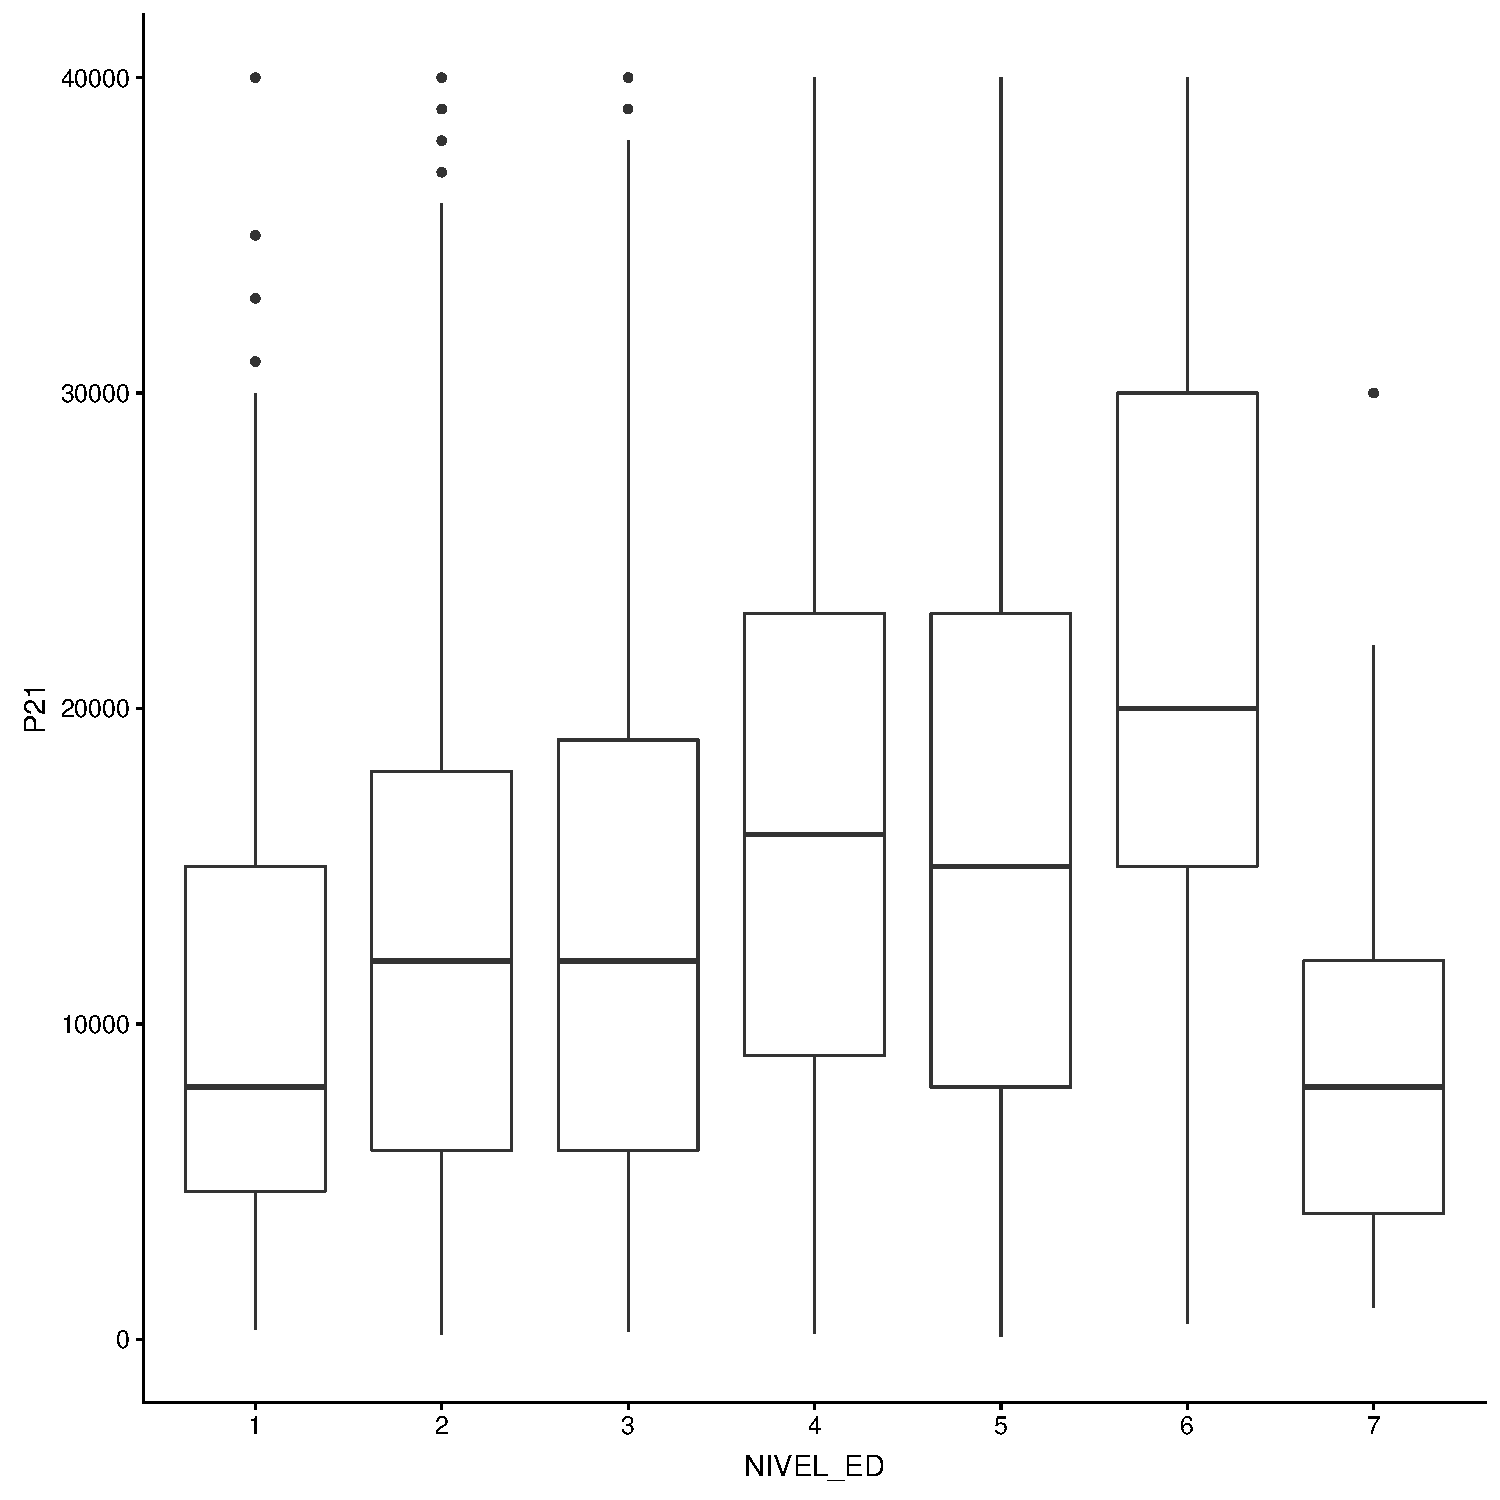
\includegraphics{bookdown_files/figure-latex/unnamed-chunk-91-1.pdf}

Si queremos agregar la dimensión \emph{sexo}, podemos hacer un \texttt{facet\_wrap()}

\begin{Shaded}
\begin{Highlighting}[]
\KeywordTok{ggplot}\NormalTok{(ggdata, }\KeywordTok{aes}\NormalTok{(}\DataTypeTok{x=}\NormalTok{ NIVEL_ED, }\DataTypeTok{y =}\NormalTok{ P21, }\DataTypeTok{group =}\NormalTok{ NIVEL_ED, }\DataTypeTok{fill =}\NormalTok{ NIVEL_ED )) }\OperatorTok{+}
\StringTok{  }\KeywordTok{geom_boxplot}\NormalTok{()}\OperatorTok{+}
\StringTok{  }\KeywordTok{scale_y_continuous}\NormalTok{(}\DataTypeTok{limits =} \KeywordTok{c}\NormalTok{(}\DecValTok{0}\NormalTok{, }\DecValTok{40000}\NormalTok{))}\OperatorTok{+}
\StringTok{  }\KeywordTok{facet_wrap}\NormalTok{(}\OperatorTok{~}\StringTok{ }\NormalTok{CH04, }\DataTypeTok{labeller =} \StringTok{"label_both"}\NormalTok{)}
\end{Highlighting}
\end{Shaded}

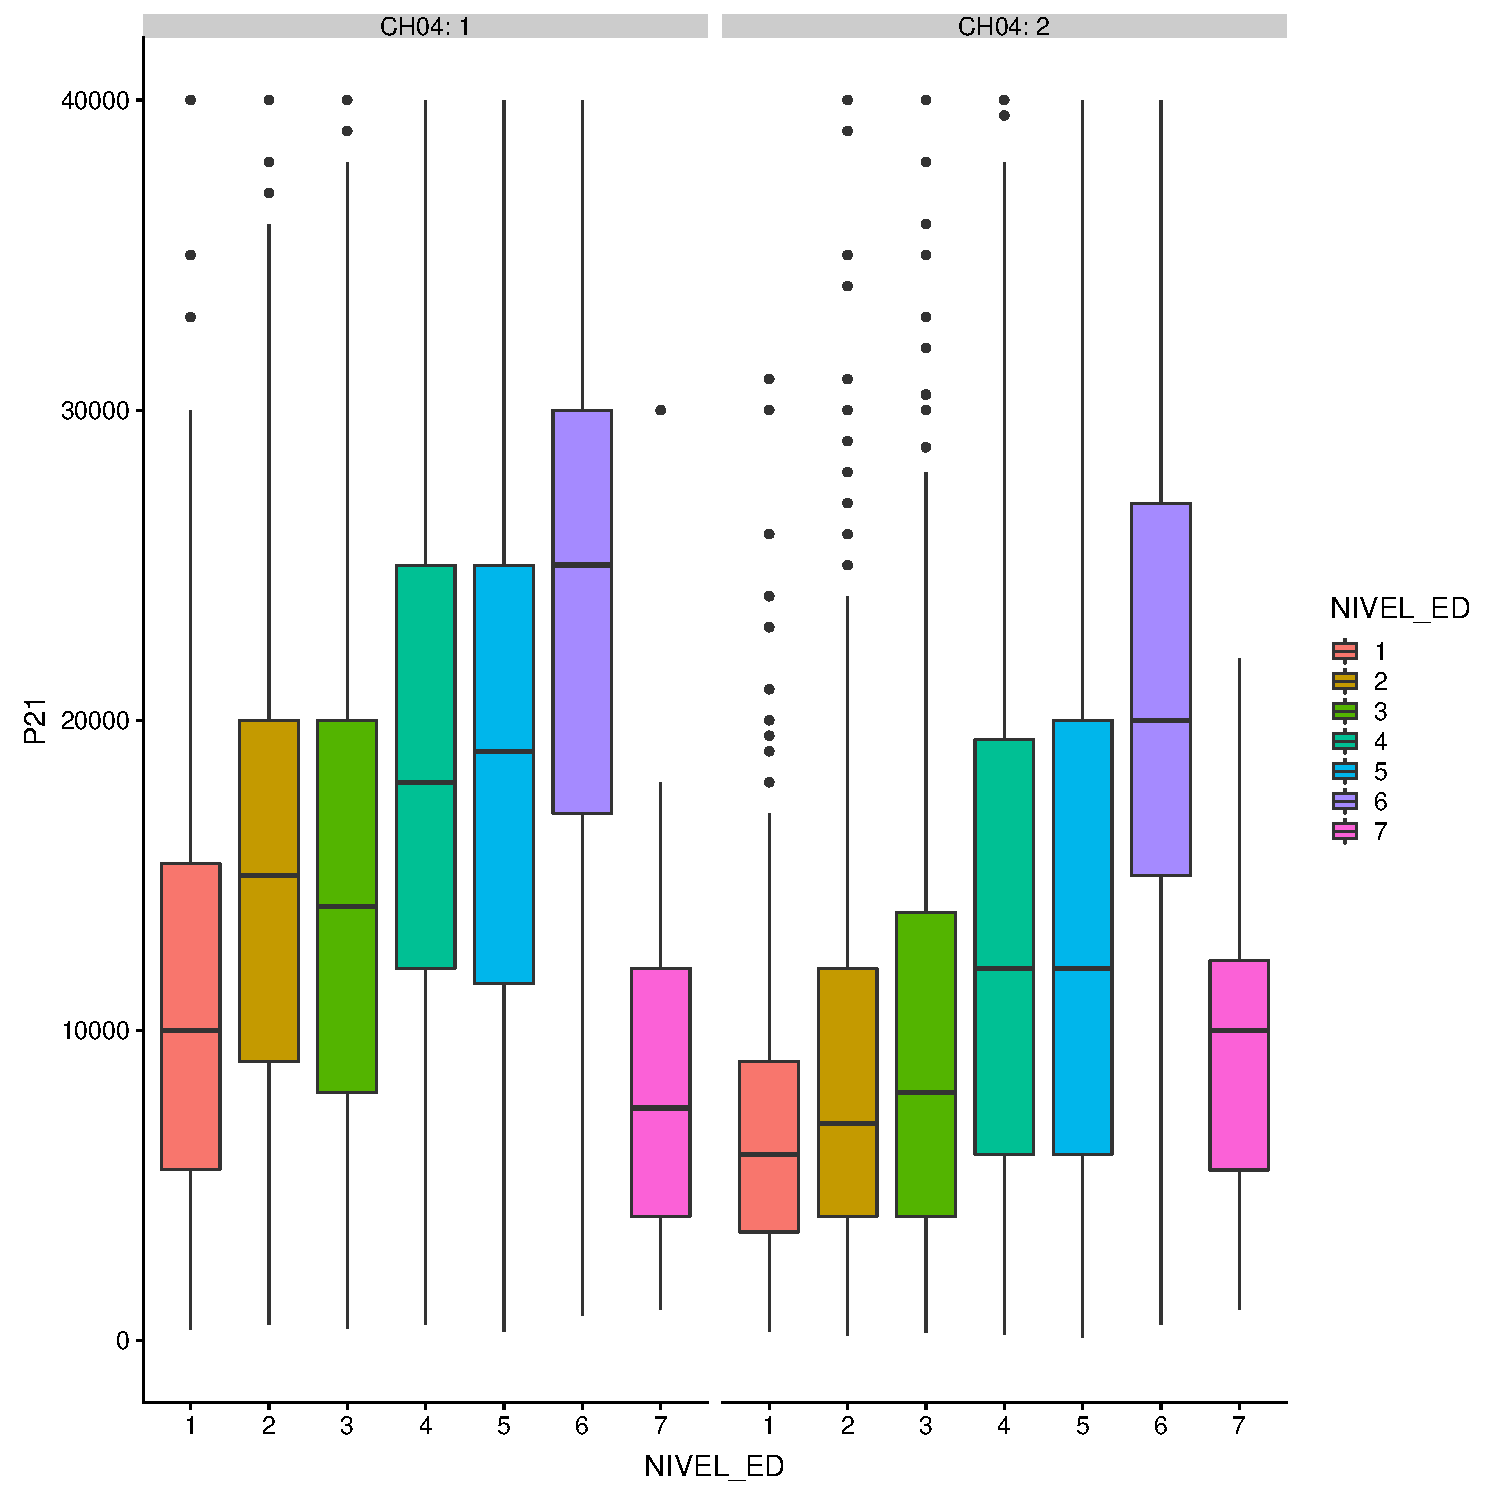
\includegraphics{bookdown_files/figure-latex/unnamed-chunk-92-1.pdf}

Por la forma en que está presentado el gráfico, el foco de atención sigue puesto en las diferencias de ingresos entre niveles educativo. Simplemente se agrega un corte por la variable de sexo.

Si lo que queremos hacer es poner el foco de atención en las diferencias por sexo, simplemente basta con invertir la variable x especificada con la variable utilizada en el \texttt{facet\_wrap}

\begin{Shaded}
\begin{Highlighting}[]
\KeywordTok{ggplot}\NormalTok{(ggdata, }\KeywordTok{aes}\NormalTok{(}\DataTypeTok{x=}\NormalTok{ CH04, }\DataTypeTok{y =}\NormalTok{ P21, }\DataTypeTok{group =}\NormalTok{ CH04, }\DataTypeTok{fill =}\NormalTok{ CH04 )) }\OperatorTok{+}
\StringTok{  }\KeywordTok{geom_boxplot}\NormalTok{()}\OperatorTok{+}
\StringTok{  }\KeywordTok{scale_y_continuous}\NormalTok{(}\DataTypeTok{limits =} \KeywordTok{c}\NormalTok{(}\DecValTok{0}\NormalTok{, }\DecValTok{40000}\NormalTok{))}\OperatorTok{+}
\StringTok{  }\KeywordTok{facet_grid}\NormalTok{(}\OperatorTok{~}\StringTok{ }\NormalTok{NIVEL_ED, }\DataTypeTok{labeller =} \StringTok{"label_both"}\NormalTok{) }\OperatorTok{+}
\StringTok{  }\KeywordTok{theme}\NormalTok{(}\DataTypeTok{legend.position =} \StringTok{"none"}\NormalTok{)}
\end{Highlighting}
\end{Shaded}

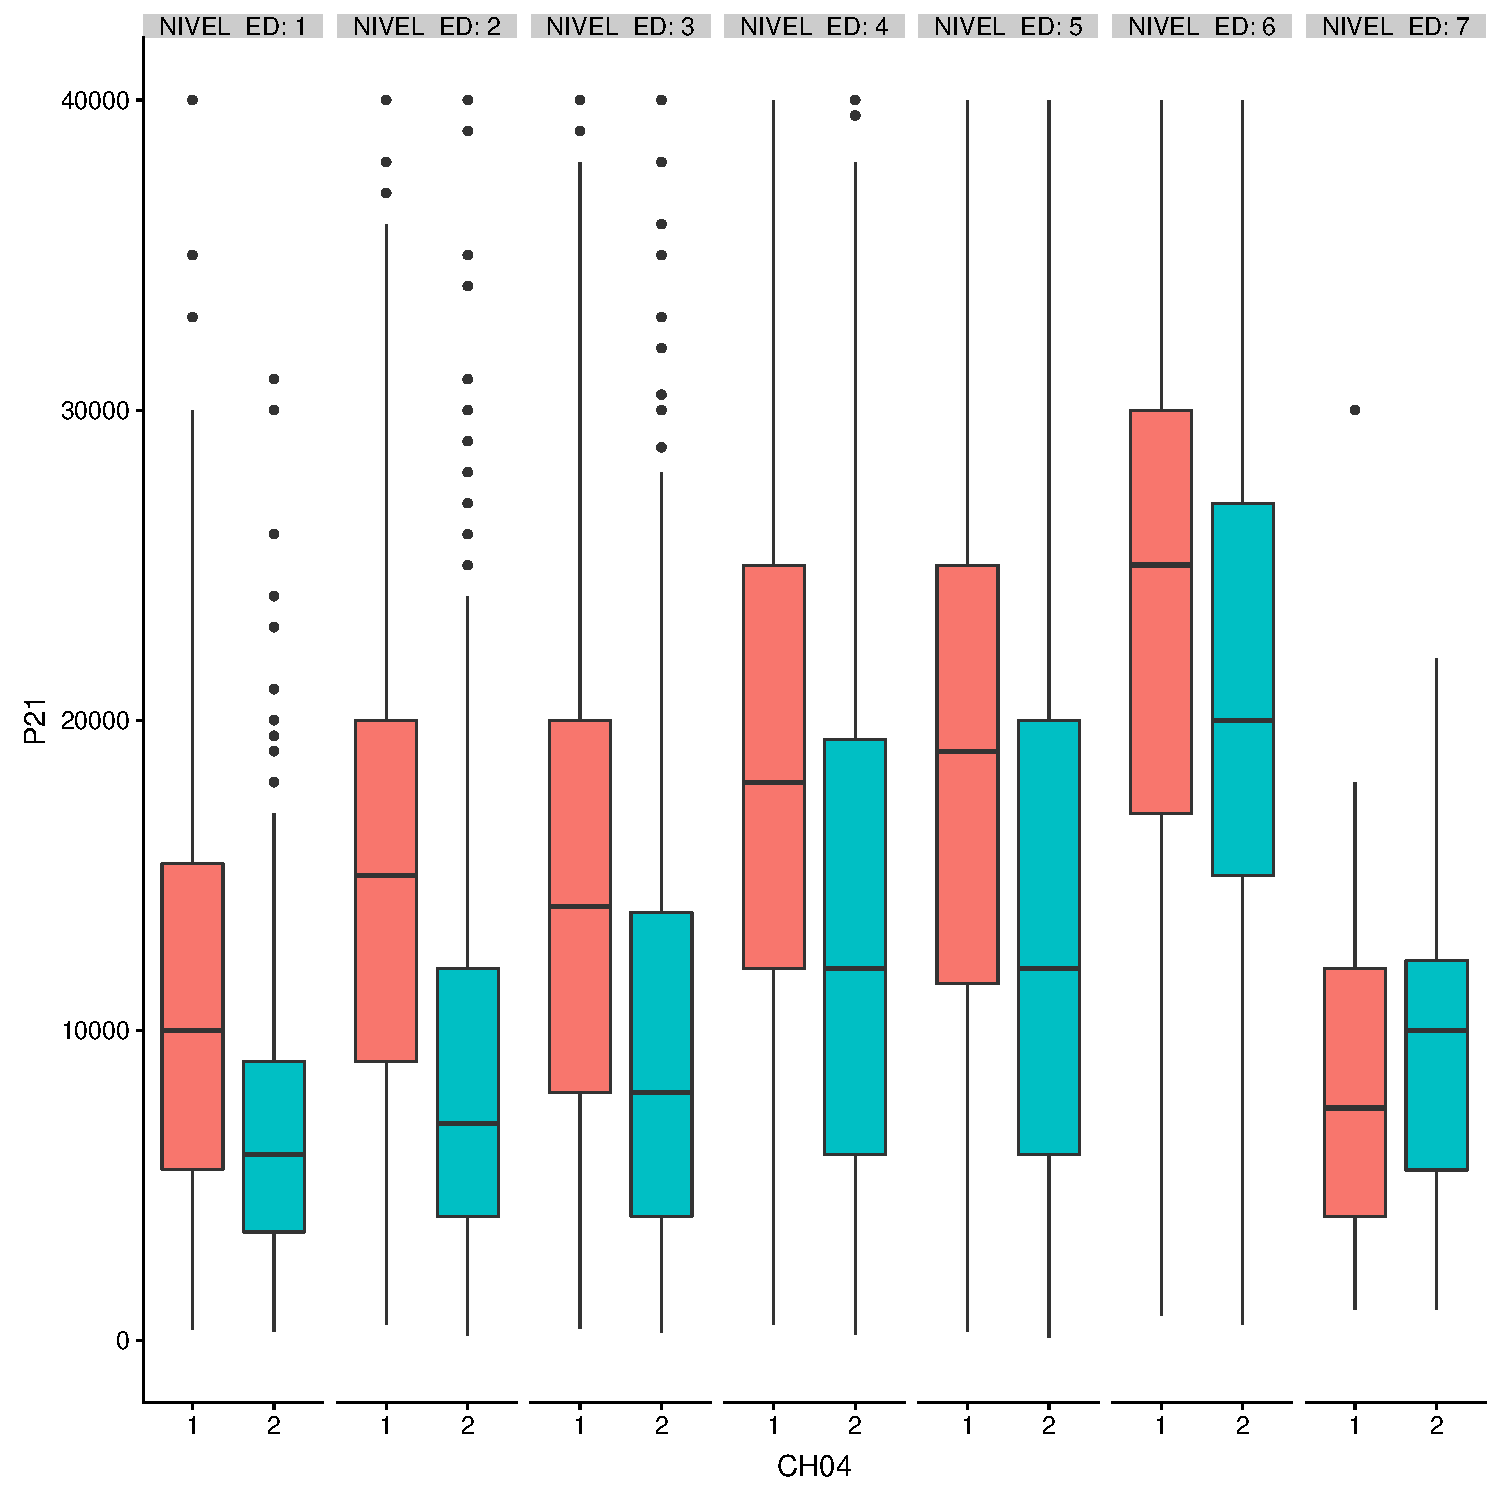
\includegraphics{bookdown_files/figure-latex/unnamed-chunk-93-1.pdf}

\hypertarget{histogramas}{%
\subsection{\texorpdfstring{\href{https://ggplot2.tidyverse.org/reference/geom_histogram.html}{Histogramas}}{Histogramas}}\label{histogramas}}

Por ejemplo, si observamos el ingreso de la ocupación principal:

\begin{Shaded}
\begin{Highlighting}[]
\NormalTok{hist_data <-Individual_t119 }\OperatorTok
\StringTok{  }\KeywordTok{filter}\NormalTok{(P21}\OperatorTok{>}\DecValTok{0}\NormalTok{) }

\KeywordTok{ggplot}\NormalTok{(hist_data, }\KeywordTok{aes}\NormalTok{(}\DataTypeTok{x =}\NormalTok{ P21,}\DataTypeTok{weights =}\NormalTok{ PONDIIO))}\OperatorTok{+}\StringTok{ }
\KeywordTok{geom_histogram}\NormalTok{()}\OperatorTok{+}
\KeywordTok{scale_x_continuous}\NormalTok{(}\DataTypeTok{limits =} \KeywordTok{c}\NormalTok{(}\DecValTok{0}\NormalTok{,}\DecValTok{50000}\NormalTok{))}
\end{Highlighting}
\end{Shaded}

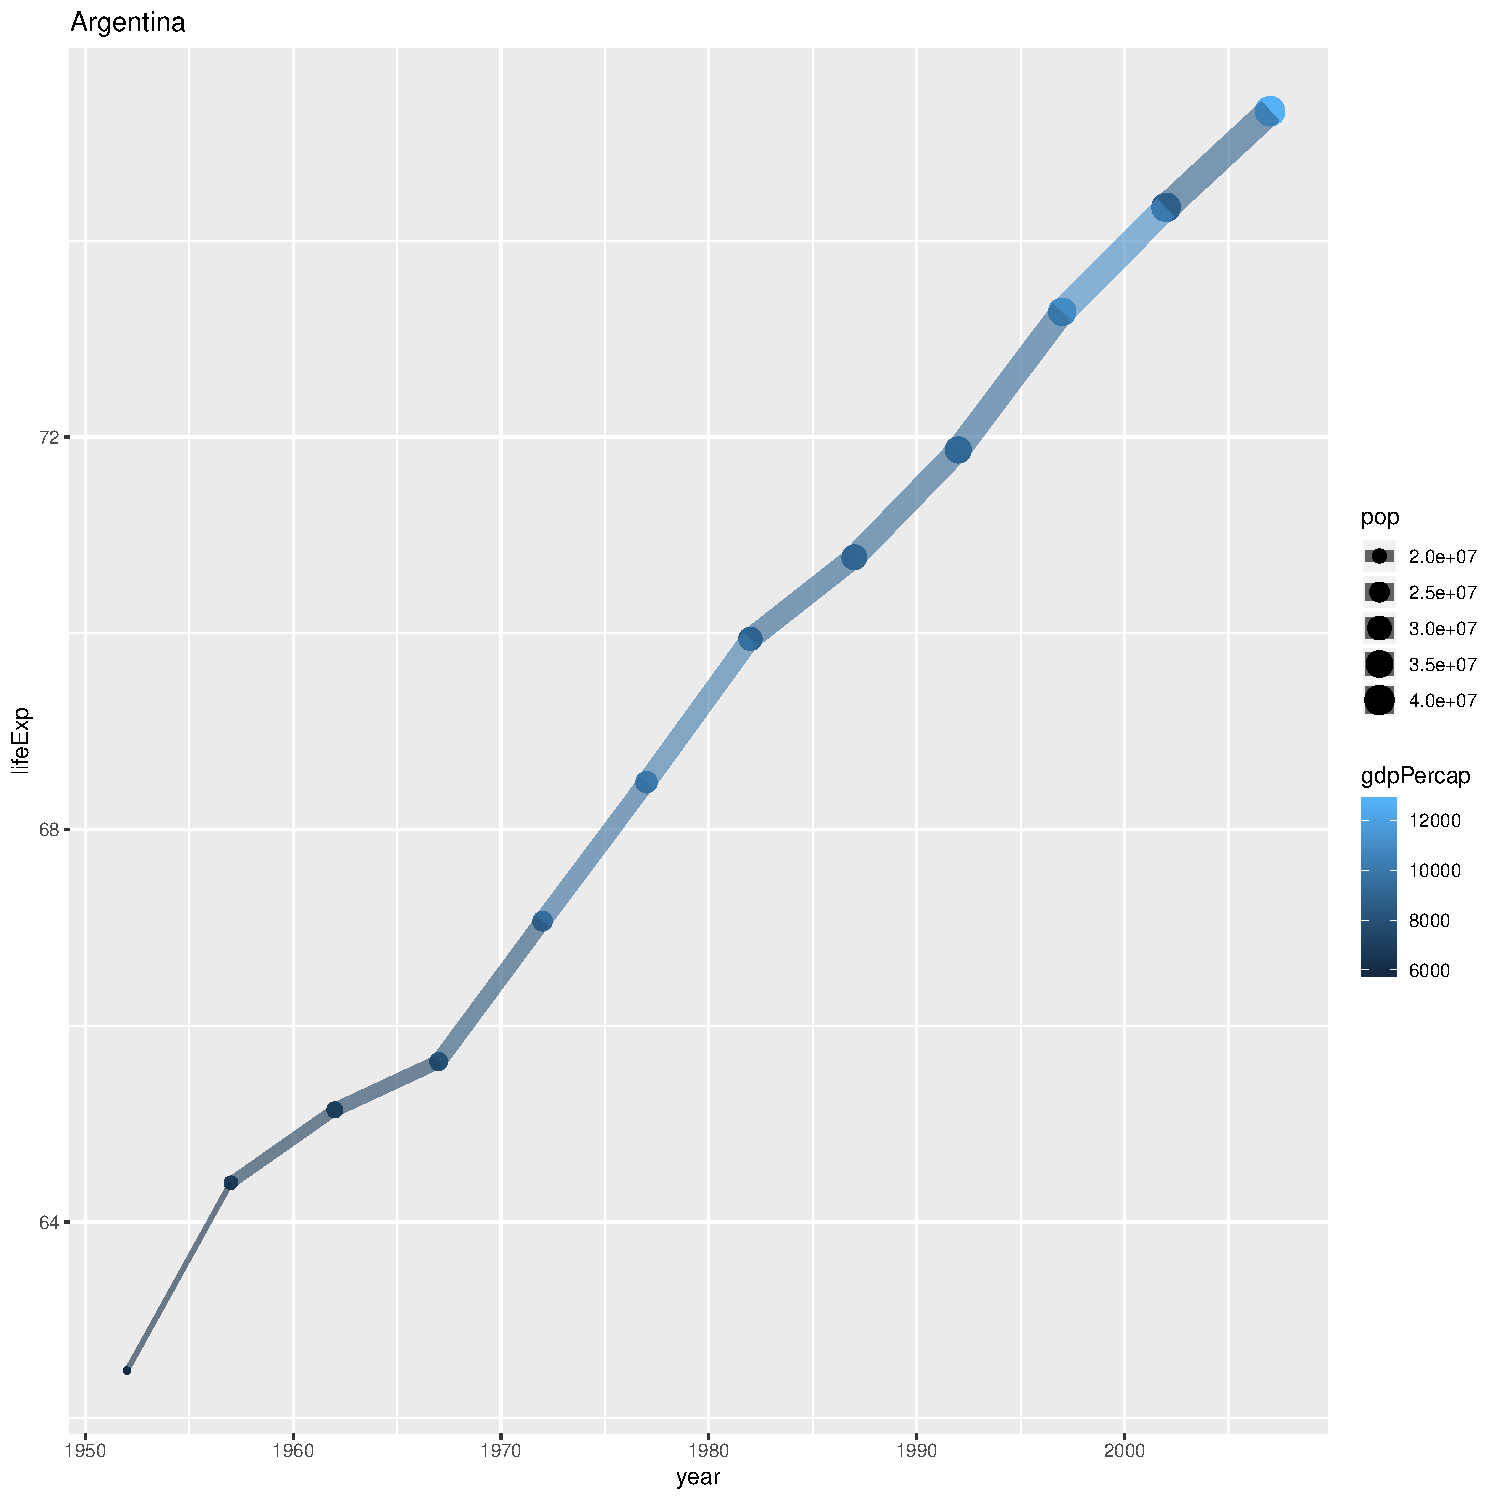
\includegraphics{bookdown_files/figure-latex/unnamed-chunk-94-1.pdf}

En este gráfico, los posibles valores de p21 se dividen en 30 \textbf{bins} consecutivos y el gráfico muestra cuantas observaciones caen en cada uno de ellos

\hypertarget{kernels}{%
\subsection{\texorpdfstring{\href{https://plot.ly/ggplot2/geom_density/}{Kernels}}{Kernels}}\label{kernels}}

La función \texttt{geom\_density()} nos permite construir \textbf{kernels} de la distribución. Es particularmente útil cuando tenemos una variable continua, dado que los histogramas rompen esa sensación de continuidad.

Veamos un ejemplo sencillo con los ingresos de la ocupación principal. Luego iremos complejizandolo

\begin{Shaded}
\begin{Highlighting}[]
\NormalTok{kernel_data <-Individual_t119 }\OperatorTok
\StringTok{  }\KeywordTok{filter}\NormalTok{(P21}\OperatorTok{>}\DecValTok{0}\NormalTok{) }

\KeywordTok{ggplot}\NormalTok{(kernel_data, }\KeywordTok{aes}\NormalTok{(}\DataTypeTok{x =}\NormalTok{ P21,}\DataTypeTok{weights =}\NormalTok{ PONDIIO))}\OperatorTok{+}\StringTok{ }
\KeywordTok{geom_density}\NormalTok{()}\OperatorTok{+}
\KeywordTok{scale_x_continuous}\NormalTok{(}\DataTypeTok{limits =} \KeywordTok{c}\NormalTok{(}\DecValTok{0}\NormalTok{,}\DecValTok{50000}\NormalTok{))}
\end{Highlighting}
\end{Shaded}

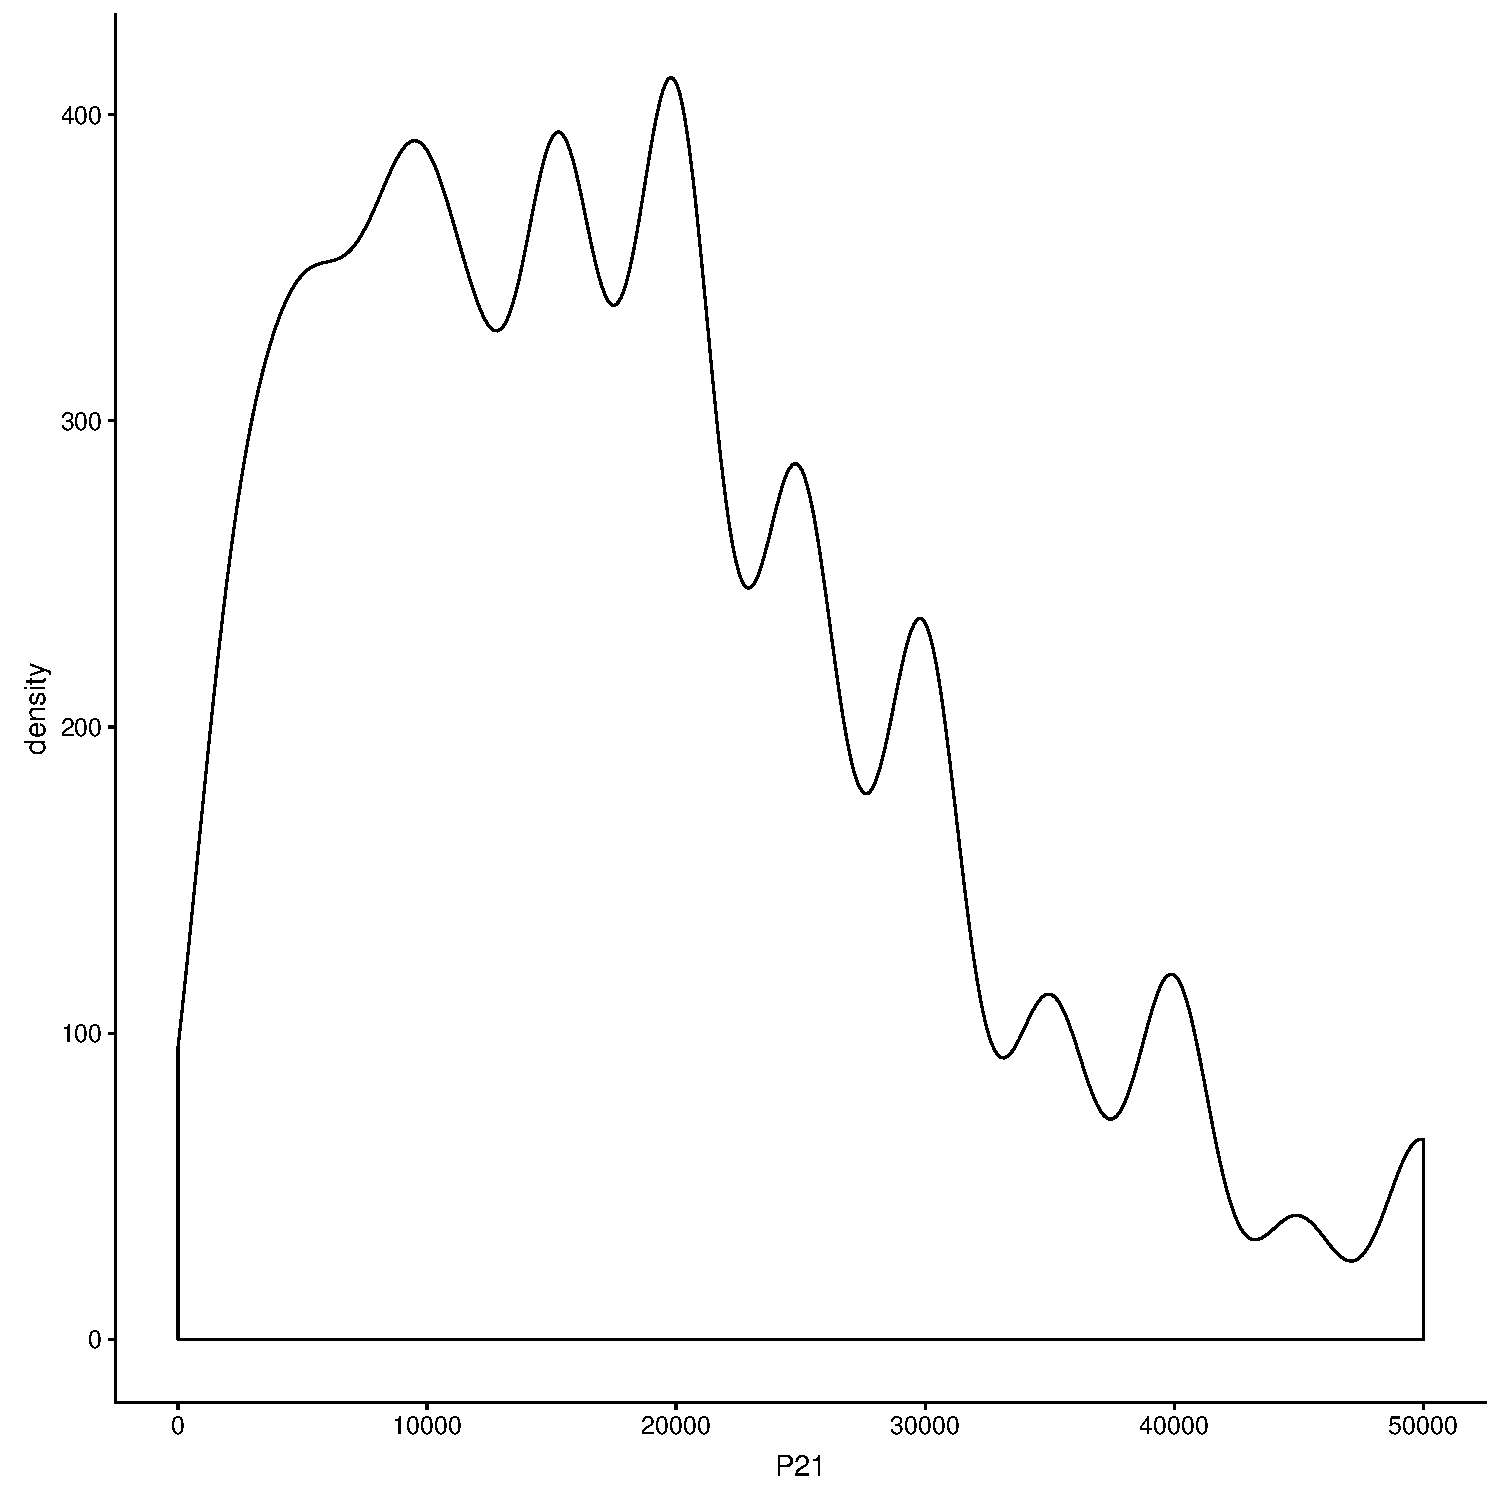
\includegraphics{bookdown_files/figure-latex/unnamed-chunk-95-1.pdf}
\textbf{El eje y no tiene demasiada interpretabilidad en los Kernel, porque hace a la forma en que se construyen las distribuciones}.

El parametro adjust, dentro de la función \texttt{geom\_density}nos permite reducir o ampliar el rango de suavizado de la distribución. Su valor por default es 1. Veamos que sucede si lo seteamos en 2

\begin{Shaded}
\begin{Highlighting}[]
\KeywordTok{ggplot}\NormalTok{(kernel_data, }\KeywordTok{aes}\NormalTok{(}\DataTypeTok{x =}\NormalTok{ P21,}\DataTypeTok{weights =}\NormalTok{ PONDIIO))}\OperatorTok{+}\StringTok{ }
\KeywordTok{geom_density}\NormalTok{(}\DataTypeTok{adjust =} \DecValTok{2}\NormalTok{)}\OperatorTok{+}
\KeywordTok{scale_x_continuous}\NormalTok{(}\DataTypeTok{limits =} \KeywordTok{c}\NormalTok{(}\DecValTok{0}\NormalTok{,}\DecValTok{50000}\NormalTok{))}
\end{Highlighting}
\end{Shaded}

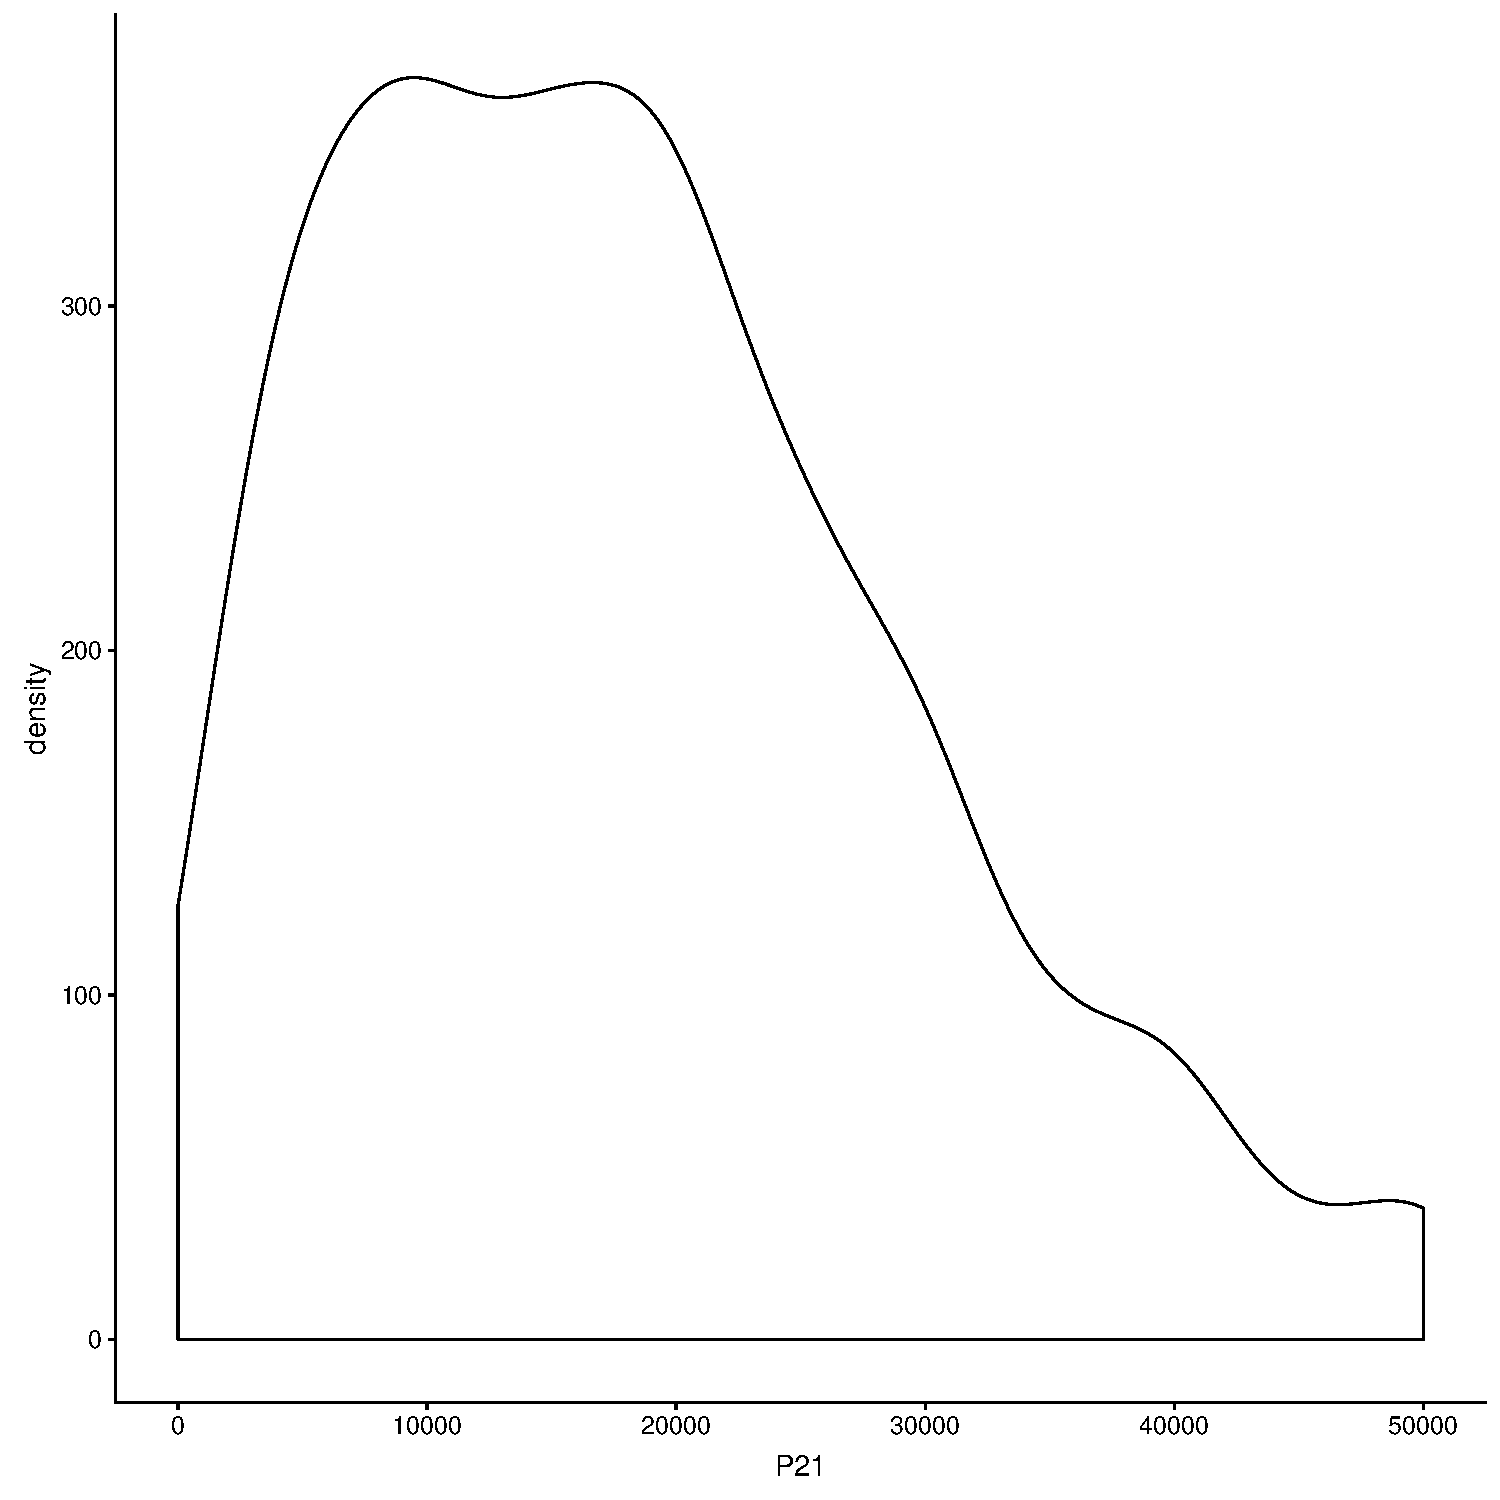
\includegraphics{bookdown_files/figure-latex/unnamed-chunk-96-1.pdf}

Como es esperable, la distribución del ingreso tiene ``picos'' en los valores redondos, ya que la gente suele declarar un valor aproximado al ingreso efectivo que percibe. Nadie declara ingresos de 30001. Al suavizar la serie con un kernel, eliminamos ese efecto.Si seteamos el rango para el suavizado en valores menores a 1, podemos observar estos picos.

\begin{Shaded}
\begin{Highlighting}[]
\KeywordTok{ggplot}\NormalTok{(kernel_data, }\KeywordTok{aes}\NormalTok{(}\DataTypeTok{x =}\NormalTok{ P21,}\DataTypeTok{weights =}\NormalTok{ PONDIIO))}\OperatorTok{+}\StringTok{ }
\KeywordTok{geom_density}\NormalTok{(}\DataTypeTok{adjust =} \FloatTok{0.01}\NormalTok{)}\OperatorTok{+}
\KeywordTok{scale_x_continuous}\NormalTok{(}\DataTypeTok{limits =} \KeywordTok{c}\NormalTok{(}\DecValTok{0}\NormalTok{,}\DecValTok{50000}\NormalTok{))}
\end{Highlighting}
\end{Shaded}

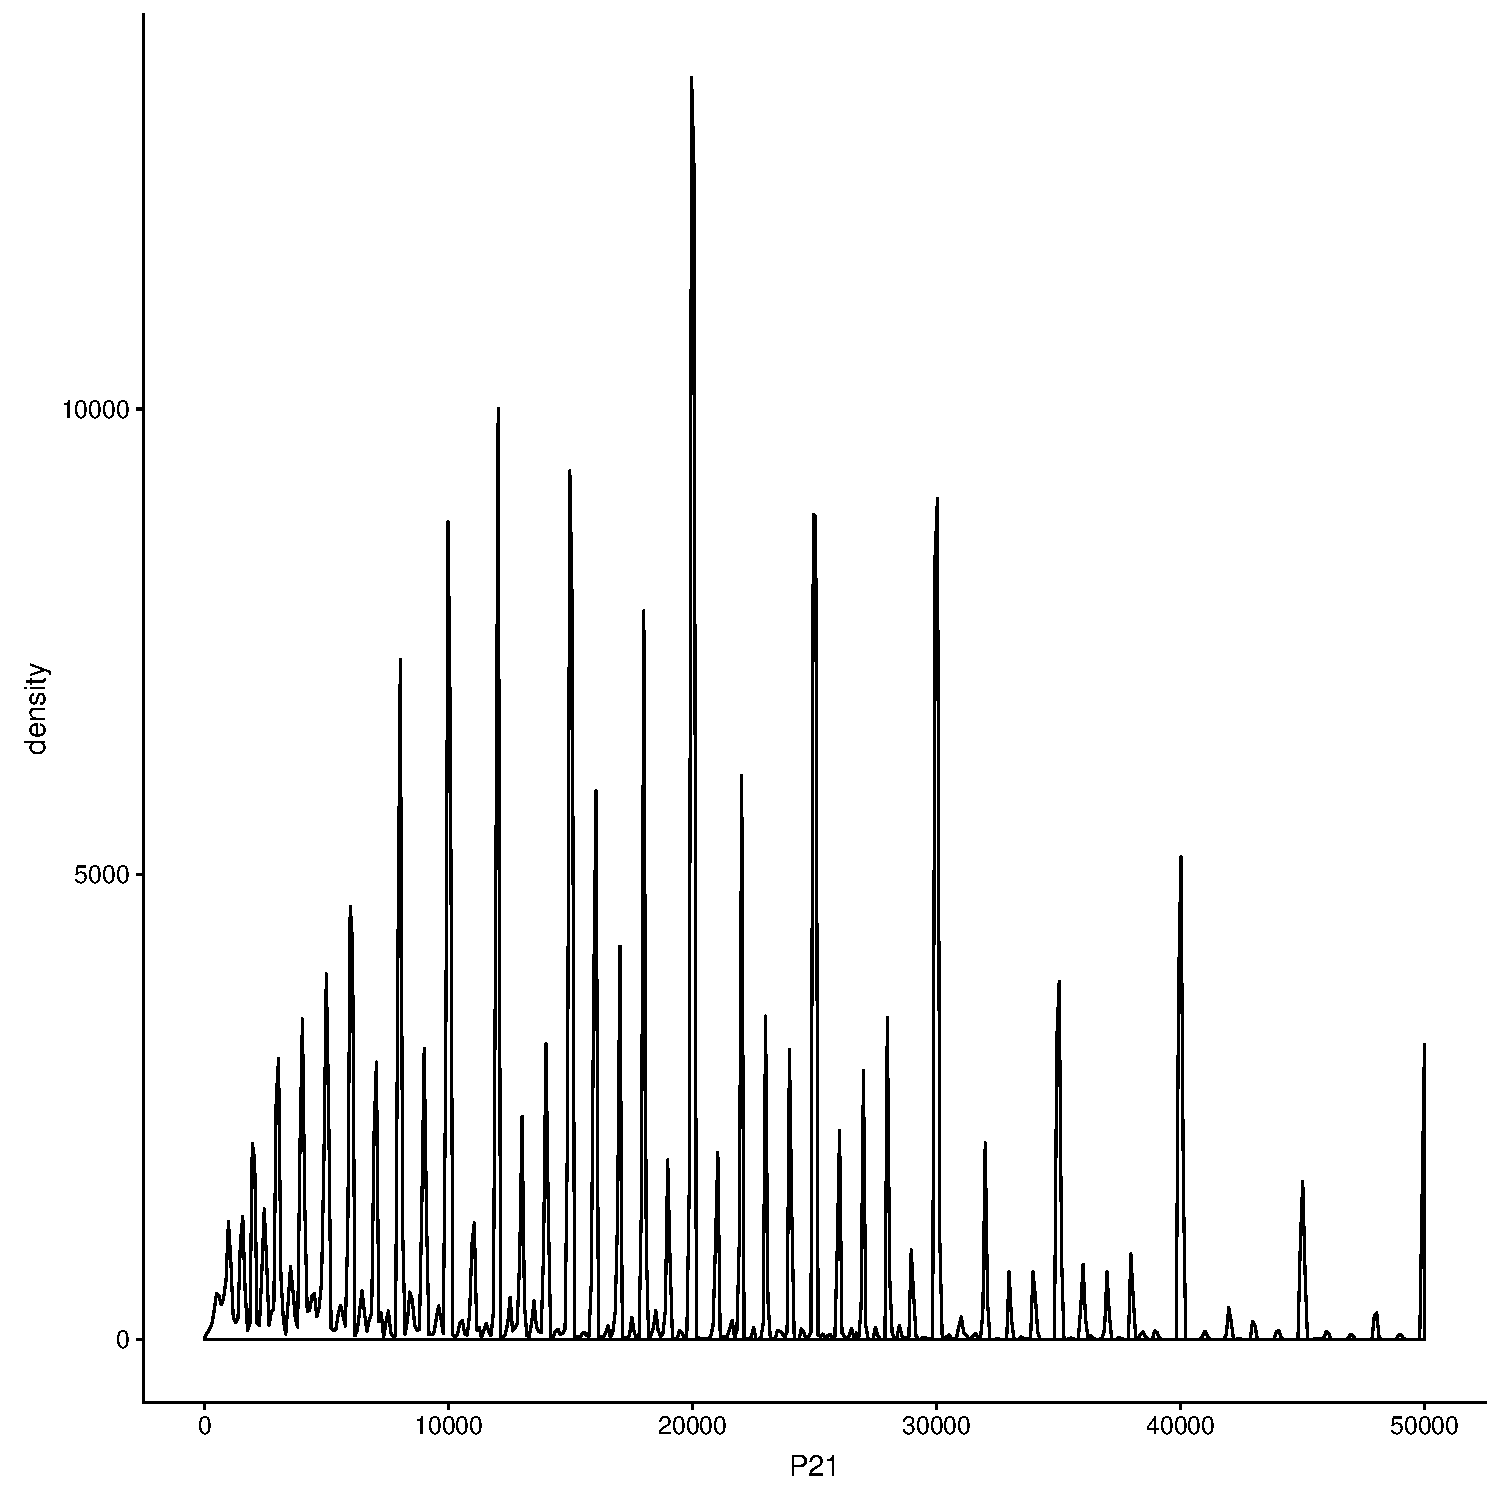
\includegraphics{bookdown_files/figure-latex/unnamed-chunk-97-1.pdf}

Ahora bien, como en todo grafico de R, podemos seguir agregando dimensiones para enriquecer el análisis.

\begin{Shaded}
\begin{Highlighting}[]
\NormalTok{kernel_data_}\DecValTok{2}\NormalTok{ <-}\StringTok{ }\NormalTok{kernel_data }\OperatorTok\StringTok{ }
\StringTok{  }\KeywordTok{mutate}\NormalTok{(}\DataTypeTok{CH04=} \KeywordTok{case_when}\NormalTok{(CH04 }\OperatorTok{==}\StringTok{ }\DecValTok{1} \OperatorTok{~}\StringTok{ "Varon"}\NormalTok{,}
\NormalTok{                         CH04 }\OperatorTok{==}\StringTok{ }\DecValTok{2} \OperatorTok{~}\StringTok{ "Mujer"}\NormalTok{))}
  
\KeywordTok{ggplot}\NormalTok{(kernel_data_}\DecValTok{2}\NormalTok{, }\KeywordTok{aes}\NormalTok{(}\DataTypeTok{x =}\NormalTok{ P21,}
  \DataTypeTok{weights =}\NormalTok{ PONDIIO,}
  \DataTypeTok{group =}\NormalTok{ CH04,}
  \DataTypeTok{fill =}\NormalTok{ CH04)) }\OperatorTok{+}
\StringTok{  }\KeywordTok{geom_density}\NormalTok{(}\DataTypeTok{alpha=}\FloatTok{0.7}\NormalTok{,}\DataTypeTok{adjust =}\DecValTok{2}\NormalTok{)}\OperatorTok{+}
\StringTok{  }\KeywordTok{labs}\NormalTok{(}\DataTypeTok{x=}\StringTok{"Distribución del ingreso"}\NormalTok{, }\DataTypeTok{y=}\StringTok{""}\NormalTok{,}
       \DataTypeTok{title=}\StringTok{" Total según tipo de ingreso y sexo"}\NormalTok{, }
       \DataTypeTok{caption =} \StringTok{"Fuente: Encuesta Permanente de Hogares"}\NormalTok{)}\OperatorTok{+}
\StringTok{  }\KeywordTok{scale_x_continuous}\NormalTok{(}\DataTypeTok{limits =} \KeywordTok{c}\NormalTok{(}\DecValTok{0}\NormalTok{,}\DecValTok{50000}\NormalTok{))}\OperatorTok{+}
\StringTok{  }\KeywordTok{theme_tufte}\NormalTok{()}\OperatorTok{+}
\StringTok{  }\KeywordTok{scale_fill_gdocs}\NormalTok{()}\OperatorTok{+}
\StringTok{  }\KeywordTok{theme}\NormalTok{(}\DataTypeTok{legend.position =} \StringTok{"bottom"}\NormalTok{,}
        \DataTypeTok{plot.title      =} \KeywordTok{element_text}\NormalTok{(}\DataTypeTok{size=}\DecValTok{12}\NormalTok{))}
\end{Highlighting}
\end{Shaded}

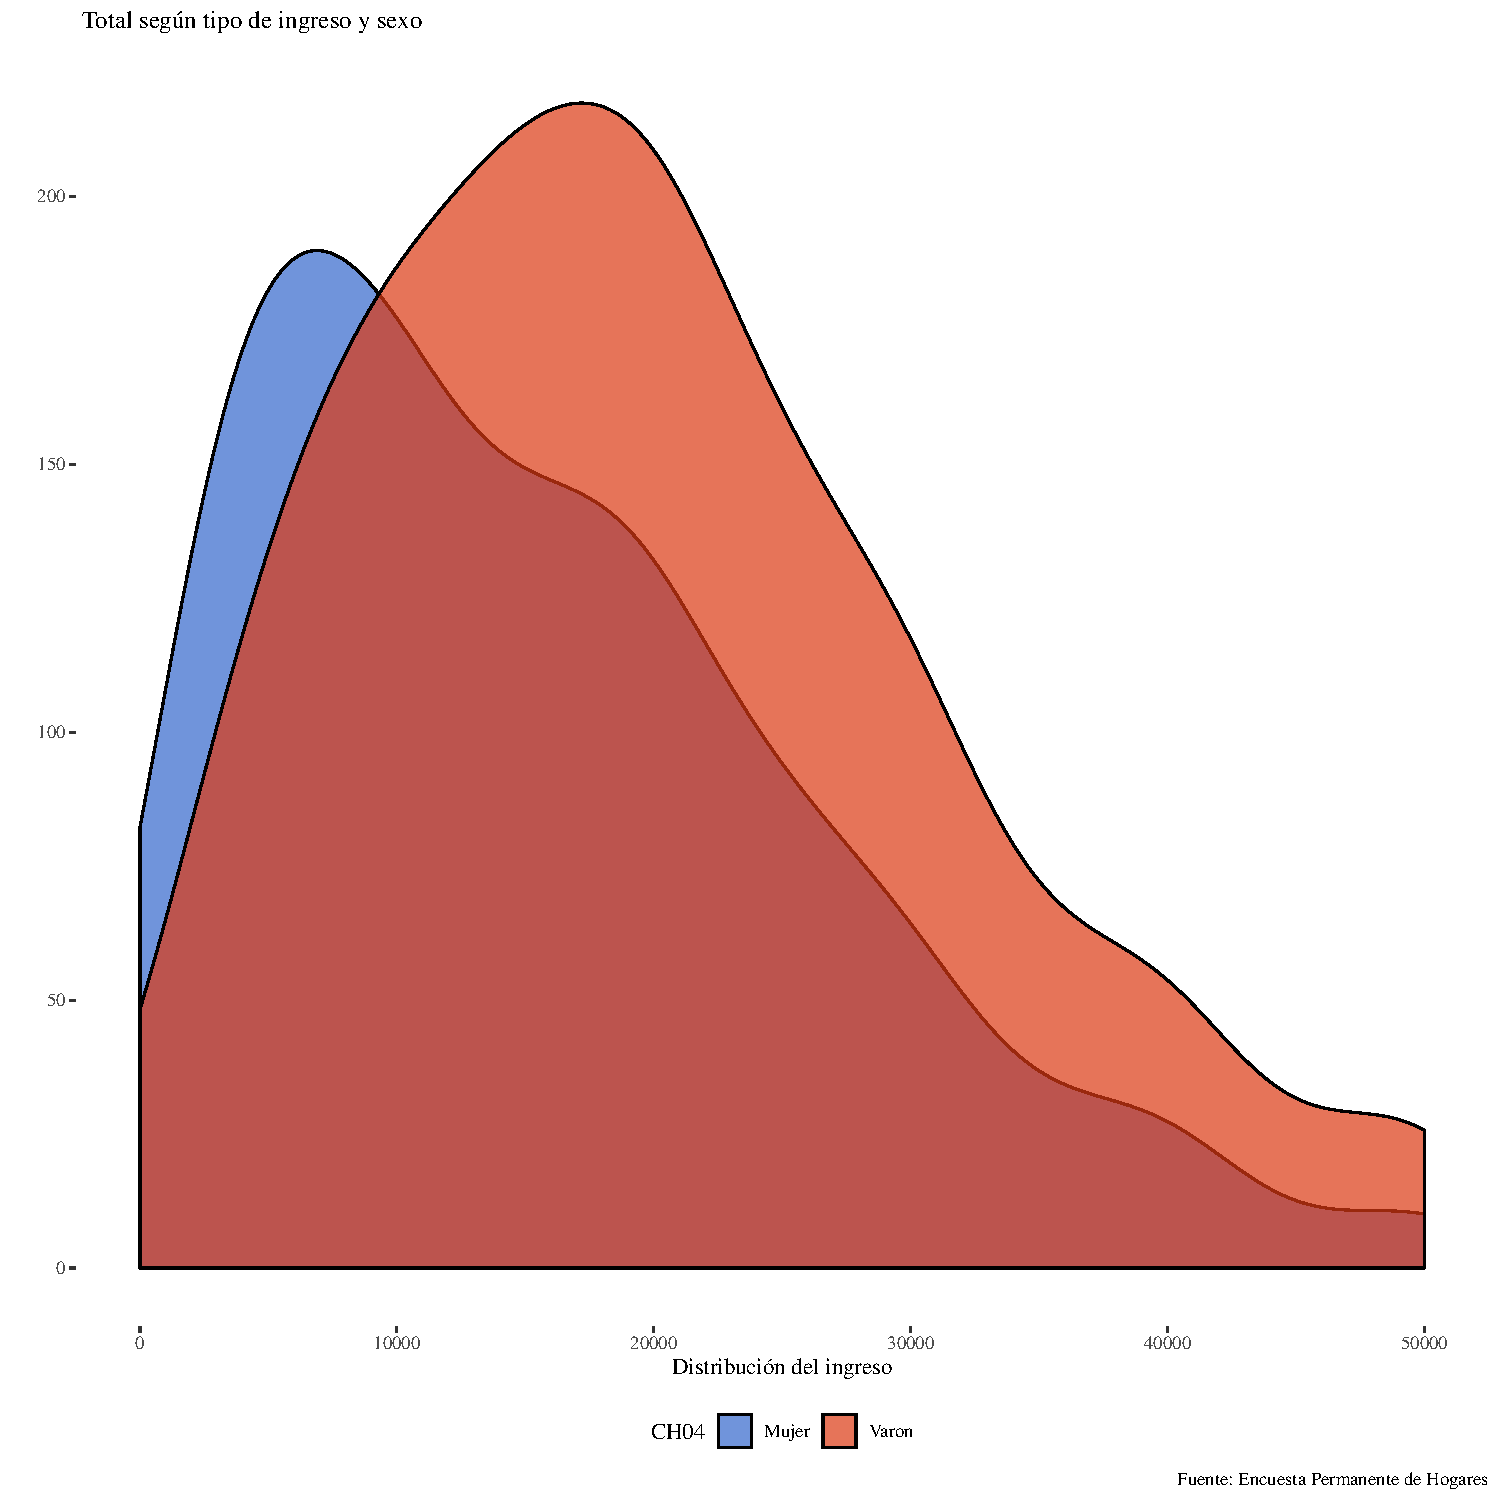
\includegraphics{bookdown_files/figure-latex/unnamed-chunk-98-1.pdf}

\begin{Shaded}
\begin{Highlighting}[]
\KeywordTok{ggsave}\NormalTok{(}\DataTypeTok{filename =} \StringTok{"resultados/Kernel_1.png"}\NormalTok{,}\DataTypeTok{scale =} \DecValTok{2}\NormalTok{)}
\end{Highlighting}
\end{Shaded}

Podemos agregar aún la dimensión de ingreso laboral respecto del no laboral

\begin{Shaded}
\begin{Highlighting}[]
\NormalTok{kernel_data_}\DecValTok{3}\NormalTok{ <-kernel_data_}\DecValTok{2} \OperatorTok\StringTok{ }
\StringTok{  }\KeywordTok{select}\NormalTok{(REGION,P47T,T_VI, TOT_P12, P21 , PONDII, CH04) }\OperatorTok\StringTok{ }
\StringTok{  }\KeywordTok{filter}\NormalTok{(}\OperatorTok{!}\KeywordTok{is.na}\NormalTok{(P47T), P47T }\OperatorTok{>}\StringTok{ }\DecValTok{0}\NormalTok{ ) }\OperatorTok\StringTok{ }
\StringTok{  }\KeywordTok{mutate}\NormalTok{(}\DataTypeTok{ingreso_laboral    =}\NormalTok{ TOT_P12 }\OperatorTok{+}\StringTok{ }\NormalTok{P21,}
         \DataTypeTok{ingreso_no_laboral =}\NormalTok{ T_VI) }\OperatorTok
\StringTok{  }\KeywordTok{gather}\NormalTok{(., }\DataTypeTok{key =}\NormalTok{ Tipo_ingreso, Ingreso, }\KeywordTok{c}\NormalTok{((}\KeywordTok{ncol}\NormalTok{(.)}\OperatorTok{-}\DecValTok{1}\NormalTok{)}\OperatorTok{:}\KeywordTok{ncol}\NormalTok{(.))) }\OperatorTok
\StringTok{  }\KeywordTok{filter}\NormalTok{( Ingreso }\OperatorTok{!=}\DecValTok{0}\NormalTok{)}\CommentTok{# Para este gráfico, quiero eliminar los ingresos = 0}

\NormalTok{kernel_data_}\DecValTok{3} \OperatorTok\StringTok{ }
\StringTok{  }\KeywordTok{sample_n}\NormalTok{(}\DecValTok{10}\NormalTok{)}
\end{Highlighting}
\end{Shaded}

\begin{verbatim}
##    REGION  P47T  T_VI TOT_P12   P21 PONDII  CH04       Tipo_ingreso
## 1      44 30000     0       0 20000    154 Mujer    ingreso_laboral
## 2      44 40000  1000       0 39000     39 Mujer    ingreso_laboral
## 3      40 31000 28000       0  3000    231 Mujer    ingreso_laboral
## 4      41 16500  2500       0 14000     44 Mujer    ingreso_laboral
## 5      40 34000     0       0 23000    158 Mujer    ingreso_laboral
## 6       1  3000  1000       0  2000   2751 Mujer ingreso_no_laboral
## 7      43 65000     0       0 65000    682 Mujer    ingreso_laboral
## 8      41 10000     0       0 10000    325 Varon    ingreso_laboral
## 9      44 18000     0       0 18000    181 Varon    ingreso_laboral
## 10     43 50000     0   20000 30000    362 Varon    ingreso_laboral
##    Ingreso
## 1    20000
## 2    39000
## 3     3000
## 4    14000
## 5    23000
## 6     1000
## 7    65000
## 8    10000
## 9    18000
## 10   50000
\end{verbatim}

\begin{Shaded}
\begin{Highlighting}[]
  \KeywordTok{ggplot}\NormalTok{(kernel_data_}\DecValTok{3}\NormalTok{, }\KeywordTok{aes}\NormalTok{(}
  \DataTypeTok{x =}\NormalTok{ Ingreso,}
  \DataTypeTok{weights =}\NormalTok{ PONDII,}
  \DataTypeTok{group =}\NormalTok{ Tipo_ingreso,}
  \DataTypeTok{fill =}\NormalTok{ Tipo_ingreso)) }\OperatorTok{+}
\StringTok{  }\KeywordTok{geom_density}\NormalTok{(}\DataTypeTok{alpha=}\FloatTok{0.7}\NormalTok{,}\DataTypeTok{adjust =}\DecValTok{2}\NormalTok{)}\OperatorTok{+}
\StringTok{  }\KeywordTok{labs}\NormalTok{(}\DataTypeTok{x=}\StringTok{"Distribución del ingreso"}\NormalTok{, }\DataTypeTok{y=}\StringTok{""}\NormalTok{,}
       \DataTypeTok{title=}\StringTok{" Total según tipo de ingreso y sexo"}\NormalTok{, }
       \DataTypeTok{caption =} \StringTok{"Fuente: Encuesta Permanente de Hogares"}\NormalTok{)}\OperatorTok{+}
\StringTok{  }\KeywordTok{scale_x_continuous}\NormalTok{(}\DataTypeTok{limits =} \KeywordTok{c}\NormalTok{(}\DecValTok{0}\NormalTok{,}\DecValTok{50000}\NormalTok{))}\OperatorTok{+}
\StringTok{  }\KeywordTok{theme_tufte}\NormalTok{()}\OperatorTok{+}
\StringTok{  }\KeywordTok{scale_fill_gdocs}\NormalTok{()}\OperatorTok{+}
\StringTok{  }\KeywordTok{theme}\NormalTok{(}\DataTypeTok{legend.position =} \StringTok{"bottom"}\NormalTok{,}
        \DataTypeTok{plot.title      =} \KeywordTok{element_text}\NormalTok{(}\DataTypeTok{size=}\DecValTok{12}\NormalTok{))}\OperatorTok{+}
\StringTok{  }\KeywordTok{facet_wrap}\NormalTok{(}\OperatorTok{~}\StringTok{ }\NormalTok{CH04, }\DataTypeTok{scales =} \StringTok{"free"}\NormalTok{)}
\end{Highlighting}
\end{Shaded}

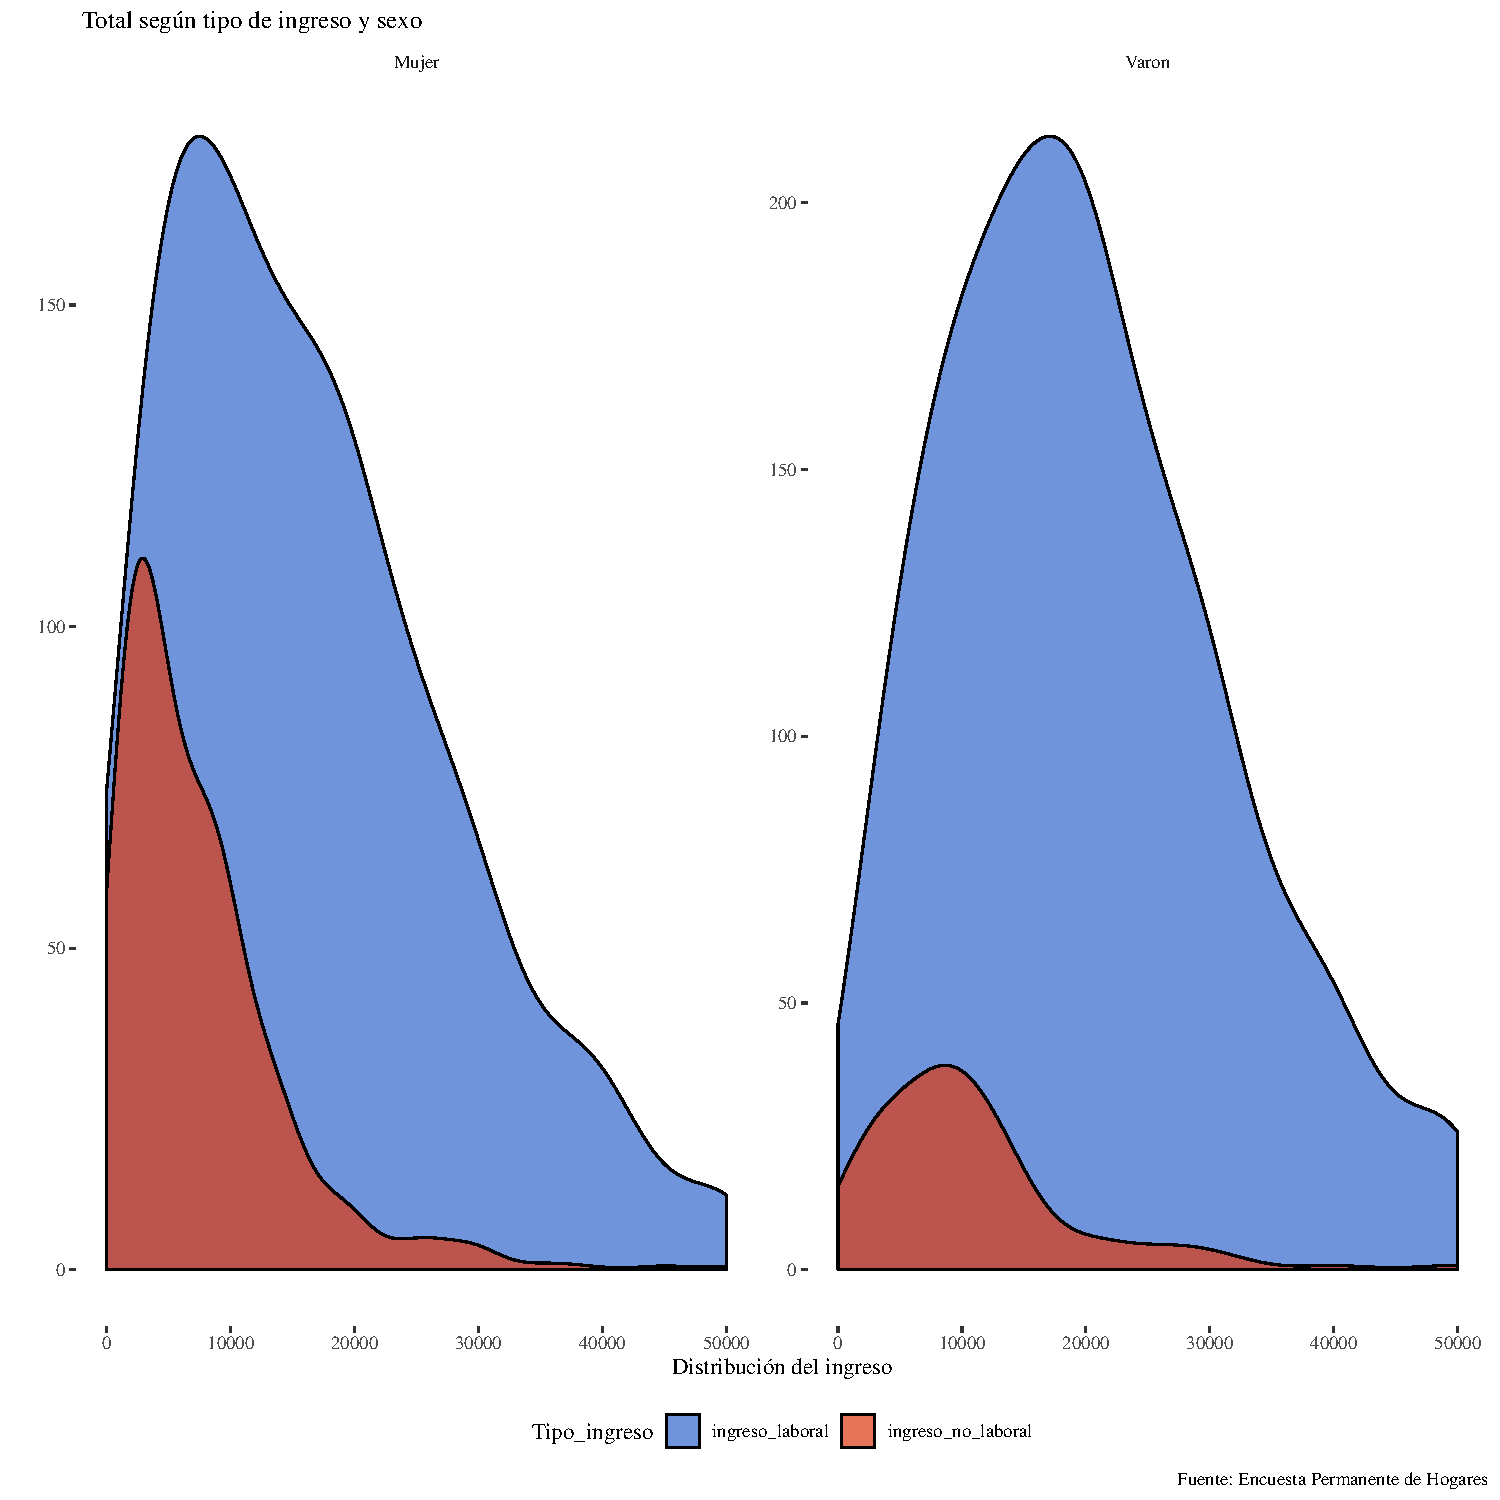
\includegraphics{bookdown_files/figure-latex/unnamed-chunk-100-1.pdf}

\begin{Shaded}
\begin{Highlighting}[]
\KeywordTok{ggsave}\NormalTok{(}\DataTypeTok{filename =} \StringTok{"resultados/Kernel_2.png"}\NormalTok{,}\DataTypeTok{scale =} \DecValTok{2}\NormalTok{)}
\end{Highlighting}
\end{Shaded}

En este tipo de gráficos, importa mucho qué variable se utiliza para \emph{facetear} y qué variable para agrupar, ya que la construcción de la distribución es diferente.

\begin{Shaded}
\begin{Highlighting}[]
\KeywordTok{ggplot}\NormalTok{(kernel_data_}\DecValTok{3}\NormalTok{, }\KeywordTok{aes}\NormalTok{(}
  \DataTypeTok{x =}\NormalTok{ Ingreso,}
  \DataTypeTok{weights =}\NormalTok{ PONDII,}
  \DataTypeTok{group =}\NormalTok{ CH04,}
  \DataTypeTok{fill =}\NormalTok{ CH04)) }\OperatorTok{+}
\StringTok{  }\KeywordTok{geom_density}\NormalTok{(}\DataTypeTok{alpha=}\FloatTok{0.7}\NormalTok{,}\DataTypeTok{adjust =}\DecValTok{2}\NormalTok{)}\OperatorTok{+}
\StringTok{  }\KeywordTok{labs}\NormalTok{(}\DataTypeTok{x=}\StringTok{"Distribución del ingreso"}\NormalTok{, }\DataTypeTok{y=}\StringTok{""}\NormalTok{,}
       \DataTypeTok{title=}\StringTok{" Total según tipo de ingreso y sexo"}\NormalTok{, }
       \DataTypeTok{caption =} \StringTok{"Fuente: Encuesta Permanente de Hogares"}\NormalTok{)}\OperatorTok{+}
\StringTok{  }\KeywordTok{scale_x_continuous}\NormalTok{(}\DataTypeTok{limits =} \KeywordTok{c}\NormalTok{(}\DecValTok{0}\NormalTok{,}\DecValTok{50000}\NormalTok{))}\OperatorTok{+}
\StringTok{  }\KeywordTok{theme_tufte}\NormalTok{()}\OperatorTok{+}
\StringTok{  }\KeywordTok{scale_fill_gdocs}\NormalTok{()}\OperatorTok{+}
\StringTok{  }\KeywordTok{theme}\NormalTok{(}\DataTypeTok{legend.position =} \StringTok{"bottom"}\NormalTok{,}
        \DataTypeTok{plot.title      =} \KeywordTok{element_text}\NormalTok{(}\DataTypeTok{size=}\DecValTok{12}\NormalTok{))}\OperatorTok{+}
\StringTok{  }\KeywordTok{facet_wrap}\NormalTok{(}\OperatorTok{~}\NormalTok{Tipo_ingreso, }\DataTypeTok{scales =} \StringTok{"free"}\NormalTok{)}
\end{Highlighting}
\end{Shaded}

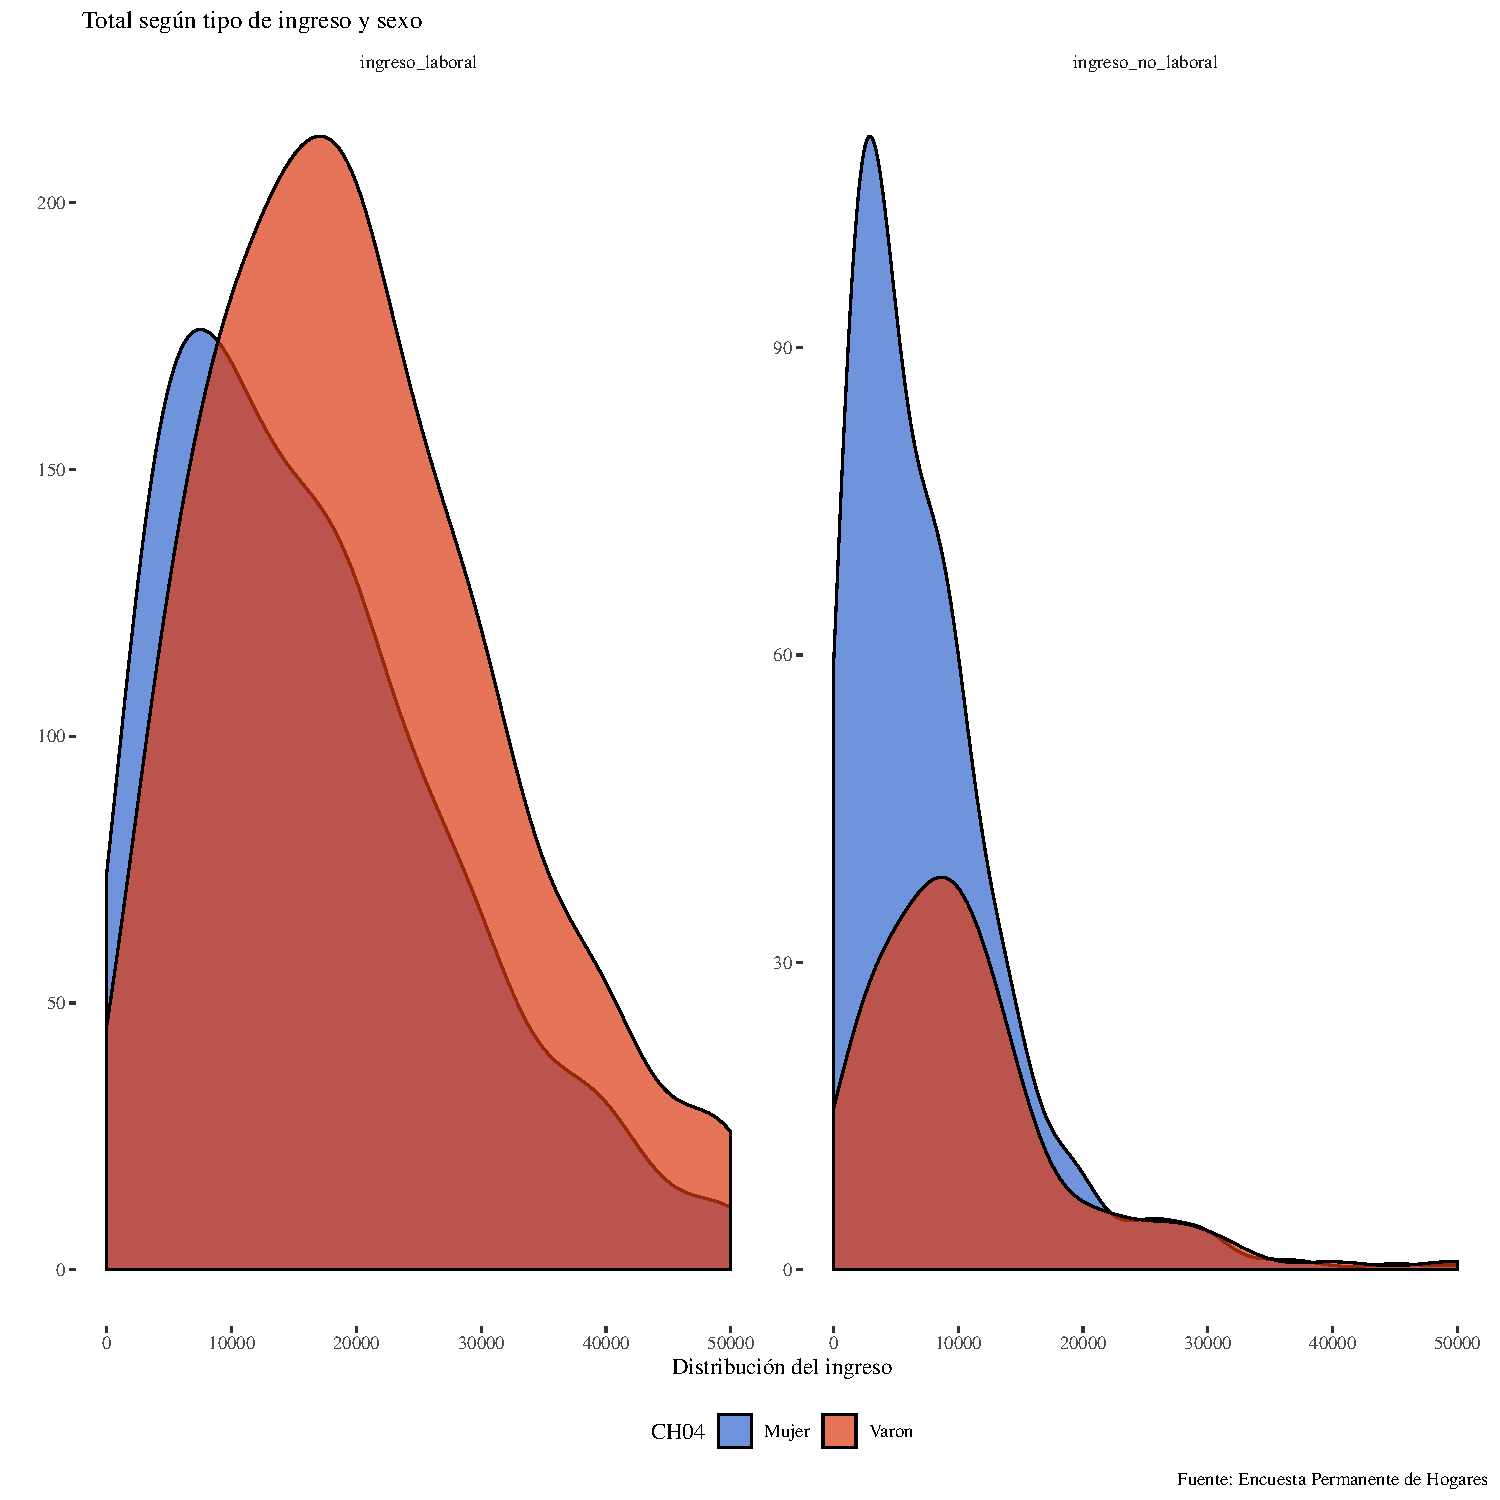
\includegraphics{bookdown_files/figure-latex/unnamed-chunk-101-1.pdf}

\begin{Shaded}
\begin{Highlighting}[]
\KeywordTok{ggsave}\NormalTok{(}\DataTypeTok{filename =} \StringTok{"resultados/Kernel_3.png"}\NormalTok{,}\DataTypeTok{scale =} \DecValTok{2}\NormalTok{)}
\end{Highlighting}
\end{Shaded}

\hypertarget{documentacion}{%
\chapter{Documentación}\label{documentacion}}

\begin{itemize}
\tightlist
\item
  Manejo de las extensiones del software ``Rmarkdown'' y ``RNotebook'' para elaborar documentos de trabajo, presentaciones interactivas e informes:
\item
  Opciones para mostrar u ocultar código en los reportes
\item
  Definición de tamaño, títulos y formato con el cual se despliegan los gráficos y tablas en el informe
\item
  Caracteres especiales para incluir múltiples recursos en el texto del informe: Links a páginas web, notas al pie, enumeraciones, cambios en el formato de letra (tamaño, negrita, cursiva)
\item
  Código embebido en el texto para automatización de reportes
\end{itemize}

\hypertarget{explicacion-3}{%
\section{Explicación}\label{explicacion-3}}

\hypertarget{practica-guiada-3}{%
\section{Práctica Guiada}\label{practica-guiada-3}}

\hypertarget{probabilidad-y-estadistica}{%
\chapter{Probabilidad y Estadística}\label{probabilidad-y-estadistica}}

Esta clase es un repaso de los rudimentos de probabilidad y estadística. El objetivo es obtener las herramientas básicas para la interpretación de resultados estadísticos.

\begin{itemize}
\tightlist
\item
  Introducción a probabilidad
\item
  Introducción a distribuciones
\item
  El problema de la inversión
\item
  Estadística
\item
  Población y muestra
\item
  Estimadores puntuales, tests de hipótesis
\item
  Boxplots, histogramas y kernels
\end{itemize}

\hypertarget{explicacion-4}{%
\section{Explicación}\label{explicacion-4}}

\hypertarget{probabilidad}{%
\subsection{Probabilidad}\label{probabilidad}}

Previo a estudiar las herramientas de la estadística descriptiva, es necesario hacer un breve resumen de algunos conceptos fundamentales de probabilidad

\hypertarget{marco-conceptual}{%
\subsubsection{Marco conceptual}\label{marco-conceptual}}

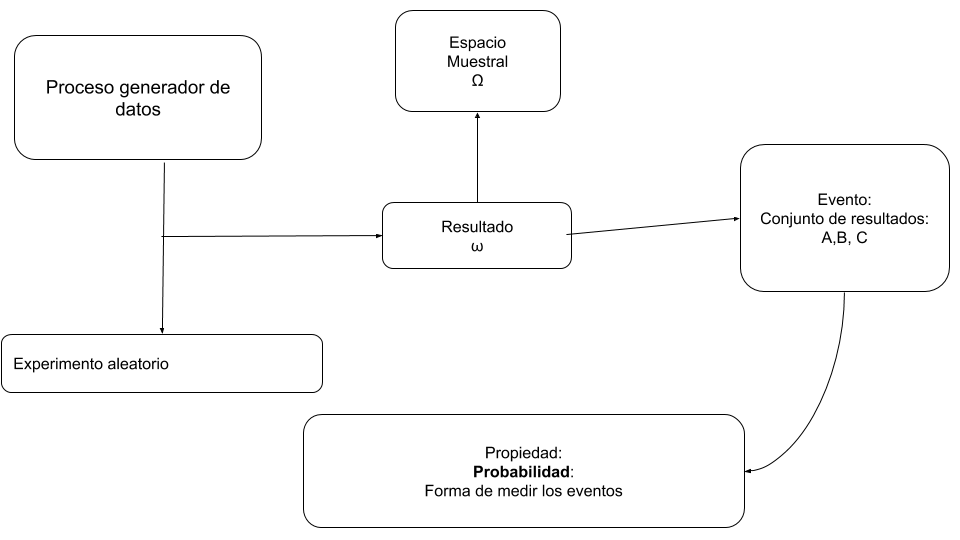
\includegraphics[width=10.41667in,height=\textheight]{img/marco_proba.png}

\begin{itemize}
\tightlist
\item
  El análisis de las probabilidades parte de un \textbf{proceso generador de datos} entendido como cualquier fenómeno que produce algún tipo de información de forma sistemática.
\item
  Cada iteración de este proceso produce información, que podemos interpretar como un \textbf{resultado}.
\item
  Existe un conjunto de posibles resultados, que definimos como \textbf{espacio muestral}.
\item
  Un \textbf{evento} es el conjunto de resultados ocurridos.
\item
  En este marco, la \textbf{probabilidad} es un atributo de los eventos. Es la forma de medir los eventos tal que, siguiendo la definición moderna de probabilidad:
\end{itemize}

\begin{enumerate}
\def\labelenumi{\Alph{enumi})}
\tightlist
\item
  \(P(A) \geq 0 \forall \ A \subseteq \Omega\)
\item
  \(P(\Omega)=1\)
\item
  \(P(A\cup B) = P(A) + P(B)\ si\ A \cap B = \emptyset\)
\end{enumerate}

\begin{quote}
ejemplo, tiramos un dado y sale tres
\end{quote}

\begin{itemize}
\tightlist
\item
  Espacio muestral: 1,2,3,4,5,6
\item
  Resultado: 3
\item
  Evento: impar (el conjunto 1,3,5)
\end{itemize}

\hypertarget{distribucion-de-probabilidad}{%
\subsubsection{Distribución de probabilidad}\label{distribucion-de-probabilidad}}

\begin{itemize}
\item
  La distribución de probabilidad hace referencia a los posibles valores teóricos de cada uno de los resultados pertenecientes al espacio muestral.
\item
  Existen dos tipos de distribuciones, dependiendo si el espacio muestral es o no numerable.
\end{itemize}

\hypertarget{distribuciones-discretas}{%
\paragraph{Distribuciones discretas}\label{distribuciones-discretas}}

Sigamos con el ejemplo de dado.

Podríamos definir la distribución de probabilidad, si el dado no está cargado, como:

\begin{verbatim}
## # A tibble: 6 x 2
##   valor probabilidad
##   <int> <chr>       
## 1     1 1/6         
## 2     2 1/6         
## 3     3 1/6         
## 4     4 1/6         
## 5     5 1/6         
## 6     6 1/6
\end{verbatim}

Como el conjunto de resultados posibles es acotado, podemos definirlo en una tabla, esta es una distribución \emph{discreta}.

\hypertarget{distribuciones-continuas}{%
\paragraph{Distribuciones continuas}\label{distribuciones-continuas}}

¿Qué pasa cuando el conjunto de resultados posibles es tan grande que no se puede enumerar la probabilidad de cada caso?

Si, por definición o por practicidad, no se puede enumerar cada caso, lo que tenemos es una \textbf{distribución continua}

\begin{quote}
Por ejemplo, la altura de la población
\end{quote}

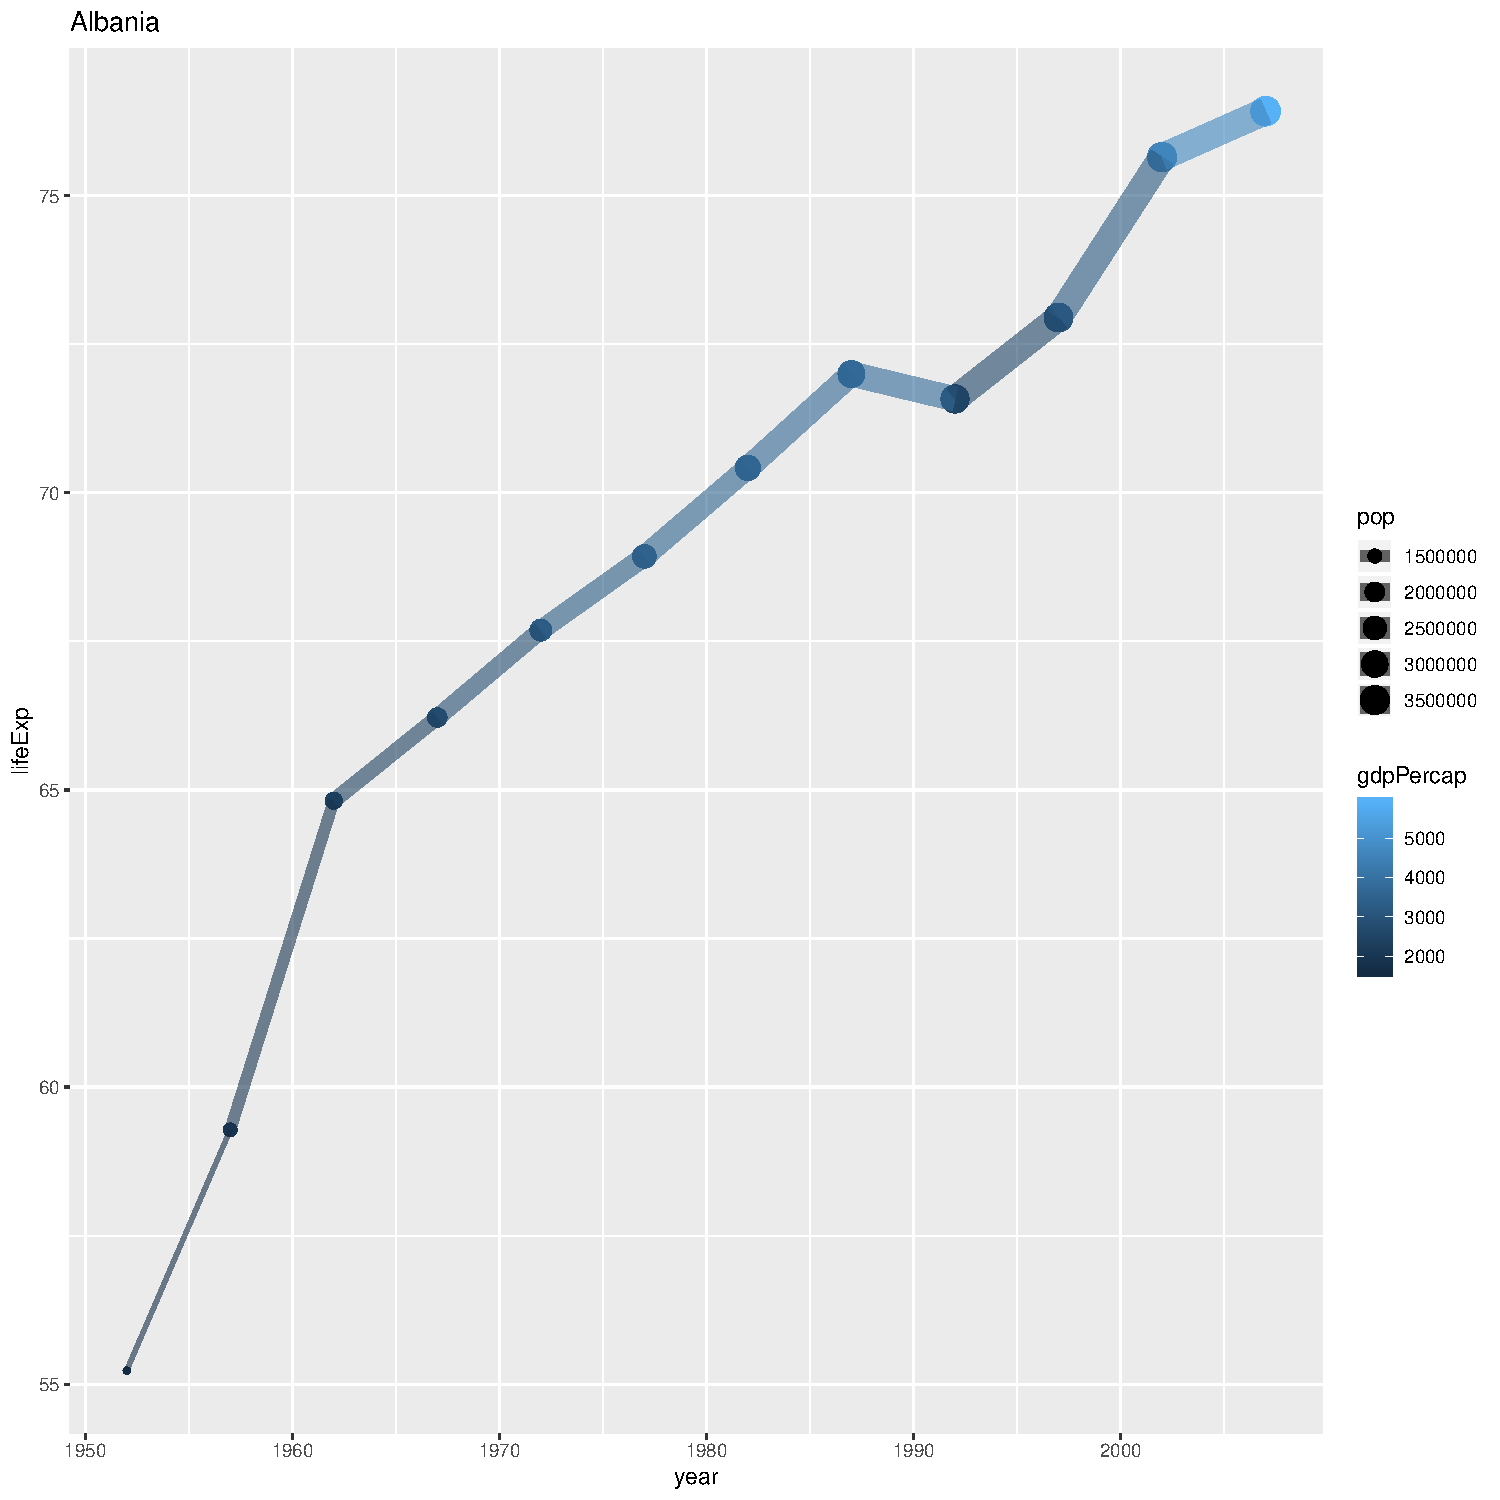
\includegraphics{bookdown_files/figure-latex/unnamed-chunk-104-1.pdf}

\begin{itemize}
\item
  En este caso, no podemos definir en una tabla la probabilidad de cada uno de los posibles valores. \emph{de hecho, la probabilidad puntual es 0}.
\item
  Sin embargo, sí podemos definir una \emph{función de probabilidad}, la \emph{densidad}.
\item
  Según qué función utilicemos, cambiará la forma de la curva.
\end{itemize}

Por ejemplo:

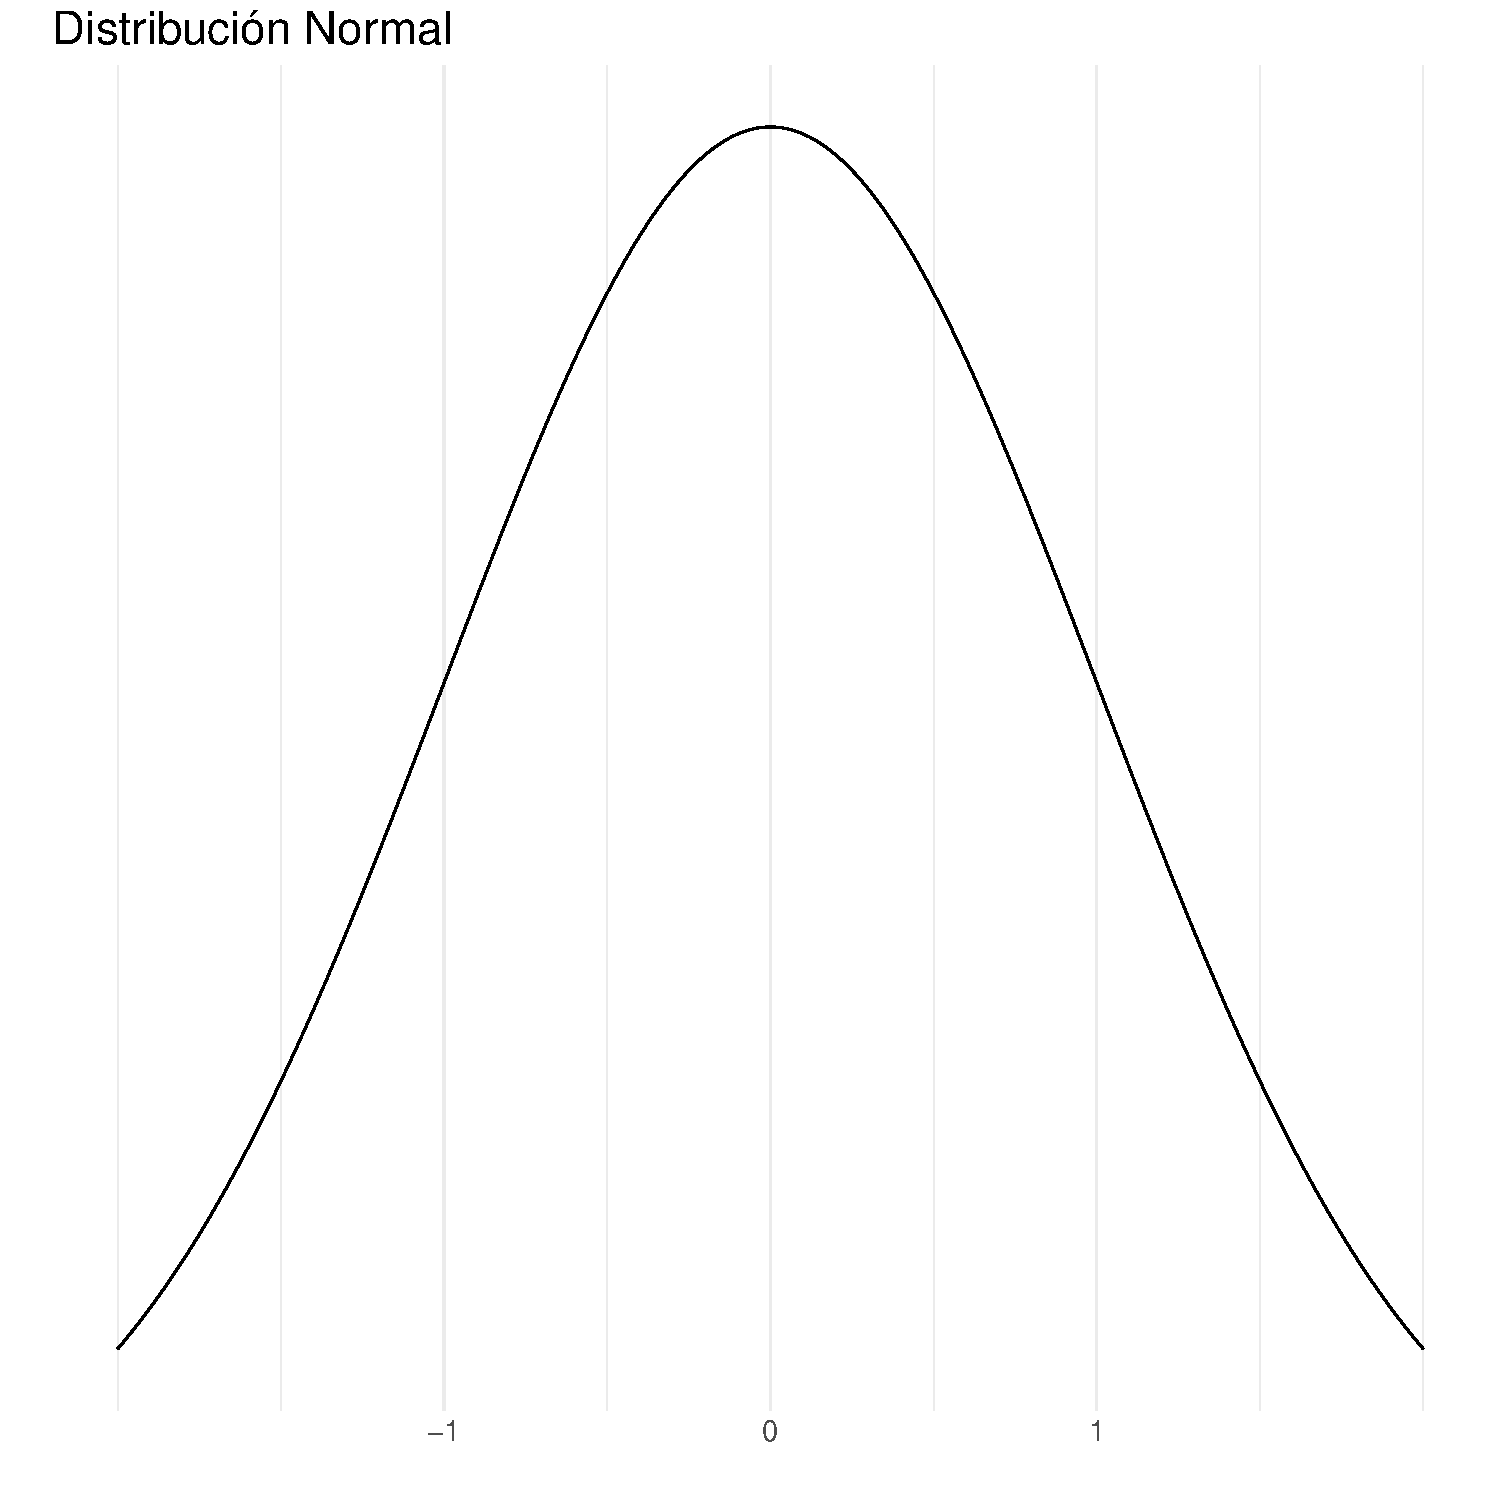
\includegraphics{bookdown_files/figure-latex/unnamed-chunk-105-1.pdf} 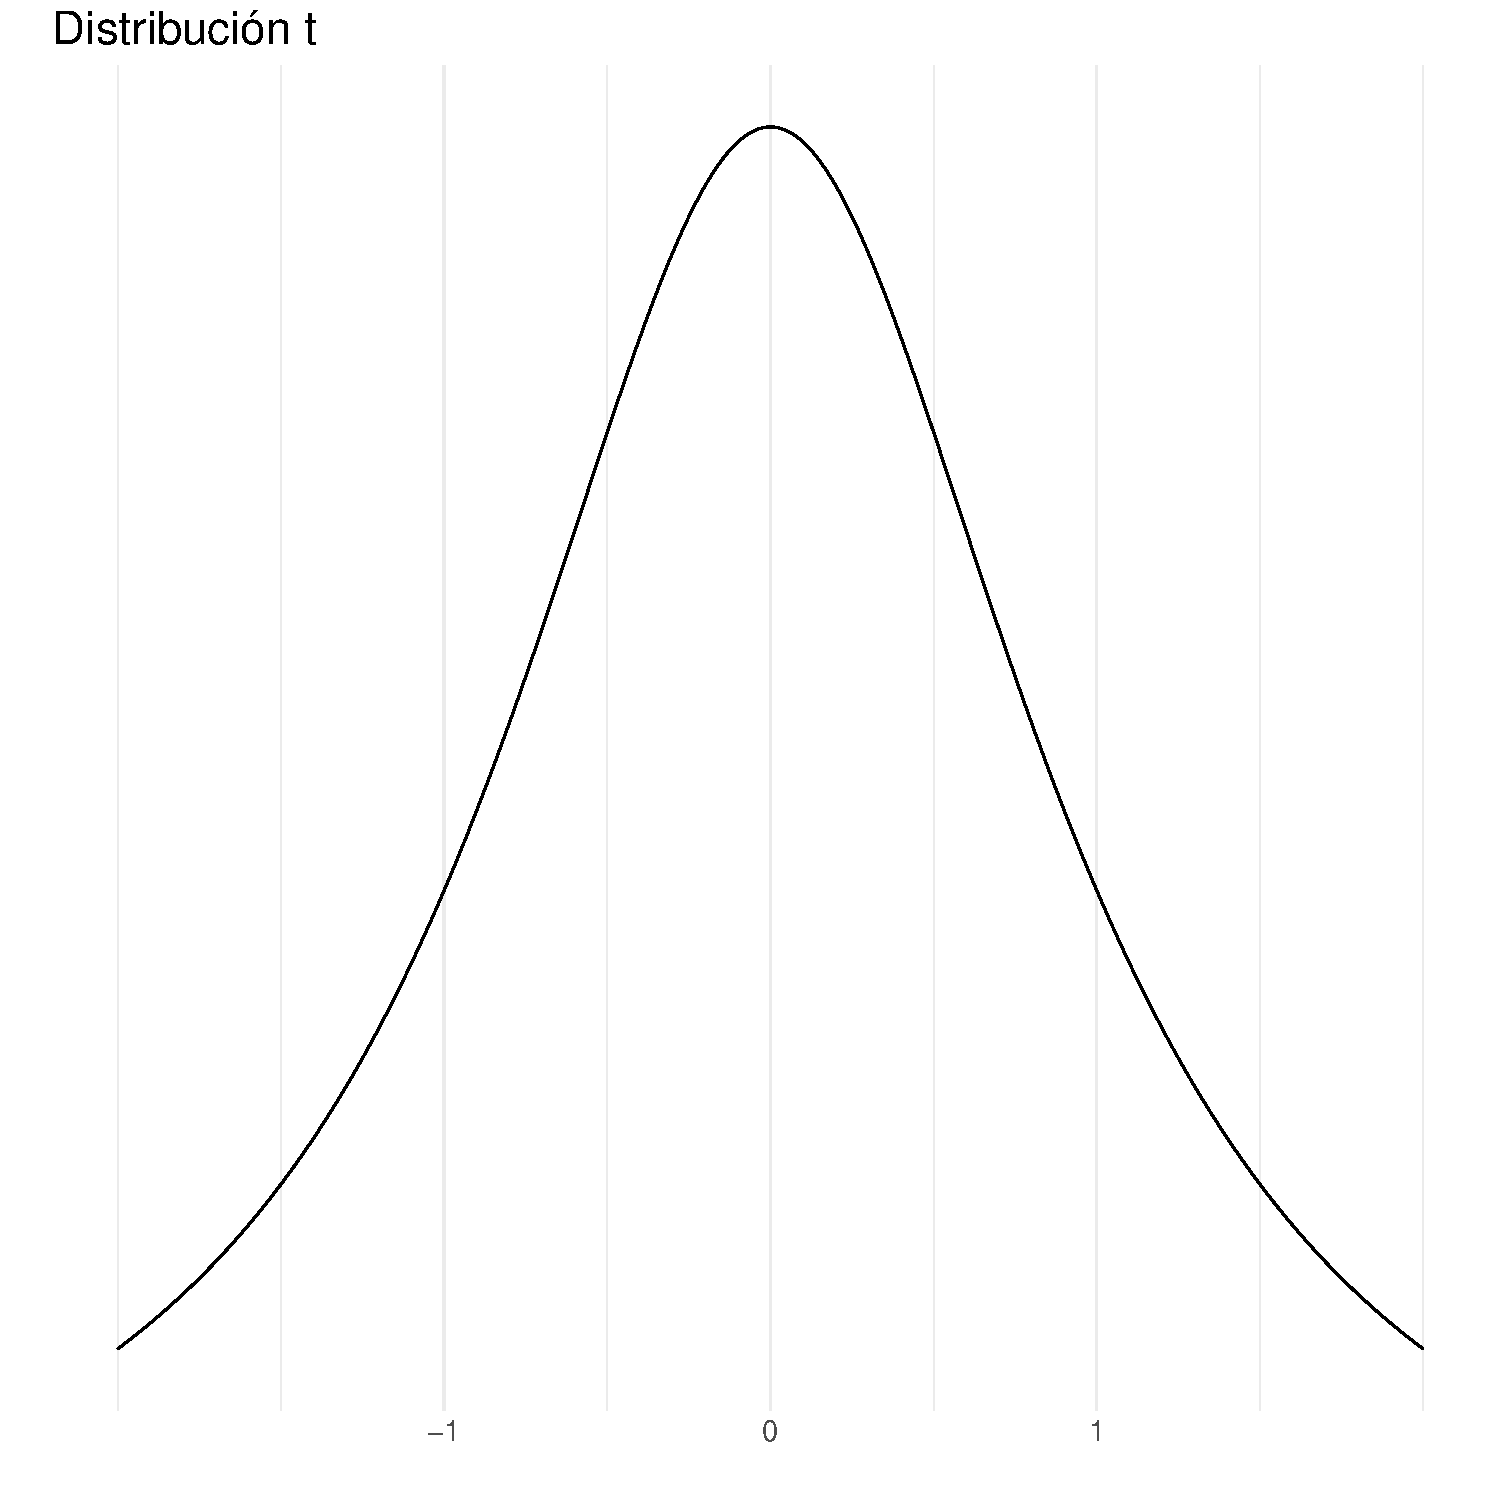
\includegraphics{bookdown_files/figure-latex/unnamed-chunk-105-2.pdf} 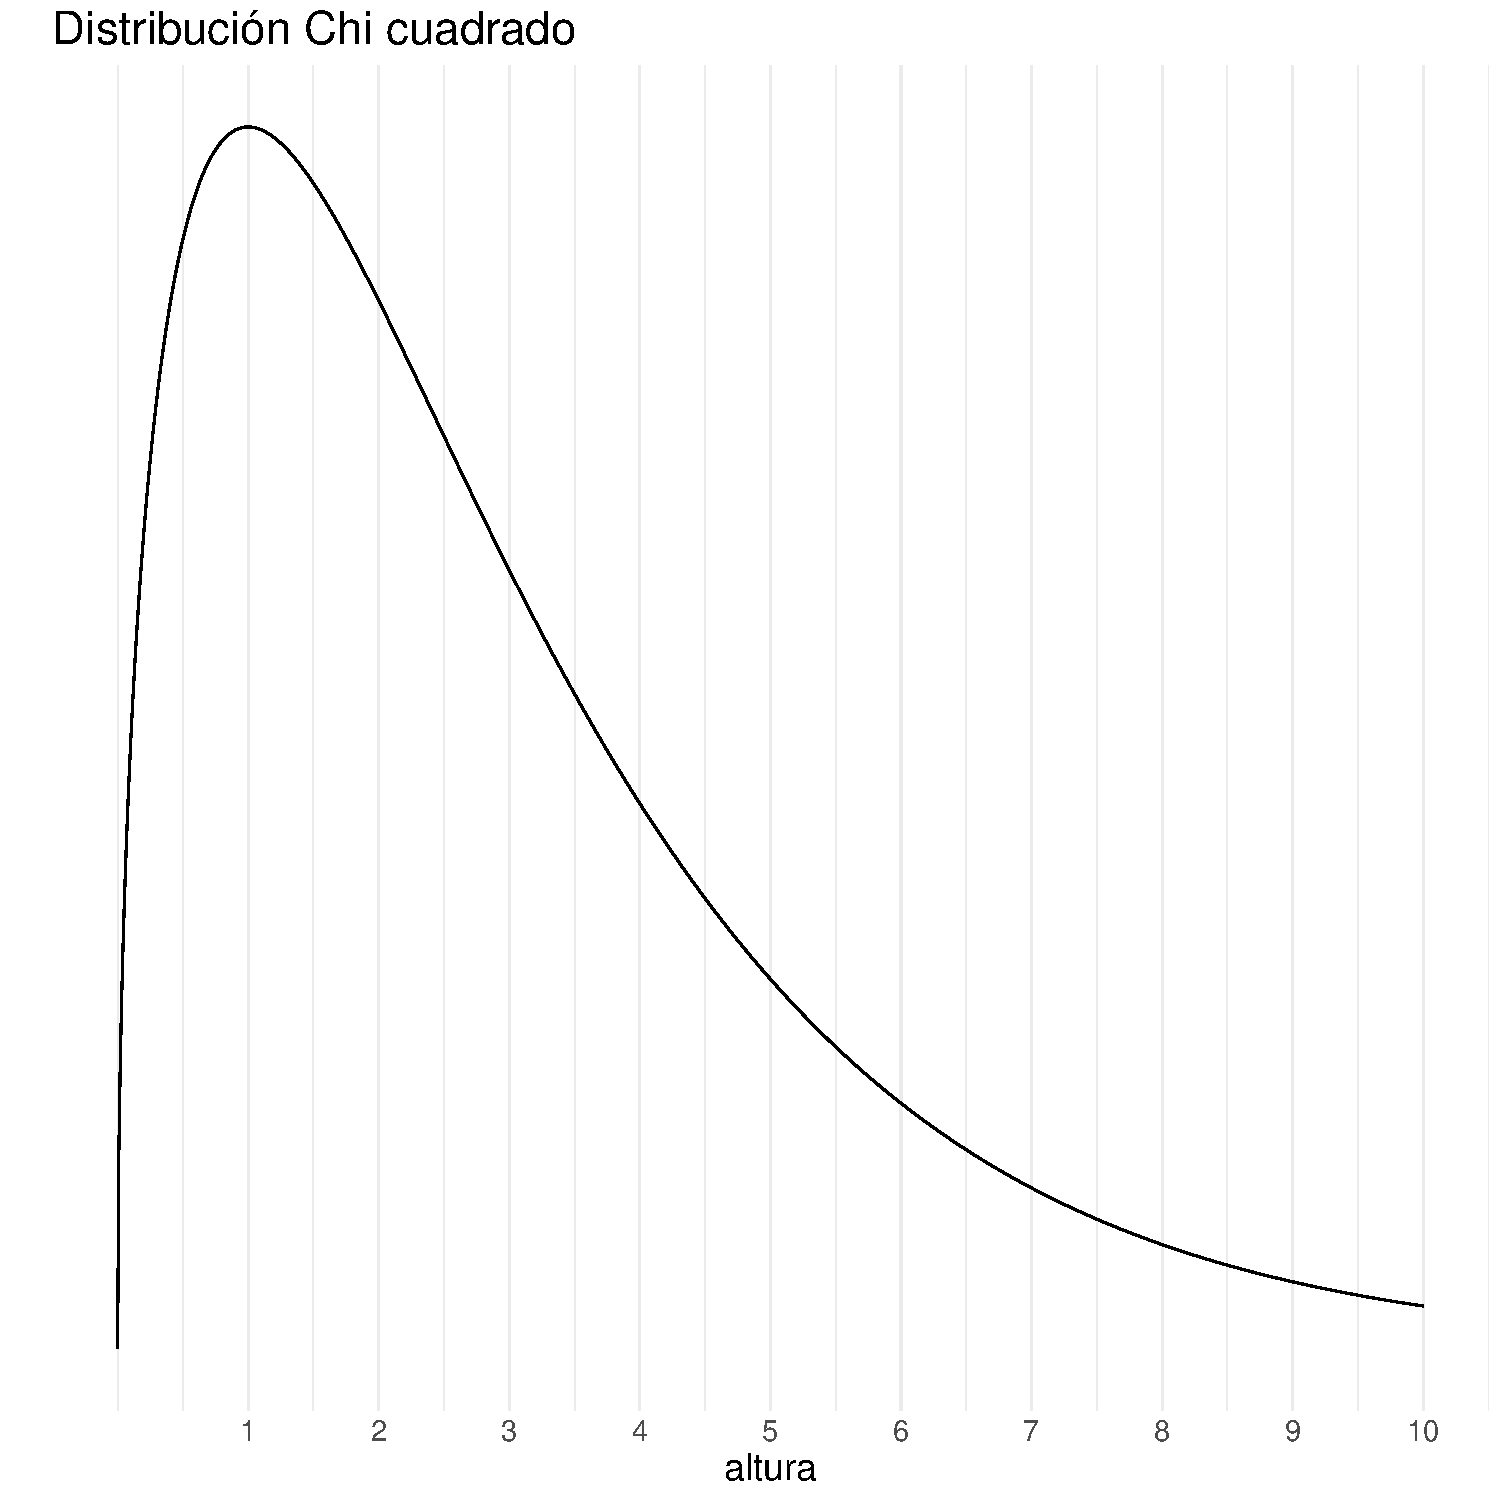
\includegraphics{bookdown_files/figure-latex/unnamed-chunk-105-3.pdf}

\begin{quote}
Una distribución de probabilidad se \textbf{caracteriza} por sus \emph{parámetros}.
\end{quote}

\begin{itemize}
\tightlist
\item
  Por ejemplo, la distribución normal se caracteriza por su \emph{esperanza} y su \emph{varianza} (o desvío estándar)
\end{itemize}

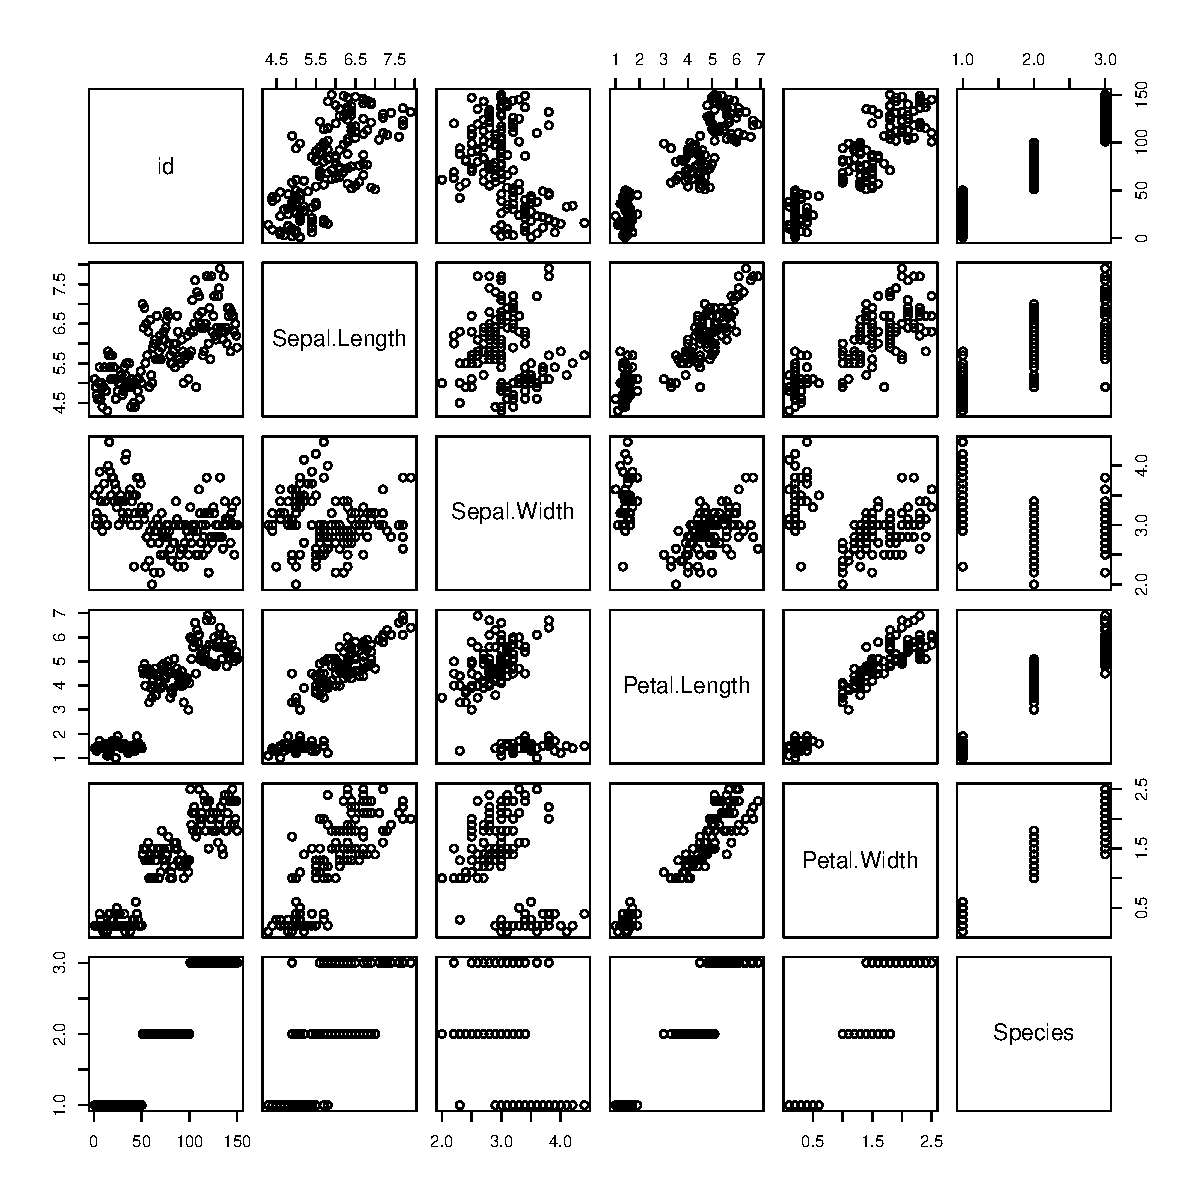
\includegraphics{bookdown_files/figure-latex/unnamed-chunk-106-1.pdf} 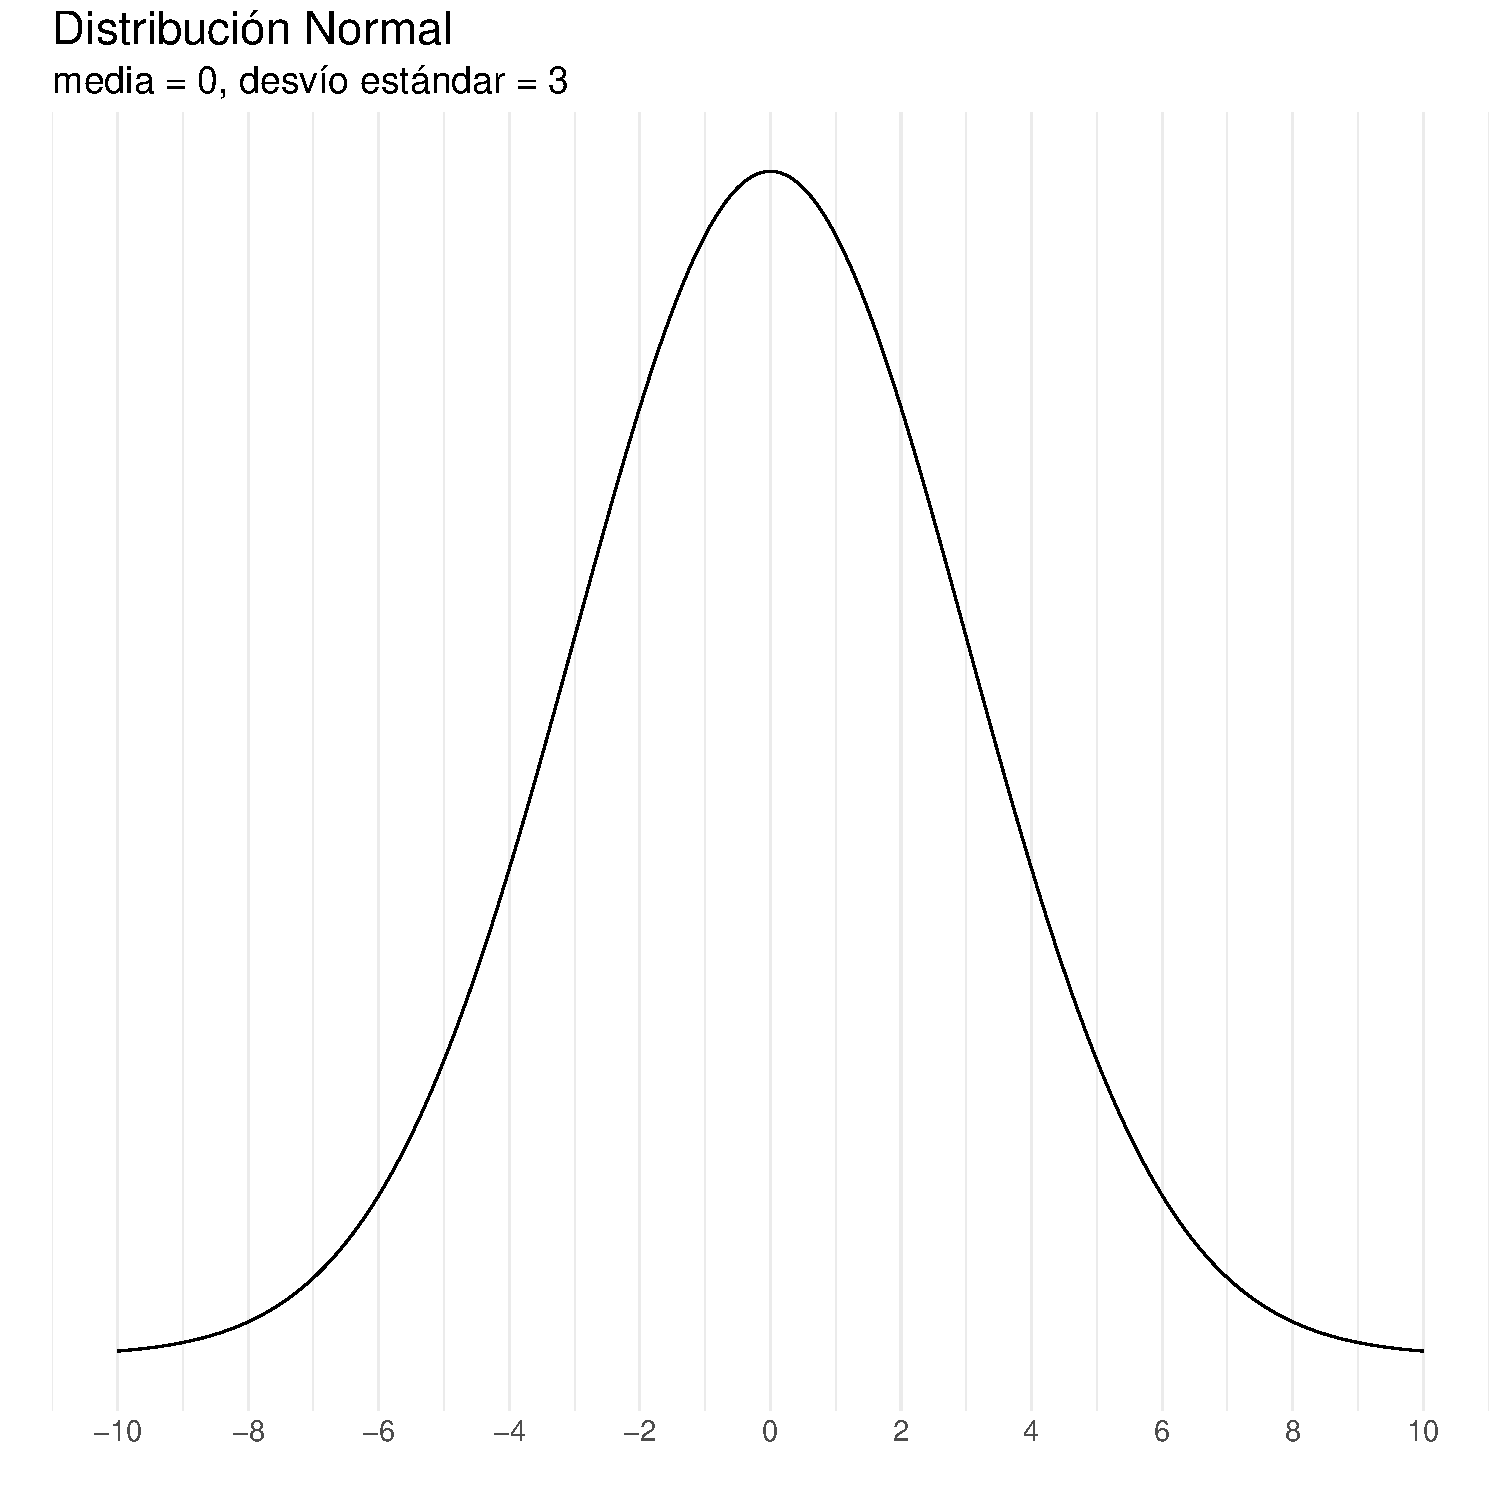
\includegraphics{bookdown_files/figure-latex/unnamed-chunk-106-2.pdf} 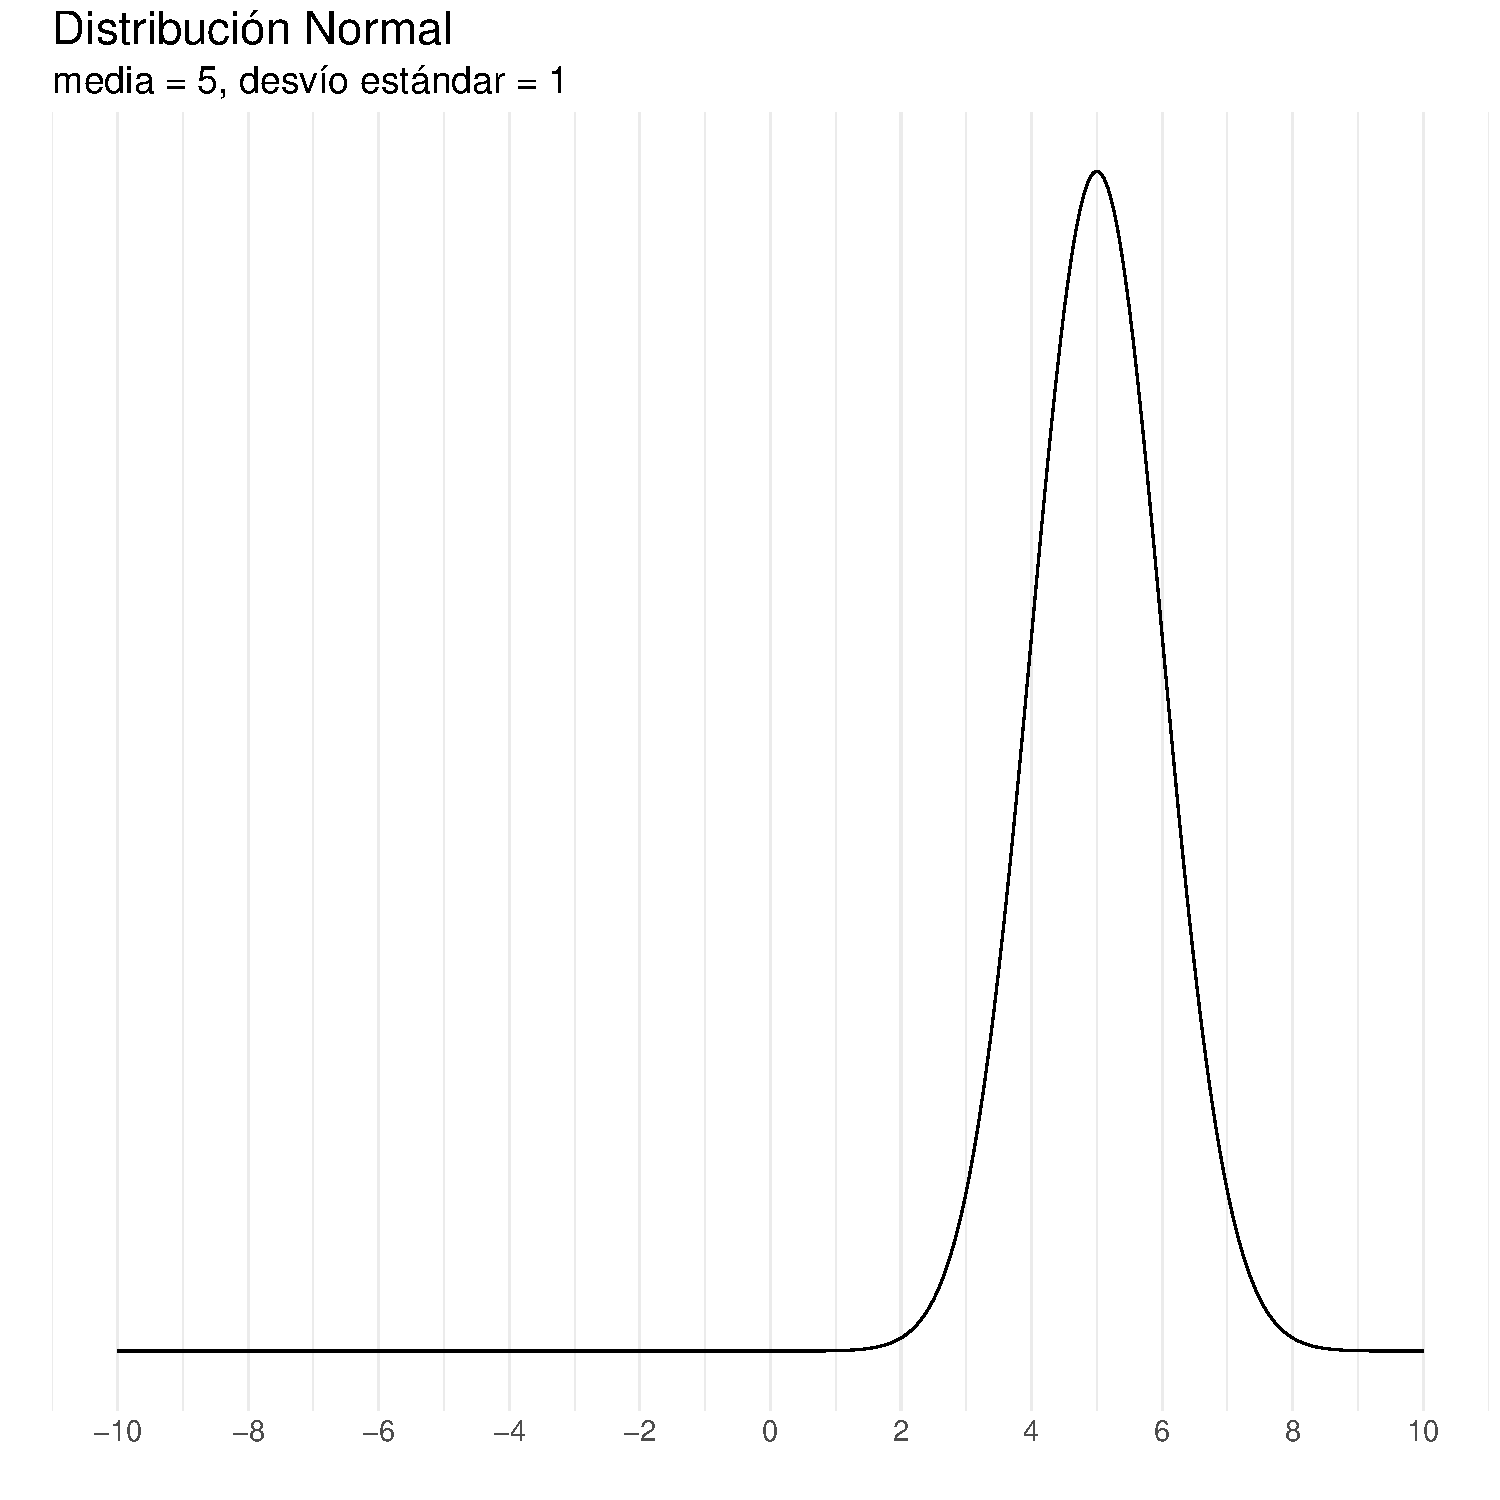
\includegraphics{bookdown_files/figure-latex/unnamed-chunk-106-3.pdf}

\hypertarget{estadistica}{%
\subsection{Estadística}\label{estadistica}}

\hypertarget{el-problema-de-la-inversion}{%
\subsubsection{El problema de la inversión}\label{el-problema-de-la-inversion}}

El problema de la probabilidad se podría pensar de la siguiente forma:

\begin{enumerate}
\def\labelenumi{\arabic{enumi}.}
\tightlist
\item
  Vamos a partir de un \textbf{proceso generador de datos}
\item
  Para calcular su \textbf{distribución de probabilidad}, los \textbf{parámetros} que caracterizan a ésta, y a partir de allí,
\item
  Calcular la probabilidad de que, al tomar una \textbf{muestra}, tenga ciertos eventos.
\end{enumerate}

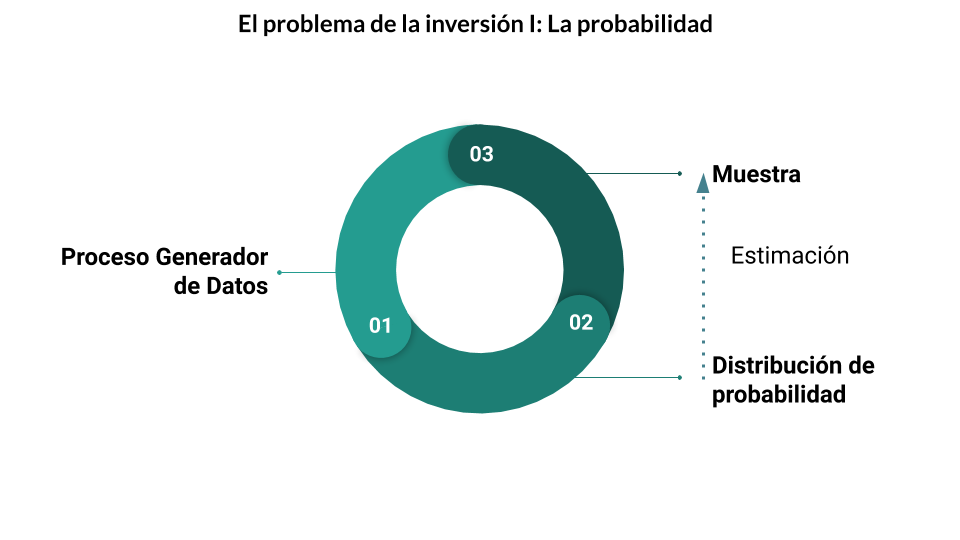
\includegraphics[width=10.41667in,height=\textheight]{img/problema_inversion_1.png}

El problema de la estadística es exactamente el contrario:

\begin{enumerate}
\def\labelenumi{\arabic{enumi}.}
\tightlist
\item
  Partimos de una \textbf{muestra} para
\item
  Inferir cuál es la \textbf{distribución de probabilidad}, y los \textbf{parámetros} que la caracterizan
\item
  Para finalmente poder sacar conclusiones sobre el \textbf{proceso generador de datos}
\end{enumerate}

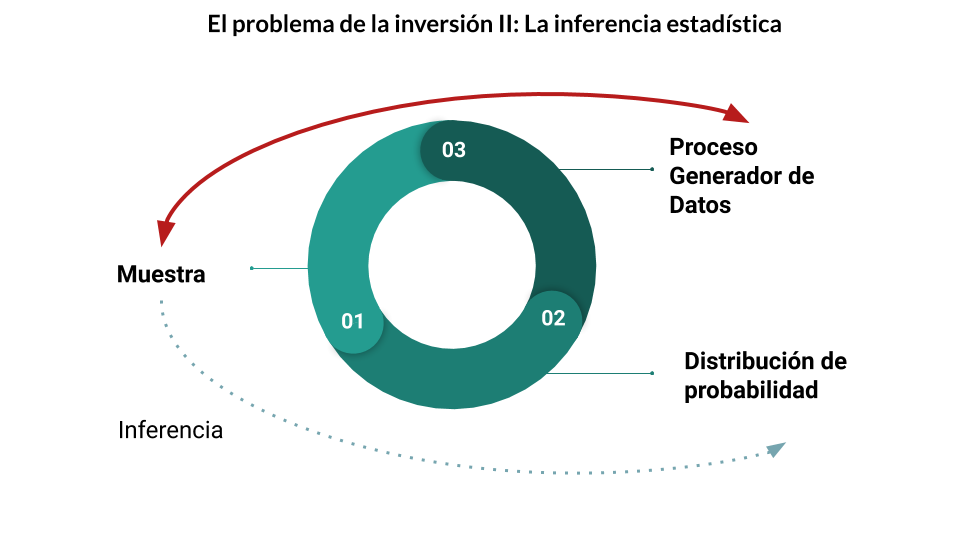
\includegraphics[width=10.41667in,height=\textheight]{img/problema_inversion_2.png}

\hypertarget{poblacion-y-muestra}{%
\paragraph{Población y muestra}\label{poblacion-y-muestra}}

En este punto podemos hacer la distinción entre \textbf{población} y \textbf{muestra}

\begin{itemize}
\tightlist
\item
  \textbf{Población}: El universo en estudio. Puede ser:

  \begin{itemize}
  \tightlist
  \item
    finita: Los votantes en una elección.
  \item
    infinita: El lanzamiento de una moneda.
  \end{itemize}
\item
  \textbf{Muestra}: subconjunto de n observaciones de una población.
\end{itemize}

Solemos utilizar las mayúsculas (N) para la población y las minúsculas (n) para las muestras

\hypertarget{parametros-y-estimadores}{%
\paragraph{Parámetros y Estimadores}\label{parametros-y-estimadores}}

\begin{itemize}
\tightlist
\item
  Como dijimos, los \textbf{parámetros} describen a la función de probabilidad. Por lo tanto hacen referencia a los atributos de la \textbf{población}. Podemos suponer que son \emph{constantes}.
\item
  Un \textbf{estimador} es un estadístico (esto es, una función de la muestra) usado para estimar un parámetro desconocido de la población.
\end{itemize}

\hypertarget{ejemplo.-la-media}{%
\paragraph{Ejemplo. La media}\label{ejemplo.-la-media}}

Esperanza o Media Poblacional:

\[
\mu = E(x)= \sum_{i=1}^N x_ip(x_i)
\]

Media muestral:

\[
\bar{X}= \sum_{i=1}^n \frac{Xi}{n}
\]

Como no puedo conocer \(\mu\), lo estimo mediante \(\bar{X}\)

\hypertarget{estimacion-puntual-intervalos-de-confianza-y-tests-de-hipotesis}{%
\subsubsection{Estimación puntual, Intervalos de confianza y Tests de hipótesis}\label{estimacion-puntual-intervalos-de-confianza-y-tests-de-hipotesis}}

\begin{itemize}
\item
  El estimador \(\bar{X}\) nos devuelve un número. Esto es una inferencia de cuál creemos que es la media. Pero no es seguro que esa sea realmente la media. Esto es lo que denominamos estimación puntual.
\item
  También podemos estimar un intervalo, dentro del cual consideramos que se encuentra la media poblacional. La ventaja de esta metodología es que podemos definir la probabilidad de que el parámetro poblacional realmente esté dentro de este intervalo. Esto se conoce como \textbf{intervalos de confianza}.
\item
  Por su parte, también podemos calcular la probabilidad de que el parámetro poblacional sea mayor, menor o igual a un cierto valor. Esto es lo que se conoce como \textbf{test de hipótesis}.
\item
  En el fondo, los intervalos de confianza y los tests de hipótesis se construyen de igual manera. Son funciones que se construyen a partir de los datos, que se comparan con distribuciones conocidas, \emph{teóricas}.
\end{itemize}

\hypertarget{definicion-de-los-tests}{%
\paragraph{Definición de los tests}\label{definicion-de-los-tests}}

\begin{itemize}
\tightlist
\item
  Los tests se construyen con dos hipótesis: La hipótesis nula \(H_0\), y la hipótesis alternativa, \(H_1\). Lo que buscamos es ver si \emph{hay evidencia suficiente para rechazar la hipótesis nula}.
\end{itemize}

Por ejemplo, si queremos comprobar si la media poblacional, \(\mu\) de una distribución es mayor a \(X_i\), haremos un test con las siguientes hipótesis:

\begin{itemize}
\tightlist
\item
  \(H_0: \mu = X_i\)
\item
  \(H_1: \mu > X_i\)
\end{itemize}

Si la evidencia es lo suficientemente fuerte, podremos rechazar la hipótesis \(H_0\), \emph{pero no afirmar la hipótesis \(H_1\)}

\hypertarget{significatividad-en-los-tests}{%
\paragraph{Significatividad en los tests}\label{significatividad-en-los-tests}}

\begin{itemize}
\item
  Muchas veces decimos que algo es \textbf{``estadísticamente significativo''}. Detrás de esto se encuentra un test de hipótesis que indica que hay una suficiente \emph{significativdad estadística}.
\item
  La \emph{significatividad estadística}, representada con \(\alpha\), es la probabilidad de rechazar \(H_0\) cuando en realidad es cierta. Por eso, cuanto más bajo el valor de \(\alpha\), más seguros estamos de no equivocarnos. Por lo general testeamos con valores de alpha de 1\%, 5\% y 10\%, dependiendo del área de estudio.
\item
  El \textbf{p-valor} es \emph{la mínima significatividad} para la que rechazo el test. Es decir, cuanto más bajo es el p-valor, más seguros estamos de rechazar \(H_0\).
\item
  El resultado de un test está determinado por:

  \begin{enumerate}
  \def\labelenumi{\arabic{enumi}.}
  \tightlist
  \item
    \textbf{La fuerza de la evidencia empírica}: Si nuestra duda es si la media poblacional es mayor a, digamos, 10, y la media muestral es 11, no es lo mismo que si es 100, 1000 o 10000.
  \item
    \textbf{El tamaño de la muestra}: En las fórmulas que definen los test siempre juega el tamaño de la muestra: cuanto más grande es, más seguros estamos de que el resultado no es producto del mero azar.
  \item
    \textbf{La veracidad de los supuestos}: Otra cosa importante es que los test asumen ciertas cosas:
  \end{enumerate}

  \begin{itemize}
  \tightlist
  \item
    Normalidad en los datos.
  \item
    Que conocemos algún otro parámetro de la distribución, como la varianza.
  \item
    Que los datos son independientes entre sí,
  \item
    Etc.\\
    \textbf{Cada Test tiene sus propios supuestos}. Por eso a veces, luego de hacer un test, hay que hacer otros tests para validar que los supuestos se cumplen.
  \end{itemize}
\item
  Lo primero, la fuerza de la evidencia, es lo que más nos importa, y no hay mucho por hacer.
\item
  El tamaño de la muestra es un problema, porque si la muestra es muy chica, entonces podemos no llegar a conclusiones significativas aunque sí ocurra aquello que queríamos probar.
\item
  Sin embargo, el verdadero problema en \emph{La era del big data} es que tenemos muestras demasiado grandes, por lo que cualquier test, por más mínima que sea la diferencia, puede dar significativo.
\end{itemize}

\begin{quote}
Por ejemplo, podemos decir que la altura promedio en Argentina es 1,74. Pero si hacemos un test, utilizando como muestra 40 millones de personas, vamos a rechazar que ese es el valor, porque en realidad es 1,7401001. En términos de lo que nos puede interesar, 1,74 sería válido, pero estadísticamente rechazaríamos.
\end{quote}

\begin{itemize}
\tightlist
\item
  Finalmente, según la información que tengamos de la población y cuál es el problema que queremos resolver, vamos a tener que utilizar distintos tipos de tests. La cantidad de tests posibles es ENORME, y escapa al contenido de este curso, así como sus fórmulas. A modo de ejemplo, les dejamos el siguiente machete:
\end{itemize}

\begin{figure}
\centering
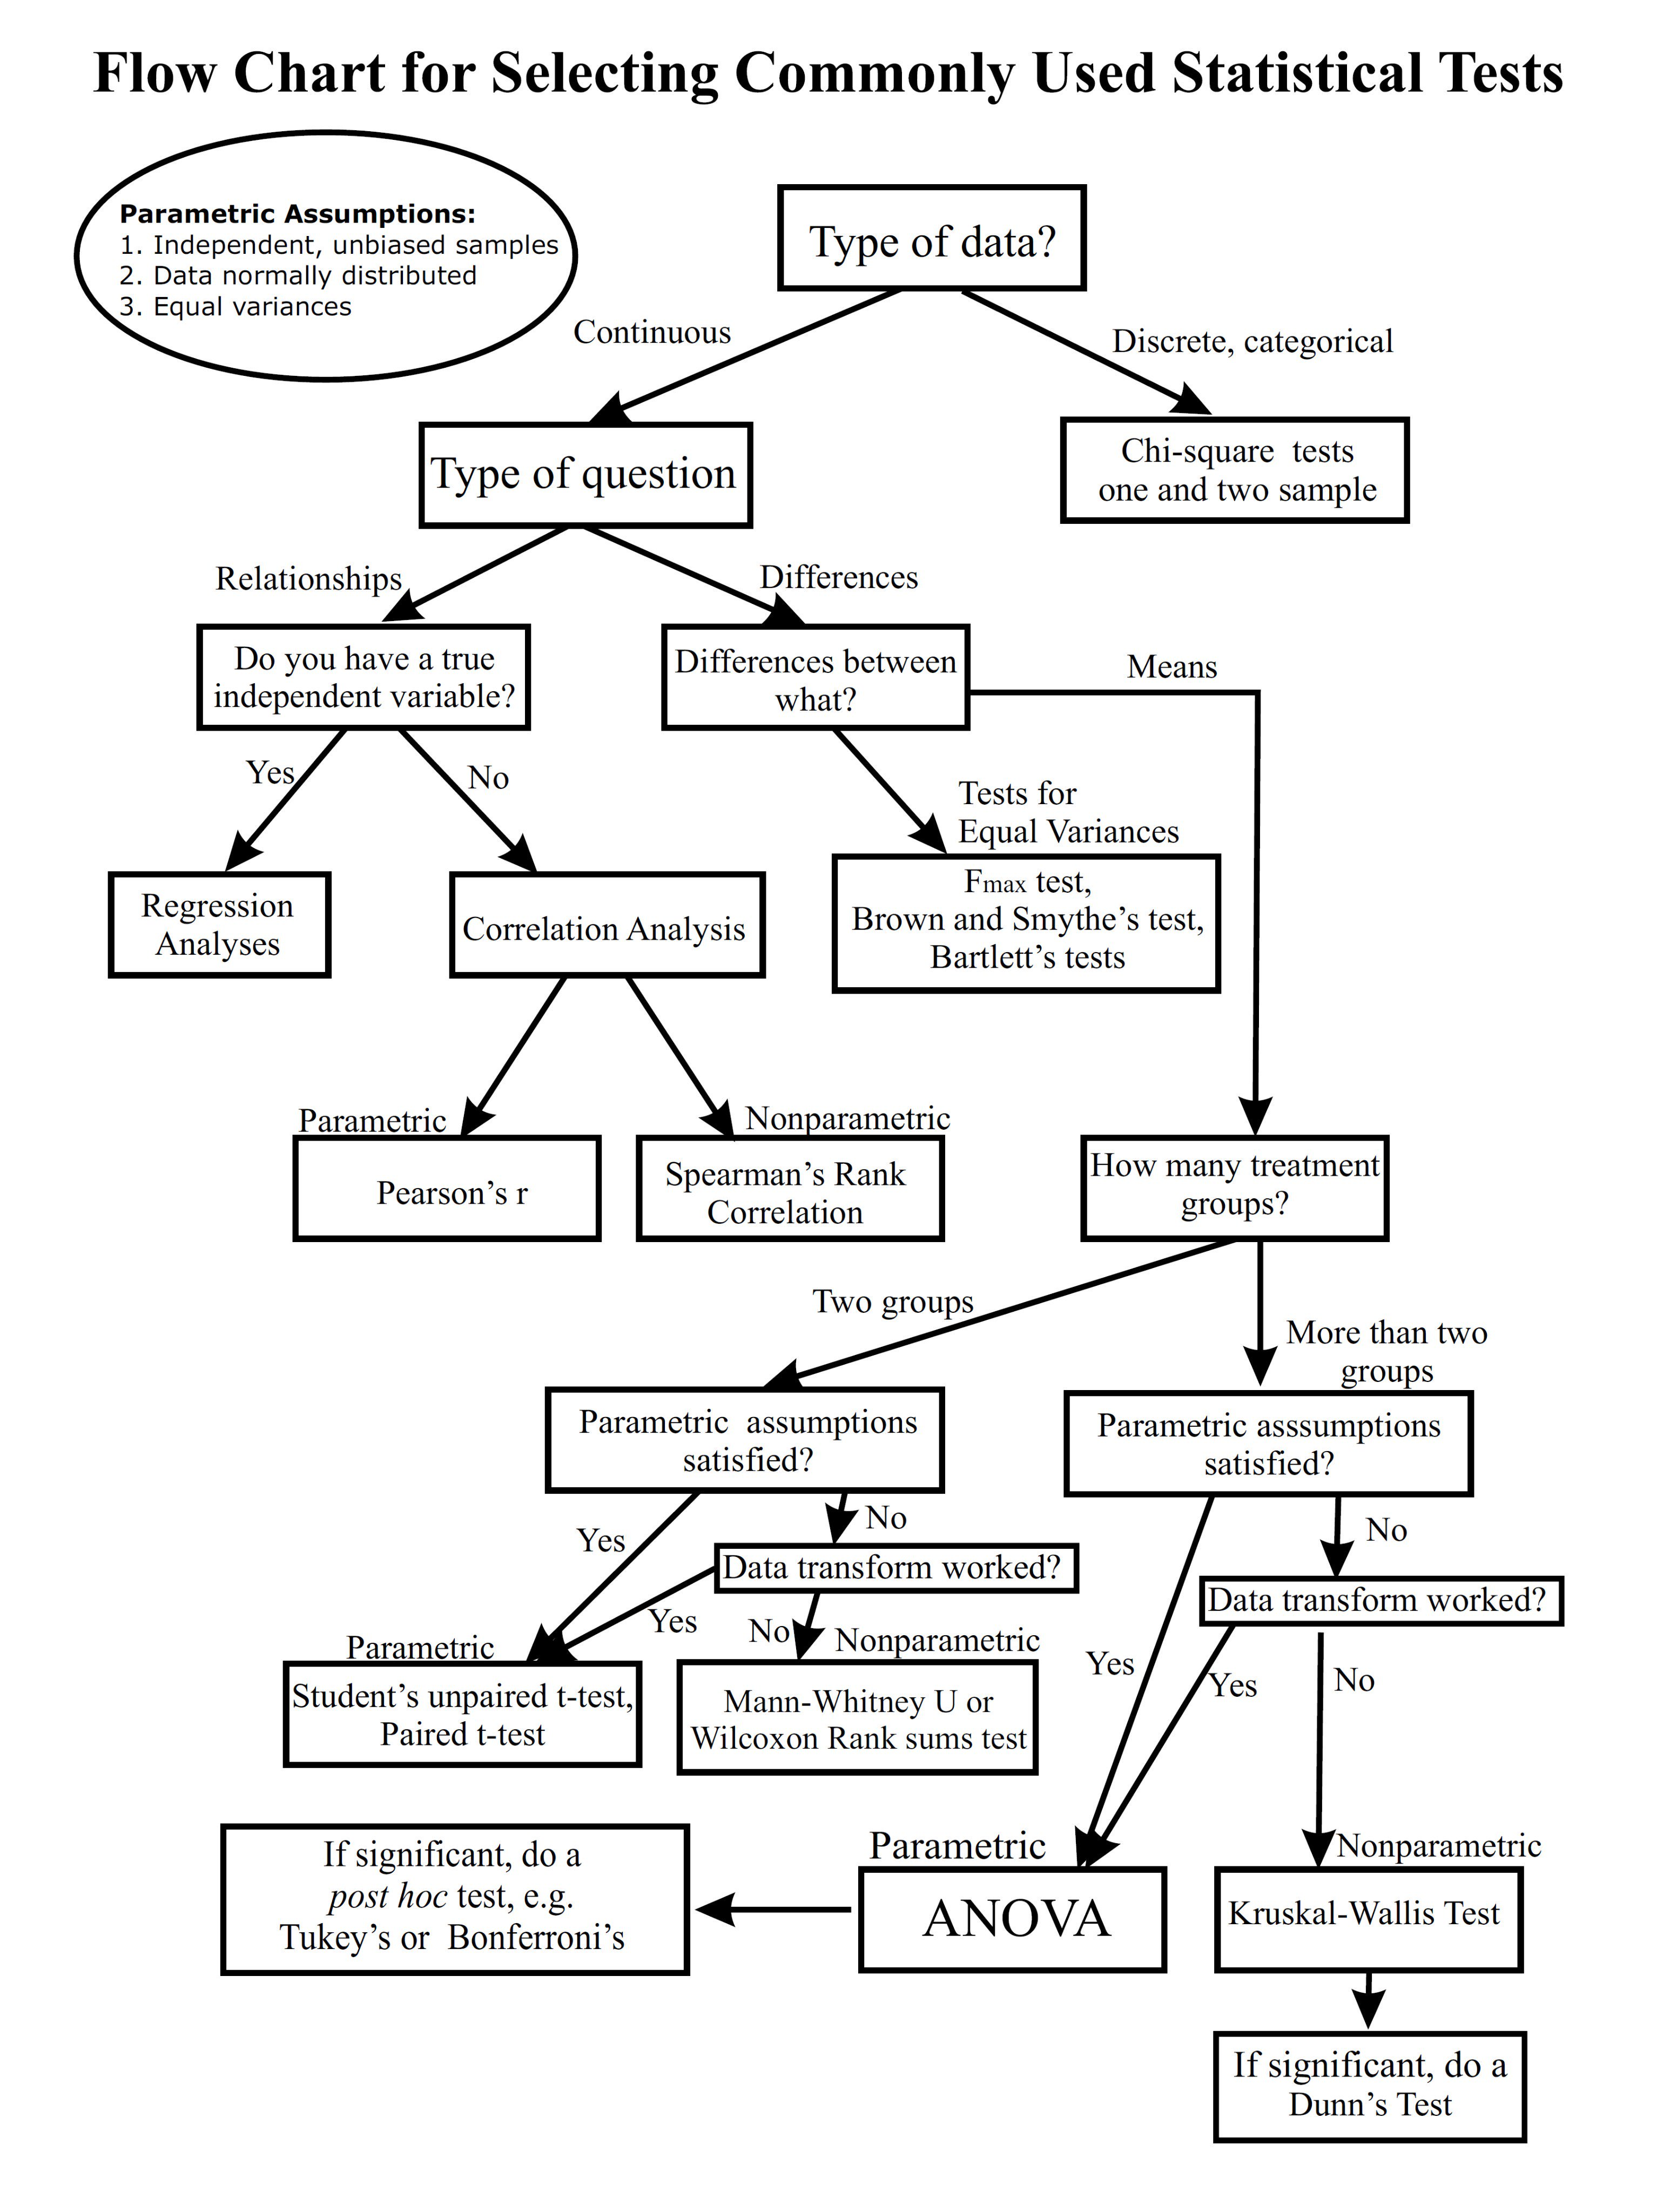
\includegraphics[width=10.41667in,height=\textheight]{img/tests.jpeg}
\caption{fuente: \url{http://abacus.bates.edu/~ganderso/biology/resources/statistics.html}}
\end{figure}

\hypertarget{algunos-estimadores-importantes}{%
\subsection{Algunos estimadores importantes}\label{algunos-estimadores-importantes}}

\hypertarget{medidas-de-centralidad}{%
\subsubsection{Medidas de centralidad}\label{medidas-de-centralidad}}

\begin{itemize}
\tightlist
\item
  \textbf{Media}
\end{itemize}

\[
\bar{X}= \sum_{i=1}^n \frac{Xi}{n}
\]

\begin{itemize}
\tightlist
\item
  \textbf{Mediana}:
\end{itemize}

Es el valor que parte la distribución a la mitad

\begin{itemize}
\tightlist
\item
  \textbf{Moda}
\end{itemize}

La moda es el valor más frecuente de la distribución

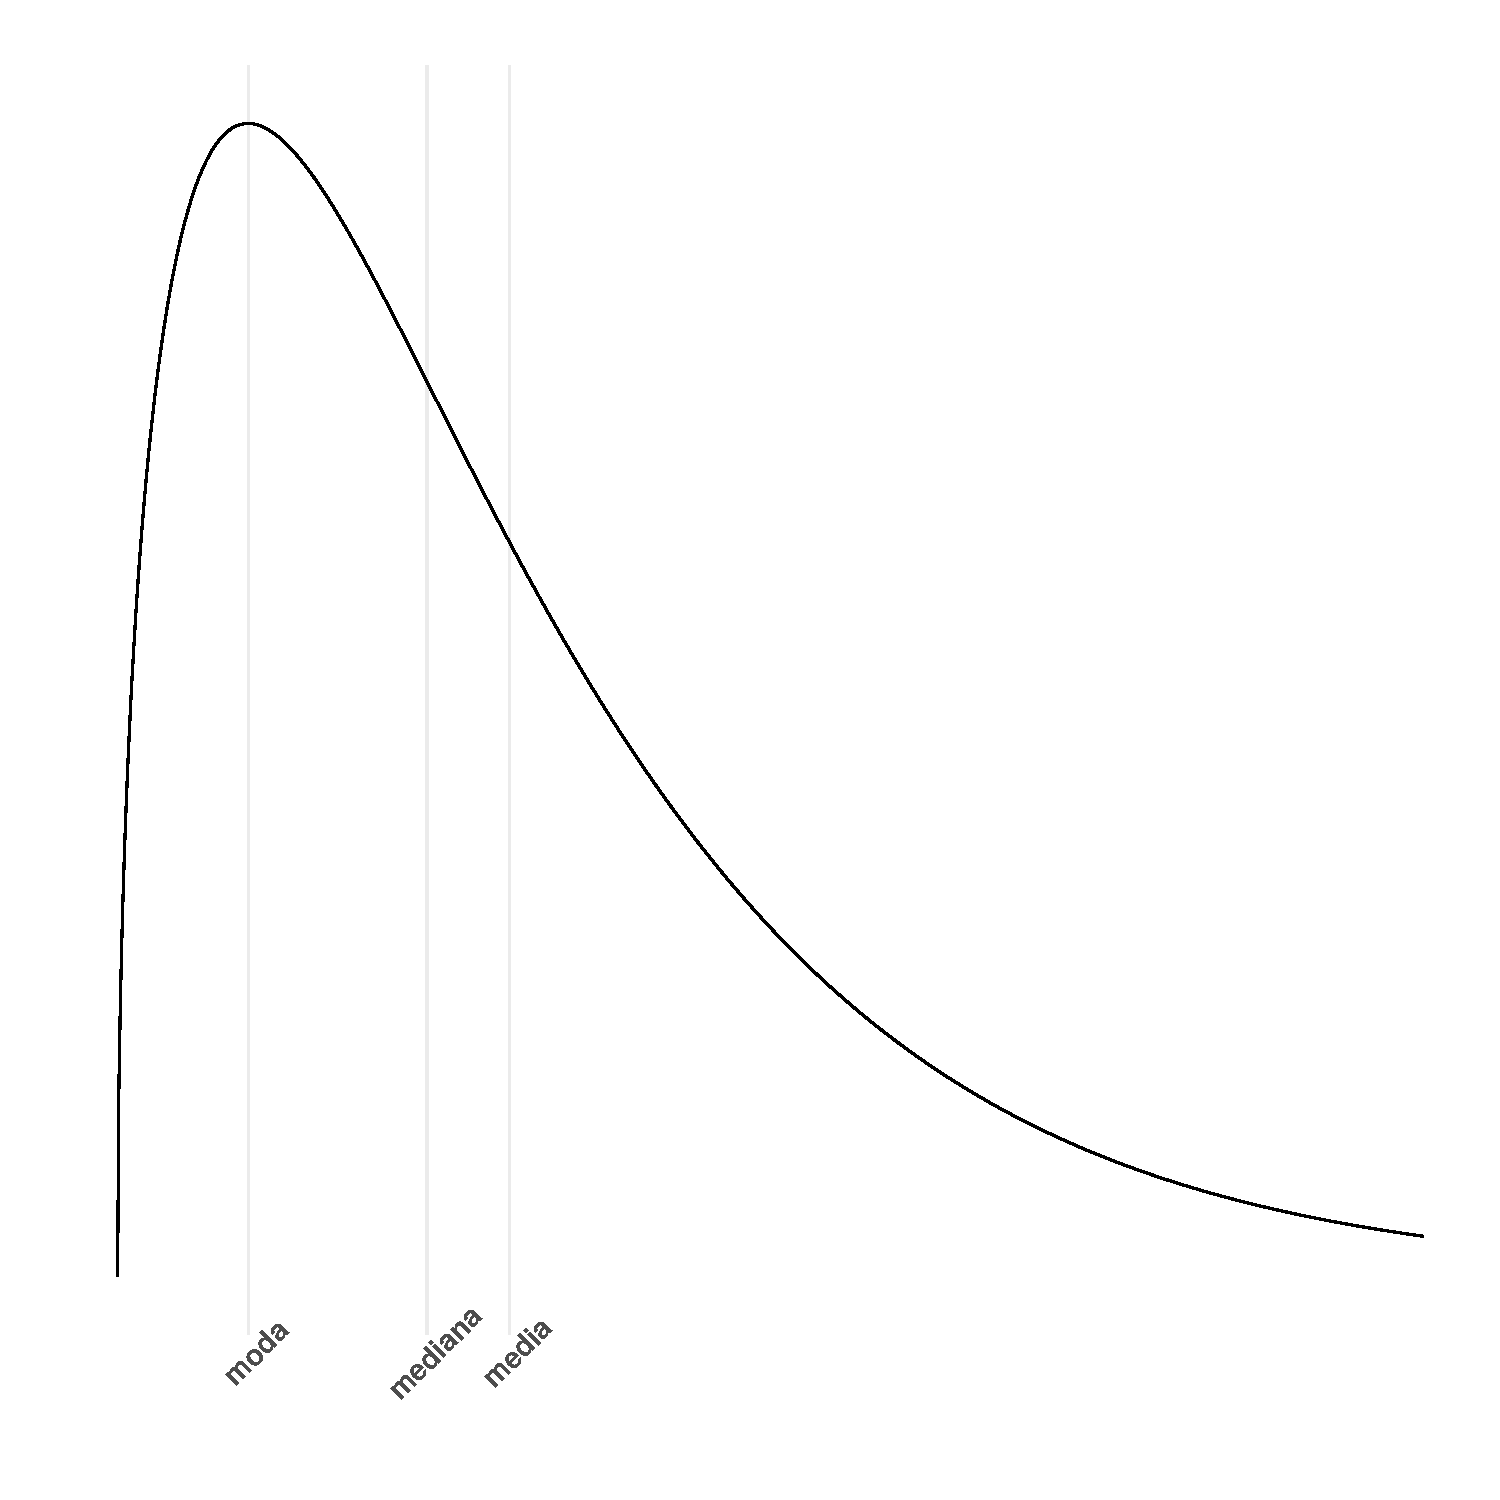
\includegraphics{bookdown_files/figure-latex/unnamed-chunk-107-1.pdf}

\hypertarget{cuantiles}{%
\subsubsection{Cuantiles}\label{cuantiles}}

Así como dijimos que la mediana es el valor que deja al 50\% de los datos de un lado y al 50\% del otro, podemos generalizar este concepto a cualquier X\%. Esto son los cuantiles. El cuantil x, es el valor tal que queda un x\% de la distribución a izquierda, y 1-x a derecha.

Algunos de los más utilizados son el del 25\%, también conocido como \(Q_1\) (el \emph{cuartil} 1), el \(Q_2\) (la mediana) y el \(Q_3\) (el \emph{cuartil} 3), que deja el 75\% de los datos a su derecha. Veamos cómo se ven en la distribución de arriba.

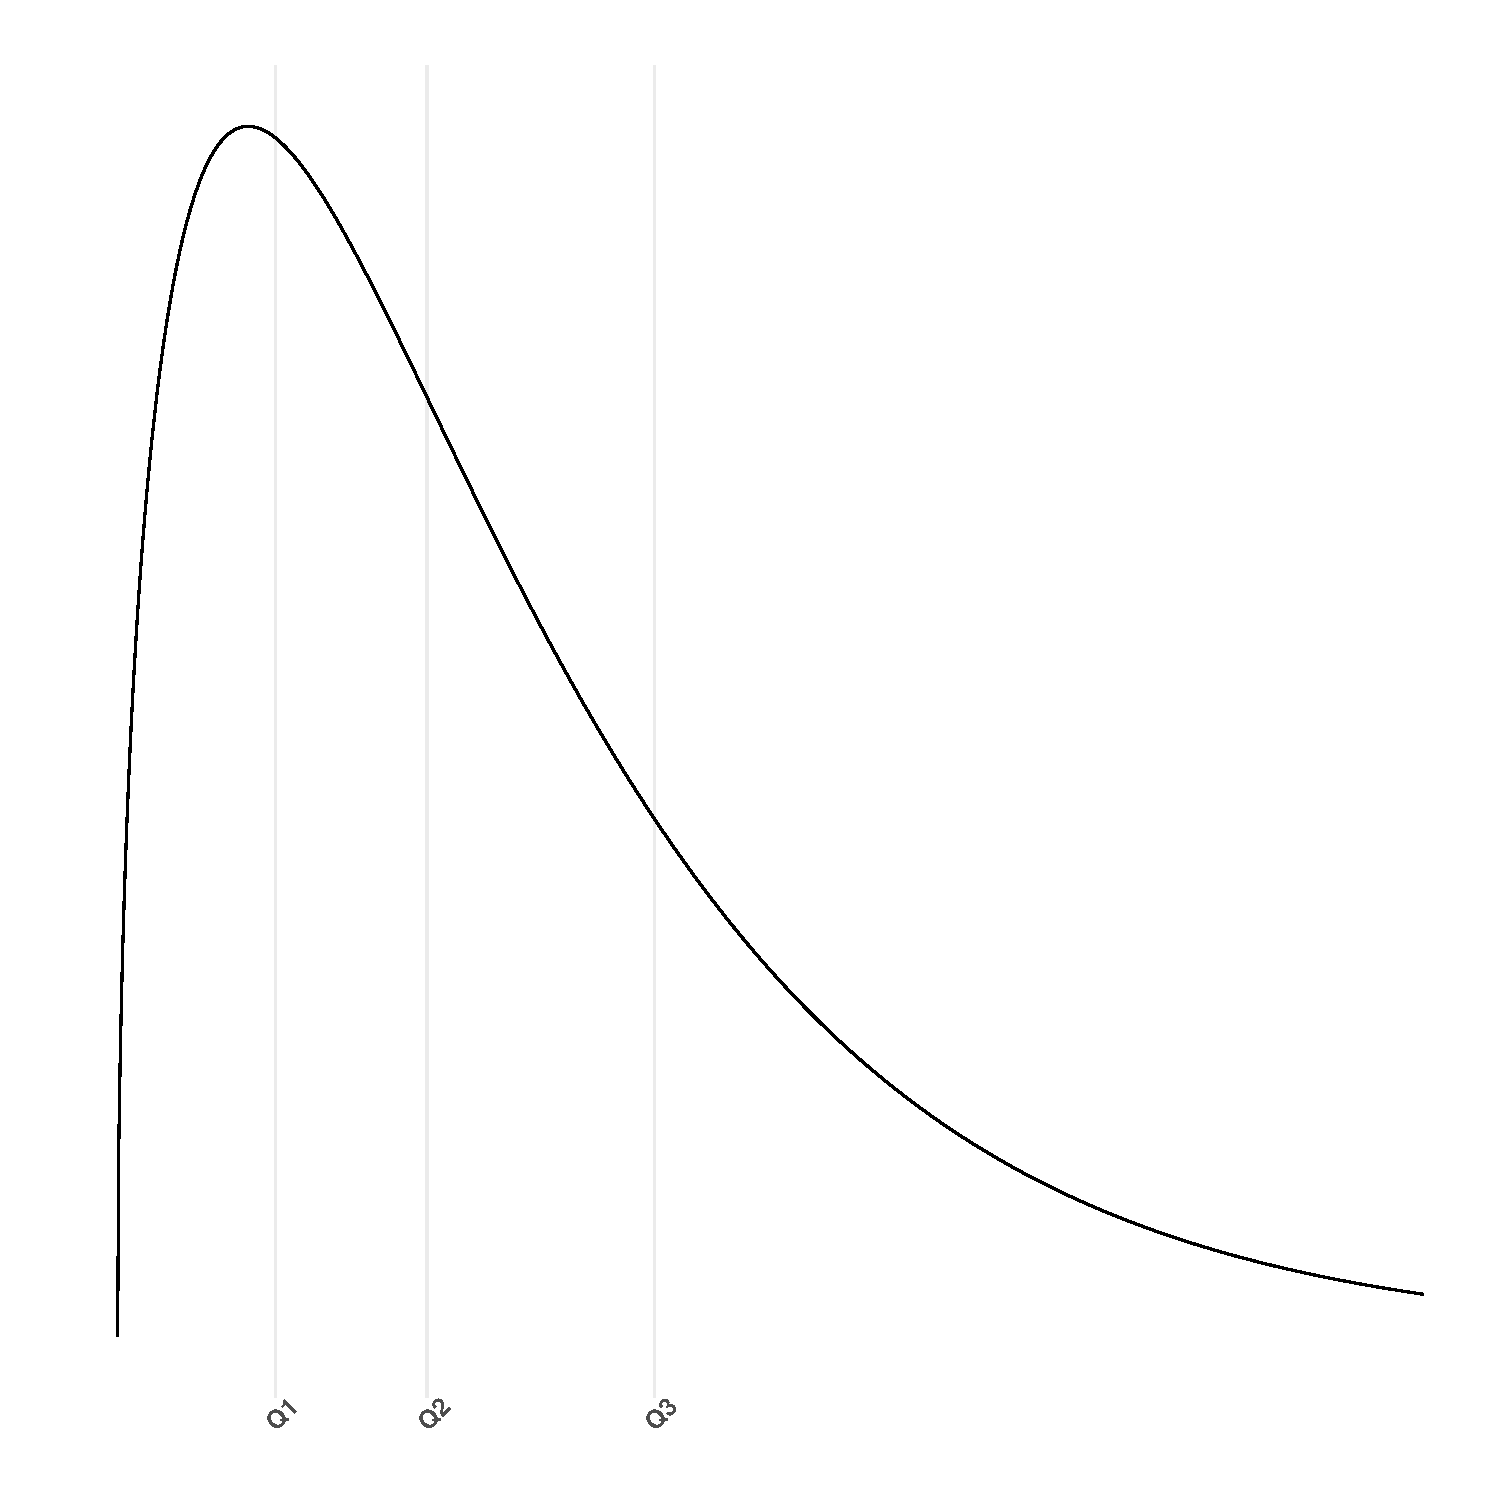
\includegraphics{bookdown_files/figure-latex/unnamed-chunk-108-1.pdf}

\hypertarget{desvio-estandar}{%
\subsubsection{Desvío estándar}\label{desvio-estandar}}

\begin{itemize}
\tightlist
\item
  El \emph{desvío estándar} es una medida de dispersión de los datos, que indica cuánto se suelen alejar de la media.
\end{itemize}

\hypertarget{graficos-estadisticos}{%
\subsection{Gráficos estadísticos}\label{graficos-estadisticos}}

Cerramos la explicación con algunos gráficos que resultan útiles para entender las propiedades estadísticas de los datos.

\hypertarget{boxplot}{%
\subsubsection{Boxplot}\label{boxplot}}

El Boxplot es muy útil para describir una distribución y para detectar outliers. Reúne los principales valores que caracterizan a una distribución:

\begin{itemize}
\tightlist
\item
  \(Q_1\)
\item
  \(Q_2\) (la mediana)
\item
  \(Q_3\)
\item
  el \emph{rango intercuarítlico} \(Q_3 - Q_1\), que define el centro de la distribución
\item
  Outliers, definidos como aquellos puntos que se encuentran a más de 1,5 veces el rango intercuartílico del centro de la distribución.
\end{itemize}

Veamos qué pinta tienen los boxplot de números generados aleatoriamente a partir de tres distribuciones que ya vimos. En este caso, sólo tomaremos 15 valores de cada distribución

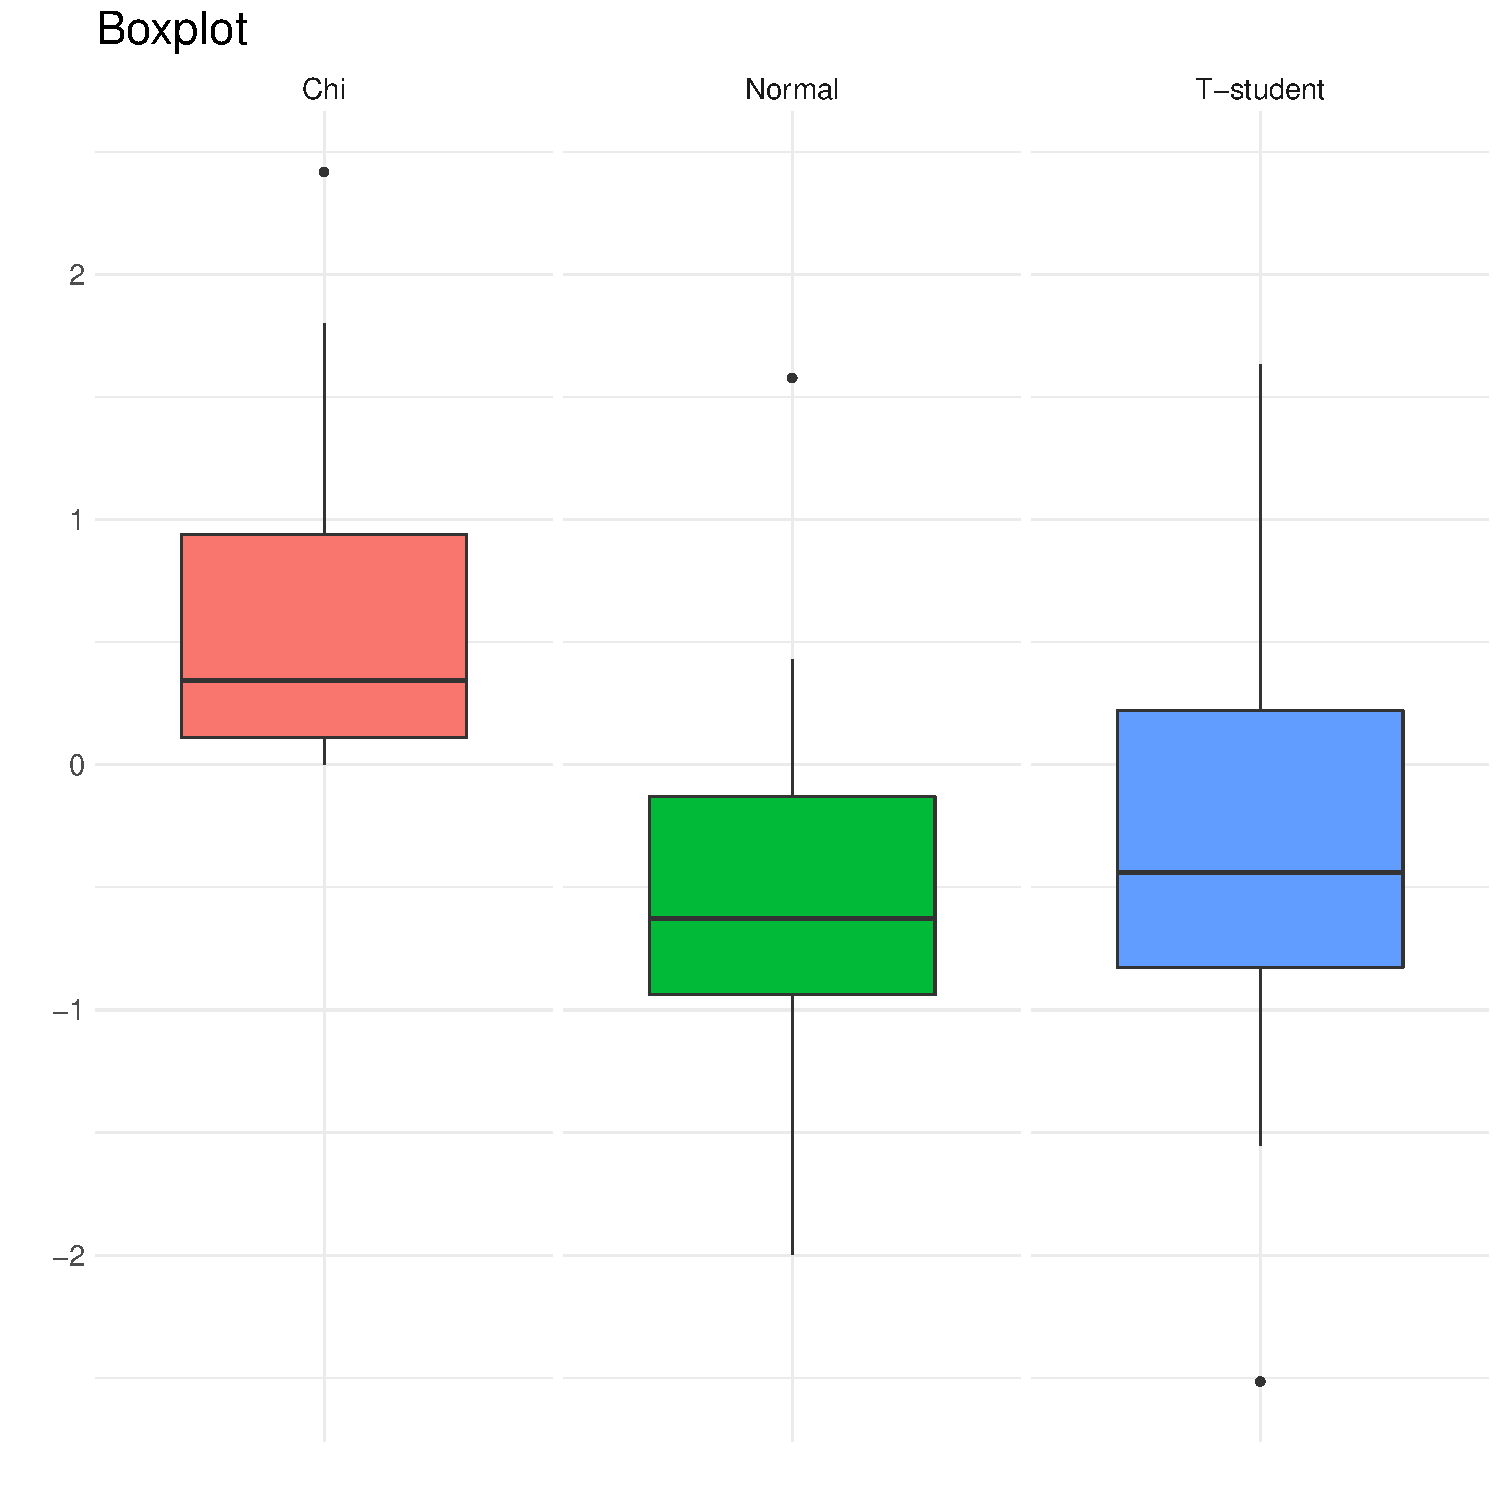
\includegraphics{bookdown_files/figure-latex/unnamed-chunk-109-1.pdf}

Algunas cosas que resaltan:

\begin{itemize}
\tightlist
\item
  la distribución \(\chi^2\) no toma valores en los negativos.
\item
  La normal esta más concentrada en el centro de la distribución.
\end{itemize}

Podemos generar 100 números aleatorios en lugar de 15:

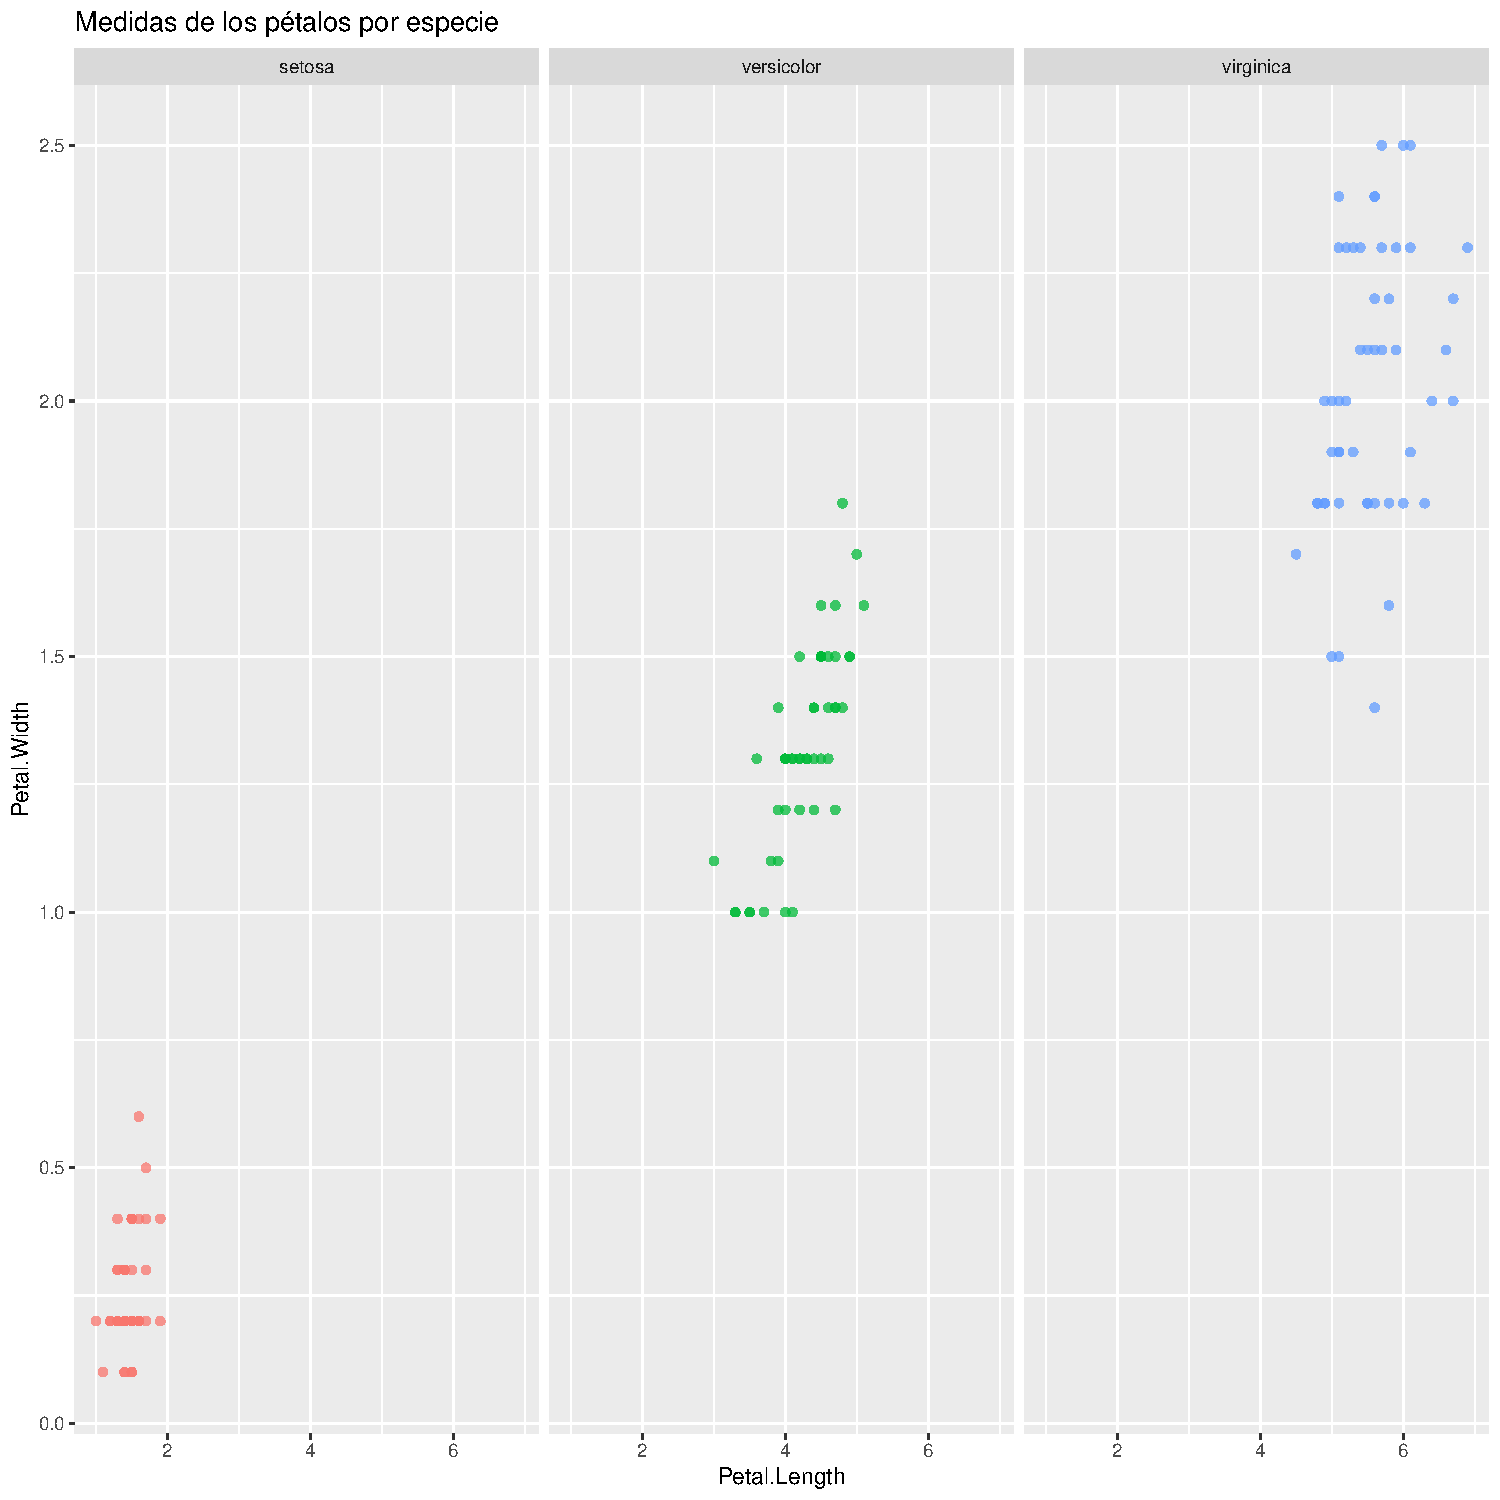
\includegraphics{bookdown_files/figure-latex/unnamed-chunk-110-1.pdf}

Cuando generamos 100 valores en lugar de 15, tenemos más chances de agarrar un punto alejado en la distribución. De esta forma podemos apreciar las diferencias entre la distribución normal y la T-student.

También podemos volver a repasar qué efecto generan los distintos parámetros. Por ejemplo:

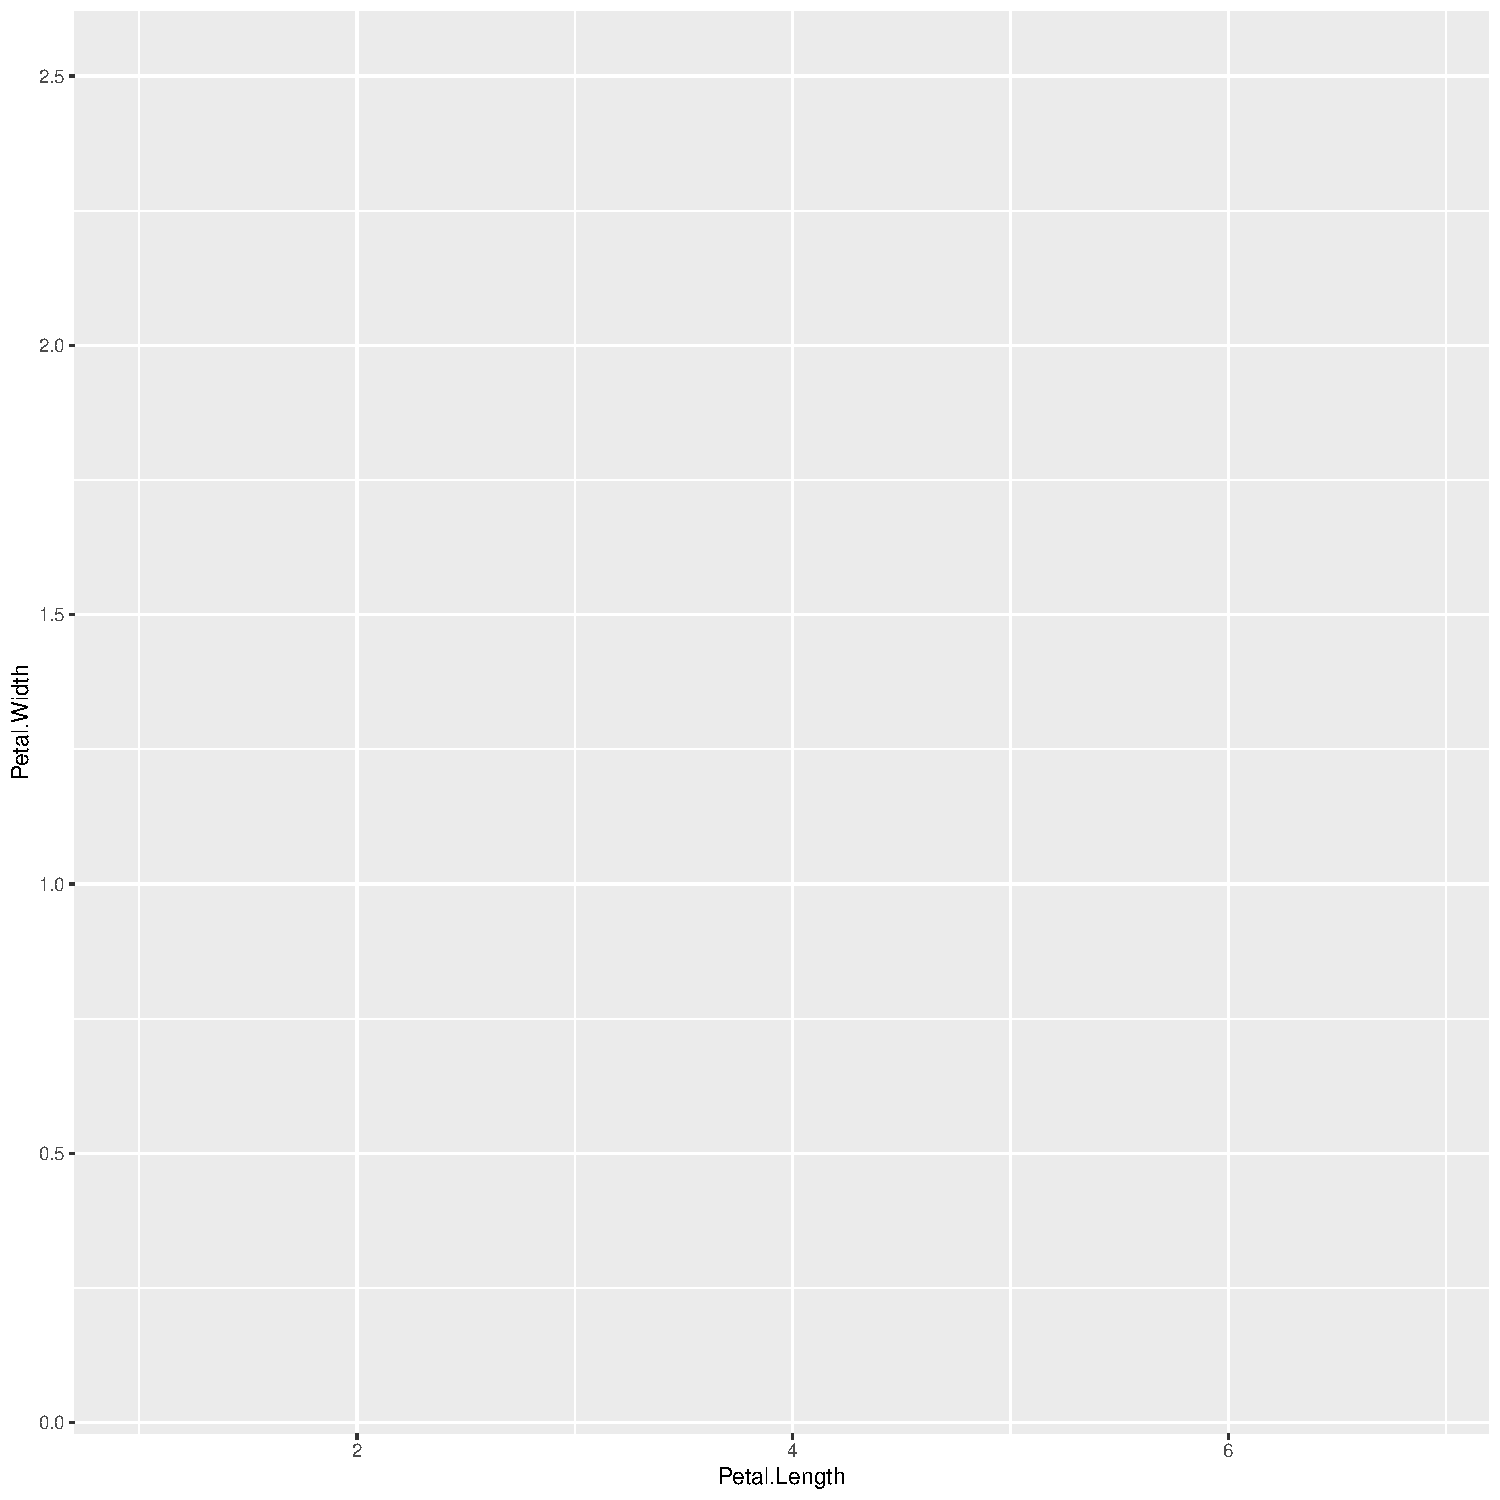
\includegraphics{bookdown_files/figure-latex/unnamed-chunk-111-1.pdf}

\hypertarget{histograma}{%
\subsubsection{Histograma}\label{histograma}}

Otra forma de analizar una distribución es mediante los histogramas:

\begin{itemize}
\tightlist
\item
  En un histograma agrupamos las observaciones en rangos fijos de la variable y contamos la cantidad de ocurrencias.
\item
  Cuanto más alta es una barra, es porque más observaciones se encuentran en dicho rango.
\end{itemize}

Veamos el mismo ejemplo que arriba, pero con histogramas:

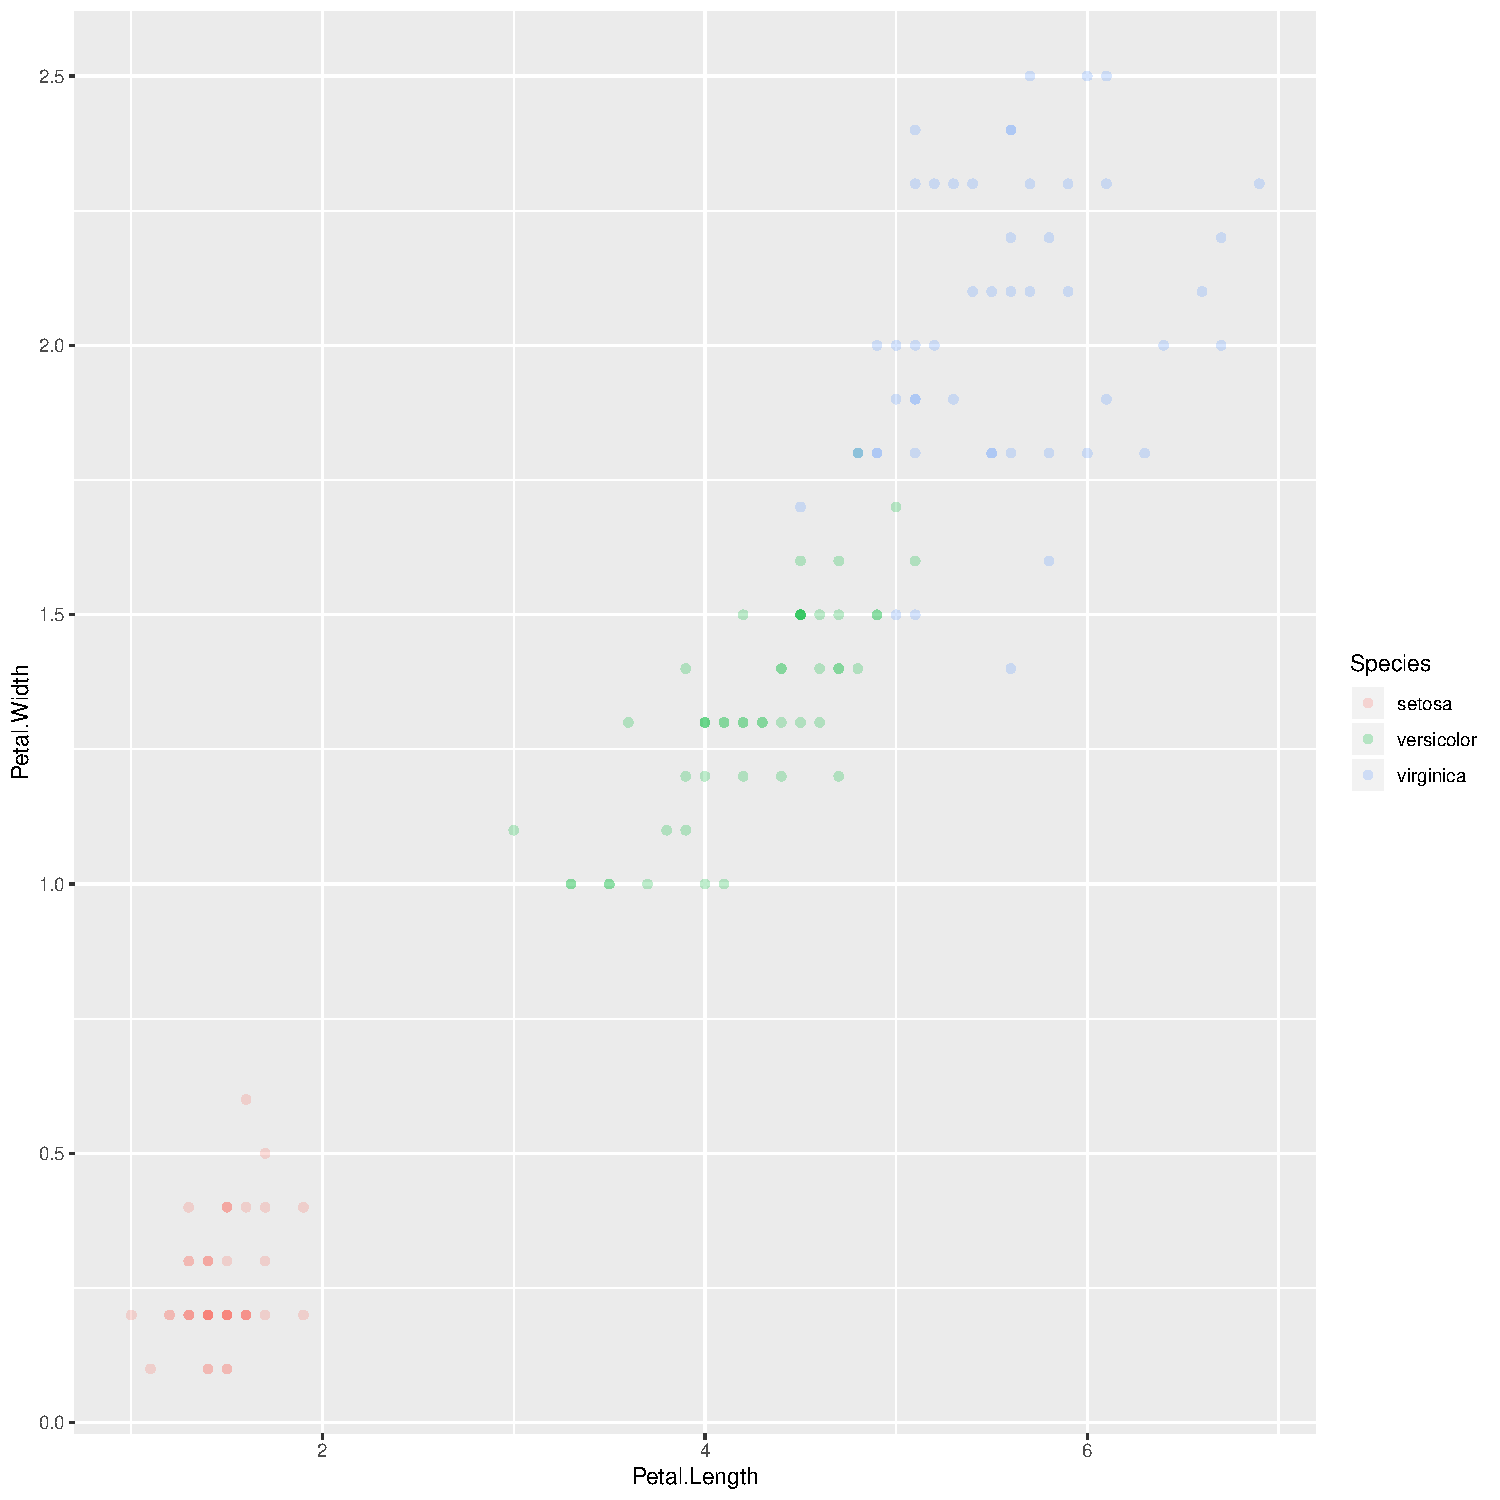
\includegraphics{bookdown_files/figure-latex/unnamed-chunk-112-1.pdf} 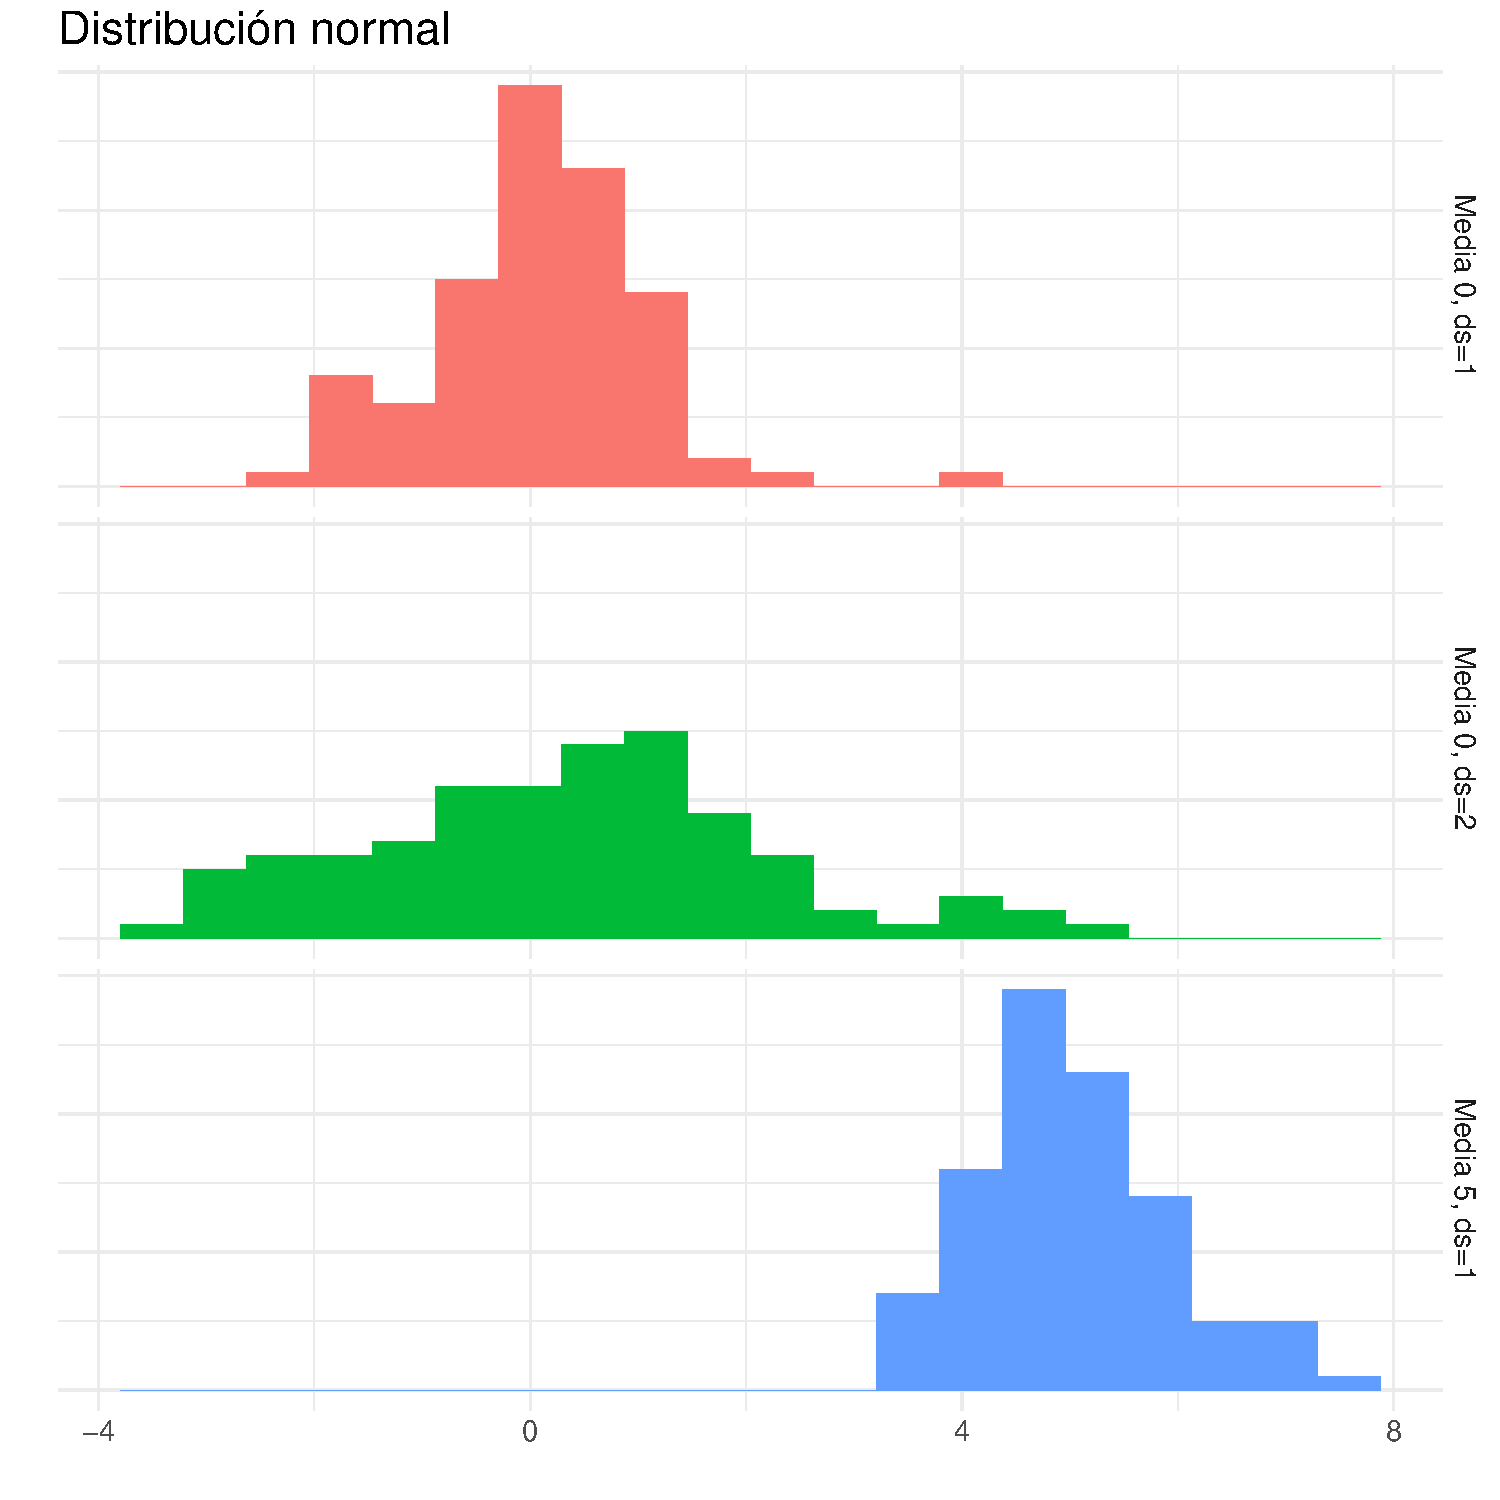
\includegraphics{bookdown_files/figure-latex/unnamed-chunk-112-2.pdf}

\hypertarget{kernel}{%
\subsubsection{Kernel}\label{kernel}}

Los Kernels son simplemente un suavizado sobre los histogramas.

\includegraphics{bookdown_files/figure-latex/unnamed-chunk-113-1.pdf} \includegraphics{bookdown_files/figure-latex/unnamed-chunk-113-2.pdf}

\hypertarget{violin-plots}{%
\subsubsection{Violin plots}\label{violin-plots}}

Combinando la idea de Kernels y Boxplots, se crearon los violin plots, que simplemente muestran a los kernels duplicados.

\includegraphics{bookdown_files/figure-latex/unnamed-chunk-114-1.pdf} \includegraphics{bookdown_files/figure-latex/unnamed-chunk-114-2.pdf}

\hypertarget{bibliografia-de-consulta-1}{%
\subsection{Bibliografía de consulta}\label{bibliografia-de-consulta-1}}

Quién quiera profundizar en estos temas, puede ver los siguientes materiales:

\begin{itemize}
\tightlist
\item
  \url{https://seeing-theory.brown.edu/}
\item
  \url{https://lagunita.stanford.edu/courses/course-v1:OLI+ProbStat+Open_Jan2017/about}
\item
  Jay L. Devore, ``Probabilidad y Estadística para Ingeniería y Ciencias'', International Thomson Editores. \url{https://inferencialitm.files.wordpress.com/2018/04/probabilidad-y-estadistica-para-ingenieria-y-ciencias-devore-7th.pdf}
\end{itemize}

\hypertarget{practica-guiada-4}{%
\section{Práctica Guiada}\label{practica-guiada-4}}

\begin{Shaded}
\begin{Highlighting}[]
\KeywordTok{library}\NormalTok{(tidyverse)}
\end{Highlighting}
\end{Shaded}

\hypertarget{generacion-de-datos-aleatorios}{%
\subsection{Generación de datos aleatorios}\label{generacion-de-datos-aleatorios}}

Para generar datos aleatorios, usamos las funciones:

\begin{itemize}
\tightlist
\item
  \texttt{rnorm} para generar datos que surgen de una distribución normal
\item
  \texttt{rt} para generar datos que surgen de una distribución T-student
\item
  \texttt{rchisq} para generar datos que surgen de una distribución Chi cuadrado
\end{itemize}

\begin{quote}
Pero antes, tenemos que fijar la \emph{semilla} para que los datos sean reproducibles
\end{quote}

\begin{Shaded}
\begin{Highlighting}[]
\KeywordTok{set.seed}\NormalTok{(}\DecValTok{1234}\NormalTok{)}
\KeywordTok{rnorm}\NormalTok{(}\DataTypeTok{n =} \DecValTok{15}\NormalTok{, }\DataTypeTok{mean =} \DecValTok{0}\NormalTok{, }\DataTypeTok{sd =} \DecValTok{1}\NormalTok{ )}
\end{Highlighting}
\end{Shaded}

\begin{verbatim}
##  [1] -1.20706575  0.27742924  1.08444118 -2.34569770  0.42912469
##  [6]  0.50605589 -0.57473996 -0.54663186 -0.56445200 -0.89003783
## [11] -0.47719270 -0.99838644 -0.77625389  0.06445882  0.95949406
\end{verbatim}

\begin{Shaded}
\begin{Highlighting}[]
\KeywordTok{rt}\NormalTok{(}\DataTypeTok{n =} \DecValTok{15}\NormalTok{, }\DataTypeTok{df=}\DecValTok{1}\NormalTok{ )}
\end{Highlighting}
\end{Shaded}

\begin{verbatim}
##  [1] -0.363717710 -1.603466805 -0.388596796 -0.588007490  0.007839245
##  [6] 14.690527710 -1.863488555  0.022667470 -2.084247299 -0.249237745
## [11] -1.311594174 -3.569055208 -2.490838240 -3.848779244 -4.271087169
\end{verbatim}

\begin{Shaded}
\begin{Highlighting}[]
\KeywordTok{rchisq}\NormalTok{(}\DataTypeTok{n =} \DecValTok{15}\NormalTok{,}\DataTypeTok{df=}\DecValTok{1}\NormalTok{)}
\end{Highlighting}
\end{Shaded}

\begin{verbatim}
##  [1] 0.5317744 1.4263809 4.2797098 0.2184660 0.6923773 0.0455256 3.1902100
##  [8] 0.2949942 0.5403827 0.1543732 0.8639196 0.1417290 1.1386091 0.2966193
## [15] 0.5110879
\end{verbatim}

Para poder ver rápidamente de qué se tratan los valores, podemos usar el comando \texttt{plot}

\begin{Shaded}
\begin{Highlighting}[]
\KeywordTok{plot}\NormalTok{(}\KeywordTok{rnorm}\NormalTok{(}\DataTypeTok{n =} \DecValTok{15}\NormalTok{,}\DataTypeTok{mean =} \DecValTok{0}\NormalTok{, }\DataTypeTok{sd =} \DecValTok{1}\NormalTok{ ))}
\end{Highlighting}
\end{Shaded}

\includegraphics{bookdown_files/figure-latex/unnamed-chunk-118-1.pdf}

\begin{Shaded}
\begin{Highlighting}[]
\KeywordTok{plot}\NormalTok{(}\KeywordTok{rt}\NormalTok{(}\DataTypeTok{n =} \DecValTok{15}\NormalTok{,}\DataTypeTok{df=}\DecValTok{1}\NormalTok{ ))}
\end{Highlighting}
\end{Shaded}

\includegraphics{bookdown_files/figure-latex/unnamed-chunk-118-2.pdf}

\begin{Shaded}
\begin{Highlighting}[]
\KeywordTok{plot}\NormalTok{(}\KeywordTok{rchisq}\NormalTok{(}\DataTypeTok{n =} \DecValTok{15}\NormalTok{,}\DataTypeTok{df=}\DecValTok{1}\NormalTok{))}
\end{Highlighting}
\end{Shaded}

\includegraphics{bookdown_files/figure-latex/unnamed-chunk-118-3.pdf}

Noten que el eje X es el índice de los valores, es decir que no agrega información.

\hypertarget{tests}{%
\subsection{Tests}\label{tests}}

Utilicemos ahora datos reales.

Los datos salen de \url{https://data.buenosaires.gob.ar/dataset/femicidios}

\begin{quote}
Vamos a ver ahora las estadisticas de Buenos Aires sobre la cantidad de femicidios por grupo etario. Es interesante preguntarse si hay más femicidios para cierto rango etario.
\end{quote}

\begin{Shaded}
\begin{Highlighting}[]
\NormalTok{femicidios <-}\StringTok{ }\KeywordTok{read_csv}\NormalTok{(}\DataTypeTok{file =} \StringTok{'fuentes/vict_fem_annio__g_edad_limpio.csv'}\NormalTok{)}
\NormalTok{femicidios}
\end{Highlighting}
\end{Shaded}

\begin{verbatim}
## # A tibble: 19 x 3
##     anio cantidad_femicidios grupo_edad
##    <dbl> <chr>               <chr>     
##  1  2015 1                   0 - 15    
##  2  2015 2                   16 - 20   
##  3  2015 5                   21 - 40   
##  4  2015 3                   41 - 60   
##  5  2015 -                   61 y más  
##  6  2015 1                   Ignorado  
##  7  2016 2                   0 - 15    
##  8  2016 3                   16 - 20   
##  9  2016 4                   21 - 40   
## 10  2016 1                   41 - 60   
## 11  2016 2                   61 y más  
## 12  2016 2                   Ignorado  
## 13  2017 …                   0 - 15    
## 14  2017 …                   16 - 20   
## 15  2017 …                   21 - 40   
## 16  2017 …                   41 - 60   
## 17  2017 …                   61 y más  
## 18  2017 …                   Ignorado  
## 19  2017 9                   TOTAL
\end{verbatim}

Fijense que las estadísitcas no están desagregadas por rango etario para 2017, que en caso de que haya 0 femicidios pusieron `-' en lugar de 0. Además, como tenemos pocos datos, es mejor hacer un test que compare sólamente dos grupos.

Vamos a reorganizar la información para corregir todas estas cosas

\begin{Shaded}
\begin{Highlighting}[]
\NormalTok{femicidios <-}\StringTok{ }\NormalTok{femicidios }\OperatorTok\StringTok{ }
\StringTok{  }\KeywordTok{filter}\NormalTok{(anio}\OperatorTok{!=}\DecValTok{2017}\NormalTok{, grupo_edad }\OperatorTok{!=}\StringTok{'Ignorado'}\NormalTok{) }\OperatorTok\StringTok{  }\CommentTok{#Sacamos al 2017 y los casos donde se ignora la edad}
\StringTok{  }\KeywordTok{mutate}\NormalTok{(}\DataTypeTok{cantidad_femicidios =} \KeywordTok{case_when}\NormalTok{(cantidad_femicidios}\OperatorTok{==}\StringTok{'-'} \OperatorTok{~}\StringTok{ }\DecValTok{0}\NormalTok{, }\CommentTok{# reemplazamos el - por 0}
                                         \OtherTok{TRUE} \OperatorTok{~}\KeywordTok{as.numeric}\NormalTok{(cantidad_femicidios)), }\CommentTok{# y convertimos la variable en numerica}
         \DataTypeTok{grupo_edad =} \KeywordTok{case_when}\NormalTok{(grupo_edad }\OperatorTok\StringTok{ }\KeywordTok{c}\NormalTok{(}\StringTok{'0 - 15'}\NormalTok{,}\StringTok{'16 - 20'}\NormalTok{,}\StringTok{'21 - 40'}\NormalTok{) }\OperatorTok{~}\StringTok{ '0-40'}\NormalTok{, }\CommentTok{# agrupamos para tener sólo dos grupos}
\NormalTok{                                grupo_edad }\OperatorTok\StringTok{ }\KeywordTok{c}\NormalTok{(}\StringTok{'41 - 60'}\NormalTok{,}\StringTok{'61 y más'}\NormalTok{) }\OperatorTok{~}\StringTok{ '41 y más'}\NormalTok{)) }\OperatorTok\StringTok{ }
\StringTok{  }\KeywordTok{group_by}\NormalTok{(grupo_edad) }\OperatorTok\StringTok{ }
\StringTok{  }\KeywordTok{summarise}\NormalTok{(}\DataTypeTok{cantidad_femicidios=} \KeywordTok{sum}\NormalTok{(cantidad_femicidios)) }\CommentTok{# sumamos los años y grupos para tener datos agregados}
\NormalTok{femicidios}
\end{Highlighting}
\end{Shaded}

\begin{verbatim}
## # A tibble: 2 x 2
##   grupo_edad cantidad_femicidios
##   <chr>                    <dbl>
## 1 0-40                        17
## 2 41 y más                     6
\end{verbatim}

Con esta tabla de contingencia podemos hacer un test de hipótesis.

¿Cuál usamos? Nos fijamos en el machete, o googleamos, y vemos que como queremos comparar la cantidad de casos por grupos categóricos, tenemos que usar el test Chi.

\begin{itemize}
\tightlist
\item
  \(H_0\) No hay asociación entre las variables
\item
  \(H_1\) Hay asociación entre las variables
\end{itemize}

La idea es que tenemos dos variables: El rango etario y la cantidad de femicidios

\begin{Shaded}
\begin{Highlighting}[]
\KeywordTok{chisq.test}\NormalTok{(femicidios}\OperatorTok{$}\NormalTok{cantidad_femicidios)}
\end{Highlighting}
\end{Shaded}

\begin{verbatim}
## 
##  Chi-squared test for given probabilities
## 
## data:  femicidios$cantidad_femicidios
## X-squared = 5.2609, df = 1, p-value = 0.02181
\end{verbatim}

Noten que el resultado lo dan en términos del p-valor. Como el valor es bajo, menor a 0.05, entonces podemos rechazar que no existe relación. O en otros términos, pareciera que la diferencia es significativa estadísticamente.

\hypertarget{descripcion-estadistica-de-los-datos}{%
\subsection{Descripción estadística de los datos}\label{descripcion-estadistica-de-los-datos}}

Volveremos a ver los datos de \href{https://data.buenosaires.gob.ar/dataset/sueldo-funcionarios}{sueldos de funcionarios}

\begin{Shaded}
\begin{Highlighting}[]
\NormalTok{sueldos <-}\StringTok{ }\KeywordTok{read_csv}\NormalTok{(}\StringTok{'fuentes/sueldo_funcionarios_2019.csv'}\NormalTok{)}
\end{Highlighting}
\end{Shaded}

Con el comando \texttt{summary} podemos ver algunos de los principales estadísticos de resumen

\begin{Shaded}
\begin{Highlighting}[]
\KeywordTok{summary}\NormalTok{(sueldos}\OperatorTok{$}\NormalTok{asignacion_por_cargo_i)}
\end{Highlighting}
\end{Shaded}

\begin{verbatim}
##    Min. 1st Qu.  Median    Mean 3rd Qu.    Max. 
##  197746  210061  226866  225401  231168  249662
\end{verbatim}

\hypertarget{graficos-estadisticos-1}{%
\subsection{Gráficos estadísticos}\label{graficos-estadisticos-1}}

No nos vamos a detener demasiado a ver cómo hacer los gráficos de resumen, porque la próxima clase veremos como realizar gráficos de mejor calidad, como los presentados en las notas de clase.

A modo de ejemplo, dejamos los comandos de R base para realizar gráficos.

\begin{Shaded}
\begin{Highlighting}[]
\KeywordTok{boxplot}\NormalTok{(sueldos}\OperatorTok{$}\NormalTok{asignacion_por_cargo_i)}
\end{Highlighting}
\end{Shaded}

\includegraphics{bookdown_files/figure-latex/unnamed-chunk-124-1.pdf}

\begin{Shaded}
\begin{Highlighting}[]
\KeywordTok{hist}\NormalTok{(sueldos}\OperatorTok{$}\NormalTok{asignacion_por_cargo_i)}
\end{Highlighting}
\end{Shaded}

\includegraphics{bookdown_files/figure-latex/unnamed-chunk-124-2.pdf}

\begin{Shaded}
\begin{Highlighting}[]
\KeywordTok{plot}\NormalTok{(}\KeywordTok{density}\NormalTok{(sueldos}\OperatorTok{$}\NormalTok{asignacion_por_cargo_i))}
\end{Highlighting}
\end{Shaded}

\includegraphics{bookdown_files/figure-latex/unnamed-chunk-124-3.pdf}

\hypertarget{modelo-lineal}{%
\chapter{Modelo Lineal}\label{modelo-lineal}}

\hypertarget{explicacion-5}{%
\section{Explicación}\label{explicacion-5}}

En este módulo vamos a ver cómo analizar la relación entre dos variables. Primero, veremos los conceptos de covarianza y correlación, y luego avanzaremos hasta el modelo lineal.

\begin{Shaded}
\begin{Highlighting}[]
\NormalTok{knitr}\OperatorTok{::}\NormalTok{opts_chunk}\OperatorTok{$}\KeywordTok{set}\NormalTok{(}\DataTypeTok{warning =} \OtherTok{FALSE}\NormalTok{, }\DataTypeTok{message =} \OtherTok{FALSE}\NormalTok{)}
\KeywordTok{library}\NormalTok{(tidyverse)}
\KeywordTok{library}\NormalTok{(modelr)}
\KeywordTok{library}\NormalTok{(GGally)}
\KeywordTok{library}\NormalTok{(plot3D)}
\end{Highlighting}
\end{Shaded}

\hypertarget{covarianza-y-correlacion.}{%
\subsection{Covarianza y Correlación.}\label{covarianza-y-correlacion.}}

La covarianza mide cómo varían de forma conjunta dos variables, en promedio. Se define como:

\[
\text{cov}(x,y)=\frac{1}{n}\sum_{i=1}^n(x_i-\bar x)(y_i-\bar y)
\]

Esto es: La covarianza entre dos variables, \(x\) e \(y\) es el promedio (noten que hay una sumatoria y un dividido n) de las diferencias de los puntos a sus medias en \(x\) e \(y\).

tratemos de entender el trabalenguas con la ayuda del siguiente gráfico:

\includegraphics{bookdown_files/figure-latex/unnamed-chunk-125-1.pdf}

Aquí marcamos \(\bar x\) y \(\bar y\) y dividimos el gráfico en cuatro cuadrantes.

\begin{enumerate}
\def\labelenumi{\arabic{enumi}.}
\tightlist
\item
  En el primer cuadrante los puntos son más chicos a sus medias en \(x\) y en \(y\), \((x-\hat x)\) es negativo y \((y-\hat y)\) también. Por lo tanto, su producto es positivo.
\item
  En el segundo cuadrante la diferencia es negativa en x, pero positiva en y. Por lo tanto el producto es negativo.
\item
  En el tercer cuadrante la diferencia es negativa en y, pero positiva en x. Por lo tanto el producto es negativo.
\item
  Finalmente, en el cuarto cuadrante las diferencias son positivas tanto en x como en y, y por lo tanto también el producto.
\end{enumerate}

\begin{itemize}
\tightlist
\item
  Si la covarianza es \textbf{positiva} y grande, entonces valores chicos en una de las variables suceden en conjunto con valores chicos en la otra,y viceversa.
\item
  Al contrario, si la covarianza es \textbf{negativa} y grande, entonces valores altos de una variable suceden en conjunto con valores pequeños de la otra y viceversa.
\end{itemize}

La correlación se define como sigue:

\[\rho_{x,y}=\frac{cov(x,y)}{\sigma_x \sigma_y}\]

Es decir, normalizamos la covarianza por el desvío en \(x\) y en \(y\). de esta forma, la correlación se define entre -1 y 1.

\hypertarget{ggpairs}{%
\subsubsection{ggpairs}\label{ggpairs}}

Para ver una implementación práctica de estos conceptos, vamos a utilizar la librería \href{https://ggobi.github.io/ggally/}{\emph{GGally}} para graficar la correlación por pares de variables.

\begin{itemize}
\tightlist
\item
  Con \texttt{ggpairs()}, podemos graficar todas las variables, y buscar las correlaciones. Coloreamos por:
\end{itemize}

-\(am\): Tipo de transmisión: automático (am=0) o manual (am=1)

\begin{Shaded}
\begin{Highlighting}[]
\NormalTok{mtcars }\OperatorTok\StringTok{ }
\StringTok{  }\KeywordTok{select}\NormalTok{(}\OperatorTok{-}\NormalTok{carb,}\OperatorTok{-}\NormalTok{vs) }\OperatorTok\StringTok{ }
\StringTok{  }\KeywordTok{mutate}\NormalTok{(}\DataTypeTok{cyl =} \KeywordTok{factor}\NormalTok{(cyl),}
         \DataTypeTok{am =} \KeywordTok{factor}\NormalTok{(am)) }\OperatorTok\StringTok{ }
\KeywordTok{ggpairs}\NormalTok{(., }
        \DataTypeTok{title =} \StringTok{"Matriz de correlaciones"}\NormalTok{,}
        \DataTypeTok{mapping =} \KeywordTok{aes}\NormalTok{(}\DataTypeTok{colour=}\NormalTok{ am))}
\end{Highlighting}
\end{Shaded}

\includegraphics{bookdown_files/figure-latex/unnamed-chunk-126-1.pdf}

Veamos la correlación entre:

\begin{itemize}
\tightlist
\item
  \(mpg\): Miles/(US) gallon. Eficiencia de combustible
\item
  \(hp\): Gross horsepower: Potencia del motor
\end{itemize}

\begin{Shaded}
\begin{Highlighting}[]
\KeywordTok{cor}\NormalTok{(mtcars}\OperatorTok{$}\NormalTok{mpg, mtcars}\OperatorTok{$}\NormalTok{hp)}
\end{Highlighting}
\end{Shaded}

\begin{verbatim}
## [1] -0.7761684
\end{verbatim}

nos da negativa y alta.

\begin{itemize}
\tightlist
\item
  Si quisiéramos testear la significatividad de este estimador, podemos realizar un test:
\end{itemize}

\(H_0\) : ρ =0\\
\(H_1\) : ρ \(\neq\) 0

\begin{Shaded}
\begin{Highlighting}[]
\KeywordTok{cor.test}\NormalTok{(mtcars}\OperatorTok{$}\NormalTok{mpg,mtcars}\OperatorTok{$}\NormalTok{hp)}
\end{Highlighting}
\end{Shaded}

\begin{verbatim}
## 
##  Pearson's product-moment correlation
## 
## data:  mtcars$mpg and mtcars$hp
## t = -6.7424, df = 30, p-value = 1.788e-07
## alternative hypothesis: true correlation is not equal to 0
## 95 percent confidence interval:
##  -0.8852686 -0.5860994
## sample estimates:
##        cor 
## -0.7761684
\end{verbatim}

Con este p-value rechazamos \(H_0\)

\hypertarget{modelo-lineal-1}{%
\subsection{Modelo Lineal}\label{modelo-lineal-1}}

sigamos utilizando los datos de \emph{sim1}

\begin{Shaded}
\begin{Highlighting}[]
\KeywordTok{ggplot}\NormalTok{(sim1, }\KeywordTok{aes}\NormalTok{(x, y)) }\OperatorTok{+}\StringTok{ }
\StringTok{  }\KeywordTok{geom_point}\NormalTok{()}
\end{Highlighting}
\end{Shaded}

\includegraphics{bookdown_files/figure-latex/unnamed-chunk-129-1.pdf}

Se puede ver un patrón fuerte en los datos. Pareciera que el modelo lineal \texttt{y\ =\ a\_0\ +\ a\_1\ *\ x} podría servir.

\hypertarget{modelos-al-azar}{%
\subsubsection{Modelos al azar}\label{modelos-al-azar}}

Para empezar, generemos aleatoriamente varios modelos lineales para ver qué pinta tienen. Para eso, podemos usar \texttt{geom\_abline\ ()} que toma una pendiente e intercepto como parámetros.

\begin{Shaded}
\begin{Highlighting}[]
\NormalTok{models <-}\StringTok{ }\KeywordTok{tibble}\NormalTok{(}
  \DataTypeTok{a1 =} \KeywordTok{runif}\NormalTok{(}\DecValTok{250}\NormalTok{, }\DecValTok{-20}\NormalTok{, }\DecValTok{40}\NormalTok{),}
  \DataTypeTok{a2 =} \KeywordTok{runif}\NormalTok{(}\DecValTok{250}\NormalTok{, }\DecValTok{-5}\NormalTok{, }\DecValTok{5}\NormalTok{)}
\NormalTok{)}

\KeywordTok{ggplot}\NormalTok{(sim1, }\KeywordTok{aes}\NormalTok{(x, y)) }\OperatorTok{+}\StringTok{ }
\StringTok{  }\KeywordTok{geom_abline}\NormalTok{(}\KeywordTok{aes}\NormalTok{(}\DataTypeTok{intercept =}\NormalTok{ a1, }\DataTypeTok{slope =}\NormalTok{ a2), }\DataTypeTok{data =}\NormalTok{ models, }\DataTypeTok{alpha =} \DecValTok{1}\OperatorTok{/}\DecValTok{4}\NormalTok{) }\OperatorTok{+}
\StringTok{  }\KeywordTok{geom_point}\NormalTok{() }
\end{Highlighting}
\end{Shaded}

\includegraphics{bookdown_files/figure-latex/unnamed-chunk-130-1.pdf}

A simple vista podemos apreciar que algunos modelos son mejores que otros. Pero necesitamos una forma de cuantificar cuales son los \emph{mejores} modelos.

\hypertarget{distancias}{%
\subsubsection{distancias}\label{distancias}}

Una forma de definir \emph{mejor} es pensar en aquel modelo que minimiza la distancia vertical con cada punto:

Para eso, eligamos un modelo cualquiera:

\[ y= 7 + 1.5*x\]

(para que se vean mejor las distancias, corremos un poquito cada punto sobre el eje x)

\begin{Shaded}
\begin{Highlighting}[]
\NormalTok{dist1 <-}\StringTok{ }\NormalTok{sim1 }\OperatorTok\StringTok{ }
\StringTok{  }\KeywordTok{mutate}\NormalTok{(}
    \DataTypeTok{dodge =} \KeywordTok{rep}\NormalTok{(}\KeywordTok{c}\NormalTok{(}\OperatorTok{-}\DecValTok{1}\NormalTok{, }\DecValTok{0}\NormalTok{, }\DecValTok{1}\NormalTok{) }\OperatorTok{/}\StringTok{ }\DecValTok{20}\NormalTok{, }\DecValTok{10}\NormalTok{),}
    \DataTypeTok{x1 =}\NormalTok{ x }\OperatorTok{+}\StringTok{ }\NormalTok{dodge,}
    \DataTypeTok{pred =} \DecValTok{7} \OperatorTok{+}\StringTok{ }\NormalTok{x1 }\OperatorTok{*}\StringTok{ }\FloatTok{1.5}
\NormalTok{  )}

\KeywordTok{ggplot}\NormalTok{(dist1, }\KeywordTok{aes}\NormalTok{(x1, y)) }\OperatorTok{+}\StringTok{ }
\StringTok{  }\KeywordTok{geom_abline}\NormalTok{(}\DataTypeTok{intercept =} \DecValTok{7}\NormalTok{, }\DataTypeTok{slope =} \FloatTok{1.5}\NormalTok{, }\DataTypeTok{colour =} \StringTok{"grey40"}\NormalTok{) }\OperatorTok{+}
\StringTok{  }\KeywordTok{geom_point}\NormalTok{(}\DataTypeTok{colour =} \StringTok{"grey40"}\NormalTok{) }\OperatorTok{+}
\StringTok{  }\KeywordTok{geom_linerange}\NormalTok{(}\KeywordTok{aes}\NormalTok{(}\DataTypeTok{ymin =}\NormalTok{ y, }\DataTypeTok{ymax =}\NormalTok{ pred), }\DataTypeTok{colour =} \StringTok{"#3366FF"}\NormalTok{) }
\end{Highlighting}
\end{Shaded}

\includegraphics{bookdown_files/figure-latex/unnamed-chunk-131-1.pdf}

La distancia de cada punto a la recta es la diferencia entre lo que predice nuestro modelo y el valor real

Para computar la distancia, primero necesitamos una función que represente a nuestro modelo:

Para eso, vamos a crear una función que reciba un vector con los parámetros del modelo, y el set de datos, y genere la predicción:

\begin{Shaded}
\begin{Highlighting}[]
\NormalTok{model1 <-}\StringTok{ }\ControlFlowTok{function}\NormalTok{(a, data) \{}
\NormalTok{  a[}\DecValTok{1}\NormalTok{] }\OperatorTok{+}\StringTok{ }\NormalTok{data}\OperatorTok{$}\NormalTok{x }\OperatorTok{*}\StringTok{ }\NormalTok{a[}\DecValTok{2}\NormalTok{]}
\NormalTok{\}}

\KeywordTok{model1}\NormalTok{(}\KeywordTok{c}\NormalTok{(}\DecValTok{7}\NormalTok{, }\FloatTok{1.5}\NormalTok{), sim1)}
\end{Highlighting}
\end{Shaded}

\begin{verbatim}
##  [1]  8.5  8.5  8.5 10.0 10.0 10.0 11.5 11.5 11.5 13.0 13.0 13.0 14.5 14.5
## [15] 14.5 16.0 16.0 16.0 17.5 17.5 17.5 19.0 19.0 19.0 20.5 20.5 20.5 22.0
## [29] 22.0 22.0
\end{verbatim}

Ahora, necesitamos una forma de calcular los residuos y agruparlos. Esto lo vamos a hacer con el error cuadrático medio

\[ECM = \sqrt\frac{\sum_i^n{(\hat{y_i} - y_i)^2}}{n}\]

\begin{Shaded}
\begin{Highlighting}[]
\NormalTok{measure_distance <-}\StringTok{ }\ControlFlowTok{function}\NormalTok{(mod, data) \{}
\NormalTok{  diff <-}\StringTok{ }\NormalTok{data}\OperatorTok{$}\NormalTok{y }\OperatorTok{-}\StringTok{ }\KeywordTok{model1}\NormalTok{(mod, data)}
  \KeywordTok{sqrt}\NormalTok{(}\KeywordTok{mean}\NormalTok{(diff }\OperatorTok{^}\StringTok{ }\DecValTok{2}\NormalTok{))}
\NormalTok{\}}

\KeywordTok{measure_distance}\NormalTok{(}\KeywordTok{c}\NormalTok{(}\DecValTok{7}\NormalTok{, }\FloatTok{1.5}\NormalTok{), sim1)}
\end{Highlighting}
\end{Shaded}

\begin{verbatim}
## [1] 2.665212
\end{verbatim}

\hypertarget{evaluando-los-modelos-aleatorios}{%
\subsubsection{Evaluando los modelos aleatorios}\label{evaluando-los-modelos-aleatorios}}

Ahora podemos calcular el \textbf{ECM} para todos los modelos del dataframe \emph{models}. Para eso utilizamos el paquete \textbf{purrr}, para ejecutar varias veces la misma función sobre varios elementos.

Tenemos que pasar los valores de a1 y a2 (dos parámetros --\textgreater{} map2), pero como nuestra función toma sólo uno (el vector a), nos armamos una función de ayuda para \emph{wrapear} a1 y a2

\begin{Shaded}
\begin{Highlighting}[]
\NormalTok{sim1_dist <-}\StringTok{ }\ControlFlowTok{function}\NormalTok{(a1, a2) \{}
  \KeywordTok{measure_distance}\NormalTok{(}\KeywordTok{c}\NormalTok{(a1, a2), sim1)}
\NormalTok{\}}

\NormalTok{models <-}\StringTok{ }\NormalTok{models }\OperatorTok\StringTok{ }
\StringTok{  }\KeywordTok{mutate}\NormalTok{(}\DataTypeTok{dist =}\NormalTok{ purrr}\OperatorTok{::}\KeywordTok{map2_dbl}\NormalTok{(a1, a2, sim1_dist))}
\NormalTok{models}
\end{Highlighting}
\end{Shaded}

\begin{verbatim}
## # A tibble: 250 x 3
##        a1     a2  dist
##     <dbl>  <dbl> <dbl>
##  1 -18.3   4.74  11.2 
##  2  35.8   4.51  45.7 
##  3   4.63  1.16   5.59
##  4  37.4   4.65  48.0 
##  5  -3.67  3.78   5.64
##  6  11.0  -3.80  30.5 
##  7  38.7   0.963 28.7 
##  8   2.18 -1.43  23.5 
##  9  -1.37  1.75   7.61
## 10 -17.9   1.38  26.0 
## # ... with 240 more rows
\end{verbatim}

A continuación, superpongamos los 10 mejores modelos a los datos. Coloreamos los modelos por \texttt{-dist}: esta es una manera fácil de asegurarse de que los mejores modelos (es decir, los que tienen la menor distancia) obtengan los colores más brillantes.

\begin{Shaded}
\begin{Highlighting}[]
\KeywordTok{ggplot}\NormalTok{(sim1, }\KeywordTok{aes}\NormalTok{(x, y)) }\OperatorTok{+}\StringTok{ }
\StringTok{  }\KeywordTok{geom_point}\NormalTok{(}\DataTypeTok{size =} \DecValTok{2}\NormalTok{, }\DataTypeTok{colour =} \StringTok{"grey30"}\NormalTok{) }\OperatorTok{+}\StringTok{ }
\StringTok{  }\KeywordTok{geom_abline}\NormalTok{(}
    \KeywordTok{aes}\NormalTok{(}\DataTypeTok{intercept =}\NormalTok{ a1, }\DataTypeTok{slope =}\NormalTok{ a2, }\DataTypeTok{colour =} \OperatorTok{-}\NormalTok{dist), }
    \DataTypeTok{data =} \KeywordTok{filter}\NormalTok{(models, }\KeywordTok{rank}\NormalTok{(dist) }\OperatorTok{<=}\StringTok{ }\DecValTok{10}\NormalTok{)}
\NormalTok{  )}
\end{Highlighting}
\end{Shaded}

\includegraphics{bookdown_files/figure-latex/unnamed-chunk-135-1.pdf}

También podemos pensar en estos modelos como observaciones y visualizar con un gráfico de dispersión de \texttt{a1} vs\texttt{a2}, nuevamente coloreado por \texttt{-dist}. Ya no podemos ver directamente cómo se compara el modelo con los datos, pero podemos ver muchos modelos a la vez. Nuevamente, destacamos los 10 mejores modelos, esta vez dibujando círculos rojos debajo de ellos.

\begin{Shaded}
\begin{Highlighting}[]
\KeywordTok{ggplot}\NormalTok{(models, }\KeywordTok{aes}\NormalTok{(a1, a2)) }\OperatorTok{+}
\StringTok{  }\KeywordTok{geom_point}\NormalTok{(}\DataTypeTok{data =} \KeywordTok{filter}\NormalTok{(models, }\KeywordTok{rank}\NormalTok{(dist) }\OperatorTok{<=}\StringTok{ }\DecValTok{10}\NormalTok{), }\DataTypeTok{size =} \DecValTok{4}\NormalTok{, }\DataTypeTok{colour =} \StringTok{"red"}\NormalTok{) }\OperatorTok{+}
\StringTok{  }\KeywordTok{geom_point}\NormalTok{(}\KeywordTok{aes}\NormalTok{(}\DataTypeTok{colour =} \OperatorTok{-}\NormalTok{dist))}
\end{Highlighting}
\end{Shaded}

\includegraphics{bookdown_files/figure-latex/unnamed-chunk-136-1.pdf}

\hypertarget{grid-search}{%
\subsubsection{Grid search}\label{grid-search}}

En lugar de probar muchos modelos aleatorios, podríamos ser más sistemáticos y generar una cuadrícula de puntos uniformemente espaciada (esto se denomina grid search). Elegimos los parámetros de la grilla aproximadamente mirando dónde estaban los mejores modelos en el gráfico anterior.

\begin{Shaded}
\begin{Highlighting}[]
\NormalTok{grid <-}\StringTok{ }\KeywordTok{expand.grid}\NormalTok{(}
  \DataTypeTok{a1 =} \KeywordTok{seq}\NormalTok{(}\OperatorTok{-}\DecValTok{5}\NormalTok{, }\DecValTok{20}\NormalTok{, }\DataTypeTok{length =} \DecValTok{25}\NormalTok{),}
  \DataTypeTok{a2 =} \KeywordTok{seq}\NormalTok{(}\DecValTok{1}\NormalTok{, }\DecValTok{3}\NormalTok{, }\DataTypeTok{length =} \DecValTok{25}\NormalTok{)}
\NormalTok{  ) }\OperatorTok\StringTok{ }
\StringTok{  }\KeywordTok{mutate}\NormalTok{(}\DataTypeTok{dist =}\NormalTok{ purrr}\OperatorTok{::}\KeywordTok{map2_dbl}\NormalTok{(a1, a2, sim1_dist))}

\NormalTok{grid }\OperatorTok\StringTok{ }
\StringTok{  }\KeywordTok{ggplot}\NormalTok{(}\KeywordTok{aes}\NormalTok{(a1, a2)) }\OperatorTok{+}
\StringTok{  }\KeywordTok{geom_point}\NormalTok{(}\DataTypeTok{data =} \KeywordTok{filter}\NormalTok{(grid, }\KeywordTok{rank}\NormalTok{(dist) }\OperatorTok{<=}\StringTok{ }\DecValTok{10}\NormalTok{), }\DataTypeTok{size =} \DecValTok{4}\NormalTok{, }\DataTypeTok{colour =} \StringTok{"red"}\NormalTok{) }\OperatorTok{+}
\StringTok{  }\KeywordTok{geom_point}\NormalTok{(}\KeywordTok{aes}\NormalTok{(}\DataTypeTok{colour =} \OperatorTok{-}\NormalTok{dist)) }
\end{Highlighting}
\end{Shaded}

\includegraphics{bookdown_files/figure-latex/unnamed-chunk-137-1.pdf}

Cuando superponemos los 10 mejores modelos en los datos originales, todos se ven bastante bien:

\begin{Shaded}
\begin{Highlighting}[]
\KeywordTok{ggplot}\NormalTok{(sim1, }\KeywordTok{aes}\NormalTok{(x, y)) }\OperatorTok{+}\StringTok{ }
\StringTok{  }\KeywordTok{geom_point}\NormalTok{(}\DataTypeTok{size =} \DecValTok{2}\NormalTok{, }\DataTypeTok{colour =} \StringTok{"grey30"}\NormalTok{) }\OperatorTok{+}\StringTok{ }
\StringTok{  }\KeywordTok{geom_abline}\NormalTok{(}
    \KeywordTok{aes}\NormalTok{(}\DataTypeTok{intercept =}\NormalTok{ a1, }\DataTypeTok{slope =}\NormalTok{ a2, }\DataTypeTok{colour =} \OperatorTok{-}\NormalTok{dist), }
    \DataTypeTok{data =} \KeywordTok{filter}\NormalTok{(grid, }\KeywordTok{rank}\NormalTok{(dist) }\OperatorTok{<=}\StringTok{ }\DecValTok{10}\NormalTok{)}
\NormalTok{  )}
\end{Highlighting}
\end{Shaded}

\includegraphics{bookdown_files/figure-latex/unnamed-chunk-138-1.pdf}

\hypertarget{optimo-por-metodos-numericos}{%
\subsubsection{óptimo por métodos numéricos}\label{optimo-por-metodos-numericos}}

Podríamos imaginar este proceso iterativamente haciendo la cuadrícula más fina y más fina hasta que nos centramos en el mejor modelo. Pero hay una forma mejor de abordar ese problema: una herramienta de minimización numérica llamada búsqueda de \textbf{Newton-Raphson}.

La intuición de Newton-Raphson es bastante simple: Se elige un punto de partida y se busca la pendiente más inclinada. Luego, desciende por esa pendiente un poco, y se repite una y otra vez, hasta que no se puede seguir bajando.

En R, podemos hacer eso con \texttt{optim\ ()}:

\begin{itemize}
\tightlist
\item
  necesitamos pasarle un vector de puntos iniciales. Elegimos 4 y 2, porque los mejores modelos andan cerca de esos valores
\item
  le pasamos nuestra función de distancia, y los parámetros que nuestra función necesita (data)
\end{itemize}

\begin{Shaded}
\begin{Highlighting}[]
\NormalTok{best <-}\StringTok{ }\KeywordTok{optim}\NormalTok{(}\KeywordTok{c}\NormalTok{(}\DecValTok{4}\NormalTok{,}\DecValTok{2}\NormalTok{), measure_distance, }\DataTypeTok{data =}\NormalTok{ sim1)}
\NormalTok{best}
\end{Highlighting}
\end{Shaded}

\begin{verbatim}
## $par
## [1] 4.221029 2.051528
## 
## $value
## [1] 2.128181
## 
## $counts
## function gradient 
##       49       NA 
## 
## $convergence
## [1] 0
## 
## $message
## NULL
\end{verbatim}

\begin{Shaded}
\begin{Highlighting}[]
\KeywordTok{ggplot}\NormalTok{(sim1, }\KeywordTok{aes}\NormalTok{(x, y)) }\OperatorTok{+}\StringTok{ }
\StringTok{  }\KeywordTok{geom_point}\NormalTok{(}\DataTypeTok{size =} \DecValTok{2}\NormalTok{, }\DataTypeTok{colour =} \StringTok{"grey30"}\NormalTok{) }\OperatorTok{+}\StringTok{ }
\StringTok{  }\KeywordTok{geom_abline}\NormalTok{(}\DataTypeTok{intercept =}\NormalTok{ best}\OperatorTok{$}\NormalTok{par[}\DecValTok{1}\NormalTok{], }\DataTypeTok{slope =}\NormalTok{ best}\OperatorTok{$}\NormalTok{par[}\DecValTok{2}\NormalTok{])}
\end{Highlighting}
\end{Shaded}

\includegraphics{bookdown_files/figure-latex/unnamed-chunk-140-1.pdf}

\hypertarget{optimo-para-el-modelo-lineal}{%
\subsubsection{Óptimo para el modelo lineal}\label{optimo-para-el-modelo-lineal}}

Este procedimiento es válido para muchas familias de modelos. Pero para el caso del modelo lineal, conocemos otras formas de resolverlo

Si nuestro modelo es

\[
y = a_1 + a_2x + \epsilon
\]

La solución del óptima que surge de minimizar el Error Cuadrático Medio es:

\[
\hat{a_1} = \bar{y} - \hat{a_2}\bar{x} 
\]

\[
\hat{a_2} = \frac{\sum_i^n (y_i -\bar{y})(x_i -\bar{x})}{\sum_i^n (x_i- \bar{x})}
\]

R tiene una función específica para el modelo lineal \texttt{lm()}. Cómo esta función sirve tanto para regresiones lineales simples como múltiples, debemos especificar el modelo en las \emph{formulas}: \texttt{y\ \textasciitilde{}\ x}

\begin{Shaded}
\begin{Highlighting}[]
\NormalTok{sim1_mod <-}\StringTok{ }\KeywordTok{lm}\NormalTok{(y }\OperatorTok{~}\StringTok{ }\NormalTok{x, }\DataTypeTok{data =}\NormalTok{ sim1)}
\end{Highlighting}
\end{Shaded}

\hypertarget{interpretando-la-salida-de-la-regresion}{%
\subsubsection{Interpretando la salida de la regresión}\label{interpretando-la-salida-de-la-regresion}}

\begin{Shaded}
\begin{Highlighting}[]
\KeywordTok{summary}\NormalTok{(sim1_mod)}
\end{Highlighting}
\end{Shaded}

\begin{verbatim}
## 
## Call:
## lm(formula = y ~ x, data = sim1)
## 
## Residuals:
##     Min      1Q  Median      3Q     Max 
## -4.1469 -1.5197  0.1331  1.4670  4.6516 
## 
## Coefficients:
##             Estimate Std. Error t value Pr(>|t|)    
## (Intercept)   4.2208     0.8688   4.858 4.09e-05 ***
## x             2.0515     0.1400  14.651 1.17e-14 ***
## ---
## Signif. codes:  0 '***' 0.001 '**' 0.01 '*' 0.05 '.' 0.1 ' ' 1
## 
## Residual standard error: 2.203 on 28 degrees of freedom
## Multiple R-squared:  0.8846, Adjusted R-squared:  0.8805 
## F-statistic: 214.7 on 1 and 28 DF,  p-value: 1.173e-14
\end{verbatim}

Analicemos los elementos de la salida:

\begin{itemize}
\tightlist
\item
  \textbf{Residuals}: La distribución de los residuos. Hablaremos más adelante.
\item
  \textbf{Coefficients}: Los coeficientes del modelo. El intercepto y la variable explicativa

  \begin{itemize}
  \tightlist
  \item
    \emph{Estimate}: Es el valor estimado para cada parámetro
  \item
    \emph{Pr(\textgreater{}\textbar{}t\textbar{})}: Es el \emph{p-valor} asociado al test que mide que el parámetro sea mayor que 0. Si el p-valor es cercano a 0, entonces el parámetro es significativamente mayor a 0.
  \end{itemize}
\item
  \textbf{\emph{Multiple R-squared}}: El \(R^2\) indica que proporción del movimiento en \(y\) es explicado por \(x\).
\item
  \textbf{F-statistic}: Es el resultado de un test \emph{de significatividad global} del modelo. Con un p-valor bajo, rechazamos la hipótesis nula, que indica que el modelo no explicaría bien al fenómeno.
\end{itemize}

\textbf{interpretación de los parámetros}: El valor estimado del parámetro se puede leer como ``cuanto varía \(y\) cuando \(x\) varía en una unidad''. Es decir, es la pendiente de la recta

\hypertarget{analisis-de-los-residuos}{%
\subsubsection{Análisis de los residuos}\label{analisis-de-los-residuos}}

Los residuos del modelo indican cuanto le erra el modelo en cada una de las observaciones. Es la distancia que intentamos minimizar de forma agregada.

Podemos agregar los residuos al dataframe con \texttt{add\_residuals\ ()} de la librería \texttt{modelr}.

\begin{Shaded}
\begin{Highlighting}[]
\NormalTok{sim1 <-}\StringTok{ }\NormalTok{sim1 }\OperatorTok\StringTok{ }
\StringTok{  }\KeywordTok{add_residuals}\NormalTok{(sim1_mod)}

\NormalTok{sim1 }\OperatorTok\StringTok{ }
\StringTok{  }\KeywordTok{sample_n}\NormalTok{(}\DecValTok{10}\NormalTok{)}
\end{Highlighting}
\end{Shaded}

\begin{verbatim}
## # A tibble: 10 x 3
##        x     y  resid
##    <int> <dbl>  <dbl>
##  1     3  7.36 -3.02 
##  2     6 16.0  -0.574
##  3     6 16.9   0.365
##  4     1  2.13 -4.15 
##  5     6 13.3  -3.26 
##  6    10 23.3  -1.39 
##  7     2 10.2   1.92 
##  8     4 11.9  -0.534
##  9     7 19.9   1.35 
## 10     4 14.3   1.83
\end{verbatim}

\begin{itemize}
\tightlist
\item
  Si cuando miramos los residuos notamos que \textbf{tienen una estructura}, eso significa que nuestro modelo no esta bien especificado. En otros términos, nos olvidamos de un elemento importante para explicar el fenómeno.
\item
  Lo que debemos buscar es que los residuos estén homogéneamente distribuidos en torno al 0.
\end{itemize}

Hay muchas maneras de analizar los residuos. Una es con las estadísticas de resumen que muestra el \texttt{summary}. Otra forma es graficándolos.

\begin{Shaded}
\begin{Highlighting}[]
\KeywordTok{ggplot}\NormalTok{(sim1, }\KeywordTok{aes}\NormalTok{(x, resid)) }\OperatorTok{+}\StringTok{ }
\StringTok{  }\KeywordTok{geom_ref_line}\NormalTok{(}\DataTypeTok{h =} \DecValTok{0}\NormalTok{, }\DataTypeTok{size =} \DecValTok{2}\NormalTok{,}\DataTypeTok{colour =} \StringTok{"firebrick"}\NormalTok{) }\OperatorTok{+}
\StringTok{  }\KeywordTok{geom_point}\NormalTok{() }
\end{Highlighting}
\end{Shaded}

\includegraphics{bookdown_files/figure-latex/unnamed-chunk-144-1.pdf}

\hypertarget{regresion-lineal-multiple}{%
\subsection{Regresión lineal múltiple}\label{regresion-lineal-multiple}}

Si bien escapa a los alcances de esta clase ver en detalle el modelo lineal múltiple, podemos ver alguna intuición.

\begin{itemize}
\tightlist
\item
  Notemos que el modelo ya no es una linea en un plano, sino que ahora el modelo es un plano, en un espacio de 3 dimensiones:
\end{itemize}

\begin{quote}
Para cada par de puntos en \(x_1\) y \(x_2\) vamos a definir un valor para \(y\)
\end{quote}

\includegraphics{bookdown_files/figure-latex/unnamed-chunk-145-1.pdf} \includegraphics{bookdown_files/figure-latex/unnamed-chunk-145-2.pdf}

\begin{itemize}
\item
  El criterio para elegir el mejor modelo va a seguir siendo \emph{minimizar las distancias verticales}. Esto quiere decir, respecto de la variable que queremos predecir.
\item
  \textbf{interpretación de los parámetros}: El valor estimado del parámetro se puede leer como ``cuanto varía \(y\) cuando \(x\) varía en una unidad, \textbf{cuando todo lo demás permanece constante}''. Noten que ahora para interpretar los resultados tenemos que hacer la abstracción de dejar todas las demás variables constantes
\item
  \textbf{Adjusted R-squared}: Es similar a \(R^2\), pero ajusta por la cantidad de variables del modelo (nosotros estamos utilizando un modelo de una sola variable), sirve para comparar entre modelos de distinta cantidad de variables.
\end{itemize}

\hypertarget{para-profundizar}{%
\subsection{Para profundizar}\label{para-profundizar}}

Estas notas de clase estan fuertemente inspiradas en los siguientes libros/notas:

\begin{itemize}
\tightlist
\item
  \href{https://es.r4ds.hadley.nz/}{R para Cienca de Datos}
\item
  \href{http://mate.dm.uba.ar/~meszre/apunte_regresion_lineal_szretter.pdf}{Apuntes regresión lineal}
\end{itemize}

Un punto pendiente de estas clases que es muy importante son los \textbf{supuestos} que tiene detrás el modelo lineal.

\hypertarget{practica-guiada-5}{%
\section{Práctica Guiada}\label{practica-guiada-5}}

\begin{Shaded}
\begin{Highlighting}[]
\KeywordTok{library}\NormalTok{(tidyverse)}
\end{Highlighting}
\end{Shaded}

\hypertarget{datos-de-properati}{%
\subsection{Datos de Properati}\label{datos-de-properati}}

Para este ejercicio utilizaremos los datos provistos por Properati: \url{https://www.properati.com.ar/data/}

Primero acondicionamos la base original, para quedarnos con una base más fácil de trabajar, y que contiene unicamente los datos interesantes. (no es necesario correrlo)

\begin{Shaded}
\begin{Highlighting}[]
\NormalTok{ar_properties <-}\StringTok{ }\KeywordTok{read_csv}\NormalTok{(}\StringTok{"~/Downloads/ar_properties.csv"}\NormalTok{)}
\NormalTok{ar_properties }\OperatorTok\StringTok{ }
\StringTok{  }\KeywordTok{filter}\NormalTok{(operation_type}\OperatorTok{==}\StringTok{'Venta'}\NormalTok{,}
\NormalTok{         property_type }\OperatorTok\StringTok{ }\KeywordTok{c}\NormalTok{(}\StringTok{'Casa'}\NormalTok{,}\StringTok{'PH'}\NormalTok{,}\StringTok{'Departamento'}\NormalTok{),}
\NormalTok{         currency}\OperatorTok{==}\StringTok{'USD'}\NormalTok{,}
\NormalTok{         l1}\OperatorTok{==}\StringTok{'Argentina'}\NormalTok{,}
\NormalTok{         l2}\OperatorTok{==}\StringTok{'Capital Federal'}\NormalTok{,}
         \OperatorTok{!}\KeywordTok{is.na}\NormalTok{(rooms),}
         \OperatorTok{!}\KeywordTok{is.na}\NormalTok{(surface_total),}
         \OperatorTok{!}\KeywordTok{is.na}\NormalTok{(surface_covered),}
         \OperatorTok{!}\KeywordTok{is.na}\NormalTok{(bathrooms),}
         \OperatorTok{!}\KeywordTok{is.na}\NormalTok{(l3))  }\OperatorTok\StringTok{ }
\StringTok{  }\KeywordTok{select}\NormalTok{(}\OperatorTok{-}\KeywordTok{c}\NormalTok{(lat,lon, title,description, ad_type,start_date, end_date,operation_type,currency, l1, l2,l4,l5,l6,price_period,bedrooms))   }\OperatorTok\StringTok{ }
\StringTok{  }\KeywordTok{saveRDS}\NormalTok{(}\StringTok{'fuentes/datos_properati.RDS'}\NormalTok{)}
\end{Highlighting}
\end{Shaded}

\begin{Shaded}
\begin{Highlighting}[]
\NormalTok{df <-}\StringTok{ }\KeywordTok{read_rds}\NormalTok{(}\StringTok{'fuentes/datos_properati.RDS'}\NormalTok{)}

\KeywordTok{glimpse}\NormalTok{(df)}
\end{Highlighting}
\end{Shaded}

\begin{verbatim}
## Observations: 52,246
## Variables: 9
## $ id              <chr> "OgLe3YSDR0da+JUQZgmTtA==", "Z3j1BtQN1kzuJr20c...
## $ created_on      <date> 2019-05-09, 2019-05-09, 2019-05-09, 2019-05-0...
## $ l3              <chr> "Nuñez", "Nuñez", "Almagro", "Belgrano", "Flor...
## $ rooms           <dbl> 3, 3, 3, 5, 5, 3, 3, 2, 5, 5, 4, 2, 3, 5, 3, 3...
## $ bathrooms       <dbl> 1, 1, 1, 2, 2, 1, 1, 1, 2, 1, 1, 1, 2, 4, 2, 3...
## $ surface_total   <dbl> 77, 97, 69, 230, 168, 65, 95, 50, 181, 180, 89...
## $ surface_covered <dbl> 68, 65, 69, 200, 168, 65, 92, 38, 110, 120, 11...
## $ price           <dbl> 180000, 265000, 230000, 380000, 255000, 119000...
## $ property_type   <chr> "PH", "PH", "PH", "PH", "PH", "PH", "PH", "PH"...
\end{verbatim}

\begin{Shaded}
\begin{Highlighting}[]
\KeywordTok{summary}\NormalTok{(df}\OperatorTok{$}\NormalTok{price)}
\end{Highlighting}
\end{Shaded}

\begin{verbatim}
##    Min. 1st Qu.  Median    Mean 3rd Qu.    Max. 
##    6000  119000  170000  251944  272000 6000000
\end{verbatim}

\begin{Shaded}
\begin{Highlighting}[]
\NormalTok{df[df}\OperatorTok{$}\NormalTok{price}\OperatorTok{<}\DecValTok{10000}\NormalTok{,]}
\end{Highlighting}
\end{Shaded}

\begin{verbatim}
## # A tibble: 4 x 9
##   id    created_on l3    rooms bathrooms surface_total surface_covered
##   <chr> <date>     <chr> <dbl>     <dbl>         <dbl>           <dbl>
## 1 uZe6~ 2019-03-28 Pale~     5         4           340             320
## 2 +JnI~ 2019-04-01 Parq~     1         1            31              31
## 3 MEQM~ 2019-03-15 Puer~     3         3           275             220
## 4 o6Qf~ 2019-04-30 Reco~     3         2           340             200
## # ... with 2 more variables: price <dbl>, property_type <chr>
\end{verbatim}

\begin{Shaded}
\begin{Highlighting}[]
\NormalTok{df <-}\StringTok{ }\NormalTok{df }\OperatorTok\StringTok{ }
\StringTok{  }\KeywordTok{filter}\NormalTok{(price}\OperatorTok{>}\DecValTok{10000}\NormalTok{)}
\end{Highlighting}
\end{Shaded}

Tenemos un par de outliers que no tienen mucho sentido. Es posible que el precio este mal cargado.

\begin{Shaded}
\begin{Highlighting}[]
\NormalTok{df[df}\OperatorTok{$}\NormalTok{price}\OperatorTok{>}\DecValTok{5000000}\NormalTok{,]}
\end{Highlighting}
\end{Shaded}

\begin{verbatim}
## # A tibble: 11 x 9
##    id    created_on l3    rooms bathrooms surface_total surface_covered
##    <chr> <date>     <chr> <dbl>     <dbl>         <dbl>           <dbl>
##  1 Z0NE~ 2019-04-13 Reco~     6         3           600             600
##  2 gRZz~ 2019-01-25 Reco~     6         3           600             600
##  3 sP/J~ 2019-05-18 Reco~     8         5           677             568
##  4 VVkm~ 2019-04-05 Reco~    10         3           978             489
##  5 h6gp~ 2019-06-15 Reco~     6         3           600             600
##  6 HWNt~ 2019-06-19 San ~     3         1            60              56
##  7 e2Wf~ 2019-01-28 Pale~     4         4           404             404
##  8 OzkE~ 2019-01-28 Pale~     4         4           404             404
##  9 6DhC~ 2019-02-01 Caba~     1         1            41              37
## 10 Jz4a~ 2019-03-01 Caba~     1         1            41              37
## 11 1R9Q~ 2019-01-17 Caba~     1         1            41              37
## # ... with 2 more variables: price <dbl>, property_type <chr>
\end{verbatim}

Los precios más alto tienen algunas cosas sorprendentes, pero sería arriesgado descartarlos por errores.

\begin{Shaded}
\begin{Highlighting}[]
\NormalTok{lm_fit <-}\StringTok{ }\KeywordTok{lm}\NormalTok{(price}\OperatorTok{~}\StringTok{ }\NormalTok{l3}\OperatorTok{+}\StringTok{ }\NormalTok{rooms }\OperatorTok{+}\StringTok{ }\NormalTok{bathrooms }\OperatorTok{+}\StringTok{ }\NormalTok{surface_total }\OperatorTok{+}\StringTok{ }\NormalTok{property_type,}\DataTypeTok{data =}\NormalTok{ df)}
\end{Highlighting}
\end{Shaded}

\begin{Shaded}
\begin{Highlighting}[]
\KeywordTok{summary}\NormalTok{(lm_fit)}
\end{Highlighting}
\end{Shaded}

\begin{verbatim}
## 
## Call:
## lm(formula = price ~ l3 + rooms + bathrooms + surface_total + 
##     property_type, data = df)
## 
## Residuals:
##      Min       1Q   Median       3Q      Max 
## -2152714   -72322    -4147    46114  5284489 
## 
## Coefficients:
##                             Estimate Std. Error t value Pr(>|t|)    
## (Intercept)               -1.599e+05  1.388e+04 -11.520  < 2e-16 ***
## l3Agronomía                2.024e+04  2.605e+04   0.777 0.437102    
## l3Almagro                 -7.962e+03  1.295e+04  -0.615 0.538764    
## l3Balvanera               -2.616e+04  1.360e+04  -1.924 0.054387 .  
## l3Barracas                 5.459e+02  1.591e+04   0.034 0.972629    
## l3Barrio Norte             6.416e+04  1.331e+04   4.821 1.43e-06 ***
## l3Belgrano                 1.212e+05  1.290e+04   9.396  < 2e-16 ***
## l3Boca                    -4.934e+04  2.020e+04  -2.443 0.014559 *  
## l3Boedo                   -1.421e+04  1.553e+04  -0.915 0.360345    
## l3Caballito                6.359e+03  1.298e+04   0.490 0.624125    
## l3Catalinas               -2.566e+04  1.059e+05  -0.242 0.808533    
## l3Centro / Microcentro    -3.333e+04  1.969e+04  -1.693 0.090542 .  
## l3Chacarita                2.843e+04  1.609e+04   1.768 0.077139 .  
## l3Coghlan                  5.894e+04  1.643e+04   3.587 0.000335 ***
## l3Colegiales               3.945e+04  1.455e+04   2.710 0.006724 ** 
## l3Congreso                -2.853e+04  1.610e+04  -1.773 0.076275 .  
## l3Constitución            -2.953e+04  1.767e+04  -1.671 0.094633 .  
## l3Flores                  -2.403e+04  1.363e+04  -1.763 0.077967 .  
## l3Floresta                -1.220e+04  1.516e+04  -0.804 0.421184    
## l3Las Cañitas              1.193e+05  1.758e+04   6.785 1.17e-11 ***
## l3Liniers                 -2.029e+04  1.592e+04  -1.275 0.202348    
## l3Mataderos               -3.332e+04  1.612e+04  -2.067 0.038736 *  
## l3Monserrat               -9.560e+03  1.570e+04  -0.609 0.542461    
## l3Monte Castro             1.875e+04  1.793e+04   1.046 0.295781    
## l3Nuñez                    9.191e+04  1.373e+04   6.695 2.18e-11 ***
## l3Once                    -2.203e+04  1.598e+04  -1.379 0.168006    
## l3Palermo                  1.276e+05  1.272e+04  10.033  < 2e-16 ***
## l3Parque Avellaneda       -1.666e+04  2.199e+04  -0.758 0.448651    
## l3Parque Centenario       -3.832e+04  1.523e+04  -2.515 0.011903 *  
## l3Parque Chacabuco        -1.329e+03  1.569e+04  -0.085 0.932517    
## l3Parque Chas              2.209e+04  2.267e+04   0.975 0.329726    
## l3Parque Patricios        -1.126e+04  1.768e+04  -0.637 0.524163    
## l3Paternal                -2.778e+03  1.550e+04  -0.179 0.857733    
## l3Pompeya                 -6.158e+04  2.211e+04  -2.786 0.005340 ** 
## l3Puerto Madero            5.295e+05  1.457e+04  36.353  < 2e-16 ***
## l3Recoleta                 1.294e+05  1.309e+04   9.883  < 2e-16 ***
## l3Retiro                   7.507e+04  1.571e+04   4.779 1.76e-06 ***
## l3Saavedra                 3.674e+04  1.485e+04   2.473 0.013387 *  
## l3San Cristobal           -1.197e+04  1.479e+04  -0.809 0.418323    
## l3San Nicolás             -4.616e+03  1.534e+04  -0.301 0.763503    
## l3San Telmo                1.763e+04  1.460e+04   1.208 0.227176    
## l3Tribunales              -4.234e+04  2.555e+04  -1.657 0.097553 .  
## l3Velez Sarsfield          1.664e+03  2.487e+04   0.067 0.946644    
## l3Versalles                4.516e+03  1.988e+04   0.227 0.820295    
## l3Villa Crespo             1.072e+04  1.303e+04   0.823 0.410681    
## l3Villa del Parque         2.440e+04  1.470e+04   1.660 0.096951 .  
## l3Villa Devoto             3.089e+04  1.440e+04   2.146 0.031896 *  
## l3Villa General Mitre     -2.567e+04  2.024e+04  -1.268 0.204656    
## l3Villa Lugano            -1.002e+05  1.749e+04  -5.729 1.02e-08 ***
## l3Villa Luro               7.208e+03  1.617e+04   0.446 0.655849    
## l3Villa Ortuzar            2.826e+04  2.042e+04   1.383 0.166525    
## l3Villa Pueyrredón         2.686e+04  1.590e+04   1.689 0.091191 .  
## l3Villa Real               1.343e+04  2.592e+04   0.518 0.604258    
## l3Villa Riachuelo         -5.135e+04  4.988e+04  -1.029 0.303274    
## l3Villa Santa Rita         6.264e+03  1.909e+04   0.328 0.742874    
## l3Villa Soldati           -9.211e+04  3.636e+04  -2.534 0.011295 *  
## l3Villa Urquiza            4.076e+04  1.333e+04   3.058 0.002230 ** 
## rooms                      5.199e+04  8.989e+02  57.839  < 2e-16 ***
## bathrooms                  1.419e+05  1.461e+03  97.128  < 2e-16 ***
## surface_total              5.808e+00  1.141e+00   5.092 3.56e-07 ***
## property_typeDepartamento  4.855e+03  5.267e+03   0.922 0.356609    
## property_typePH           -4.780e+04  5.691e+03  -8.399  < 2e-16 ***
## ---
## Signif. codes:  0 '***' 0.001 '**' 0.01 '*' 0.05 '.' 0.1 ' ' 1
## 
## Residual standard error: 210300 on 52180 degrees of freedom
## Multiple R-squared:  0.4872, Adjusted R-squared:  0.4866 
## F-statistic: 812.7 on 61 and 52180 DF,  p-value: < 2.2e-16
\end{verbatim}

\begin{quote}
¿ Qué pasó con las variables no numéricas?
¿Son significativos los estimadores? ¿cuales?
¿Cómo se leen los valores de los estimadores?
\end{quote}

Dado que muchos de los barrios no explican significativamente los cambios en los precios, no esta bueno conservarlos todos. A su vez, no sabemos respecto a qué barrio se compara.

Una solución puede ser agrupar los barrios en tres categorías respecto a su efecto en el precio:

\begin{itemize}
\tightlist
\item
  Alto
\item
  Medio
\item
  Bajo
\end{itemize}

En particular, podemos notar de esta primera regresión que algunos barrios tienen un efecto significativo en subir el valor de la propiedad, como Belgrano o Recoleta.

Para construir la nueva variable, podemos ver el precio promedio del metro cuadrado por barrio

\begin{Shaded}
\begin{Highlighting}[]
\NormalTok{df_barrios <-}\StringTok{ }\NormalTok{df }\OperatorTok\StringTok{ }
\StringTok{  }\KeywordTok{group_by}\NormalTok{(l3) }\OperatorTok\StringTok{ }
\StringTok{  }\KeywordTok{summarise}\NormalTok{(}\DataTypeTok{precio_m2 =} \KeywordTok{mean}\NormalTok{(price}\OperatorTok{/}\NormalTok{surface_total)) }
  
\KeywordTok{ggplot}\NormalTok{(df_barrios,}\KeywordTok{aes}\NormalTok{(precio_m2)) }\OperatorTok{+}
\StringTok{  }\KeywordTok{geom_histogram}\NormalTok{()}
\end{Highlighting}
\end{Shaded}

\includegraphics{bookdown_files/figure-latex/unnamed-chunk-153-1.pdf}

\begin{Shaded}
\begin{Highlighting}[]
\KeywordTok{summary}\NormalTok{(df_barrios}\OperatorTok{$}\NormalTok{precio_m2)}
\end{Highlighting}
\end{Shaded}

\begin{verbatim}
##    Min. 1st Qu.  Median    Mean 3rd Qu.    Max. 
##   871.2  2031.8  2147.3  2346.0  2560.0  6068.5
\end{verbatim}

Con este gráfico vemos que que hay muchos barrios con un precio promedio cercano a 2500 dólares el \(m^2\).

Podemos dividr los tres grupos al rededor de los quartiles 1 y 3.

\begin{itemize}
\item
  \textless{}2000 bajo
\item
  2000-2500 medio
\item
  \begin{quote}
  2500 alto
  \end{quote}
\end{itemize}

\begin{Shaded}
\begin{Highlighting}[]
\NormalTok{df_barrios <-}\StringTok{ }\NormalTok{df_barrios }\OperatorTok\StringTok{ }
\StringTok{  }\KeywordTok{mutate}\NormalTok{(}\DataTypeTok{barrio=} \KeywordTok{case_when}\NormalTok{(precio_m2}\OperatorTok{<}\DecValTok{2000} \OperatorTok{~}\StringTok{ 'bajo'}\NormalTok{,}
\NormalTok{                           precio_m2}\OperatorTok{>}\DecValTok{2000} \OperatorTok{&}\StringTok{ }\NormalTok{precio_m2}\OperatorTok{<}\DecValTok{2500} \OperatorTok{~}\StringTok{ 'medio'}\NormalTok{,}
\NormalTok{                           precio_m2}\OperatorTok{>}\DecValTok{2500} \OperatorTok{~}\StringTok{ 'alto'}\NormalTok{))}

\NormalTok{df_barrios }\OperatorTok\StringTok{ }
\StringTok{  }\KeywordTok{sample_n}\NormalTok{(}\DecValTok{10}\NormalTok{)}
\end{Highlighting}
\end{Shaded}

\begin{verbatim}
## # A tibble: 10 x 3
##    l3                precio_m2 barrio
##    <chr>                 <dbl> <chr> 
##  1 Villa Riachuelo       1479. bajo  
##  2 Tribunales            2238. medio 
##  3 San Nicolás           2439. medio 
##  4 Parque Chacabuco      1938. bajo  
##  5 Villa Pueyrredón      2292. medio 
##  6 Villa Luro            2147. medio 
##  7 Caballito             2687. alto  
##  8 Parque Avellaneda     1616. bajo  
##  9 Parque Patricios      1925. bajo  
## 10 Barrio Norte          3221. alto
\end{verbatim}

Con esta nueva variable podemos modificar la tabla original.

\begin{Shaded}
\begin{Highlighting}[]
\NormalTok{df <-}\StringTok{ }\NormalTok{df }\OperatorTok\StringTok{ }
\StringTok{  }\KeywordTok{left_join}\NormalTok{(df_barrios, }\DataTypeTok{by=}\StringTok{'l3'}\NormalTok{)}
\end{Highlighting}
\end{Shaded}

y volvemos a calcular el modelo

\begin{Shaded}
\begin{Highlighting}[]
\NormalTok{lm_fit <-}\StringTok{ }\KeywordTok{lm}\NormalTok{(price}\OperatorTok{~}\StringTok{ }\NormalTok{barrio}\OperatorTok{+}\StringTok{ }\NormalTok{rooms }\OperatorTok{+}\StringTok{ }\NormalTok{bathrooms }\OperatorTok{+}\StringTok{ }\NormalTok{surface_total }\OperatorTok{+}\StringTok{ }\NormalTok{property_type,}\DataTypeTok{data =}\NormalTok{ df)}

\KeywordTok{summary}\NormalTok{(lm_fit)}
\end{Highlighting}
\end{Shaded}

\begin{verbatim}
## 
## Call:
## lm(formula = price ~ barrio + rooms + bathrooms + surface_total + 
##     property_type, data = df)
## 
## Residuals:
##      Min       1Q   Median       3Q      Max 
## -2145645   -71277   -11187    42472  5307946 
## 
## Coefficients:
##                             Estimate Std. Error t value Pr(>|t|)    
## (Intercept)               -1.041e+05  6.349e+03 -16.396  < 2e-16 ***
## barriobajo                -1.097e+05  4.231e+03 -25.939  < 2e-16 ***
## barriomedio               -9.342e+04  2.150e+03 -43.445  < 2e-16 ***
## rooms                      4.808e+04  9.293e+02  51.732  < 2e-16 ***
## bathrooms                  1.602e+05  1.499e+03 106.867  < 2e-16 ***
## surface_total              5.485e+00  1.198e+00   4.580 4.67e-06 ***
## property_typeDepartamento  2.370e+04  5.352e+03   4.428 9.51e-06 ***
## property_typePH           -3.906e+04  5.920e+03  -6.598 4.22e-11 ***
## ---
## Signif. codes:  0 '***' 0.001 '**' 0.01 '*' 0.05 '.' 0.1 ' ' 1
## 
## Residual standard error: 220800 on 52234 degrees of freedom
## Multiple R-squared:  0.4338, Adjusted R-squared:  0.4338 
## F-statistic:  5718 on 7 and 52234 DF,  p-value: < 2.2e-16
\end{verbatim}

Si queremos que compare contra `barrio medio' podemos convertir la variable en factor y explicitar los niveles

\begin{Shaded}
\begin{Highlighting}[]
\NormalTok{df <-}\StringTok{ }\NormalTok{df }\OperatorTok\StringTok{ }
\StringTok{  }\KeywordTok{mutate}\NormalTok{(}\DataTypeTok{barrio =} \KeywordTok{factor}\NormalTok{(barrio, }\DataTypeTok{levels =} \KeywordTok{c}\NormalTok{(}\StringTok{'medio'}\NormalTok{, }\StringTok{'alto'}\NormalTok{,}\StringTok{'bajo'}\NormalTok{)))}

\NormalTok{lm_fit <-}\StringTok{ }\KeywordTok{lm}\NormalTok{(price}\OperatorTok{~}\StringTok{ }\NormalTok{barrio}\OperatorTok{+}\StringTok{ }\NormalTok{rooms }\OperatorTok{+}\StringTok{ }\NormalTok{bathrooms }\OperatorTok{+}\StringTok{ }\NormalTok{surface_total }\OperatorTok{+}\StringTok{ }\NormalTok{property_type,}\DataTypeTok{data =}\NormalTok{ df)}

\KeywordTok{summary}\NormalTok{(lm_fit)}
\end{Highlighting}
\end{Shaded}

\begin{verbatim}
## 
## Call:
## lm(formula = price ~ barrio + rooms + bathrooms + surface_total + 
##     property_type, data = df)
## 
## Residuals:
##      Min       1Q   Median       3Q      Max 
## -2145645   -71277   -11187    42472  5307946 
## 
## Coefficients:
##                             Estimate Std. Error t value Pr(>|t|)    
## (Intercept)               -1.975e+05  6.215e+03 -31.783  < 2e-16 ***
## barrioalto                 9.342e+04  2.150e+03  43.445  < 2e-16 ***
## barriobajo                -1.632e+04  4.321e+03  -3.777 0.000159 ***
## rooms                      4.808e+04  9.293e+02  51.732  < 2e-16 ***
## bathrooms                  1.602e+05  1.499e+03 106.867  < 2e-16 ***
## surface_total              5.485e+00  1.198e+00   4.580 4.67e-06 ***
## property_typeDepartamento  2.370e+04  5.352e+03   4.428 9.51e-06 ***
## property_typePH           -3.906e+04  5.920e+03  -6.598 4.22e-11 ***
## ---
## Signif. codes:  0 '***' 0.001 '**' 0.01 '*' 0.05 '.' 0.1 ' ' 1
## 
## Residual standard error: 220800 on 52234 degrees of freedom
## Multiple R-squared:  0.4338, Adjusted R-squared:  0.4338 
## F-statistic:  5718 on 7 and 52234 DF,  p-value: < 2.2e-16
\end{verbatim}

\hypertarget{feature-engineering.}{%
\subsubsection{Feature engineering.}\label{feature-engineering.}}

Lo que hicimos arriba con los barrios se conoce como feature engineerin: Generamos una nueva variable a partir de las anteriores para mejorar nuestro modelo.

\begin{quote}
¿Qué otras modificaciones podemos hacer?
\end{quote}

\begin{itemize}
\tightlist
\item
  Hay una que ya hicimos: En lugar de pensar en el precio total, podemos pensar en el precio por \(m^2\). De esta manera ya no tendría sentido agregar la variable surface\_total
\end{itemize}

\begin{Shaded}
\begin{Highlighting}[]
\NormalTok{lm_fit <-}\StringTok{ }\KeywordTok{lm}\NormalTok{(precio_m2 }\OperatorTok{~}\StringTok{ }\NormalTok{barrio  }\OperatorTok{+}\StringTok{ }\NormalTok{rooms }\OperatorTok{+}\StringTok{ }\NormalTok{bathrooms }\OperatorTok{+}\StringTok{ }\NormalTok{property_type,}\DataTypeTok{data =}\NormalTok{ df)}

\KeywordTok{summary}\NormalTok{(lm_fit)}
\end{Highlighting}
\end{Shaded}

\begin{verbatim}
## 
## Call:
## lm(formula = precio_m2 ~ barrio + rooms + bathrooms + property_type, 
##     data = df)
## 
## Residuals:
##      Min       1Q   Median       3Q      Max 
## -2071.97  -241.41    55.51   214.05  2993.52 
## 
## Coefficients:
##                           Estimate Std. Error t value Pr(>|t|)    
## (Intercept)               1935.419     13.106 147.670  < 2e-16 ***
## barrioalto                 892.491      4.535 196.790  < 2e-16 ***
## barriobajo                -461.046      9.112 -50.595  < 2e-16 ***
## rooms                      -22.684      1.959 -11.579  < 2e-16 ***
## bathrooms                  133.009      3.161  42.084  < 2e-16 ***
## property_typeDepartamento  227.481     11.285  20.158  < 2e-16 ***
## property_typePH             99.545     12.485   7.973 1.58e-15 ***
## ---
## Signif. codes:  0 '***' 0.001 '**' 0.01 '*' 0.05 '.' 0.1 ' ' 1
## 
## Residual standard error: 465.7 on 52235 degrees of freedom
## Multiple R-squared:  0.552,  Adjusted R-squared:  0.5519 
## F-statistic: 1.073e+04 on 6 and 52235 DF,  p-value: < 2.2e-16
\end{verbatim}

\begin{quote}
que pasó con rooms?
\end{quote}

Al normalizar el precio por los metros, rooms pasa de tomar valores positivos a negativos. Eso significa que rooms estaba correlacionado con el tamaño, y por lo tanto cuantos más cuartos, mayor el valor. Al normalizar podemos ver que, dado un metraje, más cuartos reducen el precio: Preferimos ambientes más grandes tal vez?

\textbf{predecir}

Para predecir un nuevo caso, podemos construir un dataframe con las variables. Por ejemplo

\begin{Shaded}
\begin{Highlighting}[]
\NormalTok{caso_nuevo <-}\StringTok{ }\KeywordTok{tibble}\NormalTok{(}\DataTypeTok{barrio=}\StringTok{'alto'}\NormalTok{,}
       \DataTypeTok{rooms=}\DecValTok{3}\NormalTok{,}
       \DataTypeTok{bathrooms=}\DecValTok{2}\NormalTok{,}
       \DataTypeTok{property_type=}\StringTok{'Departamento'}\NormalTok{,}
       \DataTypeTok{surface_total=}\DecValTok{78}\NormalTok{) }

\KeywordTok{predict}\NormalTok{(lm_fit,}\DataTypeTok{newdata =}\NormalTok{ caso_nuevo)}
\end{Highlighting}
\end{Shaded}

\begin{verbatim}
##        1 
## 3253.356
\end{verbatim}

Pero debemos recordar que este es el valor por metro cuadrado. Para obtener lo que realmente nos interesa, tenemos que hacer el camino inverso del feature engenieering:

\begin{Shaded}
\begin{Highlighting}[]
\KeywordTok{predict}\NormalTok{(lm_fit,caso_nuevo)}\OperatorTok{*}\NormalTok{caso_nuevo}\OperatorTok{$}\NormalTok{surface_total}
\end{Highlighting}
\end{Shaded}

\begin{verbatim}
##        1 
## 253761.8
\end{verbatim}

\hypertarget{para-seguir-practicando}{%
\subsubsection{Para seguir practicando}\label{para-seguir-practicando}}

Un problema de lo que vimos en esta práctica es que las salidas de \texttt{summary(lm\_fit)} es una impresión en la consola. Es muy difícil seguir trabajando con esos resultados. Para resolver esto hay un par de librerías que incorporan el modelado lineal al flujo del tidyverse:

\begin{itemize}
\tightlist
\item
  \href{https://cran.r-project.org/web/packages/broom/vignettes/broom.html}{Broom}
\item
  \href{https://modelr.tidyverse.org/}{Modelr}
\end{itemize}

\hypertarget{diseno-y-analisis-de-encuestas}{%
\chapter{Diseño y análisis de encuestas}\label{diseno-y-analisis-de-encuestas}}

\begin{itemize}
\tightlist
\item
  Introducción al diseño de encuestas
\item
  Presentación de la Encuesta Permanente de Hogares
\item
  Generación de estadísticos de resumen en muestras estratificadas
\item
  Utilización de los ponderadores
\end{itemize}

\hypertarget{explicacion-6}{%
\section{Explicación}\label{explicacion-6}}

\hypertarget{practica-guiada-6}{%
\section{Práctica Guiada}\label{practica-guiada-6}}

\bibliography{book.bib,packages.bib}


\end{document}
